%%
%% Modified by Ricardo Garcia-Rosas to satisfy the rules established by the University of Melbourne's Research Higher Degrees Committee as of 4th of June 2019.
%% Guidelines can be found at: https://gradresearch.unimelb.edu.au/__data/assets/pdf_file/0004/2027839/Preparation-of-GR-theses-rules.pdf
%%
%%%%%%%%%%%%%%%%%%%%%%%%%%%%%%%%%%%%%%%%%%%%%%%%%%%%%%%%%%%%%%%%%%%%%%%%%
%% IMPORTANT NOTE TO AUTHOR:
%% As part of the guidelines, the use of the university logo is not permitted. This template contains it to make it easier to find/recognise in the Overleaf Gallery. To make the template compliant please go to 'Thesis.cls' and comment out the \includegraphics command in line 217 (it is clearly highlited).
%%%%%%%%%%%%%%%%%%%%%%%%%%%%%%%%%%%%%%%%%%%%%%%%%%%%%%%%%%%%%%%%%%%%%%%%%
%%
%% ----------------------------------------------------------------
%% Thesis.tex -- MAIN FILE (the one that you compile with LaTeX)
%% ---------------------------------------------------------------- 

% Set up the document
\documentclass[a4paper, 11pt]{Thesis}  % Use the "Thesis" style, based on the ECS Thesis style by Steve Gunn
%
% Put your figures in this directory
\graphicspath{Figures/}  % Location of the graphics files (set up for graphics to be in PDF format)
%

% Include any extra LaTeX packages required
\def\jobname{Thesis} %<-- your file name
\usepackage[utf8]{inputenc}
\usepackage[T1]{fontenc}
\usepackage{lmodern}
\usepackage{savesym}
\savesymbol{degree}

\usepackage[backend=biber, style=chem-acs,autocite=superscript]{biblatex}
\usepackage{verbatim}  % Needed for the "comment" environment to make LaTeX comments
\usepackage{vector}  % Allows "\bvec{}" and "\buvec{}" for "blackboard" style bold vectors in maths
%\hypersetup{urlcolor=blue, colorlinks=true}  % Colours hyperlinks in blue, but this can be distracting if there are many links.
\usepackage{tablefootnote}

\usepackage{fourier}
%\usepackage{helvet} %USE FOR LATEX AUXILIARY COMPILATION OF FIGURES
\usepackage{afterpage}
\usepackage{caption}
\usepackage{pdflscape}
\usepackage{gensymb}
\usepackage{subcaption}
%\usepackage[runs=2,pstricks]{auto-pst-pdf}
\usepackage[active,pstricks]{pst-pdf}
\usepackage{microtype}

\usepackage{chemnum}
\usepackage{chemstyle}
\usepackage[version=4]{mhchem}
\usepackage{chemscheme}

\newcommand{\tablefit}[1]{\resizebox{\linewidth}{!}{#1}}
\newcommand{\tablefitlandscape}[2]{\resizebox{#1\paperwidth}{!}{#2}}

\renewcommand*{\thefootnote}{\fnsymbol{footnote}}

\addbibresource{thesis.bib}

\setlength{\headheight}{30pt}

%% ----------------------------------------------------------------
\begin{document}

\frontmatter      % Begin Roman style (i, ii, iii, iv...) page numbering

%
\UNIVERSITY{{THE UNIVERSITY OF MELBOURNE}}    
%
%%%%%%%%%%%%%%%%%%%%%%%%%%%%%%%%%%%%%%%%%%%%%%%%%%%%%%%%%%%%%%%%%%%%%%%%%
% Update your department and school here:
\department{{Faculty of Science}}
\school{{School of Chemistry and Bio21 Institute}}
%%%%%%%%%%%%%%%%%%%%%%%%%%%%%%%%%%%%%%%%%%%%%%%%%%%%%%%%%%%%%%%%%%%%%%%%%

%
%%%%%%%%%%%%%%%%%%%%%%%%%%%%%%%%%%%%%%%%%%%%%%%%%%%%%%%%%%%%%%%%%%%%%%%%%
% Set up the Title Page
% Change your thesis title and your information here
\title  {Applications of Chalcogen bonding}
\authors  {\texorpdfstring
            {\href{fellowes@student.unimelb.edu.au}{Thomas Fellowes\\ \small ORCID: 0000-0002-6389-6049 }}
            {Thomas Fellowes}
            }
\addresses  {\groupname\\\deptname\\\univname}  % Do not change this here, instead these must be set in the "Thesis.cls" file, please look through it instead
\date       {\today}
\subject    {}
\keywords   {}
%%%%%%%%%%%%%%%%%%%%%%%%%%%%%%%%%%%%%%%%%%%%%%%%%%%%%%%%%%%%%%%%%%%%%%%%%
\maketitle
%% ----------------------------------------------------------------

\setstretch{1.3}  % It is better to have smaller font and larger line spacing than the other way round

% Define the page headers using the FancyHdr package and set up for one-sided printing
%\fancyhead{}  % Clears all page headers and footers
%\rhead{\thepage}  % Sets the right side header to show the page number
%\lhead{}  % Clears the left side page header

\pagestyle{fancy}  % Finally, use the "fancy" page style to implement the FancyHdr headers

%% ----------------------------------------------------------------
% The Abstract Page
%
\addtotoc{Abstract}  % Add the "Abstract" page entry to the Contents
\abstract{
\addtocontents{toc}{\vspace{1em}}  % Add a gap in the Contents, for aesthetics
Chalcogen bonding (Ch-bonding) is a non-covalent attractive interaction between a Lewis base and a positively polarised group 6 element, typically sulfur, selenium, or tellurium.
It has been recognised as complementary to the related phenomena of hydrogen bonding and halogen bonding, and it has potential applications in fields as diverse as crystal engineering, anion sensing, and medicinal chemistry.

This work was originally motivated by the design of a Ch-bonding DNA binder.
Throughout the design and synthesis of this molecule, we investigated some simpler systems to gain a better understanding of the Ch-bond.
X-ray diffraction analysis of co-crystals with Lewis bases afforded data which showed the Ch-bond length was inversely to the electron density at the selenium atom.
We also observed a lengthening of the endocyclic bond opposite to the Ch-bond, indicative of partial covalent character of the interaction.
Experimental electron density was analysed within the QTAIM framework, which showed that critical points associated with Ch-bonds actually bear more similarity to closed-shell, electrostatic interactions.
The unique NMR properties of the \ce{^{77}Se} nucleus were used to investigate Ch-bonding through solid state NMR.\@
Due to the large degree of polarisation of the selenium, an enormous chemical shift anisotropy is observed.
Measurement of the chemical shift tensor in a single crystal of a Ch-bonded complex showed that this is due to the approach of the Lewis base.

In a departure from selenium chemistry, we observed a \ce{O\cdots O} short contact in a \textit{o}-nitro-O-aryl oxime which showed characteristics consistent with a Ch-bond.
This piqued our interest, as oxygen is usually considered to be insufficiently polarisable to form Ch-bonds.
We prepared and studied a series of derivatives, and found sufficient evidence to claim Ch-bonding is occurring in this system.
This may have implications for our understanding of reactive oxygen species such as peroxides and nitrate radicals.

}
\clearpage  % Abstract ended, start a new page

%% ----------------------------------------------------------------
% Declaration Page required for the Thesis, your institution may give you a different text to place here
%%
% Guidelines as of 2019/06/04
% https://gradresearch.unimelb.edu.au/__data/assets/pdf_file/0004/2027839/Preparation-of-GR-theses-rules.pdf
%
\Declaration{

\addtocontents{toc}{\vspace{1em}}  % Add a gap in the Contents, for aesthetics

I, Thomas Fellowes, declare that this thesis titled `Investigations into Chalcogen Bonding' and the work presented in it are my own. I confirm that:

\begin{itemize} 
\item[\tiny{$\blacksquare$}] the thesis comprises only my original work towards the Doctor of Philosophy except where indicated in the preface;
 
\item[\tiny{$\blacksquare$}] due acknowledgement has been made in the text to all other material used; and

\item[\tiny{$\blacksquare$}] the thesis is fewer than the maximum word limit in length, exclusive of tables, maps, bibliographies and appendices as approved by the Research Higher Degrees Committee.
\\
\end{itemize}
 
 
Signed:\\
\rule[1em]{25em}{0.5pt}  % This prints a line for the signature
 
Date:\\
\rule[1em]{25em}{0.5pt}  % This prints a line to write the date
}
\clearpage  % Declaration ended, now start a new page

%% ----------------------------------------------------------------
% Preface Page required for the Thesis, your institution may give you a different text to place here
%%
% Guidelines as of 2019/06/04
% https://gradresearch.unimelb.edu.au/__data/assets/pdf_file/0004/2027839/Preparation-of-GR-theses-rules.pdf
%
\Preface{

\addtocontents{toc}{\vspace{1em}}  % Add a gap in the Contents, for aesthetics

This PhD has been funded by the Australian Government through an Australian Government Research Training Program Scholarship from 2017 to 2021.

Participation in the Gordon Research Conference (Physical Organic Chemistry, NH, USA, 2019) was facilitated by funding from the University of Melbourne through a Science Abroad Travel Scholarship (2019).

We gratefully acknowledge Sirtex Medical for general funding and the Australian Synchrotron for beam time via the Collaborative Access Program (proposal number 13618b).

This work was undertaken using the LIEF HPC-GPGPU facility hosted at the University of Melbourne.
This facility was established with the assistance of LIEF grant LE170100200.

We also acknowledge the Molecular Structure Elucidation Facility at the University of Melbourne, which was established with the assistance of LIEF Grant LE170100065.

The following papers have been published and are included as a part of this thesis:
\begin{itemize}
    \item \fullcite{Fellowes2019}
    \item \fullcite{Fellowes2020}
    \item \fullcite{Fellowes2020a}
\end{itemize}

The following work is available on chemRxiv and is pending submission:
\begin{itemize}
    \item \fullcite{Fellowes2020chemrxiv}
\end{itemize}

The publication status of all chapters is as follows:
\begin{description}
    \item[\Cref{ch:intro}:] Unpublished material not submitted for publication,
    \item[\Cref{ch:methods}:] Unpublished material not submitted for publication,
    \item[\Cref{ch:crystengcomm1}:] Published by CrystEngComm on 22 Jan 2019,
    \begin{itemize}
        \item the manuscript was jointly written by Thomas Fellowes and Jonathan White.
    \end{itemize}
    \item[\Cref{ch:hammett}:] Unpublished material not submitted for publication,
    \begin{itemize}
        \item SS-NMR experiments were performed by Marco Sani,
        \item gas phase experiments were performed by Sam Brydon.
    \end{itemize}
    \item[\Cref{ch:o-ch-bonding}:] Published by ChemComm on 13 Feb 2020,
    \begin{itemize}
        \item the original oxime \refcmpd{dimethylcyclohexanone-oxime-dnp} was synthesised by Benjamin Harris,
        \item the manuscript was jointly written by Thomas Fellowes and Jonathan White.
    \end{itemize}
    \item[\Cref{ch:o-ch-bonding-further}:] Unpublished material not submitted for publication,
    \begin{itemize}
        \item oximes \refcmpd{cyclohexanone-oxime-2np,cyclohexanone-oxime-2n.5nme2p,cyclohexanone-oxime-2n.5mp} were synthesised by Naufal Cahyana.
    \end{itemize}
    \item[\Cref{ch:thermal-conversion}:] Published by CrystEngComm on 26 May 2020,
    \begin{itemize}
        \item thermogravimetric analysis was performed by Martin van Koeverden,
        \item the manuscript was jointly written by Thomas Fellowes and Jonathan White.
    \end{itemize}
    \item[\Cref{ch:dna-binder}:] Unpublished material not submitted for publication,
    \begin{itemize}
        \item the DNA crystals were grown by Rezwana Chowdhury.
    \end{itemize}
    \item[\Cref{ch:ebs-param}:] Deposited on chemRxiv on 22 May 2020, revised 5 May 2021,
    \begin{itemize}
        \item the manuscript was jointly written by Thomas Fellowes and Jonathan White.
    \end{itemize}
    \item[\Cref{ch:conclusion}:] Unpublished material not submitted for publication.
\end{description}

All data used in this thesis has been deposited on figshare and is freely accessible at \doi{10.26188/14920221}.
}
\clearpage  % Preface ended, now start a new page

%% ----------------------------------------------------------------
% The Acknowledgements page, for thanking everyone
\setstretch{1.3}  % Reset the line-spacing to 1.3 for body text (if it has changed)
%\acknowledgements{
\addtocontents{toc}{\vspace{1em}}  % Add a gap in the Contents, for aesthetics

\begin{figure}
    \centering
    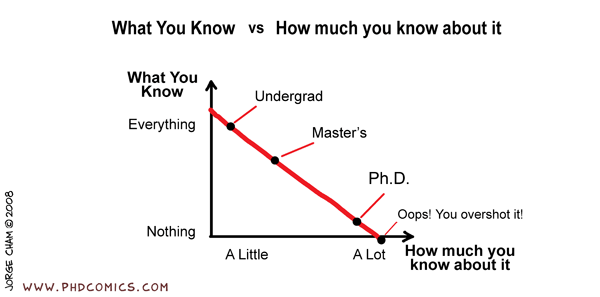
\includegraphics[width=0.7\linewidth]{Figures/comic.png}
\end{figure}

A common joke made about completing a PhD is that it teaches you a great deal about an insignificantly tiny slice of a field.
I would like to think I've come out a bit better than that (I know slightly less than a great deal about at least two tiny slices of chemistry), which I attribute almost entirely to my supervisor, Jonathan White.
I was lucky enough to stumble (literally, after a 21\textsuperscript{st} birthday the night before) into his group as a na\"ive Masters student, where I was immediately struck by the diversity of projects and people in the group.
From radiochemistry to photovoltaics, it seemed Jonathan could do anything.
I tried to imbibe as much of this attitude as I could during my Masters and PhD, sometimes ending up with a bit too much on my plate.
Nonetheless, thanks to Jonathan's wise counsel, I was able to tie almost all of the loose ends and disparate projects into this thesis.
I think this hunger for knowledge and eye for serendipity is one of the greatest gifts a supervisor could bestow on a PhD student, and for this I thank him profusely.

I also thank my PhD committee members, Brendan Abrahams and Uta Wille.
I genuinely looked forward to and enjoyed our annual progress meetings.
You both always provided such wonderful ideas and tangents for my projects, which I would never have otherwise thought of pursuing.
Along with Jonathan, you both helped to expose me to your respective areas of expertise, and I look forward to taking some of that knowledge with me to my first post-doc role.
Of course I shouldn't need to mention the incredible support and kindness you showed me.
I suppose I'm lucky I never had to, but I wouldn't have hesitated to come to either of your with any issues.
So thank you both, I couldn't have done it without you.

I owe a great deal to Colin Skene, for all the hands-on training throughout my Masters.
He also taught me the value of scientific rigour and detailed record-keeping, which I've tried to maintain as best as I can.

To all the members of the White group, past and present, thank you.
It's been an honour to work alongside such accomplished scientists, and your friendship is truly appreciated.
A special mention for the honorary White Walkers, Michael Ricca and Tze Cin Owyong, who have been a perpetual source of good times.
I will greatly miss our nights at Naughton's.

I thank all the wonderful friends I've made in the School of Chemistry.
Pre-COVID Friday Frothies were a monthly highlight, and the kick-ons to whichever watering hole happened to be open always reassured me that I had fallen into an excellent cohort.
On that note, I should also thank all the bar staff at Naughton's, The Clyde, Bobbie Peel's, and The Castle for so tactfully dealing with us rowdy chemists, and our heated late-night discussions over DFT functionals.

Thank you to my family, for 27 years of love and support, and for instilling in me the value of education.

Finally, I thank my loving partner, Alex Cummaudo.
You've taught me so much throughout our time together, not just about \LaTeX{}, but about persistence, compromise, and the value of family.
I'm so proud that I got to complete my PhD side by side with you, and I look forward to many more years with you and Pickles 
\includegraphics[width=1em]{Figures/pickles.png}.
}
\clearpage  % End of the Acknowledgements
%% ----------------------------------------------------------------

\pagestyle{fancy}  %The page style headers have been "empty" all this time, now use the "fancy" headers as defined before to bring them back


%% ----------------------------------------------------------------
%\lhead{\emph{Contents}}  % Set the left side page header to "Contents"
\tableofcontents  % Write out the Table of Contents

%% ----------------------------------------------------------------
%\lhead{\emph{List of Figures}}  % Set the left side page header to "List if Figures"
\listoffigures  % Write out the List of Figures

%% ----------------------------------------------------------------
%\lhead{\emph{List of Tables}}  % Set the left side page header to "List of Tables"
\listoftables  % Write out the List of Tables

%% ----------------------------------------------------------------
\setstretch{1.5}  % Set the line spacing to 1.5, this makes the following tables easier to read
\clearpage  % Start a new page
%\lhead{\emph{Abbreviations}}  % Set the left side page header to "Abbreviations"
\listofsymbols{ll}  % Include a list of Abbreviations (a table of two columns)
{
% \textbf{Acronym} & \textbf{W}hat (it) \textbf{S}tands \textbf{F}or \\
\textbf{LAH} & \textbf{L}ist \textbf{A}bbreviations \textbf{H}ere \\

}

%% ----------------------------------------------------------------
\clearpage  % Start a new page
%\lhead{\emph{Constants}}  % Set the left side page header to "Physical Constants"
\listofconstants{lrcl}  % Include a list of Physical Constants (a four column table)
{
% Constant Name & Symbol & = & Constant Value (with units) \\
Speed of Light & $c$ & $=$ & $2.997\ 924\ 58\times10^{8}\ \mbox{ms}^{-\mbox{s}}$ (exact)\\

}

%% ----------------------------------------------------------------
\clearpage  %Start a new page
%\lhead{\emph{Symbols}}  % Set the left side page header to "Symbols"
\listofnomenclature{lll}  % Include a list of Symbols (a three column table)
{
% symbol & name & unit \\
$a$ & distance & m \\
$P$ & power & W (Js$^{-1}$) \\
& & \\ % Gap to separate the Roman symbols from the Greek
$\omega$ & angular frequency & rads$^{-1}$ \\
}
%% ----------------------------------------------------------------
% End of the pre-able, contents and lists of things


%% ----------------------------------------------------------------
\mainmatter	  % Begin normal, numeric (1,2,3...) page numbering
\pagestyle{fancy}  % Return the page headers back to the "fancy" style

% Include the chapters of the thesis, as separate files
% Just uncomment the lines as you write the chapters

%\part{Background}
\begin{refsection}

\chapter{Introduction}

The importance of non-bonding interactions in our world simply cannot be overstated.
While we may think of the more familiar covalent and ionic bonds as the core of chemistry, more often than not it is non-bonding interactions that dictate the nature of substances, from bulk properties such as tensile strength, to microscopic phenomena like protein-ligand interactions.

At a fundamental level, all non-bonding interactions (indeed, conventional bonding too) are attributable to the electrostatic force.
However, it is more convenient to broadly categorise interactions based on strength and structural motifs that are common to each class.
Such classes include dispersion forces, dipole-dipole interactions, and H-bonding.
In the 19th century, it became apparent that these classes paint an incomplete picture of intermolecular bonding.
As part of their investigation into solvent effects on the colour of iodine solutions in 1949, Bensei and Hildebrand invoked the concept of ``charge-transfer'' complexes to explain the association of molecular iodine with nucleophililc solvent molecules.\autocite{Benesi1949}
Although the electrophilic nature of molecular halogens was already well appreciated with respect to reactivity, this appears to be the first acknowledgement that this understanding could be applied to ground state complexes.
In support of this, Hassel and Hvoslef elucidated the structure of a 1:1 complex of molecular bromine and 1,4-dioxane in 1954, and observed an unusally strong interaction between the two molecules.\autocite{Hassel1954}
The crystal was comprised of long chains of monomers (\cref{fig:hassel-xray}), exhibiting a very short O\dots Br contact (2.71\AA, the sum of the VDW radii is 3.37\AA), and a slightly lengthened Br--Br bond (2.31\AA~vs 2.28\AA~in gaseous bromine).

\begin{figure}[ht]
  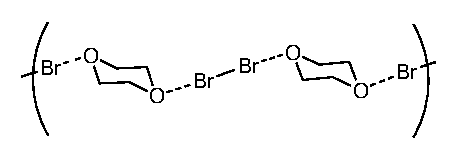
\includegraphics[width=0.6\columnwidth]{Figures/hassel-xray.eps}
  \caption{Long chains of molecular bromine and 1,4-dioxane, observed by Hassel and Hvoslef.}
  \label{fig:hassel-xray}
\end{figure}

In the subsequent years, a wide variety of names and labels were applied to the ``charge-transfer'' phenomenon, including ``lock and key'', ``donor-acceptor'', and ``filling of antibonding orbitals'', as summarised in Bent's excellent 1968 review\autocite{Bent1968}.
The term ``halogen bonding'' (X-bonding) only gained widespread acceptance in 1983 after the publication of the review of Dumas, Gomel, and Guerin.\autocite{Dumas1983}
The term deliberately evokes similarity to the better known concept of hydrogen bonding, as the two phenomena are of comparable strength and, importantly, directionality.
In 1998 Anthony C. Legon again used the term to describe the attractive interaction between halogens and Lewis bases in prereactive complexes, harking back to the original understanding of electrophilic halogens as a primarily reactive phenomenon.\autocite{Legon1998,Legon1999}
In the following years, the potential of X-bonding was more fully recognised, with applications in supramolecular chemistry and self-assembly\autocite{Corradi2000,Metrangolo2008,Priimagi2013}, catalysis and bond activation\autocite{Walter2011,Soloshonok2017,Takagi2017}, and molecular sensing and recognition\autocite{Cornes2017,VargasJentzsch2013,Borissov2017}.

From X-bonding grew the related concepts of chalcogen (Ch-), pnicogen (Pn-), and tetrel bonding (T-bonding), as the electrophilic nature of these elements was discovered.\autocite{Murray2007}
Similar applications have also been found for these classes of noncovalent interactions, Ch-bonding in particular.\autocite{Fanfrlik2014,Garrett2016,Ho2016,Wonner2017,Mitchell2017,Benz2017,Biot2018,Ho2017}

\section{Chalcogen Bonding}
Ch-bonding is the attractive interaction between a Lewis base and a chalcogen atom bearing an electron withdrawing substituent.
The terminology of Ch-bonding partners is perhaps counterintuitive, as donors and acceptors are named by analogy with H-bonded equivalents.
Note this is contrary to the formal flow of electron density; Ch-bond \emph{donors} bear vacant \emph{acceptor} orbitals, while Ch-bond \emph{acceptors} are \emph{donors} of electron density.
For the purposes of this report, ``donor'' will refer to the Lewis acidic chalcogen species.

\subsection{Mechanisms}
As was discussed in the introduction, all intermolecular (and indeed \emph{intra}molecular) forces are manifestations of the electromagnetic force.
Nonetheless, it is more convenient to categorise energetic contributions to any given interaction as orbital, electrostatic, or dispersion mediated, as there are marked differences in strength and directionality between them.
Historically, X- and Ch-bond interactions were understood to be primarily due to orbital overlap and resulting charge transfer.
Evidence for this included the lengthening of the X--X bond corresponding to increased occupation of the $\sigma^{\star}$(X-X) orbital due to the incoming lone pair (this was observed in Hassel and Hvoslef's original work\autocite{Hassel1954}).
Characteristic charge transfer bands are also observed in the UV-vis spectra of halogen solutions.\autocite{Blackstock1987}

Such evidence of orbital contributions is not, however, common to all systems displaying X- or Ch-bond interactions.
The iodoperfluoroalkanes and arenes studied by Resnati et al show no charge transfer bands in UV-vis spectra, yet are exceptionally strong X-bond donors.\autocite{Yan2014}
Jane Murray and Peter Politzer have advocated for an alternative, primarily electrostatic explanation of X- and Ch-bond interactions.\autocite{Murray2008,Murray2009}
They propose that a positively charged $\sigma$-hole is generated along the extension of a $\sigma$ bond to an electron withdrawing substituent, due to polarisation of the bonding orbital.
This also adequately explains the strength and directionality of these interactions.

An interpretation which has not attracted as much attention is that of dispersion forces.

While the varying contributions from each of these factors can be dissected computationally via pertubation methods, experimental evidence is surprisingly sparse.
Pascoe, Ling and Cockroft, however, devised an elegant experiment to quantitatively determine energetic contributions.\autocite{Pascoe2017}
\textsuperscript{19}F NMR was used to determine the relative populations of two conformors of a "molecular balance", one bearing a Ch-bond interaction, one not.
Interaction energies were thus derived, and found to be more or less invariant with respect to the solvent.
This appeared to rule out electrostatic contributions, as solvent dipole moment and bulk polarisability would otherwise have a large effect on the position of the equilibrium.
These results also suggest that dispersion plays only a minor role, for similar reasons.

DFT was used to further probe the dispersion contribution.
Free energies were calculated using functionals which both did, and did not include dispersion corrections, and the values compared to the experimental results.
The non-dispersion corrected B3LYP functional gave superior correlation with experiment than did either M06-2X and $\omega$B97-D, both of which include dispersion.
This provided additional evidence that, in the systems studied, the major contributor to the interaction is orbital overlap and charge transfer.

Although current evidence points towards these interactions being primarily orbital related, the electrostatic ``$\sigma$-hole'' terminology of Politzer and Murray has stuck, and the term is now used to encompass the whole gamut of X- Ch- Pn- and T-bonding interactions.

\section{Applications of Ch-Bonding}
Ch-bonding, and by extension, all $\sigma$-hole interactions can theoretically be applied to any formal Lewis acid-base system.
They are especially attractive as a hydro\emph{phobic} complement to H-bonding interactions, which are generally considered to be hydro\emph{philic}.
The following are brief summaries of existing applications in the literature.

\subsection{Materials}
The major applications of $\sigma$-hole interactions have so far been in the realm of crystal engineering.
Early work by \citeauthor{Corradi2000} showed that halogen bonding was able to outcompete H-bonding in the formation of supramolecular architectures.\autocite{Corradi2000}
A review by \citeauthor{Metrangolo2008} summarised the forms that are accessible using X-bonding to direct crystal growth.\autocite{Metrangolo2008}
1D, 2D, and 3D architectures are able to be generated using appropriate X-bond donors, and these show potential in the design of liquid crystals, organic semiconductors and paramagnetic materials.
A more recent review by the same group described applications in anion transport, and luminescent and photoresponsive crystals.\autocite{Priimagi2013}
The group of Stefan Matile has further explored anion transport, and has published a review comparing X-bonding with other hydrophobic interactions such as anion-$\pi$ and anion-macrodipole interactions.\autocite{VargasJentzsch2013}

Ch-bonding, too, has been investigated with respect to materials chemistry.
\citeauthor{Fanfrlik2014} demonstrated the importance of Ch-bonding on the crystal packing of thiaboranes.\autocite{Fanfrlik2014}
They found that the sulfur-based $\sigma$-hole was sufficiently strong to interact with the weakly basic $\pi$ electrons of a phenyl group, with contacts as short as 3.2\AA~being observed.

In 2016, \citeauthor{Ho2016} published their work into tellurium-based Ch-bonding.\autocite{Ho2016}
Their scaffolds are based on an iso-tellurazole N-oxide, which reversibly forms macrocyclic structures that persist in both gas and solution phase.
The macrocycles were found to coordinate \ce{Pd2+}.
This is particularly interesting, as the tellurium atoms are simultaneously behaving as a Lewis acid and base.
The authors point out that such soft macrocycles are quite rare, and their work could facilitate further studies of transition metals in a soft coordination environment.
They went on to investigate benzo-fused derivatives of iso-tellurazoles, as well as selenium analogues, which crystallised to form macromolecular pores and voids.\autocite{Ho2017}

The Taylor group has been active in the development of X- and Ch-bonding molecular sensors.
Early work demonstrated that X-bonding tridentate ligands (reminiscent of enterobactin) showed moderate selectivity for \ce{Cl-}.\autocite{Dimitrijevic2010}
They later developed bidentate Ch-bonding ligands which exhibited a tenfold increase in association constant with respect to chloride.\autocite{Garrett2015a,Garrett2016}

Similar results have been achieved by the Beer group, who have developed X-bonding sensors for the perrhenate anion.\autocite{Cornes2017}
These sensors are based on functionalised cyclodextrins, and are even more sensitive than the corresponding H-bonding analogues.
The group has also use iodotriazole scaffolds to chelate anions.\autocite{Borissov2017}
Incorporation of a chial binapthol moiety was shown to differentiate between enantiomers of chiral anions.

The role of selenium-based Ch-bonding on the crystal structure and mechanism of the drug ebselen was demonstrated by Thomas et al.\autocite{Thomas2015}
Interestingly, the Lewis acidity of the $\sigma$-hole was invoked as an explanation of the antioxidant properties of the drug.

\subsection{Catalysis and bond activation}
In 2008, halogen bonding was first applied to a Hantzsch ester reduction of a quinoline derivative.\autocite{Bruckmann2008}
This reaction is well characterised and understood, and has been catalyzed with a variety of Br\o nsted and Lewis acids.
The X-bond donors chosen were perfluoroiodoalkanes, and high conversions were achieved with modest catalyst loadings of 10\%.

In 2011, a modified Ritter reaction was devised wherein benzhydryl bromide was activated by a dicationic imidazolium-based X-bond donor to give the carbocation intermediate, which was then captured by acetonitrile and then hydrolysed to afford the amide product.\autocite{Walter2011}
This pioneering work was limited by the necessity of stoichiometric amounts of the X-bond donor, as it is consumed in the course of the reaction.

A similar alkylation of 1-chloroisochroman was achieved by the same group using a neutral perfluoroiodoarene X-bond donor in catalytic quantities.\autocite{Kniep2013}
The proposed mechanism is similar to the thiourea-catalysed reaction of \citeauthor{Reisman2008}\autocite{Reisman2008}, which has shown promise in asymmetric induction.
The authors noted issues with solubility of the perfluoroiodoarene catalysts, which is expected of such highly fluorinated compounds.

These reactions have all been repeated with Ch-bond donors in place of X-bonds.

The quinoline reduction was sucessfully catalysed by a dithiophene system by \citeauthor{Benz2017}. in 2017\autocite{Benz2017}, and then again by the same group with a benzodiselenazole.\autocite{Benz2017a}
With the increased selectivity and strength of the Se-based Ch-bonding catalyst compared to the X-bonding perfluoroiodoalkane, the authors were able to reduce the catalyst loading to 1\%.

\citeauthor{Wonner2017} developed a selenated bisbenzimidazolium Ch-bonding catalyst for the alkylation of 1-chloroisochroman, and solvolysis of benzyhydryl bromide.\autocite{Wonner2017,Wonner2017a}
Although the best results were observed with the dicationic catalysts, conversion was also achieved with a neutral bisbenzimidazole catalyst, providing further evidence that the catalytic Lewis-acid site is indeed the $\sigma$-hole.
For a given row in the periodic table (i.e. comparing a Se-based donor to a Br-based donor), Ch-bonding appeared to give superior results to X-bonding, as measured by \% yield.

An unusal manifestation of X-bonding is in the self-disproportionation of enantiomers, as reported by \citeauthor{Soloshonok2017}.\autocite{Soloshonok2017}
They observed spontaneous enrichment of one enantiomer of mebroqualone upon chromatography using an achiral solid phase, which they attributed to the formation of diasteromeric X-bonded oligomers.
This phenomenon has been observed in compounds capable of interacting through H-bonding or strong dipole-dipole interactions.

\subsection{Biological systems}

\subsubsection{Proteins}
While we usually think of the tertiary structure of proteins as being dominated by H-bonding and hydrophobic effects, there is increasing evidence that Ch-bonding plays an important role as well.
This is not unexpected, as sulfur, a component of both cysteine and methionine, is known to form Ch-bonds in small molecules.
In the early days of Ch-bonding interactions (2001, before the name had come into common use) \citeauthor{Iwaoka2001} published an analysis of 604 protein structures in the Protein Data Bank (PDB).\autocite{Iwaoka2001}

A remarkable number of close contacts (sum of Van der Waals radii plus 0.5\AA) between sulfur and Lewis basic (X) atoms were identified in the structures, with 33\% of cysteine residues and 22\% of methionine residues showing a close contact.
Furthermore, the geometric parameters of these contacts were studied, with more than half of all contacts having a S--S--X (X=O,N) of 150--180\degree.
The observed contacts were ascribed to a $\pi$(C=O)$\rightarrow \sigma^{\star}$(S--S) interaction, in contrast to the $n(X) \rightarrow \sigma^{\star}$(S-X) interaction which dominates in small molecules.
Also contrary to the case of small molecules, the authors suggest that the orbital component of the interaction is small, though important for establishing the directionality of the interaction.
Dispersion appears to be the major stabilising force, as optimization using a non-dispersion corrected level of theory gave unrealistically large distances.

The differences between Ch-bonding in proteins and small molecules is likely due to variation in orbital energies in the functional groups which are found in each class.
While small molecule Ch-bond donors are characterised by easily accessible, low energy $\sigma^{\star}$(Ch--X) orbitals, these are simply not found in proteins.
Instead, donors are characterised by $\sigma^{\star}$(S--S) or $\sigma^{\star}$(S--C) orbitals, which are much higher in energy and less accessible to acceptors.
Ch-bond acceptors, too, are markedly different between small molecules and proteins.
In general, the HOMO of a system (the most Lewis basic site) is dominated by lone pairs.
This is observed in most small molecules, as they form Ch-bonds through these lone pairs.
However, the amide bond, which is ubiquitous in proteins, shows an unusual inversion in orbital energies.
The $\pi$(C=O) orbital is elevated with respect to the lone pair according to MP2 calculations, making it the more basic site.
Structural data supports this assertion, as the Ch-bond donor usually approaches the top of the C=O bond in proteins, rather than the usual approach towards the oxygen lone pair.\autocite{Iwaoka2012}

It is worth noting that selenium is also found in proteins as selenocysteine and selenomethionine.
This would be expected to be an even stronger Ch-bond donor.
However, selenoproteins are relatively few in number, precluding such extensive statistical analysis.\autocite{Iwaoka2015}
They are only mentioned here for the sake of completeness.

\emph{Intra}molecular interactions are just one instance of Ch-bonding in biological systems.
Proteins often interact with ligands or substrates through H-bonds, so it is reasonable to propose that Ch-bonding could be applied in this field as well.
Indeed, a protein-ligand Ch- and X-bonding interaction was used to target the gatekeeper methionine (MET146) residue of c-Jun N-terminal kinase 3 (JNK3) in a model study by \citeauthor{Lange2015}.\autocite{Lange2015}
In this work, a protein$\rightarrow$ligand Ch-bond was used to stabilise the interaction.
Inhibition of a cysteine protease using a variety of sulfur-containing heterocyclic ligands was also investigated.\autocite{Giroud2017}
These ligands formed ligand$\rightarrow$protein Ch-bonds, complementary to the the work by Lange.
Non-conventional protein-ligand interactions are summarised in a comprehensive review by Beno et al.\autocite{Beno2015}

\subsubsection{Nucleic acids}
Nucleic acids represent another application of Ch-bonding in biology.
In addition to their crucial role in the storage of genetic information, they have also been investigated as a structural material in nanotechnology.
The ubiquity of H-bonds in nucleic acid complexes suggests that $\sigma$-hole interactions may also be used to direct formation of these complexes.
X-bonding was indeed able to be used to direct formation of a Holliday junction between two DNA strands.\autocite{Voth2007}
Holliday junctions are branched nucleic acid structures that appear in many biological processes includin recombination and double-strand break repair.
They are also useful as building blocks for DNA nanotechnology, where their self assembly and predictable gemoetry are exploited.
The authors estimated that the X-bonding interaction (mediated through a bromo-substituent) was 2--5 kcal/mol stronger than the corresponding H-bond.
A 2017 review identified a further 21 X-bonded nucleic acid structures.\autocite{Kolar2017}

LOTS TO TALK ABOUT. SEE \cite{Sharma2020} AND RELATED REFERENCES \cite{Farrell2018,Mai2019,Peng2020,Fang2019,Uleany2020,Sun2012,Hassan2010,Vazquez-Mayagoitia2009,Salon2007,DeBoer2007,Sun2019,Faustino2014,Lee2015,Conlon2019,Parker2012}

\section{Experimental methods}
As mentioned above, X- and Ch-bonded interactions were originally identified crystallographically, with additional spectroscopic evidence being present.
These pioneering methods have not changed a great deal, and x-ray crystallography is still the most powerful tool we have to study these interactions.
We also use a number of spectroscopic techniques to probe the nature of Ch-bonding.
Some of the methods used in this work go beyond the typical level encountered in postgraduate study, so a brief explanation of each is included here.

\subsection{X-ray crystallography}
Single crystal x-ray crystallography is the main experimental technique used in this work.
It allows unambiguous determination of the structure of compounds (including stereochemistry), and potentially extremely accurate measurement of geometric parameters such as bond lengths.
Practically speaking, a structure is determined by mounting a single crystal of a compound on a goniometer which can rotate the crystal through any orientation, then observing the position and intensity of diffracted x-ray beams.
Rotating the crystal allows different diffraction spots to be observed, and a more complete dataset to be collected.
The position of the diffraction spots provides information about the size and shape of the unit cell, and the intensities provide information about the internal structure i.e. the locations of the atoms in the unit cell.
A full discussion of the mathematics of diffraction is outside the scope of this thesis, but the interested reader is referred to \citetitle{Stout1989} by \citeauthor{Stout1989}.\autocite{Stout1989}

\subsubsection{Charge density refinement}
Fundamental to the technique of x-ray structure determination is the process of refinement, by which parameters of the model (typically the molecular geometry) are optimised to reproduce the observed intensity data as well as possible.
Mathematically, this is performed as a least-squares optimisation, where the function
\begin{equation}
    \sum^{m}_{r=1} w_{r} \left(f_{\mathrm{obs}, r} - f_{\mathrm{calc}, r} \right) ^{2}
\end{equation}
is minimised, where $f_{\mathrm{obs}, r}$ corresponds to the observed intensity, and $f_{\mathrm{calc}, r}$ corresponds to the intensity calculated from the model by Fourier transform.
$w_{r}$ is a weighting function used to reflect the confidence in any given observed data point.

Assuming the measured intensities are free of any error,\footnote{This is practically never the case, but careful measurement and modern corrections can approach this limit.} this function could theoretically be minimised to zero i.e. the model is a complete and true representation of the crystal.
The question then becomes, how do we determine $f_{\mathrm{calc}, r}$ from our model?
To answer this, we must consider what our model actually \emph{is}.

The simplest refinement model consists of atomic coordinates for each atom, plus an overall scale factor (for now we will neglect the anisotropic displacement parameters and chemical occupancies).
However, in order to calculate $f_{\mathrm{calc}, r}$ by Fourier transform, we must introduce some description of what the atoms which we are locating ``look like''.
This forms a hidden, but still crucially important, part of the model.
Typically, atoms are described in reciprocal space as spherically symmetric functions whose contribution to $f_{\mathrm{calc}, r}$ is only dependent on $(\sin\theta)/\lambda$ (\cref{fig:scatterf}).
This is a consequence of the fact that x-rays are scattered by the \emph{electron cloud} of the atom.\footnote{X-rays have much less energy than the mass-energy of subatomic particles, so are scattered in the low energy limit of Compton scattering, known as Thompson scattering.
The scattering power of a particle is inversely proportional to the square of its mass, so the massive nuclei contribute negligibly to scattering compared to electrons.}
At $(\sin\theta)/\lambda = 0$ the scattering factor is equal to the number of electrons in the atom.
However, the finite size of the electron cloud causes destructive interference and attenuation of the scattering factor as $(\sin\theta)/\lambda$ increases, as x-rays scattered from one side of the electron cloud will be out of phase with those scattered from the other side.
Contrast this with neutron diffraction, where the neutrons are scattered predominantly by the point-like nucleus, affording a flat scattering function in reciprocal space.
There is almost no destructive interference, and thus neutron crystallography is characterised by an abundance of strong high angle data.
The scattering factor functions for all elements of the periodic table (and many ions) have been calculated based on theoretical electron densities from Hartree-Fock wavefunctions, and the results are available in the International Tables.\autocite{IntTabCIntensityofdiffractedintensities}
These functions are mercifully incorporated in crystallographic refinement software, shielding them from the user.

\begin{figure}
    \centering
    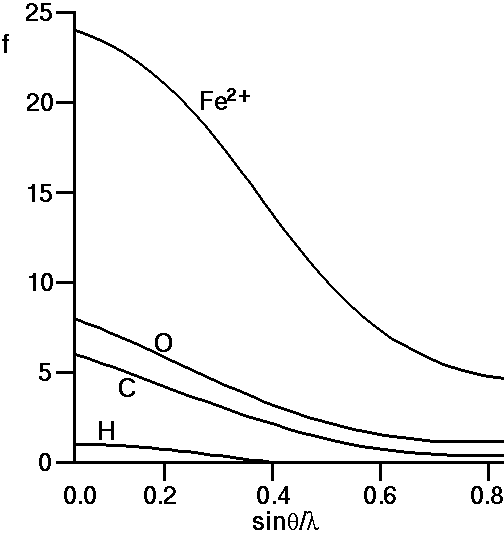
\includegraphics[width=0.5\linewidth]{Figures/scatterf.png}
    \caption{Scattering factors for some atoms as a function of $(\sin\theta)/\lambda$.}
    \label{fig:scatterf}
\end{figure}

From the above discussion, one major shortcoming of this approach should be clear.
Namely, that the electron density of bonded atoms is \emph{not} spherically symmetric.
Perturbations such as bonding electron density, lone pairs, and indeed $\sigma$-holes can, and do, affect the observed scattering factors of atoms, which are not taken into account in typical refinement software.
An extreme case of this, and one that is familiar to any crystallographer, is that of the hydrogen atom.
As the lightest element with only one electron, perturbations due to bonding have an enormous effect, such that the typical \ce{C-H} bond length is underestimated by some 0.13~\AA.\autocite{Cooper2010}
A subtler but more interesting manifestation of this was identified in 1968 by \citeauthor{Coppens1968EvidenceEffects}.\autocite{Coppens1968EvidenceEffects}
X-ray and neutron structures were determined for a crystal of 1,3,5-triazine, and inspection of the difference (a so-called $\mathrm{X}-\mathrm{N}$ map) revealed unusual systematic variations in the anisotropic displacement parameters.
The nitrogen atoms were deformed radially to the ring, while the carbon atoms were deformed tangentially (\cref{fig:x-n-coppens}).
This is chemically intuitive, as we would expect the lone pairs of the nitrogens to extend radially, while the $\pi$-electrons of the carbon atoms would form a ring.
The fact that these deformations were incorporated into the anisotropic displacement parameters in the x-ray structure highlights a deficiency of the typical method of refinement.

\begin{figure}
    \centering
    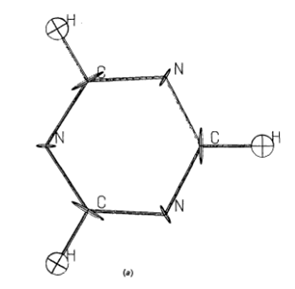
\includegraphics[width=0.5\linewidth]{Figures/x-n-coppens.png}
    \caption{$\mathrm{X}-\mathrm{N}$ map of 1,3,5-triazine, reproduced from \citeauthor{Coppens1968EvidenceEffects}.\autocite{Coppens1968EvidenceEffects}}
    \label{fig:x-n-coppens}
\end{figure}

Evidence for aspherical atoms can even be traced back to seminal studies performed by the great \citeauthor{Bragg1920}, in which the famous 222 reflection of a diamond crystal was observed.
The 222 reflection is a systematic extinction of the $Fd\bar{3}m$ space group to which diamond belongs, but its absence is based on the assumption of spherical atoms.
In diamond, the carbon atoms are actually tetrahedral in form due to the bonding electron density, which lowers the space group symmetry and causes the 222 reflection to be present, though very weak.\autocite{Bragg1920}
Though cutting edge for the time, Bragg's experiment was rather primitive, and multiple scattering likely contributed some intensity to the observed 222 reflection.
The observation was nonetheless correct, and the tetrahedral nature of the carbon atoms in diamond has subsequently been proven time and time again.

Although such perturbations generally only manifest in very high quality structures (aspherical atoms are typically the least of a crystallographer's worries), a number of methods have been proposed to improve refinements, and indeed gain further chemical knowledge from the experimentally determined aspheical electron density.
A simple approach is the use of tabulated aspherical scattering factors for atoms of distinct chemical types.
An example of this is the ELMAM2 database, developed by Jelsch and coworkers.\autocite{Domagaa2012}
The ELMAM2 database consists of experimentally derived scattering factors for all common atom types, with a focus on those found in amino acids and peptides.
A refinement using this database would begin by assigning a type to each atom, which can be done relatively easily using bonding geometries from a more primitive refinement.
This can afford substantial improvement in refinement statistics by providing a more accurate model, at a very modest computational cost.
The obvious drawback of this approach is that the scattering factors must already be tabulated, and the enormous diversity beyond the biochemically important C, H, N, and O precludes the assembly of a truly comprehensive database.
Furthermore, as the scattering factors are pre-tabulated, there is little chemical information that can be extracted from the model beyond somewhat improved precision in geometric parameters.

An improved approach is to compute scattering factors on a case-by-case basis.
This is the rationale behind Hirshfeld Atom Refinement (HARt), first developed by \citeauthor{Jayatilaka2008}.\autocite{Jayatilaka2008}
HARt is an iterative procedure in which the atomic coordinates from a spherical atom refinement (perhaps after correcting \ce{C-H} bond distances) are used to variationally calculate a wavefunction, from which is calculated an electron density and thus scattering factors.
These new scattering factors improve the model after refinement, from which is calculated a \emph{new} wavefunction, and so on until the cycles of least squares refinement and wavefunction calculations converge.
Clearly this repeated calculation of a wavefunction is computationally expensive, with even relatively simple molecules taking minutes.
Fortunately, however, even very inexpensive levels of theory tend to generate sensible densities for the ground state.
An advantage over the database approach is that one can capture unusual effects in the electron density (such as various non-bonding interaction), provided that they are correctly modelled by the underlying quantum chemistry theory used to generate the wavefunction.
However this raises a philosphical question: what exactly we are hoping to get out of this procedure?
It can certainly provide improved refinement statistics, including anisotropic refinement of hydrogens in agreement with neutron data, but if we are seeking chemical information about the system, we might as well simply use a gas-phase optimised wavefunction and dispense with the crystallography.

Related to this is the field of quantum crystallography, which differs somewhat in motivation, if not in methodology.
Quantum crystallography is concerned with extracting a wavefunction from diffraction data, rather than using a wavefunction to improve a crystallographic model.
Clearly there is significant overlap.
One method takes inspiration from perturbation theory, where, as in MP2, the Hartree-Fock wavefunction is taken as the zeroth order approximation.
The diffraction data is then used to construct a perturbative term, which introduces a degree of correlation to the wavefunction, bringing it closer to the truth (at least within the Born-Oppenheimer approximation).\autocite{Weiss1962}
Even with the power of modern computers, this is not an easy task, and quantum crystallography remains an active and exciting area of research.
It is also worth mentioning the x-ray constrained wavefunction method developed by \citeauthor{Grimwood2003}.\autocite{Grimwood2003}
This is simply a Hartree-Fock wavefunction calculations that is constrained \emph{via} a Lagrangian multiplier to reproduce the observed intensities in the experimental data, assuming there are no crystallographic artifacts in the data such as disorder or twinning.
That is to say, the crystal is simply comprised of infinitely repeating symmetry related molecular units.
The x-ray constrained wavefunction can be used to calculate a density, which can be used in a HARt-like procedure, which has been named x-ray wavefunction refinement (XWR).\autocite{Woinska2017}
Both quantum chemistry and crystallographic refinement codes have been implemented in the software package TONTO.\autocite{Jayatilaka2003}

Perhaps the most powerful approach for experimental crystallographers is that of multipole refinement using the formalism developed by Hansen and Coppens.\autocite{Hansen1978}
While superficially similar to quantum crystallographic approaches, no chemical restraint\footnote{This is not strictly true, as electroneutrality is routinely imposed as a constraint on multipole models.} is placed on the resulting electron density, allowing for the modelling of phenomena which are not described by \emph{ab inito} calculations.
The electron density is expanded in a series of atom-centered spherical harmonic basis functions, the local coordinate systems of which are often chosen to align with chemical features.
Each basis function requires two parameters for the occupancy and expansion, in addition to the position and anisotropic displacement parameters for each atom.
We therefore require a large number of observations to ensure the system is overdetermined, and can be treated in a least-squares manner.
Furthermore, the ADPs and dipolar basis terms are highly correlated, leading to an unstable solution if refined simultaneously (\cref{fig:adp-dipole}).
For this reason, it is critical to establish accurate atomic positions and ADPs before refining the multipole parameters and charge density.
Traditionally this was done using neutron data which, as mentioned above, is insensitive to electron density perturbations as neutrons are scattered almost exclusively by the nucleus.
Unfortunately neutron sources are notoriously expensive and low-flux, requiring extremely large crystals which introduces further errors due to extinction.
With the advent of modern x-ray diffractometer technology, we can luckily determine atomic coordinates and ADPs using x-ray data alone.
This is done using high angle reflections, which are dominated by core scattering and thus contain little data from the diffuse bonding electron density.
Core electron density is almost perfectly spherical, allowing ADPs to be correctly refined from this data.
With accurate atomic coordinates and ADPs in hand, hydrogen atoms can be located in the low angle data, and then the multipole parameters refined to convergence.
Multipole refinement can benefit enormously from an initial database model, particularly for hydrogen atoms, so it is no surprise that the techniques are often used sequentially.\autocite{Guillot2001,Volkov2006}
The resulting electron density can be used to characterise molecules and predict reactivity, particularly when interpreted within the powerful Quantum Theory of Atoms In Molecules frameork of Bader.\autocite{Bader1991}
The obvious attraction of this method is that it is almost entirely experimental.
However, the atom centered multipole functions and their resulting sum, while superficially resembling a wavefunction, is not antisymmetric and is therefore in violation of the Pauli exclusion priniciple.
It therefore cannot be used to determine \emph{all} properties of a system.

\begin{figure}
    \centering
    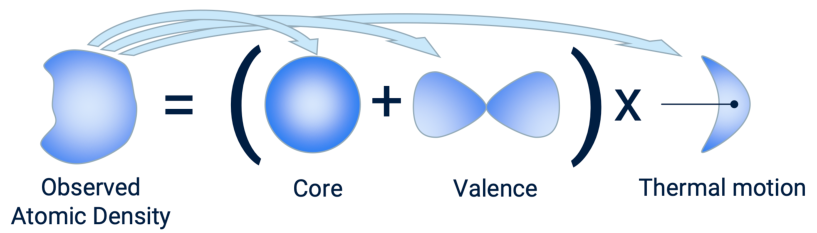
\includegraphics[width=0.6\linewidth]{Figures/valencevsthermaled.pdf}
    \caption{Thermal motion (described by anisotropic displacement parameters) and dipolar basis terms are highly correlated.}
    \label{fig:adp-dipole}
\end{figure}

\subsection{Nuclear Magnetic Resonance}
Nuclear magnetic resonance spectroscopy (NMR) is an essential tool for all organic chemists, as it is able to give relatively detailed structural information quickly and cheaply.
It is based on the magnetic moment of certain nuclei, which are usually randomly oriented but spontaneously align in the presence of a strong magnetic field.

\subsubsection{Solid State NMR}
The chemical shift of a nucleus is not a simple scalar quantity, as solution phase NMR experiments might suggest.
The shielding, and hence the effective magnetic field felt by the nucleus depends on the electronic environment around the nucleus, which is decidedly \emph{an}isotropic, therefore incapable of being expressed as a scalar.
Depending on the orientation of the electron cloud (and other shielding/deshielding influences) around the nucleus with respect to the magnetic field, different chemical shifts will be observed for the same nucleus.
This phenomenon is the chemical shift anisotropy of a nucleus, and it is described mathematically by a second rank tensor, which is geometrically depicted as an ellipsoid.

In a solution phase NMR experiment, rapid and random tumbling of the molecules averages out the anisotropy of each signal, affording a sharp peak at the isotropic chemical shift.
This can be simulated to some degree by magic angle spinning in solids experiments, but it is often the case that the chemical shift anisotropy is more interesting that the isotropic shift, so a solid phase NMR experiment is the only way to examine it.

The shape of the chemical shift tensor can provide insight into the electronic environment of a nucleus, with large shielding components often being aligned with electronic features such as bonds or lone pairs.
It is often convenient to define a principal axis system (PAS) for the tensor, consisting of two components which describe the longest and shortest axes of the ellipsoid, and the axis perpendicular to both.
The PAS of the chemical shielding tensor is denoted by the lowercase $x$, $y$ and $z$, and the components of the tensor which are aligned with these axes are labelled $\sigma_{xx}$, $\sigma_{yy}$ and $\sigma_{zz}$.
The laboratory reference frame is denoted by the uppercase $X$, $Y$ and $Z$, with the magnetic field $B_0$ being aligned with the $Z$ axis.
A common method for transforming one coordinate system to another is through the use of Euler angles $\alpha$, $\beta$ and $\gamma$, which define sequential right-handed rotations about the axes of the rotating frame.
As the chemical shielding is necessarily invariant to rotation about $Z$, we can dispense with the first of these angles $\alpha$, and simply refer to the latter two as the polar angles $\beta = \theta$ and $\gamma = \phi$.
The chemical shielding tensor is thus depicted in \cref{fig:chemical-shielding-tensor}, and this will be the convention used in this work.

\begin{figure}
  \centering
  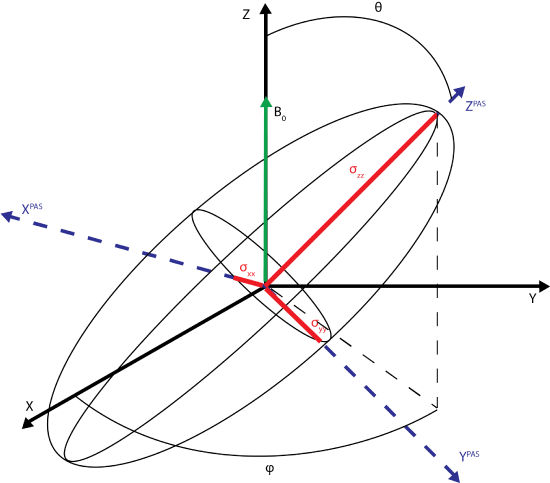
\includegraphics[width=0.4\linewidth]{Figures/Chemical_Shift_Tensor.png}
  \caption{Representation of the principal axis system (PAS, blue dotted lines) with respect to the laboratory reference frame (black solid lines). The polar angles $\theta$ and $\phi$ relate the former to the latter. The principal components of the tensor are shown in red, and the overall shape is shown by the black ellipses.}
  \label{fig:chemical-shielding-tensor}
\end{figure}

In almost all experiments, the chemical shielding tensor $\sigma$ is only indirected measured, \emph{via} the chemical shift $\delta$, which is defined with respect to a reference nucleus such that $\delta = \sigma_{\textrm{ref}} - \sigma_{\textrm{sample}}$.
As the coordinate system as described above is somewhat arbitrary, the IUPAC convention defines the three principal components of the chemical shift tensor $\delta_{11}$, $\delta_{22}$ and $\delta_{33}$ such that $\delta_{11} \geq \delta_{22} \geq \delta_{33}$.
The isotropic chemical shift is given by the average $\delta_{\textrm{iso}} = \frac{(\delta_{11} + \delta_{22} + \delta_{33})}{3}$.
There are two other conventions for describing chemical shift anisotropy, which are useful in different contexts.
The Herzfeld Berger convention represents the chemical shift in terms of the span of the signal $\Omega = \delta_{11} - \delta_{33}$ and the skew $\kappa = \frac{3(\delta_{22} - \delta_{\textrm{iso}})}{\Omega}$ where $\delta_{\textrm{iso}}$ is the same as in the IUPAC convention.
This is particularly useful for intuitively describing the powder lineshape formed by a given signal.
The other convention is the Haeberlen convention, which defines the three principal components as $|\delta_{zz} - \delta_{\textrm{iso}}| \geq |\delta_{xx} - \delta_{\textrm{iso}}| \geq |\delta_{yy} - \delta_{\textrm{iso}}|$, and the parameters $\delta = \delta_{zz} -\delta_{\textrm{iso}}$ and $\eta = \frac{\delta_{xx} - \delta_{yy}}{\delta_{zz} -\delta_{\textrm{iso}}}$.
This convention is most useful for describing the angular dependence of a chemical shift on the polar angles $\theta$ and $\phi$, which is given by the relationship\autocite{Haeberlen1976}
\begin{equation}
  \delta_{\textrm{obs}} = \delta_{\textrm{iso}} + \delta \left(\frac{3 \cos^2 \theta - 1 + \eta \sin^2 \theta \cos 2 \phi}{2} \right)
  \label{eqn:orientation-csa}
\end{equation}

In a non-spinning polycrystalline or amorphous powder, the above expression can be integrated over the range of chemical shifts to give the characterisitc powder lineshape see in \cref{fig:ssnmr-tensor}, reproduced from the work of Facelli, Grant, and Michl.\autocite{Facelli1987Carbon-13Determination}
The sample consists of randomly oriented tensors, all of which contribute to the signal.
The principal values of the tensor $\delta_{11}$, $\delta_{22}$ and $\delta_{33}$ correspond to the two extrema of the line, and the central peak.

\begin{figure}
  \centering
  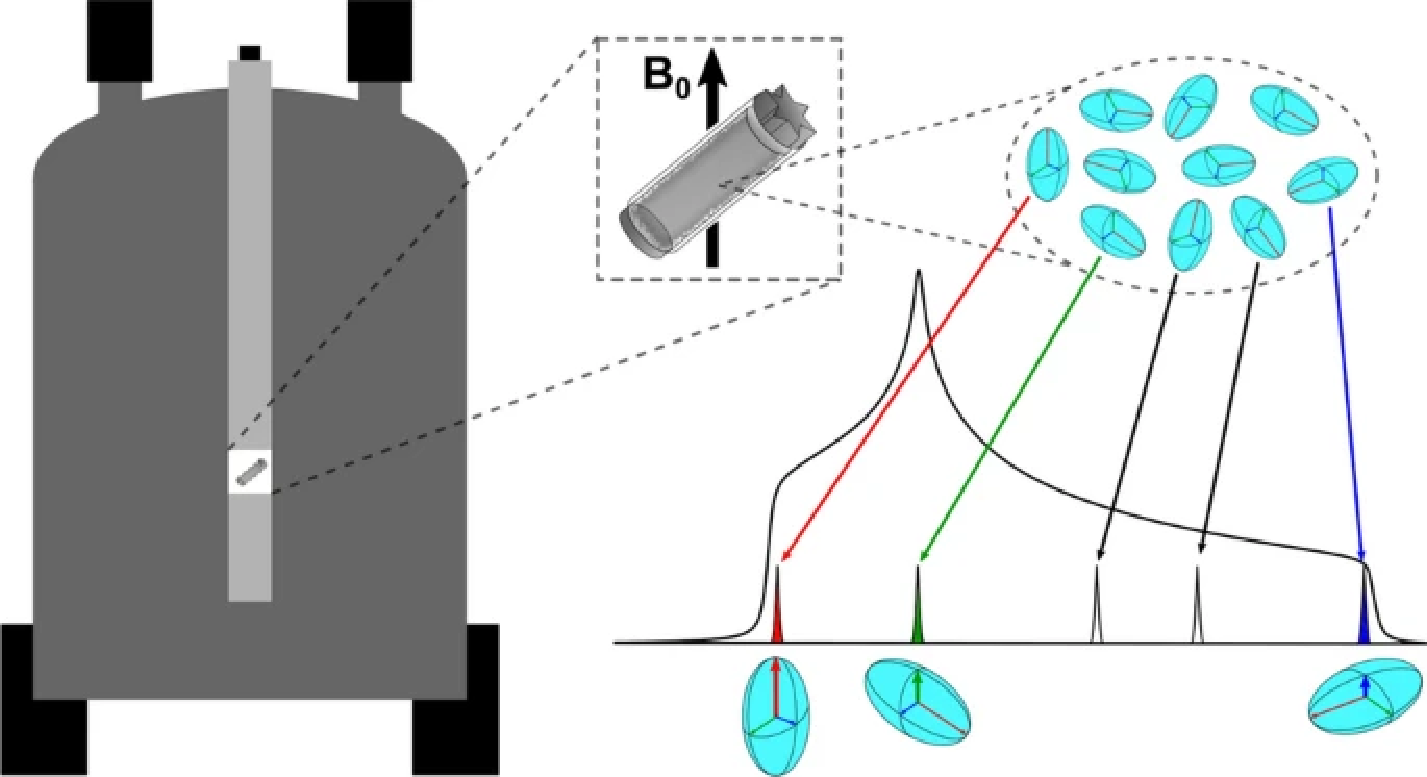
\includegraphics[width=0.45\linewidth]{Figures/ssnmr-tensor.pdf}
  \caption{Characteristic solid-state NMR powder lineshape for an asymmetric tensor e.g. in an alkene. The positions of the three principal values are shown.}
  \label{fig:ssnmr-tensor}
\end{figure}

The extremely poor S/N ratio (especially for a relatively insensitive nucleus like \ce{^{77}Se}) limits the utility of this method, as the radiated signal from the nuclei is spread out over a large bandwidth.
Spinning at the magic angle can improve the S/N ratio by partially averaging out the chemical shift anisotropy and dipolar relaxation.
Instead of the powder pattern, we instead observe a sharp isotropic chemical shift and a series of spinning sidebands which are separated from the isotropic peak by multiples of the spinning frequency.
The radiated power is thus concentrated in narrower bands, leading to a much improved S/N ratio.

An example is presented in \cref{fig:31P-ssnmr} of proton decoupled solid state \ce{^{31}P} spectra of barium diethyl phosphate, reproduced from the work of Herzfeld and Berger\autocite{Herzfeld1980SidebandAngle}.
In the first spectrum, no magic angle spinning was used, and the lineshape is characteristically broadened into an asymmetric peak (the powder lineshape).
Note the poor S/N ratio due to the broad peak.
The S/N ratio can be seen to improve as the spinning speed increases, and the sidebands become more sparse, affording a stronger signal overall.

\begin{figure}
    \centering
    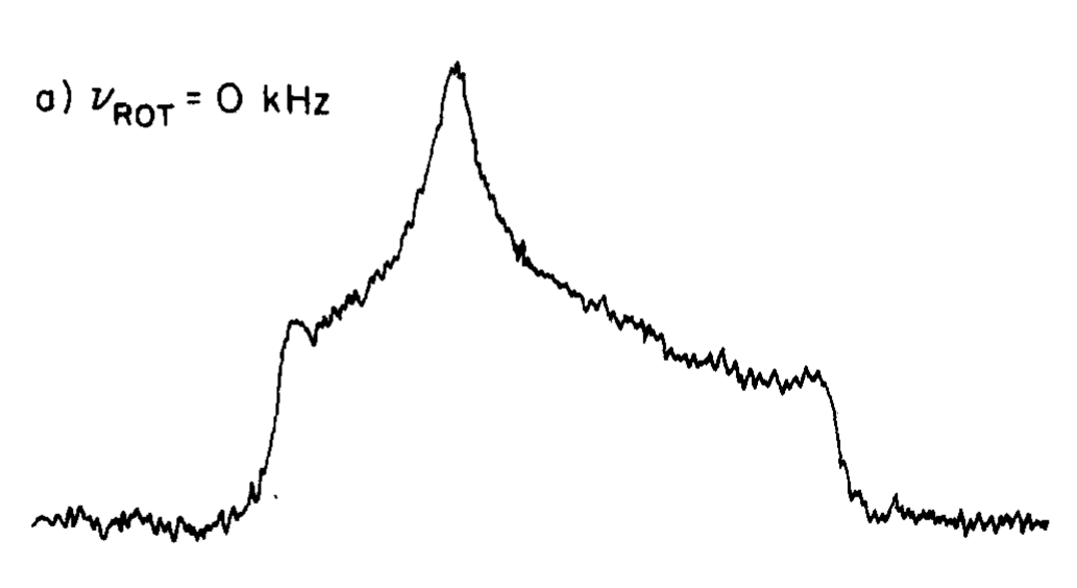
\includegraphics[width=0.45\linewidth]{Figures/31P-ssnmr-0khz.pdf}
    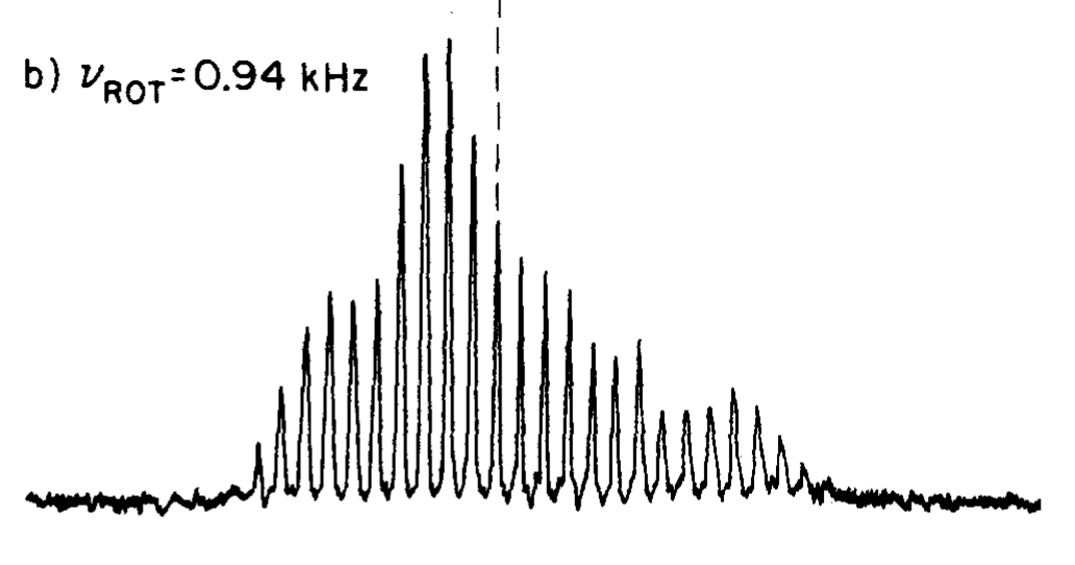
\includegraphics[width=0.45\linewidth]{Figures/31P-ssnmr-0.94khz.pdf}

    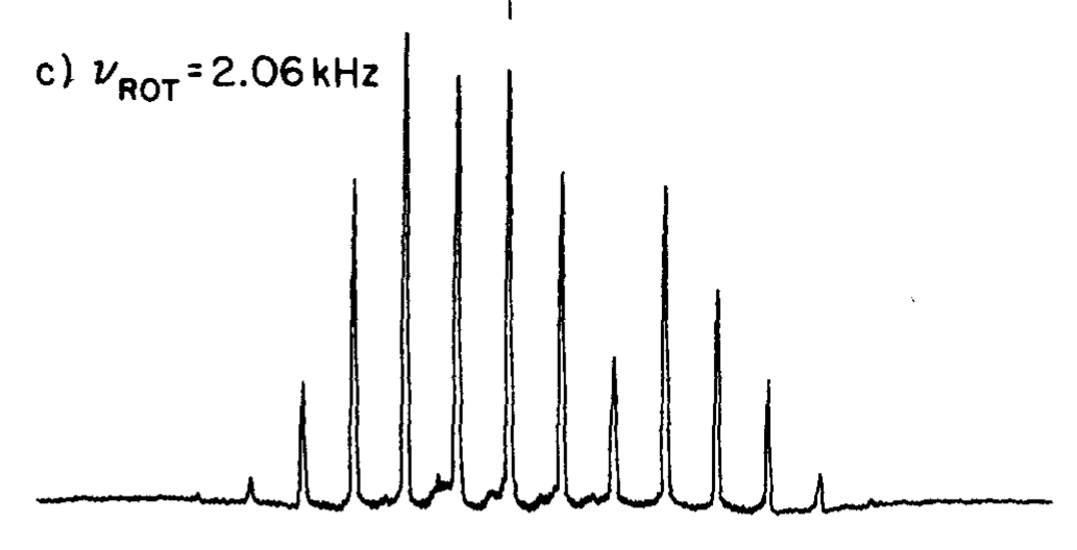
\includegraphics[width=0.45\linewidth]{Figures/31P-ssnmr-2.06khz.pdf}
    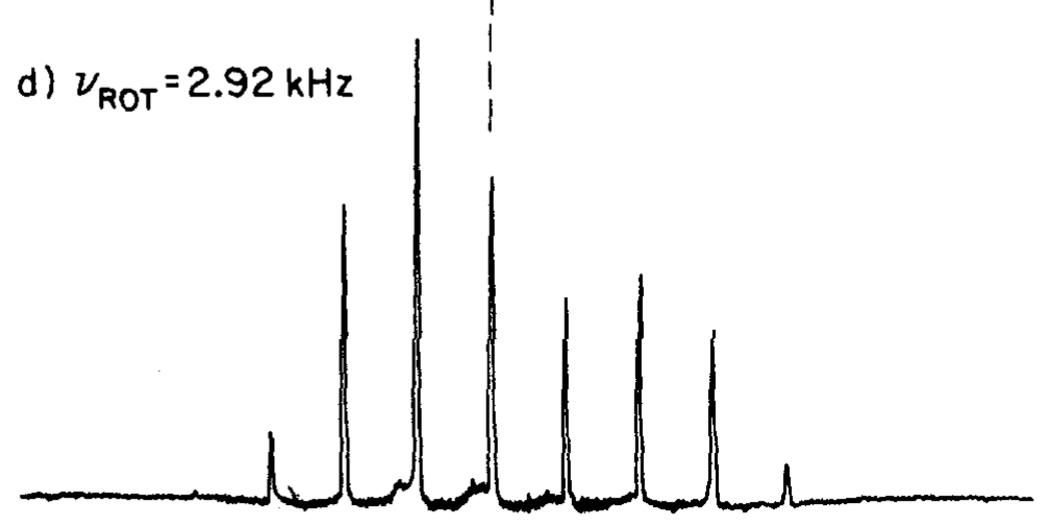
\includegraphics[width=0.45\linewidth]{Figures/31P-ssnmr-2.92khz.pdf}
    \caption{Proton decoupled solid state \ce{^{31}P} spectra of barium diethyl phosphate spinning at the magic angle, at the speed specified. The isotropic chemical shift is shown by the vertical dotted line.}
    \label{fig:31P-ssnmr}
\end{figure}

The principal values of the tensor are clearly easily obtained from a non-spinning sample, as they can practically be read off the spectrum.
However, the extremely poor S/N ratio (especially for a relatively insensitive nucleus like \ce{^{77}Se}) limits the utility of this method.
Spinning at the magic angle is clearly necessary to improve the S/N ratio, however this obscures the true locations of the extrema of the signal, therefore the values of $\delta_{11}$ and $\delta_{33}$, as well as modifying the position of the maximum ($\delta_{22}$).

There exist programs (such as SOLA, integrated within TopSpin by Bruker BioSpin) which can fit an experimental lineshape or sideband manifold affording the principal values of the tensor, however there is clearly a trade-off between obtaining a good S/N ratio and having enough sidebands within the limits of the signal for a meaningful fit.
Another issue is encountered with preferred orientation of crystallites, as in powder diffraction, which is not modelled in the fitting routine, leading to a poorer fit.
Perhaps the most fundamental issue stems from the fact that the sample is a powder of randomly oriented particles.
This means that the absolute orientation of the tensor with respect to the molecule cannot be determined from this kind of experiment.
Nonetheless, the \emph{shape} of the tensor is still valuable information that may be able to shed light on Ch-bonding in the solid phase.



\printbibliography[heading=subbibliography]
\end{refsection}

\begin{refsection}

\chapter[Simulating chalcogen bonding using molecular mechanics]{Simulating chalcogen bonding using molecular mechanics: A pseudoatom approach to model ebselen.}

This chapter was submitted to chemRxiv...

\section{Introduction}
Ebselen (\cmpd{ebs}) is a molecule that has piqued the interest of many medicinal chemists, in no small part due to its decidedly non-druglike appearance.
First synthesized in 1924, its unusual properties went more or less uninvestigated for more than 50 years.\autocite{Lesser1924}
Interest in ebselen boomed in the early 1980s, and since then it has been the subject of several studies into its synthesis, biological properties, and metabolism.\autocite{Weber1976,Renson1981,Muller1984,Wendel1984,Parnham1984,Engman1989,Schewe1995,Bhabak2010,Iwasaki2017}
Its biological activity can be broadly attributed to its ability to neutralize reactive oxygen species (ROS), reducing the level of oxidative stress to which cells are subjected.\autocite{Mugesh2000}
To this end, ebselen has been investigated for its neuroprotective, mood-stabilizing, anti-inflammatory, and anti-cancer properties.\autocite{Parnham1987,Kil2007,Singh2013,Azad2014,Parnham2000,Chantadul2020}
Recently it was identified as a compound of interest for the treatment of COVID-19, showing promising inhibition of the viral M\textsuperscript{pro} protease enzyme.\autocite{Jin2020}

The \emph{in vivo} antioxidant ability of ebselen is believed to be mediated through a catalytic cycle analogous to that of glutathione peroxidase (a selenoenzyme).\autocite{Antony2011}
The selenium-containing heterocycle is reductively opened to afford the free selenol, which is the active catalyst.
This is rapidly oxidised by ROS to a selenenic acid, which is then reduced back to the selenol by glutathione (GSH) via a selenenyl sulfide.
Its activity against a number of other targets appears to also be mediated through formation of a covalent complex via nucleophilic attack at the selenium.
There is also evidence that ebselen interacts with targets non-covalently.\autocite{Jin2020}
These interactions may include association with aromatic or hydrophobic residues, or H-bonding through the carbonyl.
Ebselen can also form non-covalent complexes with Lewis bases through an electrophilic $\sigma$-hole on the selenium atom, similarly to electron-deficient sulfur-containing molecules.\autocite{Thomas2015,Fellowes2019,Beno2015}

\begin{figure}
\centering
\replacecmpd{ebs}
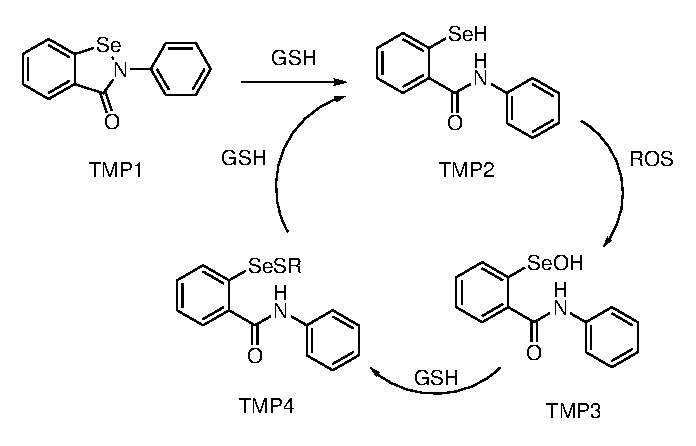
\includegraphics[scale=0.74]{Figures/ebs-cat-cycle.eps}
\caption{Catalytic cycle of ebselen \refcmpd{ebs} \emph{in vivo}.}
\label{fig:catcycle}
\end{figure}

Molecular modelling is a vital tool in drug development, allowing for rapid and broad-reaching screening of drug candidates against likely substrates at minimal cost and risk.
\emph{Ab initio} quantum methods (QM) are widely used to model small molecules (generally smaller than a few hundred atoms), where their accuracy and ability to describe quantum effects underlying photochemical properties and bond breaking/formation processes are critical.
They are however, computationally costly.
Molecular mechanics (MM), where systems are treated strictly classically, is a viable alternative for large systems.
The drawbacks are that MM relies on having an extensive parameter set (a ``force field'') to describe the system (which is not necessarily available, or applicable to the system at hand), and that descriptions of quantum effects often fail spectacularly.

Both of these issues are encountered when attempting to model ebselen using MM.
Firstly, parameters to describe selenium-containing small molecules are simply not available in most popular force fields, including GAFF, Gromos, and CGenFF.
This has been substantially addressed in the work of Torsello \emph{et al}, where extensive parametrization of a series of diaryl diselenides and diaryl ditellurides was performed, and they provided a methodology to extend this to general chalcogen-containing molecules.\autocite{Torsello2016}
They did not, however, address the second issue of quantum effects, which is reasonable given that they do not play a large role in diselenides.
The chemistry of ebselen, on the other hand, is dominated by the $\sigma$-hole, which is a quantum effect.\autocite{Thomas2015}
The $\sigma$-hole is a region of positive electrostatic potential situated opposite to the Se--N bond, caused by a strongly anisotropic electron distribution around the selenium atom.
This causes the selenium to adopt a highly directional electrophilic character, which can lead to the formation of ``chalcogen-bonds'' with electron pair donors (named by analogy to the ubiquitous hydrogen bond).\autocite{Murray2009}

The presence of a $\sigma$-hole is not a new problem in MM, nor are they exclusive to chalcogens, as they are also found on the heavier halogens, where they give rise to halogen bonding.\autocite{Clark2007}
Perhaps due to the higher prevalence of halogens in drug-like molecules, a number of approaches have been proposed to account for $\sigma$-holes in halogenated molecules.
The common theme in these methods is the inclusion of a pseudoatom with positive electrostatic potential attached to the halogen atom.
This pseudoatom is variously called an extra point (EP), explicit $\sigma$-hole (ESH), or virtual or off-atom centered point, and the approaches differ in the location of the pseudoatom and method used to derive its charge.\autocite{Renidine2011,Ibrahim2011,Hobza2012,Harder2016}
Lone pairs can also be described using negatively charged pseudoatoms, and this approach has been used for some time.\autocite{Dixon1997,Cieplak2001,Harder2016}

It is worth noting an alternative approach, used by Cozzolino and Vargas-Baca, which treats secondary bonding interactions as true bonds, with an explicitly parametrized potential.\autocite{Cozzolino2011}
This was used to parametrize the supramolecular synthon 1,2,5-tellura\-dizaole, which is known to self assemble into a range of interesting structures.
This approach, however, relies on describing the bond using an \emph{an}harmonic potential, which is not easily implemented in most software.

The inability to model ebselen in biological systems is a major hurdle in understanding the mechanism of its action.
In this work we develop a parameter set for the selenium atom in ebselen, including a pseudoatom to simulate the $\sigma$-hole.
We have based the force field on GAFF, due to its popularity and ability to describe most druglike molecules in a way which is compatible with biomolecular force fields.
Although GAFF is designed to work in the AMBER molecular dynamics system, we used GROMACS to develop the parameters, as it natively supports massless pseudoatoms which were critical for the description of the $\sigma$-hole.
In principle, the work could be translated to any program that supports massless points, or the pseudoatom could even be given a mass and associated harmonic parameters which would enable some level of polarisability.
However we have simply provided the GROMACS parameters with the massless point for its numerical stability and speed.
Using these parameters, we show that this model accurately reproduces experimental geometries and energies, and compares favourably to \emph{ab initio} calculations.
This force field will prove useful in understanding the interactions between ebselen and current targets, and possibly lead to the discovery of new targets.

\section{Results and Discussion}
We began by deriving the classical bonding parameters involving selenium in ebselen, using the procedure of Torsello.\autocite{Torsello2016}
All quantum calculations were performed using Gaussian16, unless otherwise specified.\autocite{Gaussian16}
Electrostatic potentials were calculated using the \texttt{cubegen} program in the Gaussian suite, or \texttt{mol2cub}.\autocite{mol2cub}
The ground state geometry of ebselen was optimized at the $\omega$B97M-V/def2TZVP level, followed by vibrational analysis to confirm the structure was minimized.\autocite{Chai2008,Weigend2005,Weigend2006}
Partial charges were assigned to the atoms using the RESP scheme, at the HF/6-31G* level.\autocite{Cornell1993}
This was chosen for consistency with existing AMBER force fields.

\subsection{Classical bonding parameters}
Bond and angle force constants were derived by conducting a relaxed potential energy surface scan over a range of $\pm0.3$~\AA~for bonds and $\pm10$\degree~for angles.
The resulting data was truncated to within 5~kcal/mol of the equilibrium energy (at larger distances the surfaces were appreciably anharmonic), and this surface was fitted with a classical harmonic oscillator model (equation \cref{eqn:cho}) using the \texttt{nls} function in the R software package.\autocite{R}
The equilibrium distance/angle $x_0$ was fixed to the value from the optimized geometry.
Torsion angles were similarly scanned at the DFT and MM (with the torsion term set to zero) levels, and the difference between these surfaces was fitted using a periodic series truncated to the fourth order (equation \cref{eqn:dihe}).
The resulting parameters are presented in \cref{tab:cho-params,tab:dihe-params}, and full force field files are available in the supporting information.

\begin{equation}
    V(x) = \frac{1}{2} k (x - x_0) ^2
    \label{eqn:cho}
\end{equation}

\begin{equation}
    V(\phi) = \sum_{n=1}^4 \left( \frac{V_{\mathrm{max},n}}{2} \times (1 + \cos(n \phi + \gamma_n)) \right)
    \label{eqn:dihe}
\end{equation}

\begin{table}
    \centering
\begin{tabular}{lll}\toprule
         Parameter & $x_0$ & $k$  \\\midrule
         r(\ce{Se-N}) & 1.8586 & 434.67 \\
         r(\ce{Se-C}) & 1.8829 & 422.33 \\
         $\angle$(\ce{C-Se-N}) & 86.6 & 610.7 \\
         $\angle$(\ce{Se-N-C_{ar}}) & 119.6 & 182.7 \\
         $\angle$(\ce{Se-N-C_{CO}}) & 115.8 & 404.5 \\
         $\angle$(\ce{C-C-Se}) & 119.4 & 329.2 \\
         \bottomrule
    \end{tabular}
    \caption{Classical parameters for ebselen. Bond lengths are given in \AA, and angles in degrees. Force constants are given in kcal/mol$\cdot$\AA$^2$ or kcal/mol$\cdot$radian$^2$.}
    \label{tab:cho-params}
\end{table}

\begin{table}
    \centering
    \footnotesize
    \begin{tabular}{lllllllll}\toprule
         Parameter & $V_\mathrm{max,1}$ & $V_\mathrm{max,2}$& $V_\mathrm{max,3}$& $V_\mathrm{max,4}$& $\gamma_2$ & $\gamma_4$ & $\gamma_6$ & $\gamma_8$ \\
         & kcal/mol & kcal/mol & kcal/mol & kcal/mol & \degree & \degree & \degree & \degree\\\midrule
         $\phi$(\ce{C_{ar}-C_{ar}-N-Se}) & -36.8355 & 1.2467 & 35.4794 & -0.3521 & 180 & 180 & 180 & 173.425 \\
        \bottomrule
    \end{tabular}
    \caption{Dihedral parameters for ebselen.}
    \label{tab:dihe-params}
\end{table}

Values of 2.12 and 0.2910 for the Lennard-Jones parameters $\sigma$ and $\varepsilon$ were used for selenium, to account for the polar flattening that is observed in strongly polarised atoms.
These values are lower than would be expected for a large atom like selenium (e.g. sulfur's parameters are only slightly lower at 1.9825 and 0.2824), however we found that they gave the most realistic bond energies and geometries.
This is likely due to errors in the force field which are cancelled out by these artificially low values, which we believe is acceptable seeing as our goal is to provide an internally consistent system rather than absolute truth. 
The default GAFF Lennard-Jones parameters for the carbonyl oxygen were found to give an unreasonably high barrier to rotation about the central dihedral angle (due to steric repulsion between the oxygen and the aryl hydrogen), so they were changed to 1.5 and 0.08.
This did not appear to have any negative effect on the rest of the model.

Default GAFF values were used for all other atoms, and Lorentz/Berthelot mixing rules were used to derive cross-terms.

\subsection{Energy decomposition analysis}
While attempting to model the $\sigma$-hole using molecular mechanics, we must remember that we are forcing a classical treatment onto an inherently quantum phenomenon.
That said, some parts of the quantum phenomenon are easier than others to treat classically.
There are thought to be three attractive energetic components which contribute to a $\sigma$-hole interaction.
Namely, electrostatics, induction, and dispersion.\autocite{Bleiholder2006,Bleiholder2007,Pascoe2017}
The magnitudes of each component of $\sigma$-hole interactions has been the subject of heated debate in recent years.
For many applications, these disagreements are fairly philosophical and of little consequence, however this is not the case when attempting to model $\sigma$-hole interactions using MM.

The electrostatic component generally refers to the interaction between two static (not distorted by each other) electric fields, which can be graphically represented by visualizing the electrostatic potential surfaces of the donor and acceptor moieties (\cref{fig:ebs-esp}).
This is already treated in MM (for the case of atom centered charges) as a sum of pairwise interactions.
The accuracy of this component is only limited by the resolution of the electrostatic potential; it would appear that a pseudoatom approach could thus adequately describe the $\sigma$-hole.
Dispersion is accounted for empirically within the $r^{-6}$ term of the Lennard-Jones potential.

Issues arise when attempting to model the induction component of the $\sigma$-hole $E_{\mathrm{ind}}$.
This component refers to the redistribution of charge within (polarization) or between (charge-transfer) the donor and acceptor as they approach each other.
Movement of charge is simply not accounted for within the most common AMBER force fields.
This presents a large problem, as charge-transfer drives the strong directionality of $\sigma$-hole interactions, and may account for a significant proportion of their strength.

To ensure that this is not an insurmountable problem for this parametrization, we conducted energy decomposition analyses (EDA) on a variety of complexes containing ebselen.
There are numerous EDA schemes available such as KM-EDA, NEDA, and ALMO, however we chose to use symmetry-adapted perturbation theory (SAPT).\autocite{SAPT2020,Jeziorski1994PerturbationComplexes}
In contrast to several other schemes, SAPT explicitly includes dispersion (as opposed to adding it as an empirical correction), and contains no physically meaningless ``catch-all'' energy term.
The total interaction energy $E_\mathrm{tot}$ is decomposed into an electrostatic component $E_\mathrm{elst}$, an inductive component $E_\mathrm{ind}$ (this incorporates polarization and charge transfer, as they are not distinct phenomena within the SAPT framework), and a dispersive component $E_\mathrm{dis}$.
These attractive forces are balanced by a repulsive exchange component $E_\mathrm{exch}$.

Four Lewis bases were chosen which are representative of those likely to be encountered in biological systems, and which span a wide range of basicity.
Their structures are given in \cref{fig:complexes}.
SAPT(DFT) analyses were conducted using the Psi4 software package on geometries optimized at the $\omega$B97M-V/def2TZVP level, and the results are shown in \cref{fig:eda}.\autocite{Parrish2017}
The range-separated hybrid $\omega$B97M-V has been shown to accurately describe Ch-bonding interactions at modest computational cost.\autocite{Mehta2021}

\begin{figure}
    \centering
    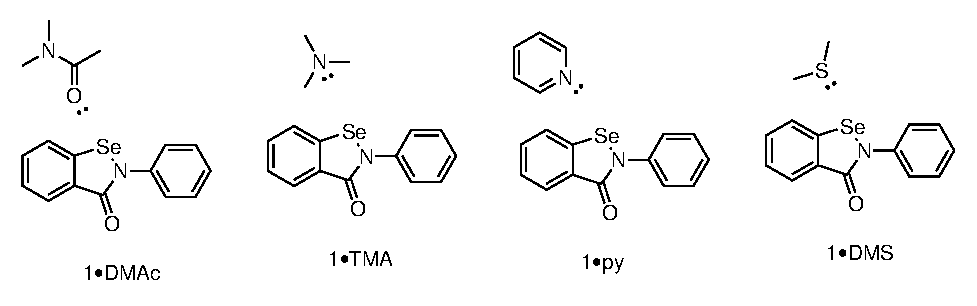
\includegraphics[scale=0.74]{Figures/sapt-complexes.eps}
    \caption{Structures of complexes used for SAPT(DFT) analysis.}
    \label{fig:complexes}
\end{figure}

\begin{figure}
    \centering
    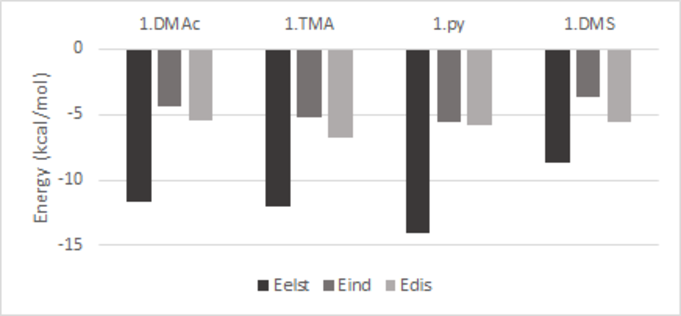
\includegraphics[width=0.5\linewidth]{Figures/sapt-eda.pdf}
    \caption{SAPT(DFT) analysis of complexes with four Lewis bases. All energies are given in kcal/mol.}
    \label{fig:eda}
\end{figure}

The SAPT results indicate that the majority (around 80\%) of the interaction can be described by electrostatics and dispersion.
This suggests that the explicit $\sigma$-hole parametrization will be reliable, as electrostatics and dispersion are well described by MM.

\subsection{Incorporation of pseudoatom}
With classical parameters for ebselen in hand, as well as theoretical assurance that the system can be adequately described using electrostatics, we began to optimize parameters for the pseudoatom representing the $\sigma$-hole.
The pseudoatom was modelled as a virtual site riding on the selenium atom along the extension of the \ce{Se-N} bond.
In GROMACS this is assigned the type \texttt{2fd}, which is described by only one parameter (the distance along the extension of the defining bond).
This very computationally efficient, although it is an approximation to reality, as the center of the $\sigma$-hole is actually slightly offset (see \cref{fig:ebs-esp}).
A more accurate description would be the three-center \texttt{3fd} or \texttt{3fad} type, however this would introduce a performance penalty.

The distance parameter for the pseudoatom was set to 1.189\AA\ which places the point charge on the VdW surface of the selenium atom.
A number of approaches have been suggested to determine this distance, however it is important for numerical stability of the simulation that the charge lies on or within the VdW surface.\autocite{Hobza2012}
The charge of the pseudoatom was calculated using the RESP procedure, which fits a pre-calculated electrostatic potential to atom- (or pseudoatom-) centered point charges while enforcing symmetry restraints.
The ESP was calculated at the HF/6-31G* level using Gaussian16, in order to be consistent with existing force field parameters.
The pseudoatom was then introduced manually, and RESP applied using the ANTECHAMBER program.
For comparison, we also calculated charges for the structure \emph{without} a pseudoatom.
Relevant charges are presented in \cref{tab:charges}, and full library files are available in the supporting information???.

\begin{table}
    \caption{Selected atomic charges for the pseudoatom and no pseudoatom models.}
    \label{tab:charges}
    \begin{tabular}{lll}\toprule
        Atom & RESP charge (pseudoatom) & RESP charge (no pseudoatom) \\\midrule
        \ce{E_{26}} & 0.281382 & --- \\
        \ce{Se_1} & -0.372631 & 0.056728 \\
        \ce{N_2} & -0.241674 & -0.599430 \\
        \ce{C_3} & 0.463064 & 0.827981 \\
        \ce{O_4} & -0.558076 & -0.613468 \\
    \end{tabular}
\end{table}


\subsection{Electrostatic potential map}
With these parameters in hand, we were able to construct electrostatic potential maps (\cref{fig:ebs-esp}), which show good qualitative agreement between the DFT and pseudoatom model potentials.
Barely visible in the DFT ESP map is a second $\sigma$-hole, opposite the Se--C bond.
Carbon is significantly less electronegative than nitrogen, so it doesn't polarize the selenium to the same degree, leading to a much smaller $\sigma$-hole.
While it is conceivable that this $\sigma$-hole could form Ch-bonds as well, we have not observed any evidence of this in any of the derivatives we have studied.\autocite{Fellowes2019}
We therefore did not attempt to model it, although it could be modelled in the same way as the main $\sigma$-hole opposite the nitrogen.

\begin{figure}
    \centering
    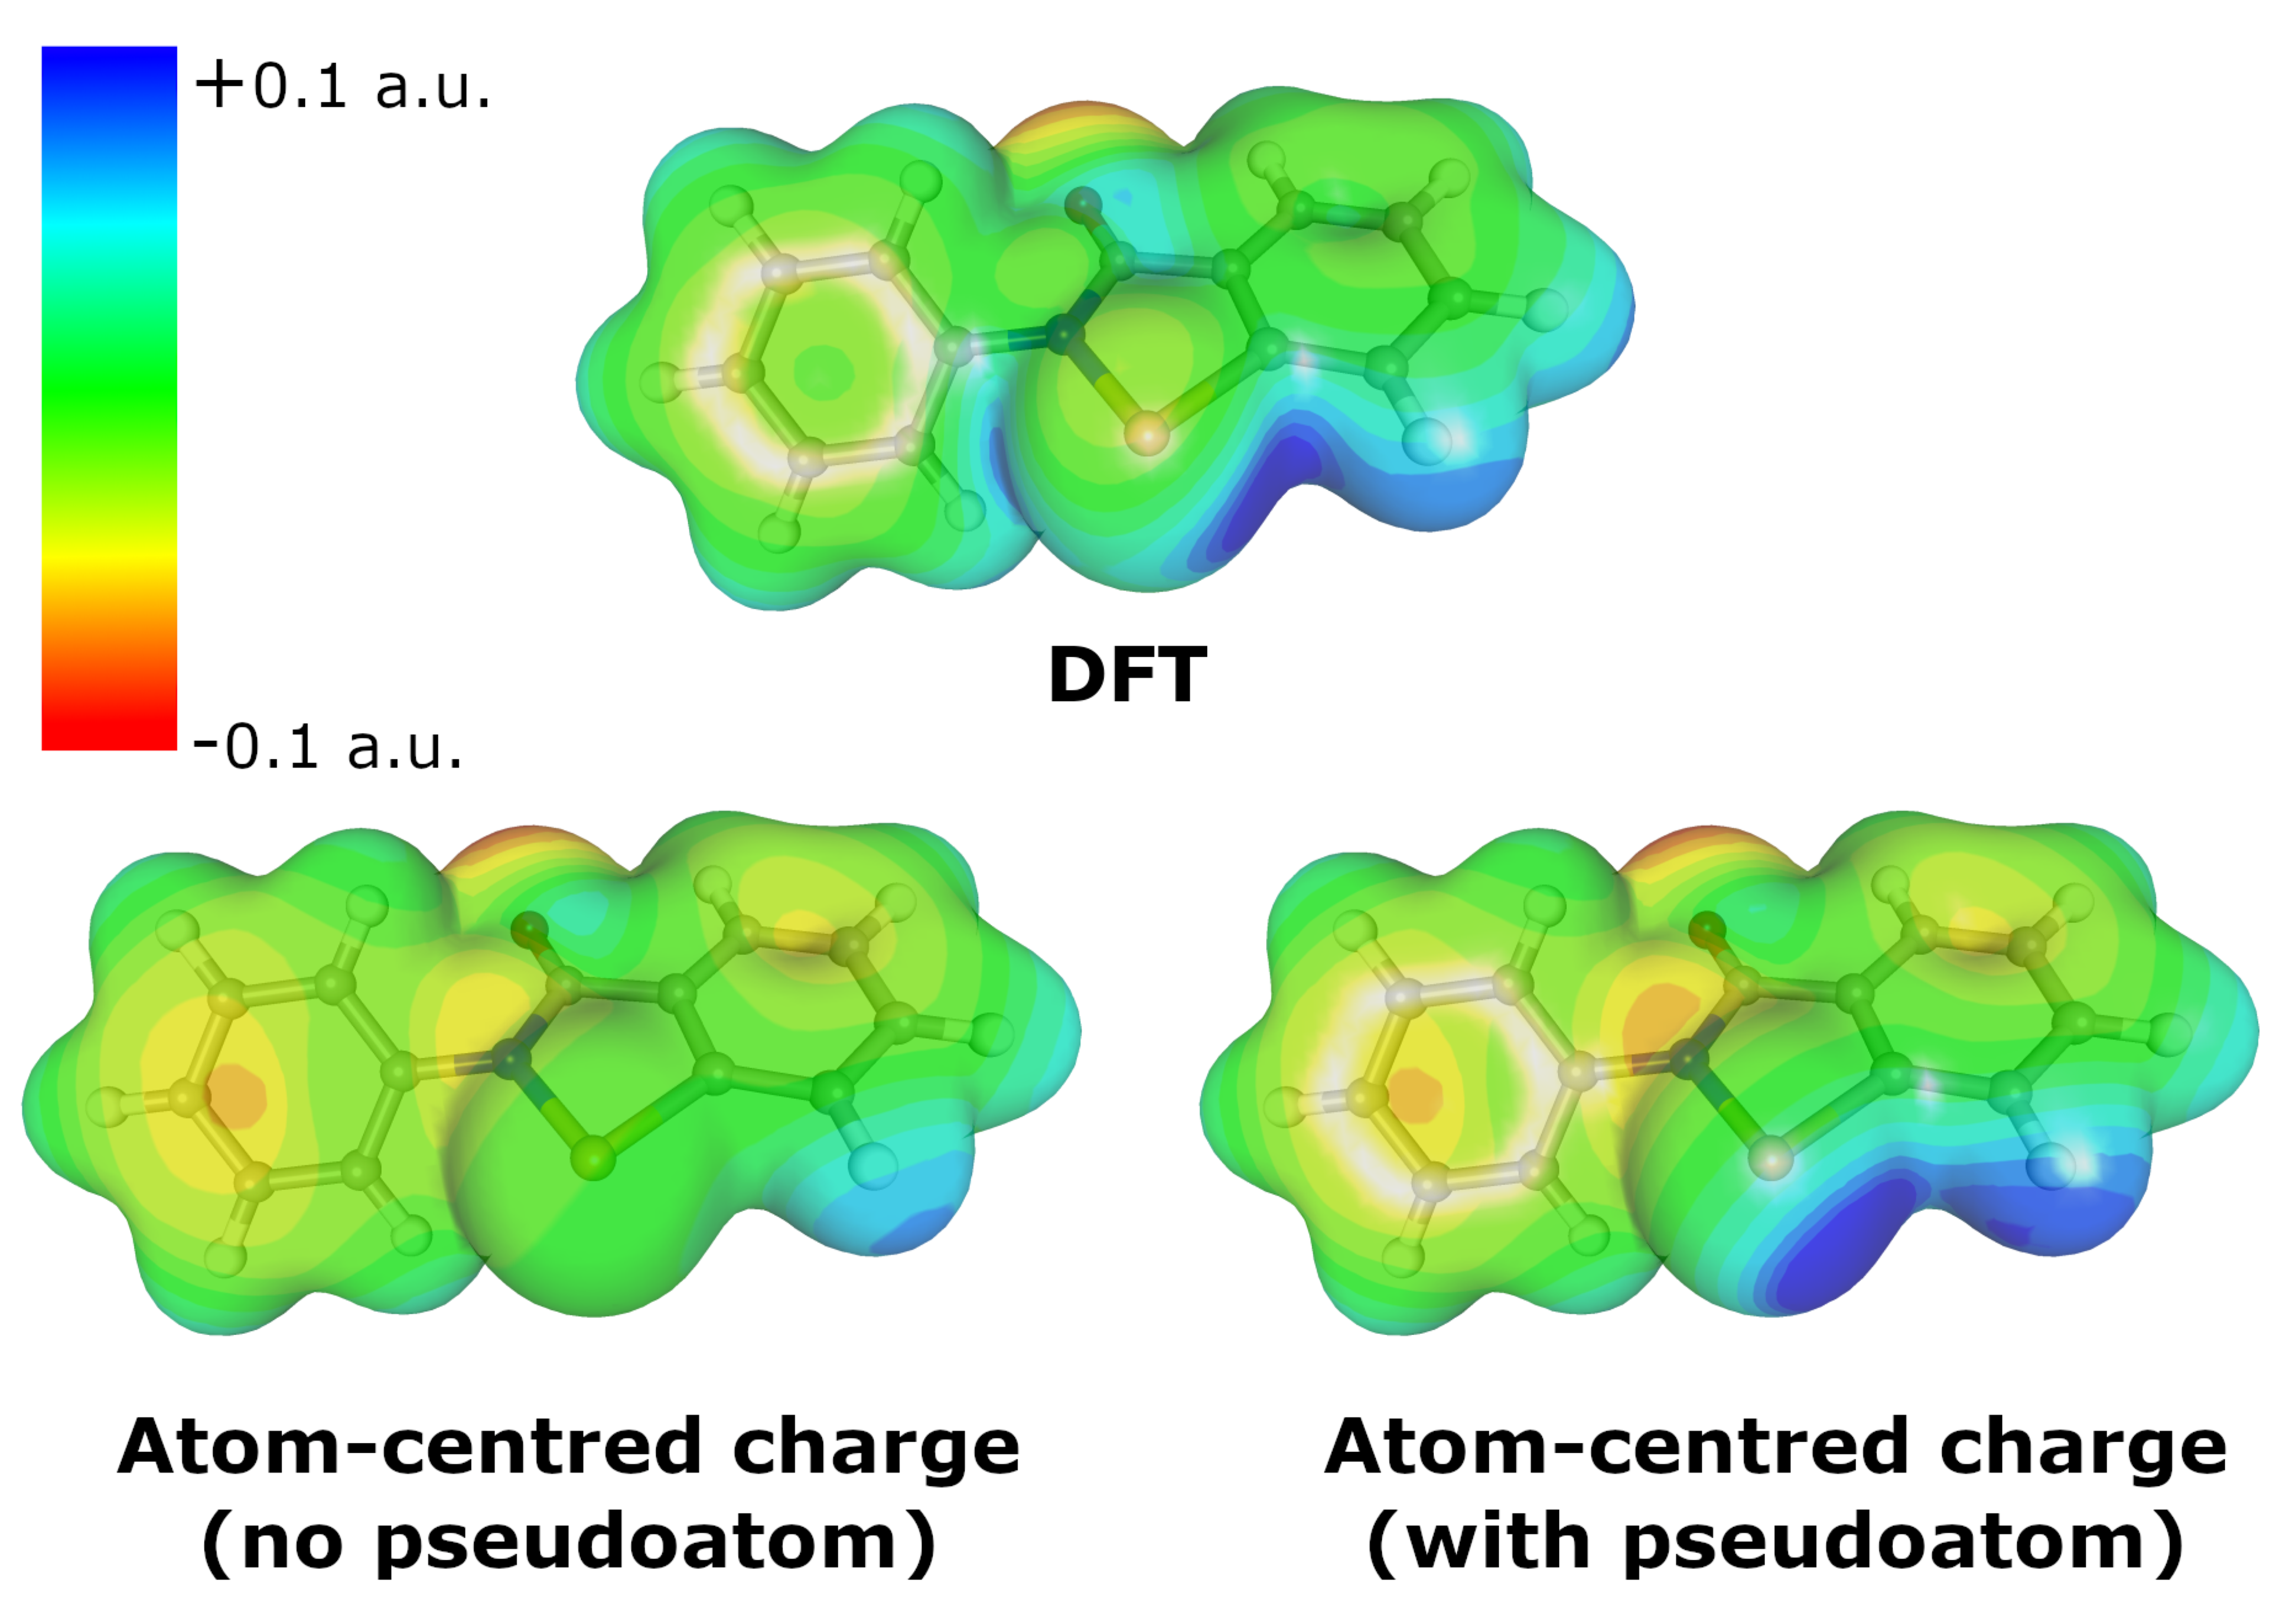
\includegraphics[width=0.5\linewidth]{Figures/mm-dft-esp.pdf}
    \caption{ESP mapped on the 0.005~a.u. electron density isosurface. The $\sigma$-hole is visible as the dark blue region on the DFT and atom-centered charge (with pseudoatom) surfaces.}
    \label{fig:ebs-esp}
\end{figure}

\subsection{Validation against DFT geometries}
A preliminary verification of our model was conducted by comparing the geometries and energies calculated in the SAPT(DFT) analysis with the respective MM values.
The Lewis bases chosen for the SAPT(DFT) analysis were constructed in AMBER.
GAFF was used for all atoms, and an extra point was added to simulate the lone pair per the method of Dixon and Kollman.\autocite{Dixon1997}
Geometries were assessed by minimizing the ebselen-Lewis base structure over 1000 steps, then conducting a 2~ns MD trajectory in a vacuum.
Trajectories were performed at 300~K for the strongly bonded systems (\cmpd{ebs}$\cdot$py and \cmpd{ebs}$\cdot$DMAc), however the weaker complexes (\cmpd{ebs}$\cdot$TMA and \cmpd{ebs}$\cdot$DMS) tended to dissociate under these conditions.
Their trajectories were therefore conducted at 200~K and 100~K respectively.
Binding energies were calculated by slowly cooling the system to 0~K, then conducting a short simulation to determine the potential energy of the system.
Relevant parameters are given in \cref{fig:1.py-geom} and \cref{tab:ebs-geom}, alongside DFT values for comparison.

\begin{figure}
    \centering
    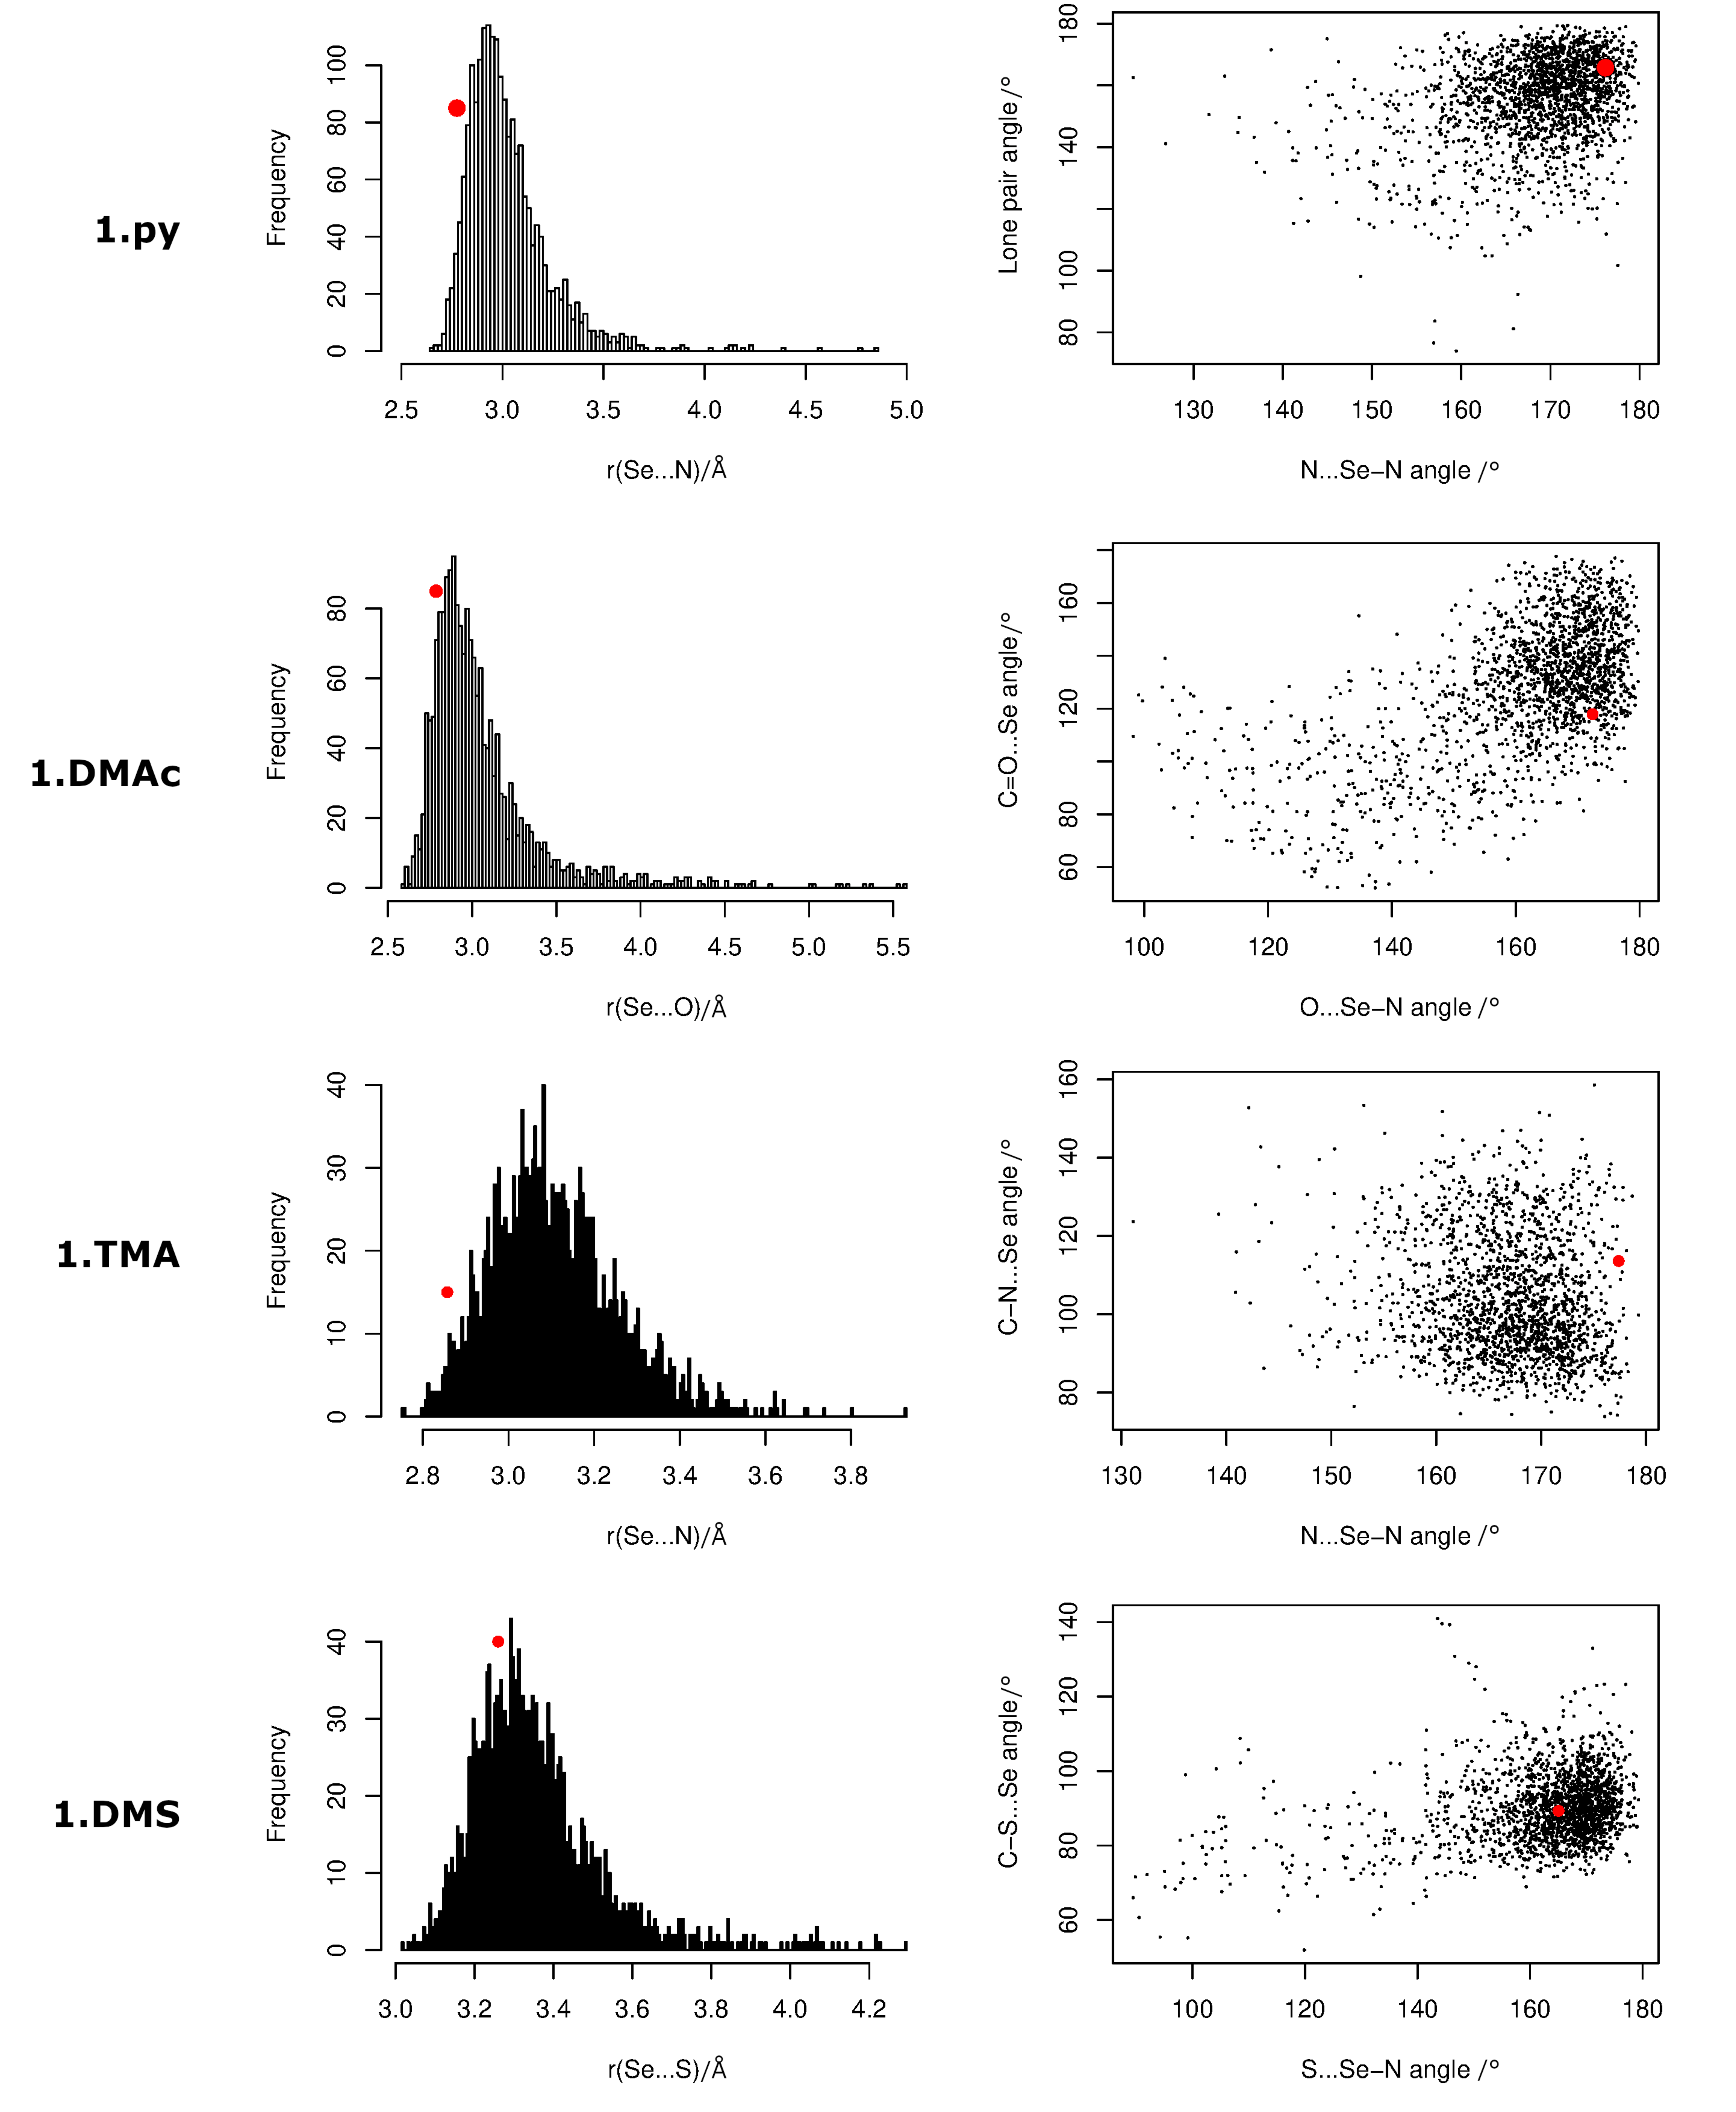
\includegraphics[width=\linewidth]{Figures/geom-distribution.pdf}
    \caption{Distribution of geometric parameters for complexes over a 2~ns trajectory. DFT equilibrium values are shown as red circles.}
    \label{fig:1.py-geom}
\end{figure}

\begin{comment}
    kj/mol
    e ebs =  127.716431
    e tma = -325.562653
    e ebs tma = -220.638214
    e dma = -37.702110
    e ebs dma = 119.586090
    e pyr = -167.397964
    e ebs pyr = -71.262794
    e dms = -47.586956
    e ebs dms = 69.634117
\end{comment}

\begin{table}
    %DONE
    \centering
    \begin{tabular}{lllll}\toprule
        Complex & r(\ce{Se\cdots B}) & $\angle$(\ce{N-Se\cdots B}) & $\angle$(lone pair) & Energy \\ & & & & (kcal/mol)\\\midrule
        \cmpd{ebs}$\cdot$py & 2.879~\AA~(2.775~\AA) & 174.9\degree~(176.2\degree) & 171.1\degree~(165.7\degree) & -7.548 (-7.093) \\%DONE
        \cmpd{ebs}$\cdot$DMAc & 2.741~\AA~(2.786~\AA) & 174.7\degree~(172.4\degree) & 129.1\degree~(117.9\degree) & -7.068 (-7.551) \\%DONE
        \cmpd{ebs}$\cdot$TMA & 2.928~\AA~(2.857~\AA) & 170.1\degree~(177.4\degree) & 107.2\degree~(113.6\degree) & -5.447 (-6.627) \\%DONE
        \cmpd{ebs}$\cdot$DMS & 3.253~\AA~(3.265~\AA) & 160.4\degree~(177.4\degree) & 81.2\degree~(89.8\degree) & -2.510 (-5.646) \\%DONE
        \bottomrule
    \end{tabular}
    \caption{Median geometric parameters for complexes with \cmpd{ebs}. DFT equilibrium values are given in brackets for comparison. DFT energies are derived from SAPT(DFT).}
    \label{tab:ebs-geom}
\end{table}

These results show that Ch-bonds can be adequately described by the inclusion of a positively charged pseudoatom.
Almost all parameters and energies can be adequately reproduced, with the only anomaly being the substantially underestimated bond energy for the \cmpd{ebs}$\cdot$DMS complex.
Interestingly, the geometry is modelled well in spite of this.
This may be due to the increased role of dispersion in this complex, which has been deliberately de-emphasised in our parameters in order to emulate the polar flattening of the selenium.
There is also a substantial charge-transfer component to this interaction which, when taken to completion, leads to formation of a \ce{Se-S} bond and opening of the ring (\cref{fig:catcycle}).
This cannot be modelled in a harmonic force field, so it is perhaps not surprising that the interaction energy is underestimated.
Nonetheless, we believe that the parameter set will still be very useful for molecular docking.

\subsection{Validation against experimental melting point}
We also sought to validate our model against the experimentally determined melting point.
An ebselen crystal (CSD code \textbf{SENGOH}, $5 \times 5 \times 5$ unit cells, 1000 molecules) was constructed, and placed in a simulation box of the appropriate size at 1~atm.
The crystal was heated to 300K, then 5 random molecules were deleted to create voids (crystal defects) that act as nucleation sites for melting.
This avoids the effects of superheating, which is a documented issue in simulated phase transitions.\autocite{???}
The nucleated geometry was used as a starting point for a series of trajectories at temperatures from 400--500~K in 10~K increments to identify an approximate melting range, then 1~K increments to accurately determine the melting point.

\begin{figure}
    \centering
    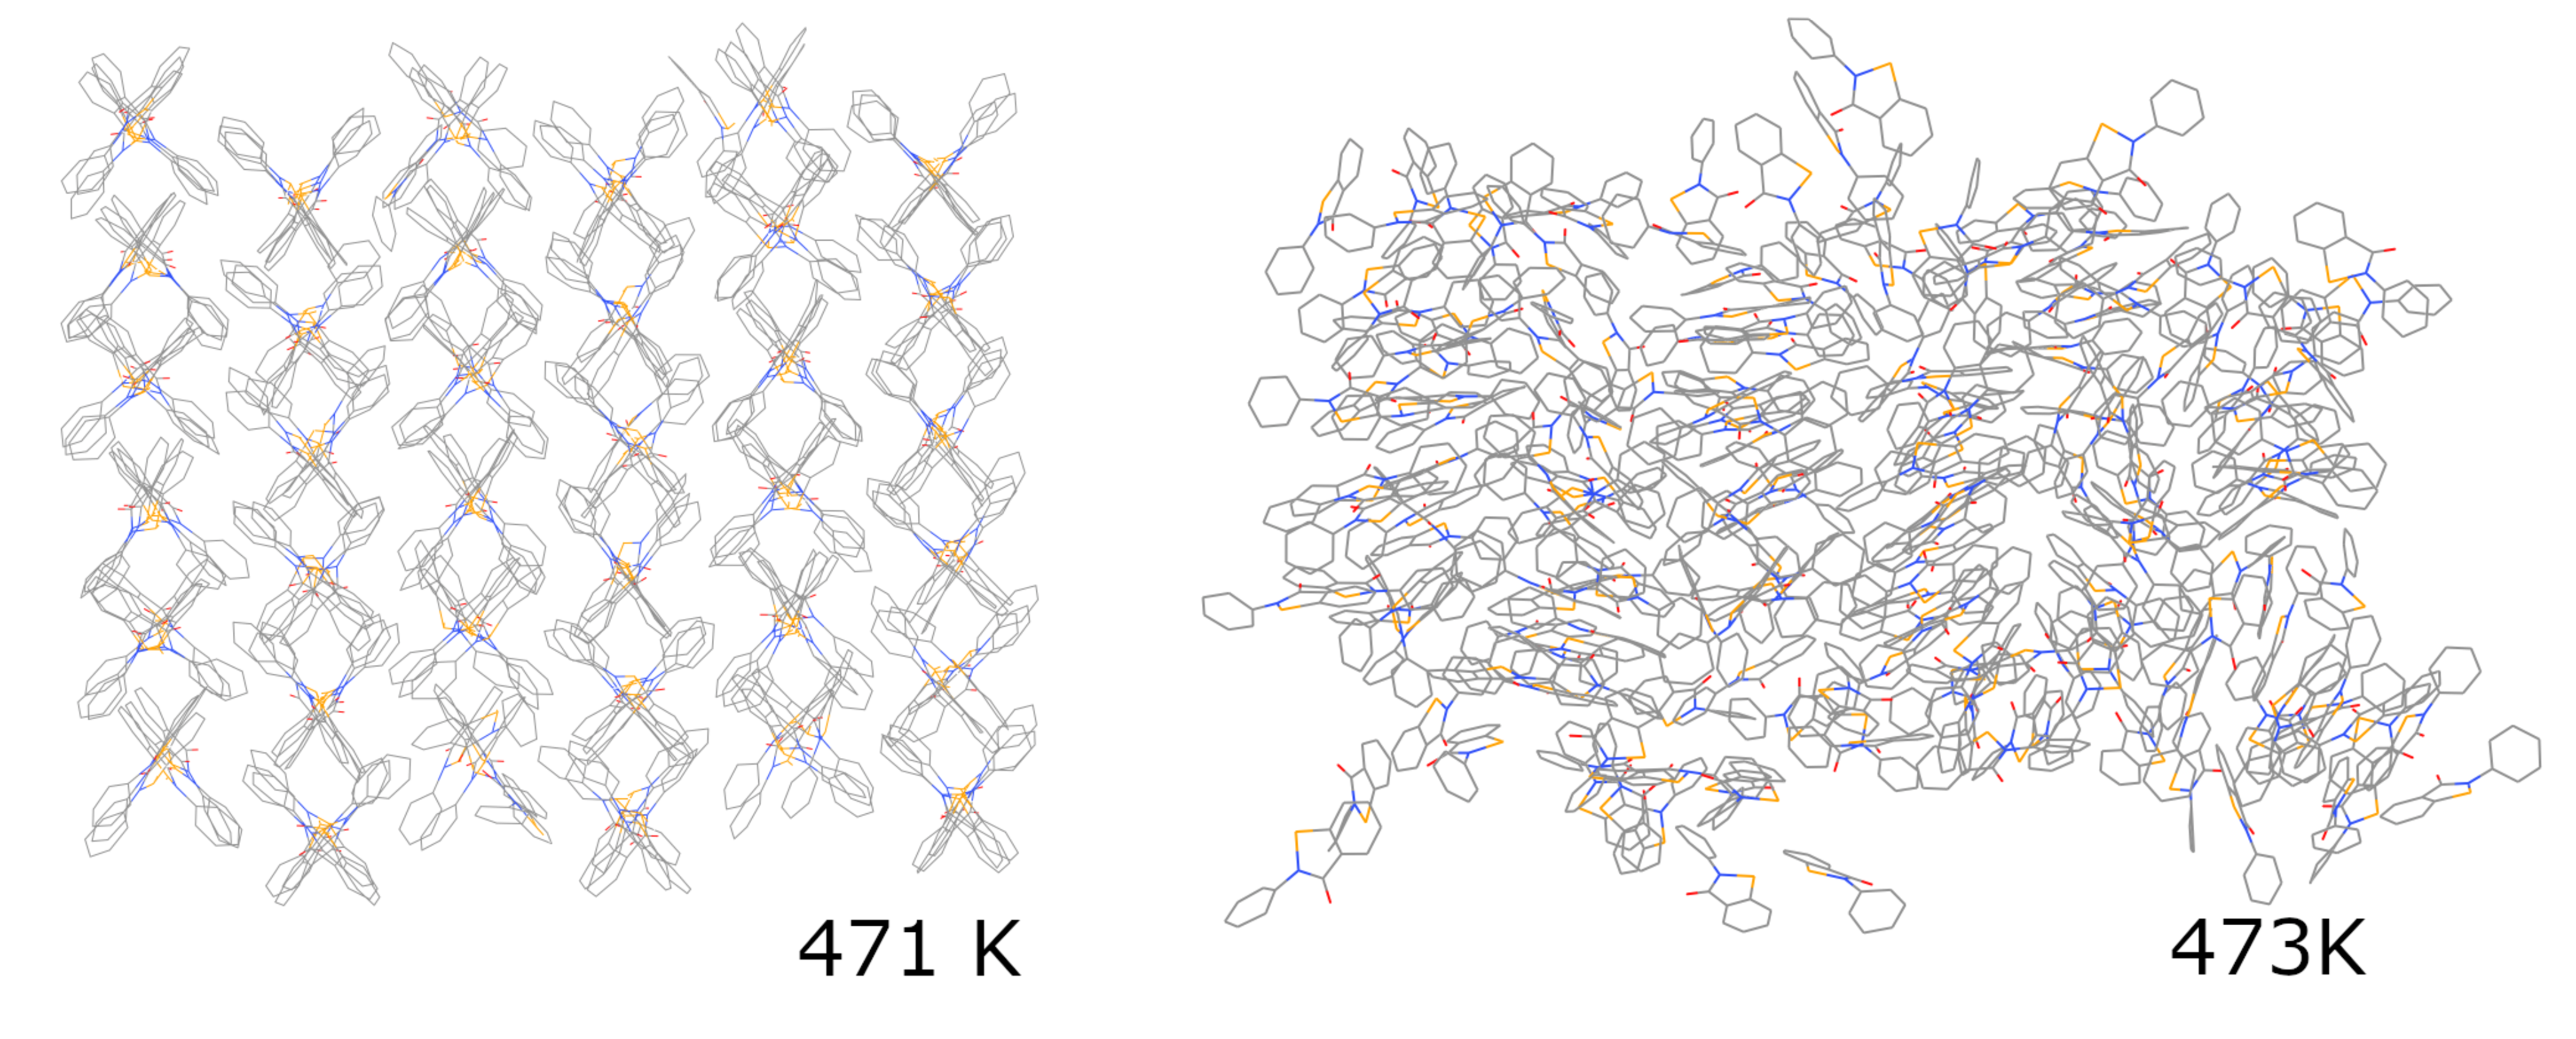
\includegraphics[width=\columnwidth]{Figures/melting.pdf}
    \caption{Melting of a simulated ebselen crystal. The final state of the crystal is shown after 2~ns at the specified temperature.}
    \label{fig:melting}
\end{figure}



\subsection{Validation against SOD1 binding}
In order to show the utility of our model, we conducted a binding simulation with a known ebselen target.
Superoxide dismutase-1 (SOD1) forms a covalent complex with ebselen through the Cys111 residue, which appears to support correct folding of the protein, inhibiting aggregation and associated toxicity.\autocite{Capper2018}
Although formation of the covalent complex cannot be simulated using our model (as this is a bond-forming process), we are able to visualize the stabilized encounter complex which undergoes ring opening to form the final adduct.
Indeed, the Ch-bond formed through the $\sigma$-hole can be thought of as the early stages of a nucleophilic attack at the selenium.\autocite{Thomas2015}
SOD1 (PDB \textbf{2C9V}) was chosen because of the availability of an atomic resolution structure, demonstrated evidence of ebselen binding, and it's relatively small size.\autocite{Capper2018,Strange2006}
The structure was prepared for AMBER by removing disorder, then removing water and ions (the Cu and Zn ions were retained).
The ff14SB force field was used for the protein.
The ebselen residue was introduced within the binding groove approximately halfway between the two units.
The complex was then neutralized by addition of four \ce{Na+} ions at the sites of most negative electrostatic potential, and solvated with a TIP3P explicit water model to give a final box size of $77.095\times 96.253\times 78.411$\AA.
The structure was minimized over 1000 cycles to remove bad contacts, then heated to 300~K over 200~ps.
A simulation of 2~ns at 300~K was then performed to assess the average binding geometry, which was found to exhibit a bifurcated Ch-bond between the expected Cys111 sulfur and the adjacent Ile113 backbone carbonyl (\cref{fig:sod1-ebs}).
A similar experiment was performed \emph{without} the $\sigma$-hole, which failed to bind in a reproducible geometry, with the ebselen molecule wandering through the groove.
This is presumably driven by hydrophobic interactions, and the entropic cost of desolvation.

\begin{figure}
    \centering
    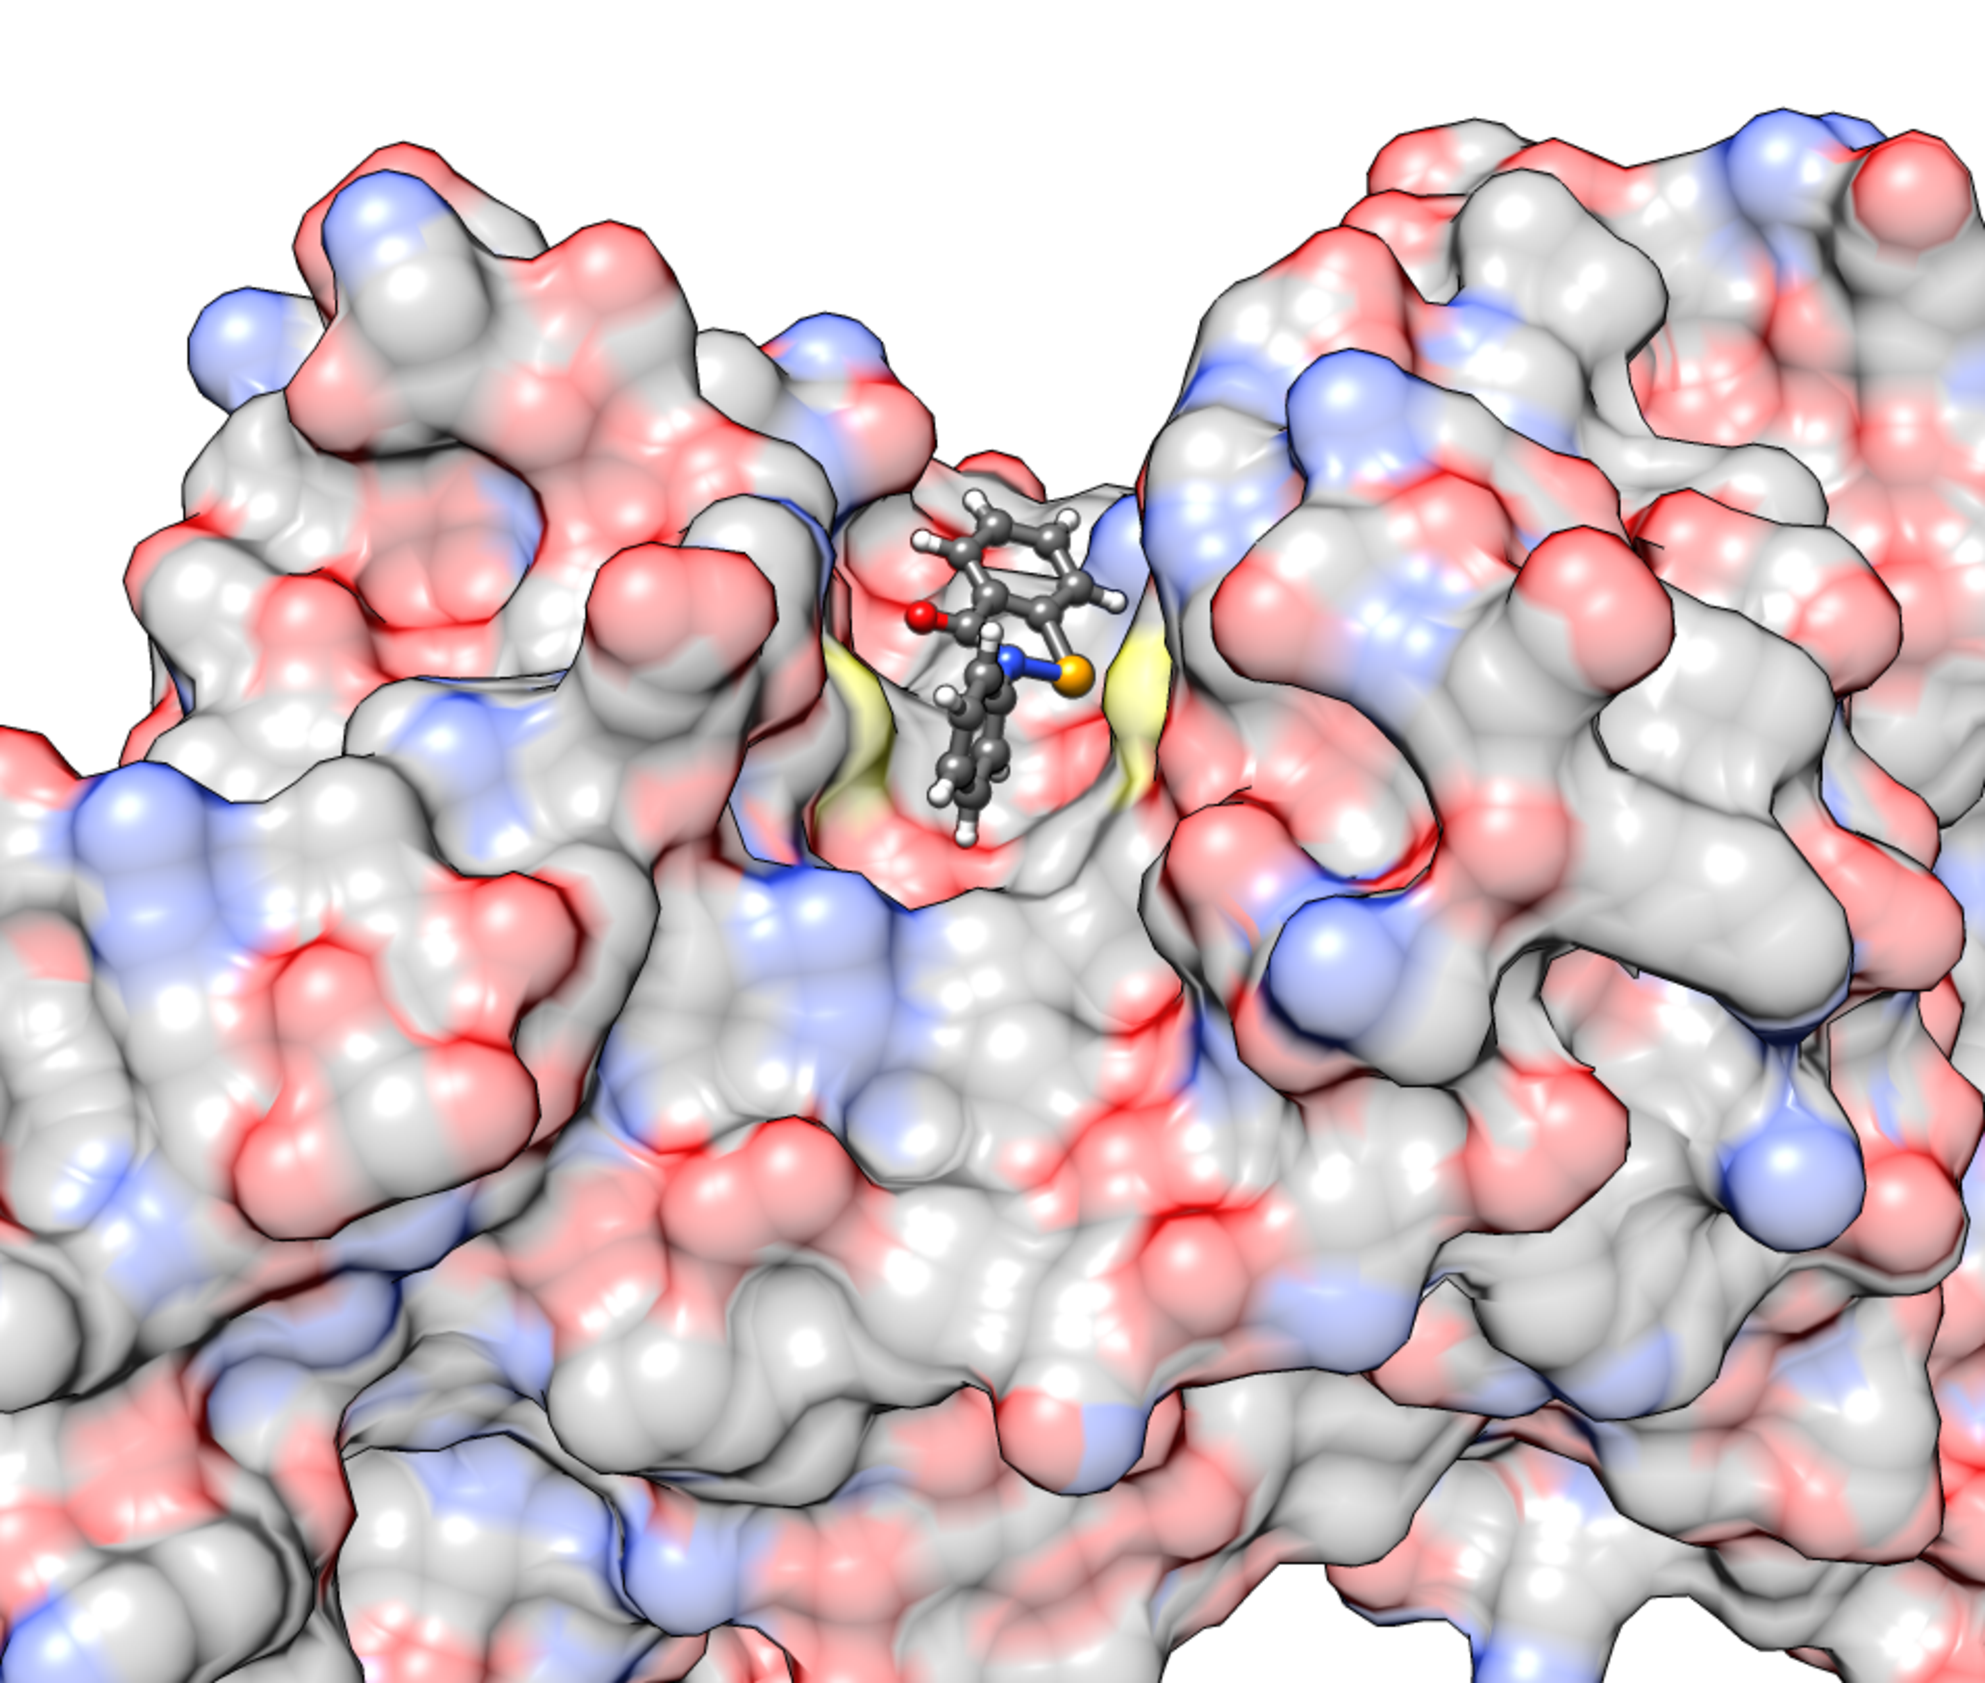
\includegraphics[width=0.45\linewidth]{Figures/sod1-ebs-a.pdf}
    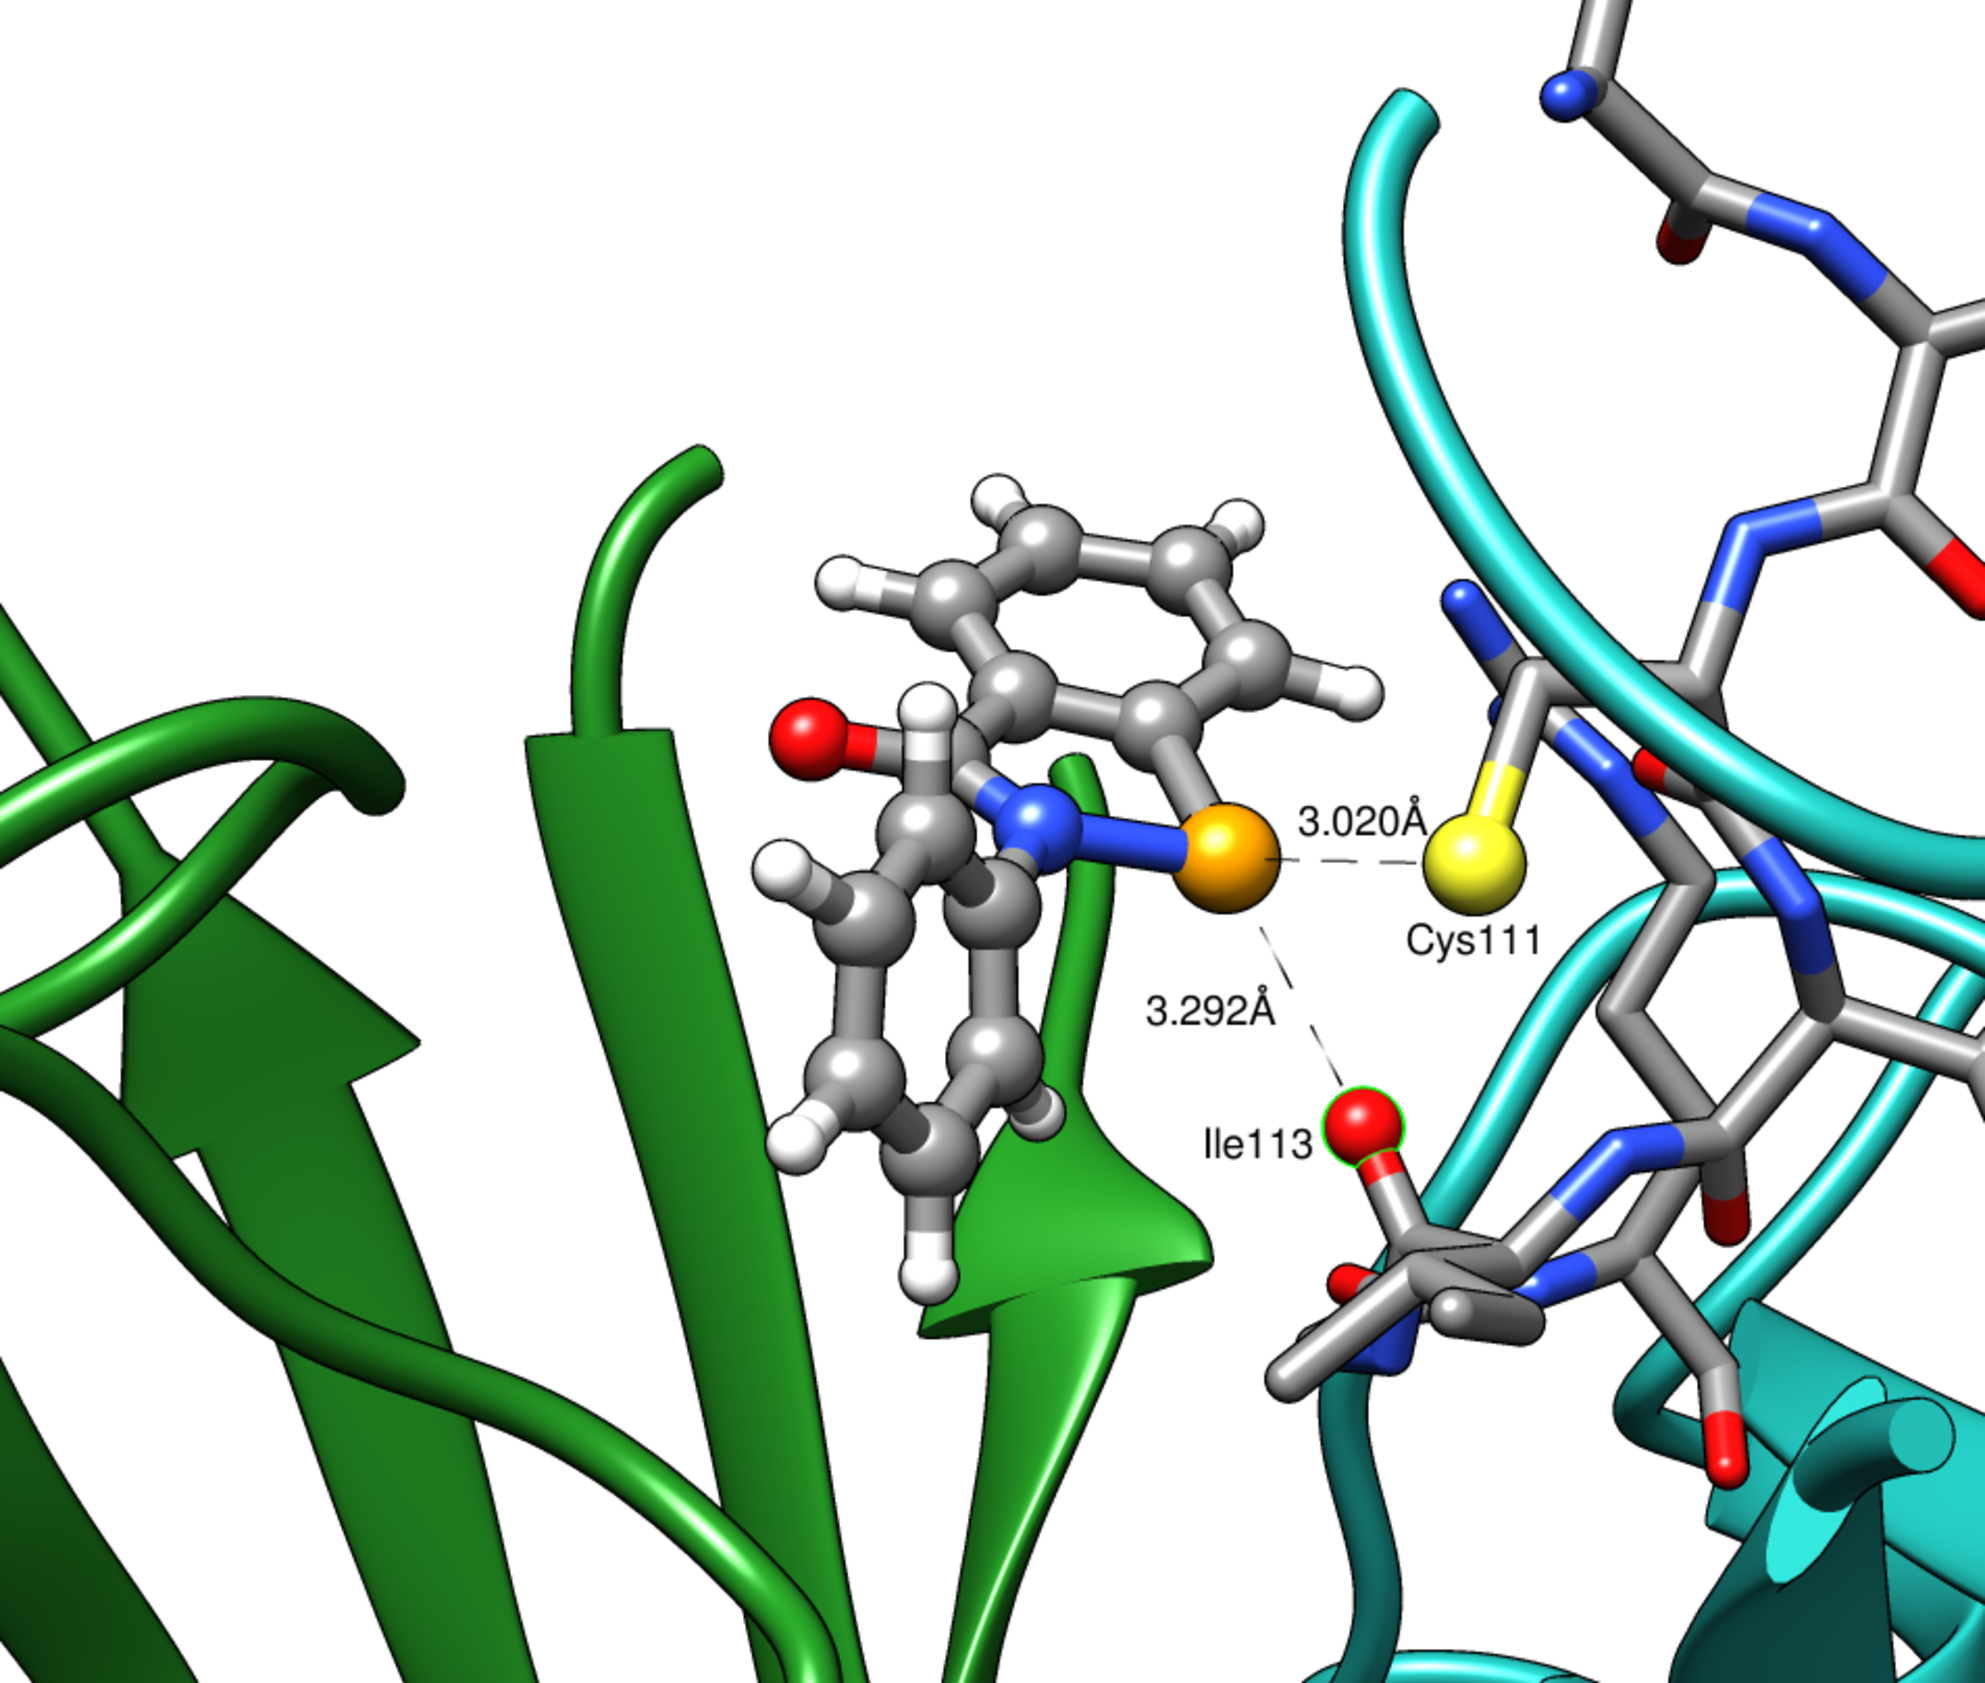
\includegraphics[width=0.45\linewidth]{Figures/sod1-ebs-b.pdf}
    \caption{Average binding geometry of ebselen in the SOD1 groove.}
    \label{fig:sod1-ebs}
\end{figure}

\section{Conclusion}
In conclusion, we have developed a set of parameters which can greatly improve modelling of ebselen and its derivatives.
Our model gives realistic geometries and energies of gas phase complexes, and reproduces the interaction between ebselen and a protein.
Although this work is restricted to ebselen itself, the parameters will be generally applicable to derivatives of ebselen (with appropriate charge fitting).
We hope that these results will be useful for the discovery of new targets.

\printbibliography[heading=subbibliography]
\end{refsection}


\part{The strength and nature of chalcogen bonding}
 
\begin{refsection}

\chapter[Insights from co-crystal structures]{New insights into chalcogen bonding provided by co-crystal structures of benzisoselenazolinone derivatives and nitrogen bases.}

This chapter was published in Cryst. Eng. Comm., 22 Jan 2019\autocite{Fellowes2019}. \footnote{Compound numbering, section headings, and terminology have been updated to fit this thesis.}

\section{Abstract}
A number of derivatives of benzisoselenazolinones, including the drug ebselen, have been synthesized, and their interactions with various nitrogen bases characterized through x-ray crystallography.
Structural studies revealed a strong interaction in all cases, with Se$\cdots$N distances well within the Van der Waals radii of the constituent atoms.
We suggest that there is a significant charge transfer component to this interaction, in contrast to some other interactions of similar strength and directionality.
We have also found that this interaction can be enhanced \emph{via} H-bonding to the carbonyl group of the benzisoselenazolinone moiety.

\cmpd*{ebs.ph}
\cmpd*{ebs.bn}
\cmpd*{ebs.h}
\cmpd*{amide.ph}
\cmpd*{amide.bn}
\cmpd*{amide.h}
\cmpd*{tetracycle}

\section{Introduction}
Chalcogen bonding (Ch-bonding) is a class of non-covalent interaction which has recently piqued the interests of the chemical community, and potential applications in materials and medicinal chemistry are emerging.\autocite{Mitchell2017,Wonner2017a,Fanfrlik2014,Vogel2019}
It bears similarities to the related concept of halogen bonding, and the ubiquitous phenomenon of hydrogen bonding, in that the result is a relatively strong and highly directional non-bonded interaction.\autocite{Paolo1974}
This strength and directionality has been exploited in crystal engineering\autocite{Gleiter2003,Kremer2016,Huynh2017}, anion recognition\autocite{Lim2017,Lim2018,Garrett2016}, and bond activation \autocite{Wonner2017,Benz2017,Benz2017a}, and appears to play a critical role in protein folding\autocite{Iwaoka2001,Iwaoka2015}.
Studies on Te$\cdots$N Ch-bonds in solution phase have shown they can be as strong as 2.7~kcal/mol\autocite{Garrett2015a}.
A number of interesting and potentially useful supramolecular polymers have been synthesised and characterised by Vargas-Baca \emph{et al}, based on tellurium- and selenium-containing heterocycles\autocite{Ho2016,Ho2017}.

In our efforts to apply the concept of Ch-bonding to biological systems, we turned to the benzisoselenazolinone scaffold of the antioxidant compound ebselen \cmpd{ebs.ph}.
\cmpd{ebs.ph} has been known since the 1980s to effectively scavenge reactive oxygen species \emph{in vivo}.\autocite{Muller1984}
It has remarkably low toxicity for an organoselenium compound, and is being investigated as a possible treatment for a number of conditions.\autocite{Schewe1995,Kil2007,Singh2013,Parnham2000}
It is also an ideal scaffold for Ch-bonding, bearing a selenium atom bonded to an electronegative amide nitrogen.
Indeed, Ch-bonding in \cmpd{ebs.ph} has been investigated previously in the context of crystal packing of the pure compound, but there is a lack of experimental evidence for interactions with other acceptors.\autocite{Thomas2015}

Numerous studies have examined the nature of the Ch-bond, in particular the balance between electrostatic effects (due to anisotropic electrostatic potential around the chalcogen atom), covalent (orbital overlap and electron delocalisation), and dispersion forces.\autocite{Oliveira2017,Pascoe2017,DeVleeschouwer2017,Kolar2016,Gleiter2018}
In the case of halogen bonding, these contributions are generally well characterized.
Halogen bonds range from primarily electrostatic (as in the case of fluorinated iodobenzenes\autocite{Prasang2009}) to charge-transfer dominated (molecular halogens\autocite{Mulliken1950}).
In the case of Ch-bonding in derivatives of \cmpd{ebs.ph}, the contributions are less clear.
We therefore sought to characterize Ch-bonding interactions between a number of derivatives of \cmpd{ebs.ph}, and a variety of Ch-bond acceptors.

\begin{figure}
  \centering
  \replacecmpd[sub-only]{amide.ph}
  \replacecmpd[sub-only]{amide.bn}
  \replacecmpd[sub-only]{amide.h}
  \replacecmpd{tetracycle}
  \replacecmpd{ebs.{ph,bn}}
  \replacecmpd{amide.{ph,bn,h}}
  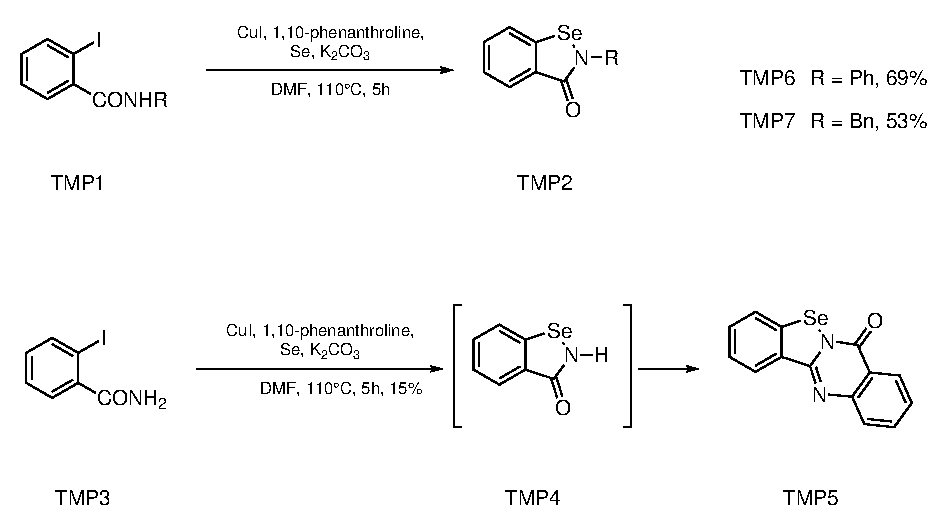
\includegraphics[scale=0.8]{Figures/catalytic-synthesis.eps}
  \caption{Synthesis of Ch-bond donors \refcmpd{ebs.ph}, \refcmpd{ebs.bn} and \refcmpd{tetracycle}.}
  \label{fig:synthesis}
\end{figure}

\section{Results and Discussion}
\subsection{Synthesis of benzisoselenazolone derivatives \refcmpd{ebs.ph,ebs.bn}}
Compounds \cmpd{ebs.ph} and \cmpd{ebs.bn} were synthesized via published procedures from amides \cmpd{amide.ph} and \cmpd{amide.bn}.\autocite{Bhabak2010}
The Se-tetracycle \cmpd{tetracycle} was isolated in poor yield as the major product from the cyclization of primary amide \cmpd{amide.h} in an attempt to form \cmpd{ebs.h}.
It is noteworthy that the spectral characteristics of \cmpd{tetracycle} are essentially identical to reported spectral data of \cmpd{ebs.h}\autocite{Bhabak2010}.

\begin{table}
  \centering
  \caption{Selected structural parameters of Ch-bonded complexes}
  \tablefit{\begin{tabular}{lllllll}
    \toprule
    Complex & r(N$\cdots$Se) & r(Se--N\textsubscript{1}) & r(Se--C\textsubscript{1}) & r(N\textsubscript{1}--C(O)) & $\angle$(N$\cdots$Se--N\textsubscript{1}) & $\angle$(C\textsubscript{para}$\cdots$N$\cdots$Se) \\
      & \AA\ & \AA\ & \AA\ & \AA\ & $^\circ$ & $^\circ$ \\ \midrule
    \cmpd{ebs.ph} only & --- \\
    \cmpd{ebs.ph} $\cdot$ DMAP & 2.371(1) & 1.9676(10) & 1.8959(12) & 1.2345(14) & 174.18(4) & 173.52(4) \\
    \cmpd{ebs.bn} only & --- & 1.8805(14) & 1.8867(16) & 1.350(2) & --- & --- \\
    \cmpd{ebs.bn} $\cdot$ DMAP M1 & 2.4276(14) & 1.9297(13) & 1.8984(15) & 1.348(2) & 173.93(5) & 174.89(5) \\
    \cmpd{ebs.bn} $\cdot$ DMAP M2 & 2.4331(14) & 1.9191(14) & 1.8966(14) & 1.349(2) & 175.30(5) & 158.14(5) \\
    \cmpd{ebs.bn} $\cdot$ DMAP $\cdot$ \ce{H2O} & 2.4046(15) & 1.9367(14) & 1.9070(14) & 1.330(2) & 175.54(5) & 167.43(5) \\
    \cmpd{ebs.bn} $\cdot$ quinuclidine & 2.5874(17) & 1.9077(17) & 1.898(2) & 1.354(3) & 176.77(7) & 161.32(7) \\
    \cmpd{ebs.bn} $\cdot$ DABCO & 2.6166(15) & 1.9019(14) & 1.8967(17) & 1.355(2) & 175.76(6) & 160.00(6) \\
    \cmpd{tetracycle} only & --- & 1.883(2) & 1.899(3) & 1.393(3) & --- & --- \\
    \cmpd{tetracycle} $\cdot$ pyridine & 2.461(3) & 1.926(2) & 1.908(3) & 1.373(4) & 174.13(9) & 169.1(1)\\
    \cmpd{tetracycle} $\cdot$ DMAP & 2.304(1) & 1.9716(9) & 1.918(1) & 1.375(1) & 173.81(4) & 173.16(4) \\
    \bottomrule
    \end{tabular}}
  \label{tab:bondlengths}
\end{table}

\section{Co-crystal structures of benzisoselenazolinones and Lewis bases}
High quality low temperature crystal structures were obtained for the parent benzisoselenazolinone derivatives \cmpd{ebs.ph} \autocite{Thomas2015}, \cmpd{ebs.bn} and the Se-tetracycle \cmpd{tetracycle} and the chalcogen-bonded co-crystals of these compounds with a variety of nitrogen bases, including pyridine, dimethylaminopyridine (DMAP) quinuclidine and DABCO.
Powder diffaction patterns were obtained of the bulk co-crystal material and compared with the single crystal data, with excellent agreement.
This provides strong evidence of phase purity, with the exception of \cmpd{ebs.bn}$\cdot$DMAP, which indicated the presence of the unbound monomers in addition to the Ch-bonded adduct.
Relevant structural parameters are presented in \cref{tab:bondlengths}, while all thermal ellipsoid plots are presented in the supplementary material (SUPP-Figures 7--15$^\dag$).
In the following discussion we begin by assessing the Ch-bond donor abilities of \cmpd{ebs.ph}, \cmpd{ebs.bn}, and \cmpd{tetracycle} by comparing the structural parameters with a common nitrogen base adduct (DMAP), followed by comparison of a single Ch-bond donor \cmpd{tetracycle} with two different nitrogen bases with markedly different basicities (pyridine and DMAP).

\subsection{Effects of the benzisoselenazolone on Ch-bond strength}
The DMAP adducts of \cmpd{ebs.ph}, \cmpd{ebs.bn} and \cmpd{tetracycle} are characterized by near linear N$\cdots$Se--N(CO) angles (\cref{tab:bondlengths}) with N\textsubscript{DMAP}$\cdots$Se distances which are 2.4276(14) and 2.4331(16)~\AA \ for the two independent molecules of \cmpd{ebs.bn}, 2.371(1)~\AA\ for \cmpd{ebs.ph}, and the strikingly short N$\cdots$Se distance of 2.304(1)~\AA\ for \cmpd{tetracycle}.
All are well within the van der Waals radii of N and Se of 3.85~\AA\ \autocite{Batsanov2001}.
The antipodal Se--N\textsubscript{1} bond distance within these adducts is significantly lengthened compared to the free Ch-bond donors, 0.063~\AA\ in \cmpd{ebs.ph}, 0.049~\AA\ in \cmpd{ebs.bn}, and 0.088~\AA\ in \cmpd{tetracycle}, with the degree of lengthening being related in an inverse sense to the N\textsubscript{DMAP}$\cdots$Se distance, in all cases the (non-antipodal) Se--C\textsubscript{1} bond is essentially unchanged.
These structural parameters suggest an order of Ch-bond donor abilities \cmpd{ebs.bn} < \cmpd{ebs.ph} < \cmpd{tetracycle}, which is supported by theoretical calculations which are discussed below, as well as being consistent with the \textsuperscript{77}Se NMR chemical shifts.

\subsection{Endocyclic bond lengthening associated with stronger complexes}
Further discussion is warranted on the \cmpd{ebs.bn}$\cdot$DMAP adduct.
Firstly, the two independent molecules of \cmpd{ebs.bn}$\cdot$DMAP differ significantly with respect to the direction that the nitrogen base lone pair makes with the Se--N\textsubscript{1} bond.
In molecule 1 this angle is close to colinear at 174.89(5)$^\circ$ while in molecule 2, this deviates significantly from linearity 158.14(5)$^\circ$.
Associated with this difference is a slightly longer N\textsubscript{DMAP}$\cdots$Se distance of 2.4331(14)~\AA\ in molecule 2 compared to 2.4276(14)~\AA\ in molecule 1 ($\Delta$=0.0055~\AA ; 3$\sigma$) and a shorter Se--N\textsubscript{1} distance 1.9191(14)~\AA\ vs 1.9297(14)~\AA\ ($\Delta$=-0.10~\AA ; 7.5$\sigma$) indicating a slightly weaker interaction.
This can be seen in \cref{fig:benzyl-dmap-xray-2}.

\begin{figure}
  \centering
  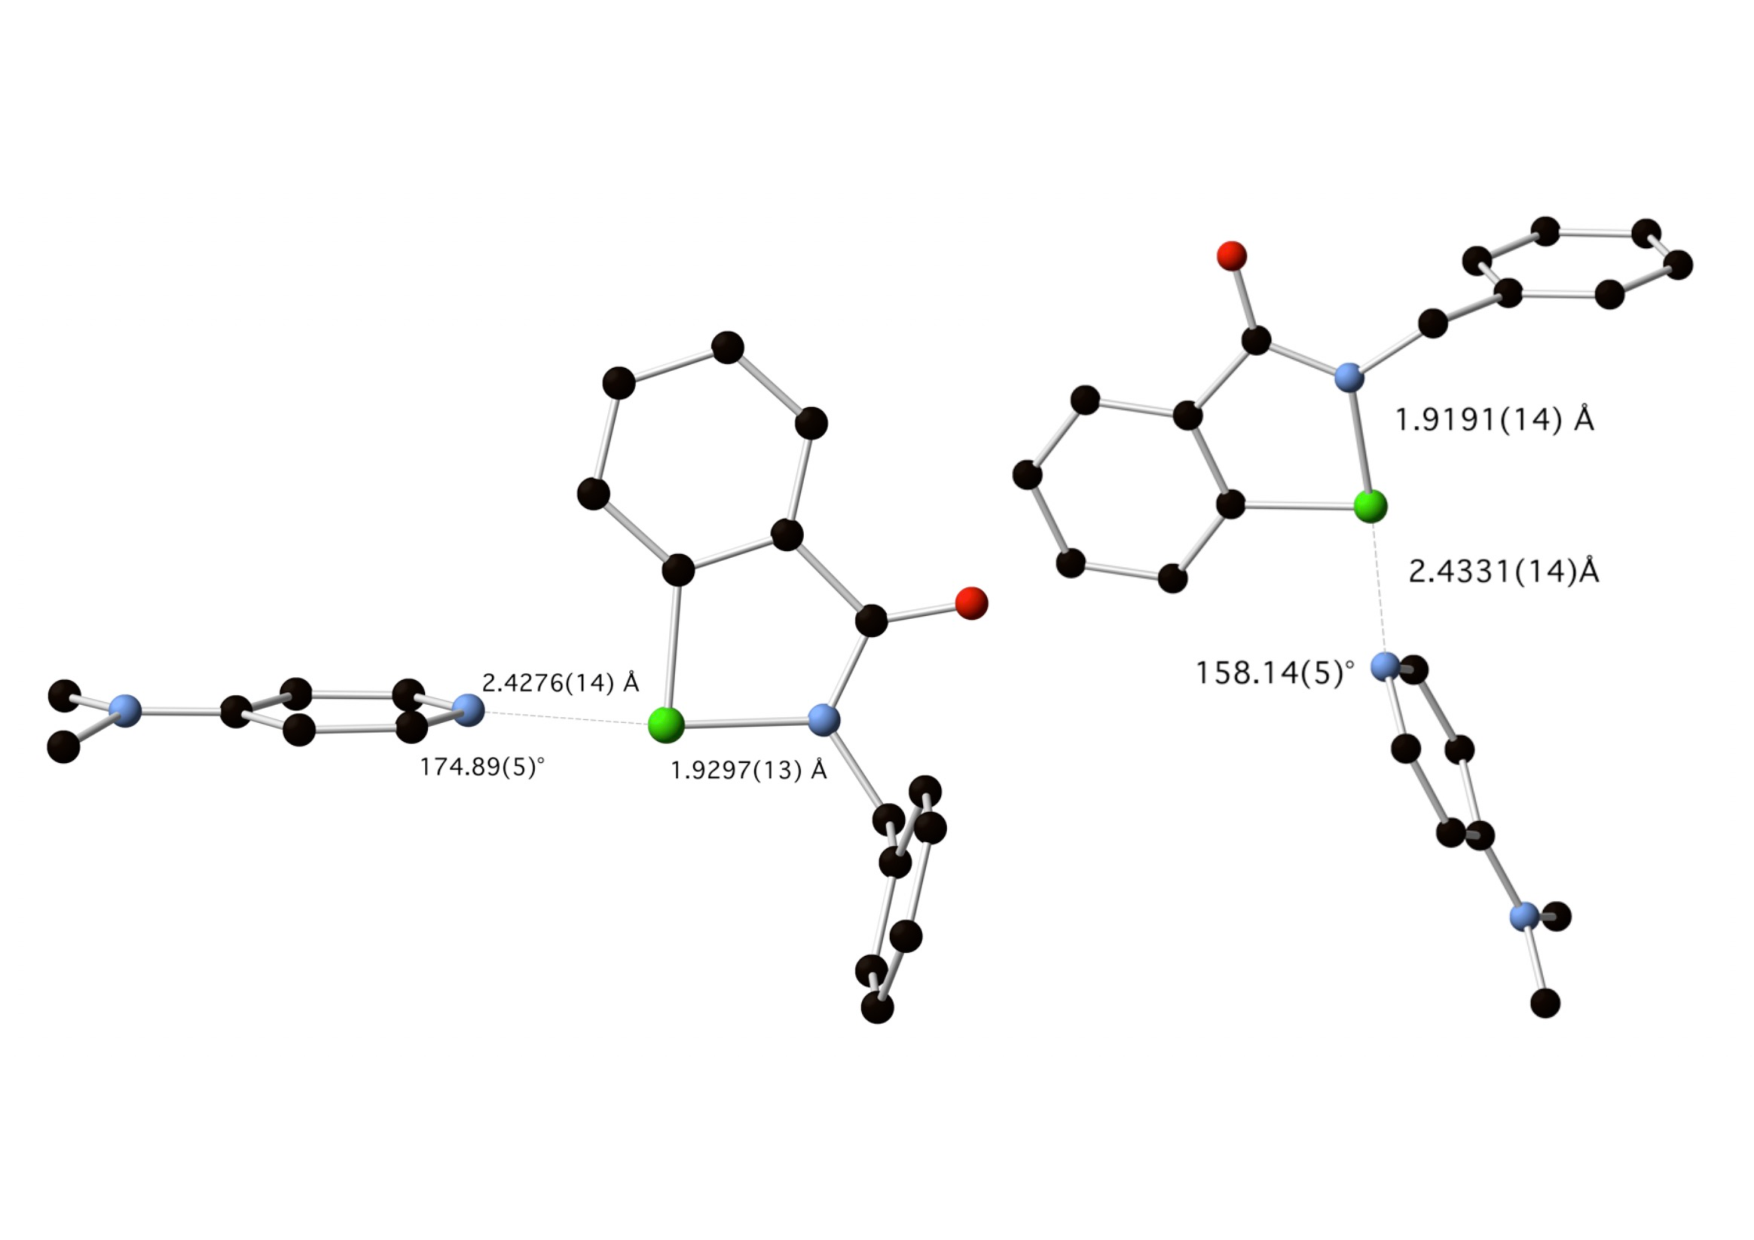
\includegraphics[width=0.8\linewidth]{Figures/benzyl-dmap-xray-2.pdf}
  \caption{Structure of \refcmpd{ebs.bn}$\cdot$DMAP, showing the two distinct geometries.}
  \label{fig:benzyl-dmap-xray-2}
\end{figure}

The structural effects described, particularly the lengthening of the Se--N\textsubscript{1} bond are consistent with donation of electron density from the nitrogen lone pair into the Se--N\textsubscript{1} antibonding orbital being a significant component of these N$\cdots$Se Ch-bonds, which has been described before\autocite{Pascoe2017}.

\subsection{H-bond enhanced Ch-bonding}
The second reason for further discussion of the \cmpd{ebs.bn}$\cdot$DMAP adduct is based on the structural parameters obtained for the hydrate structure \cmpd{ebs.bn}$\cdot$DMAP$\cdot$\ce{H2O} which was serendipitously obtained by evaporation of a THF solution in an open flask.
The structure is shown in \cref{fig:benzyl-dmap-hydrate}.

\begin{figure}
  \centering
  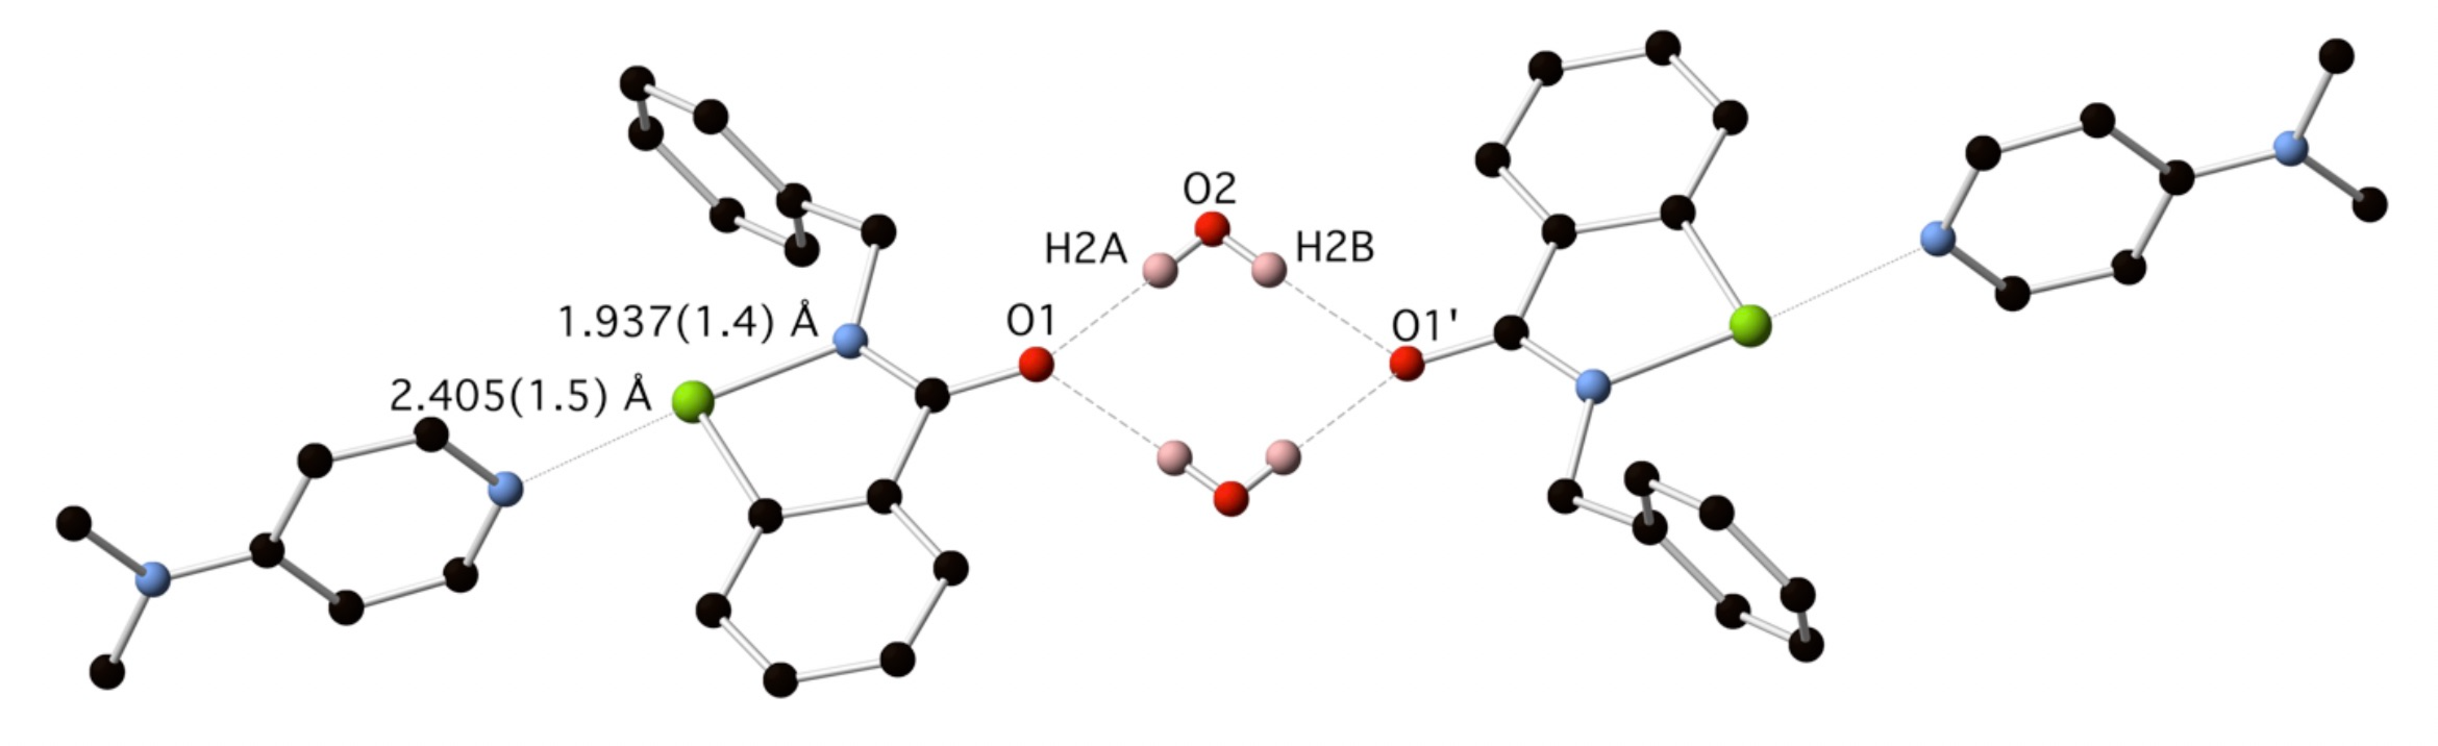
\includegraphics[width=0.8\linewidth]{Figures/benzyl-dmap-hydrate.pdf}
  \caption{Structure of \refcmpd{ebs.bn}$\cdot$DMAP$\cdot$\ce{H2O}.}
  \label{fig:benzyl-dmap-hydrate}
\end{figure}

\cmpd{ebs.bn}$\cdot$DMAP$\cdot$\ce{H2O} crystallizes as a centrosymmetric hydrogen-bonded dimer in which two water molecules bridge two molecules of \cmpd{ebs.bn} across a crystallographic inversion centre.
Of note, when comparison is made between the structural parameters for \cmpd{ebs.bn}$\cdot$DMAP molecule 1, which has a similar geometry about the N$\cdots$Se moiety as for \cmpd{ebs.bn}$\cdot$DMAP$\cdot$\ce{H2O}, there is a significant contraction of the N\textsubscript{DMAP}$\cdots$Se distance from 2.4276(14)~\AA\ to 2.4046(14)~\AA\ ($\Delta$=-0.023~\AA ; 16$\sigma$), and an increase in the Se--N\textsubscript{1} bond distance from 1.9297(13) to 1.9367(14)~\AA\ ($\Delta$=0.007~\AA ; 5$\sigma$).
We have coined the term `hydrogen-bond enhanced Ch-bonding' to describe this interesting structural effect.

\subsection{Effects of the Lewis base on Ch-bond strength}
We were fortunate to obtain crystal structures of the Se-tetracycle \cmpd{tetracycle} with both pyridine and DMAP, which gave us the opportunity to compare the structural effects arising from two Ch-bond acceptors with significantly different basicities.
The pyridine adduct of \cmpd{tetracycle} is characterized by a N\textsubscript{PYR}$\cdots$Se distance 2.461(3)~\AA\ and Se--N\textsubscript{1} distance of 1.926(2)~\AA\ and a near linear N\textsubscript{PYR}$\cdots$Se--N\textsubscript{1} angle, the Se--N\textsubscript{1} bond distance is significantly longer than the corresponding distance 1.883(2)~\AA\ in non-bound structure of \cmpd{tetracycle}.
The DMAP adduct of \cmpd{tetracycle} is characterized by a significantly shorter N\textsubscript{DMAP}$\cdots$Se distance of 2.304(1)~\AA\ ($\Delta$=-0.157~\AA) and longer Se--N\textsubscript{1} distance of 1.9716(9)~\AA\ ($\Delta$=0.046~\AA), consistent with a significantly stronger interaction.

\begin{figure}
  \centering
  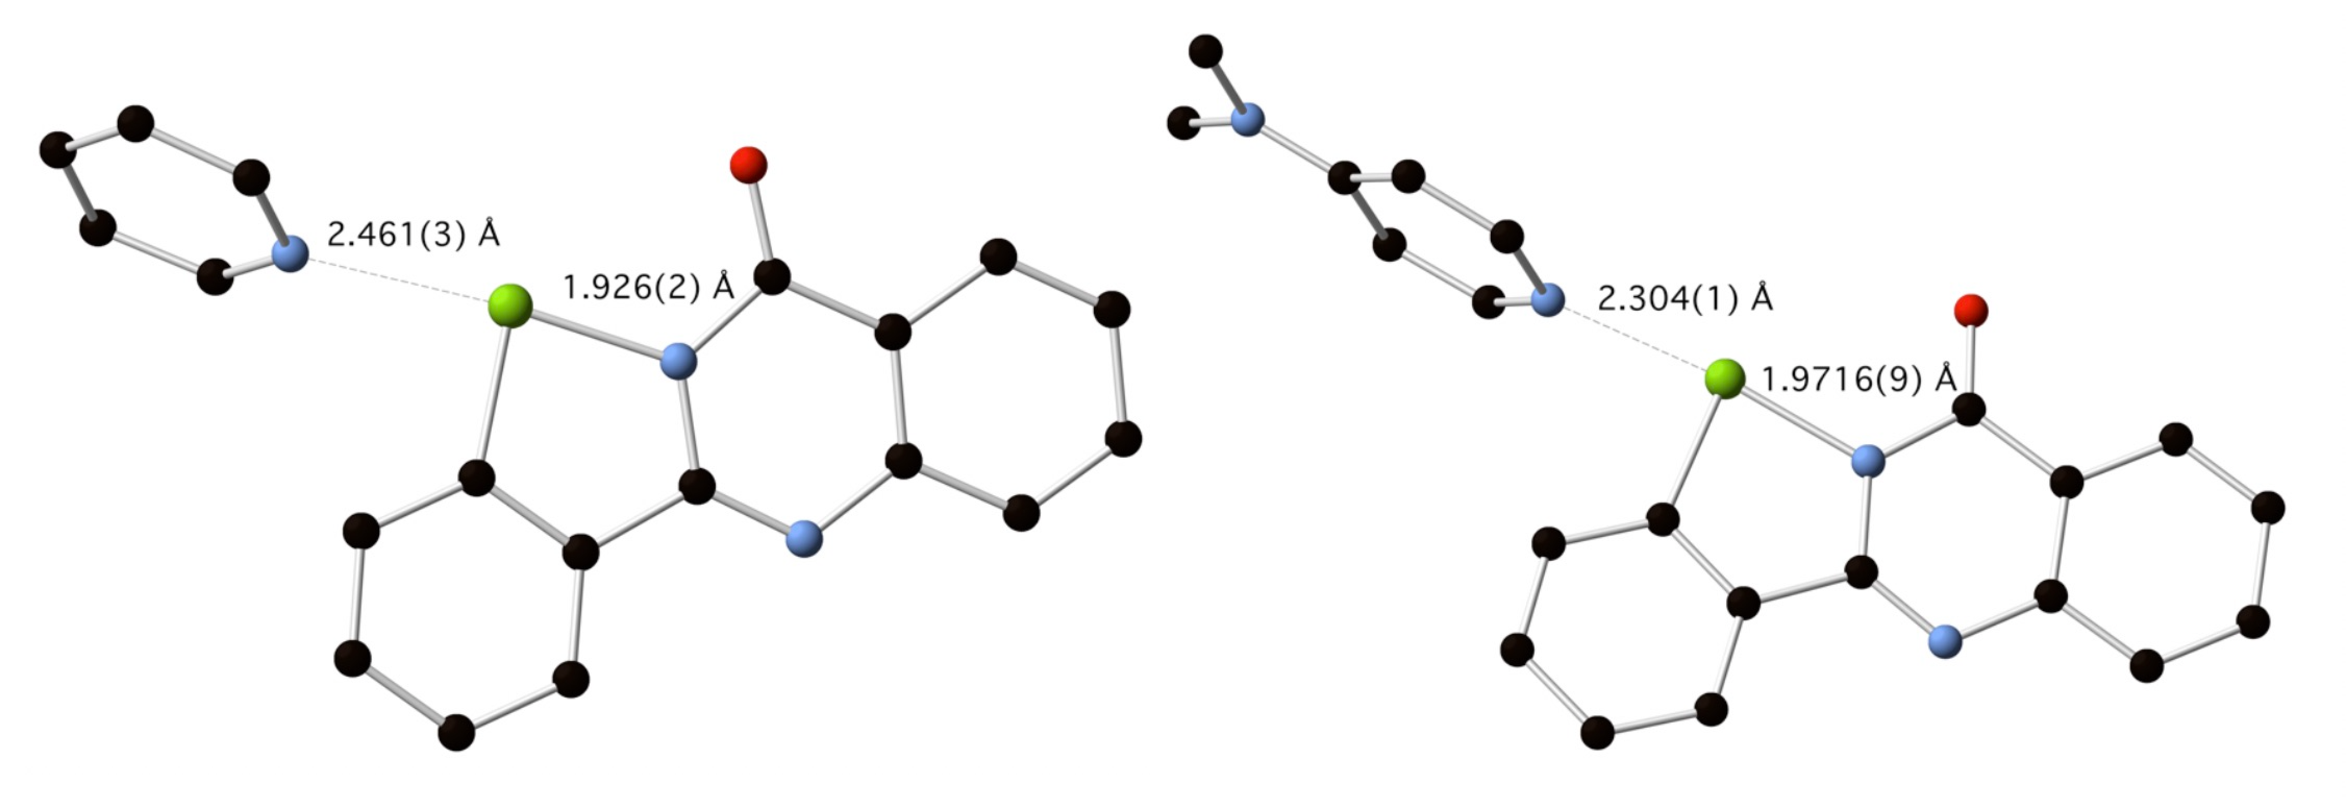
\includegraphics[width=0.8\linewidth]{Figures/dimer-dmap-py-xray.pdf}
  \caption{Pyridine and DMAP adducts of Se-tetracycle \refcmpd{tetracycle}.}
  \label{fig:dimer-adducts}
\end{figure}

Ch-bonded co-crystals of the benzisoselenazolinone derivative \cmpd{ebs.bn} with the tertiary amines; quinuclidine and DABCO were obtained and structurally characterized.
The adducts are presented in \cref{fig:benzyl-adducts}.
The N\textsubscript{QUIN}$\cdots$Se and N\textsubscript{DABCO}$\cdots$Se distances of 2.5874(17)~\AA\ and 2.6166(15)~\AA\ for \cmpd{ebs.bn}$\cdot$quinuclidine and \cmpd{ebs.bn}$\cdot$DABCO respectively are significantly longer than those observed for \cmpd{ebs.bn}$\cdot$DMAP suggesting an order of Ch-bond strengths with \cmpd{ebs.bn} DABCO < Quinuclidine < DMAP which correlates well with the hydrogen bond acceptor ability of these bases, as quantified by the pK\textsubscript{HB} (\cref{tab:pkhb}).

\begin{table}
  \centering
  \caption{Hydrogen bond basicities of bases studied.}
  \begin{tabular}{lllll}
    \toprule
                            & pyridine                      & DABCO                     & quinuclidine              & DMAP \\\midrule
      pK\textsubscript{HB}  & 1.86\autocite{Berthelot1998}  & 2.63\autocite{Graton2002} & 2.71\autocite{Graton2002} & 2.80\autocite{Berthelot1998}\\
      \cmpd{ebs.bn}$\cdot$base r(N$\cdots$Se) / \AA & ---   & 2.6166(15)                & 2.5874(17)                & 2.4276(14)\footnote{Bond distance given is the shorter of the two coordination environments.}\\
      \cmpd{ebs.bn}$\cdot$base $\Delta$H\textsubscript{f} / kcal/mol & -6.35    & -7.82 & ---                       & -7.91\\\bottomrule
  \end{tabular}
  \label{tab:pkhb}
\end{table}

\begin{figure}
  \centering
  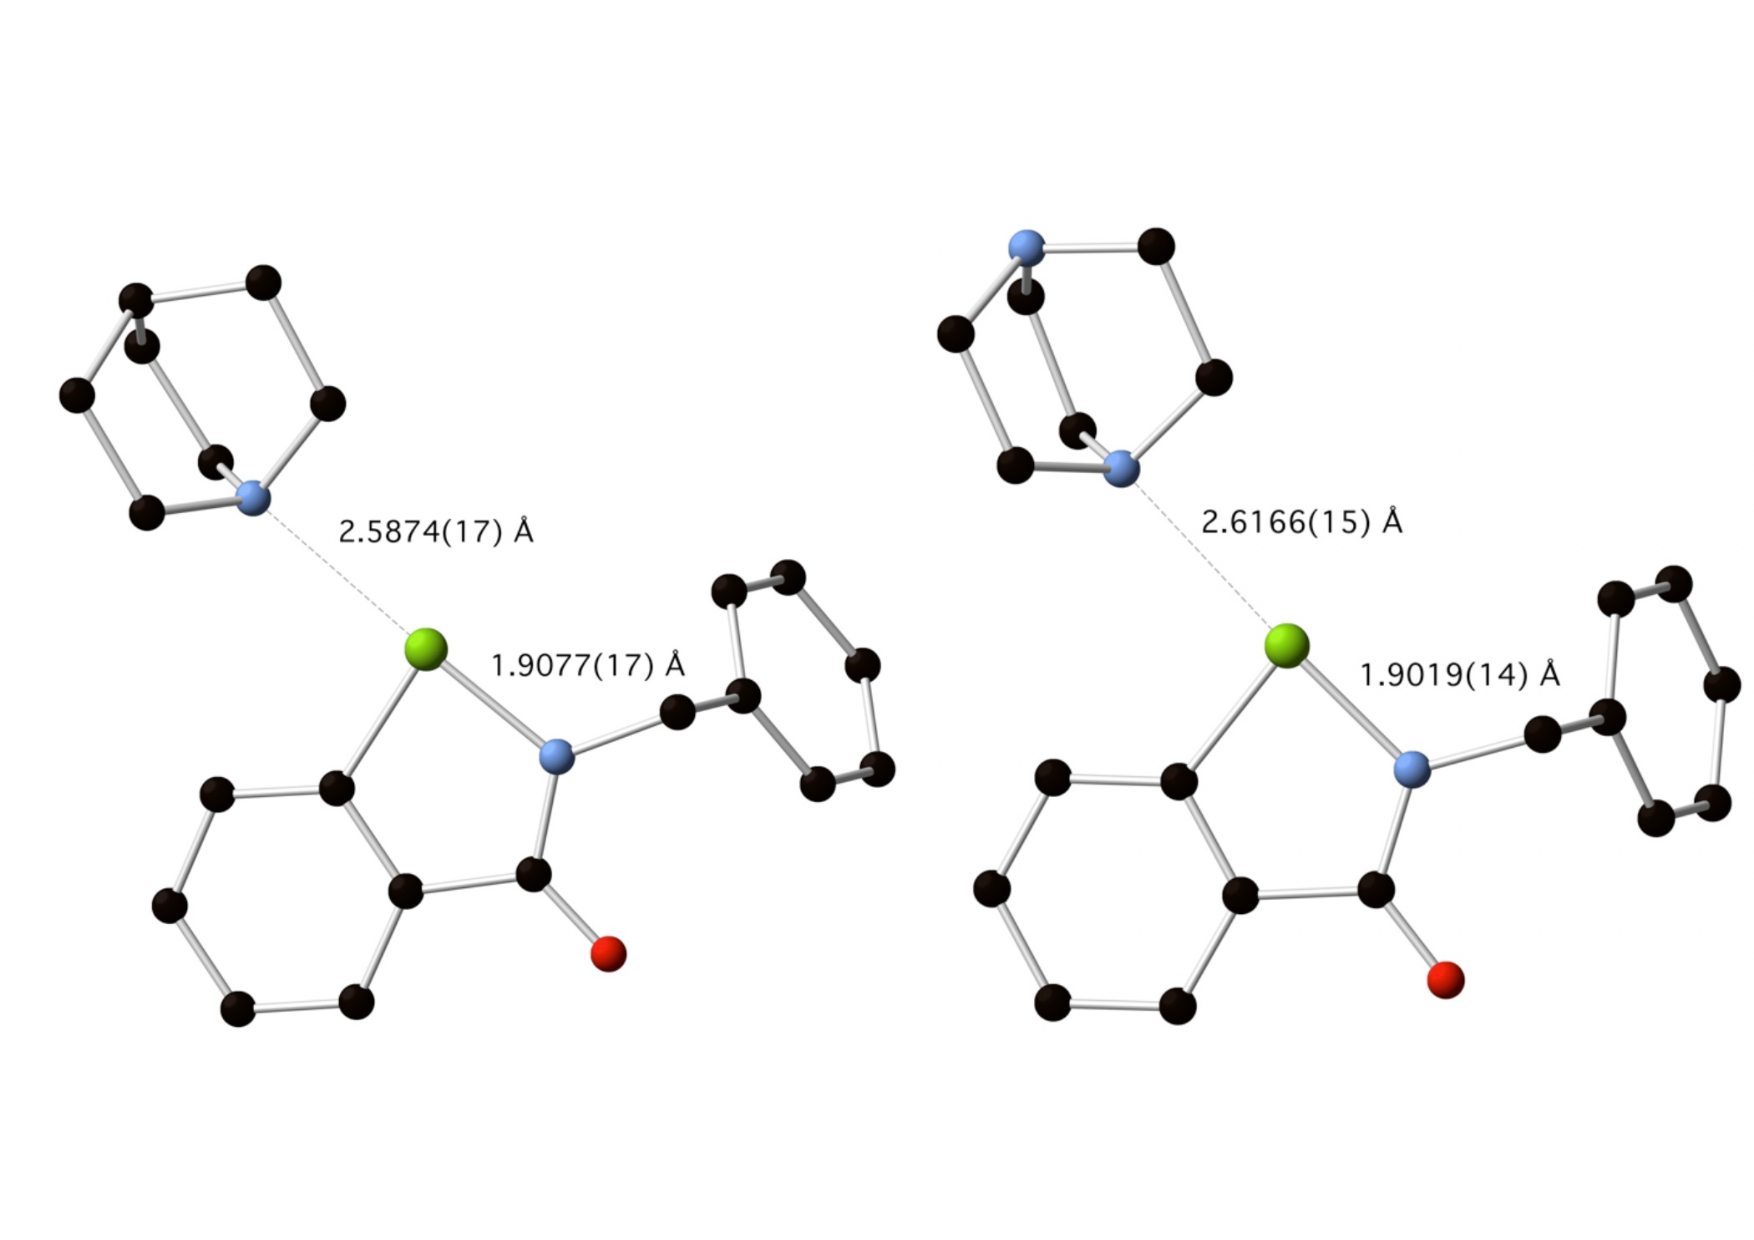
\includegraphics[width=0.8\linewidth]{Figures/benzyl-quin-dabco-xray.pdf}
  \caption{Adducts of benzisoselenazolinone \refcmpd{ebs.bn} with quinuclidine and DABCO.}
  \label{fig:benzyl-adducts}
\end{figure}

\subsection{DFT interaction energies, NBO and NEDA analysis}
Interaction energies for the complexes were calculated using the $\omega$B97X-D dispersion corrected functional, which has been used to study similar systems with good agreement with coupled cluster methods.\autocite{Oliveira2017}
All geometries were therefore optimized at $\omega$B97X-D/def2TZVP, and minima verified by frequency analysis.

\begin{figure}
  \centering
  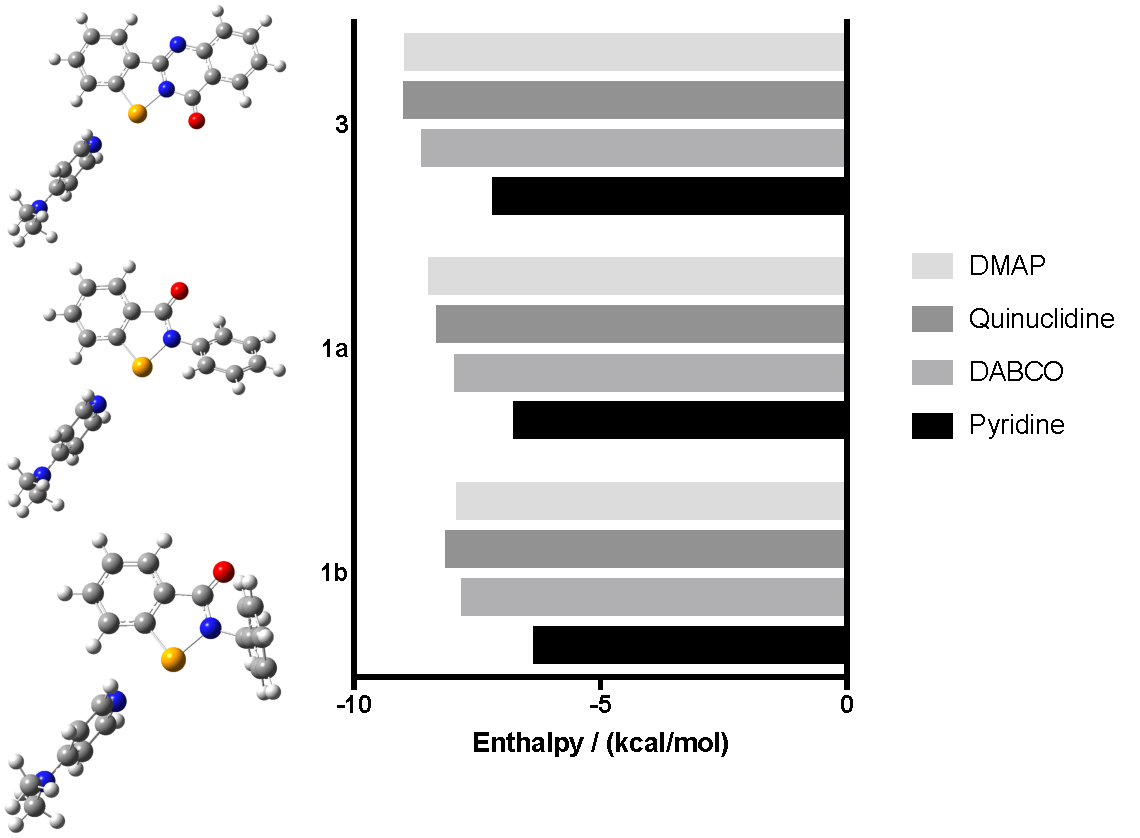
\includegraphics[width=0.8\linewidth]{Figures/dft-energies.pdf}
  \caption[Interaction energies for various complexes.]{Interaction enthalpies calculated at $\omega$B97X-D/def2TZVP. Optimised geometries for the DMAP complexes are shown to the left.}
\end{figure}

NBO analysis was conducted on the optimized geometries, which supports our suggestion that there is a strong orbital component to Ch-bonding in these systems.
Second order perturbation theory revealed that the energy associated with n(N\textsubscript{base})$\rightarrow$ $\sigma^{\star}$(N\textsubscript{1}--Se) delocalization was 12.79, 15.45, and 16.23~kcal/mol for \cmpd{ebs.bn}$\cdot$DMAP, \cmpd{ebs.ph}$\cdot$DMAP, and \cmpd{tetracycle}$\cdot$DMAP respectively.
%In the case of the \cmpd{ebs.bn}$\cdot$DMAP$\cdot$\ce{H2O} complex, the delocalization energy was 13.51~kcal/mol.
%This consistent with our experimental observation of hydrogen-bond enhanced Ch-bonding.

\begin{figure}
  \centering
  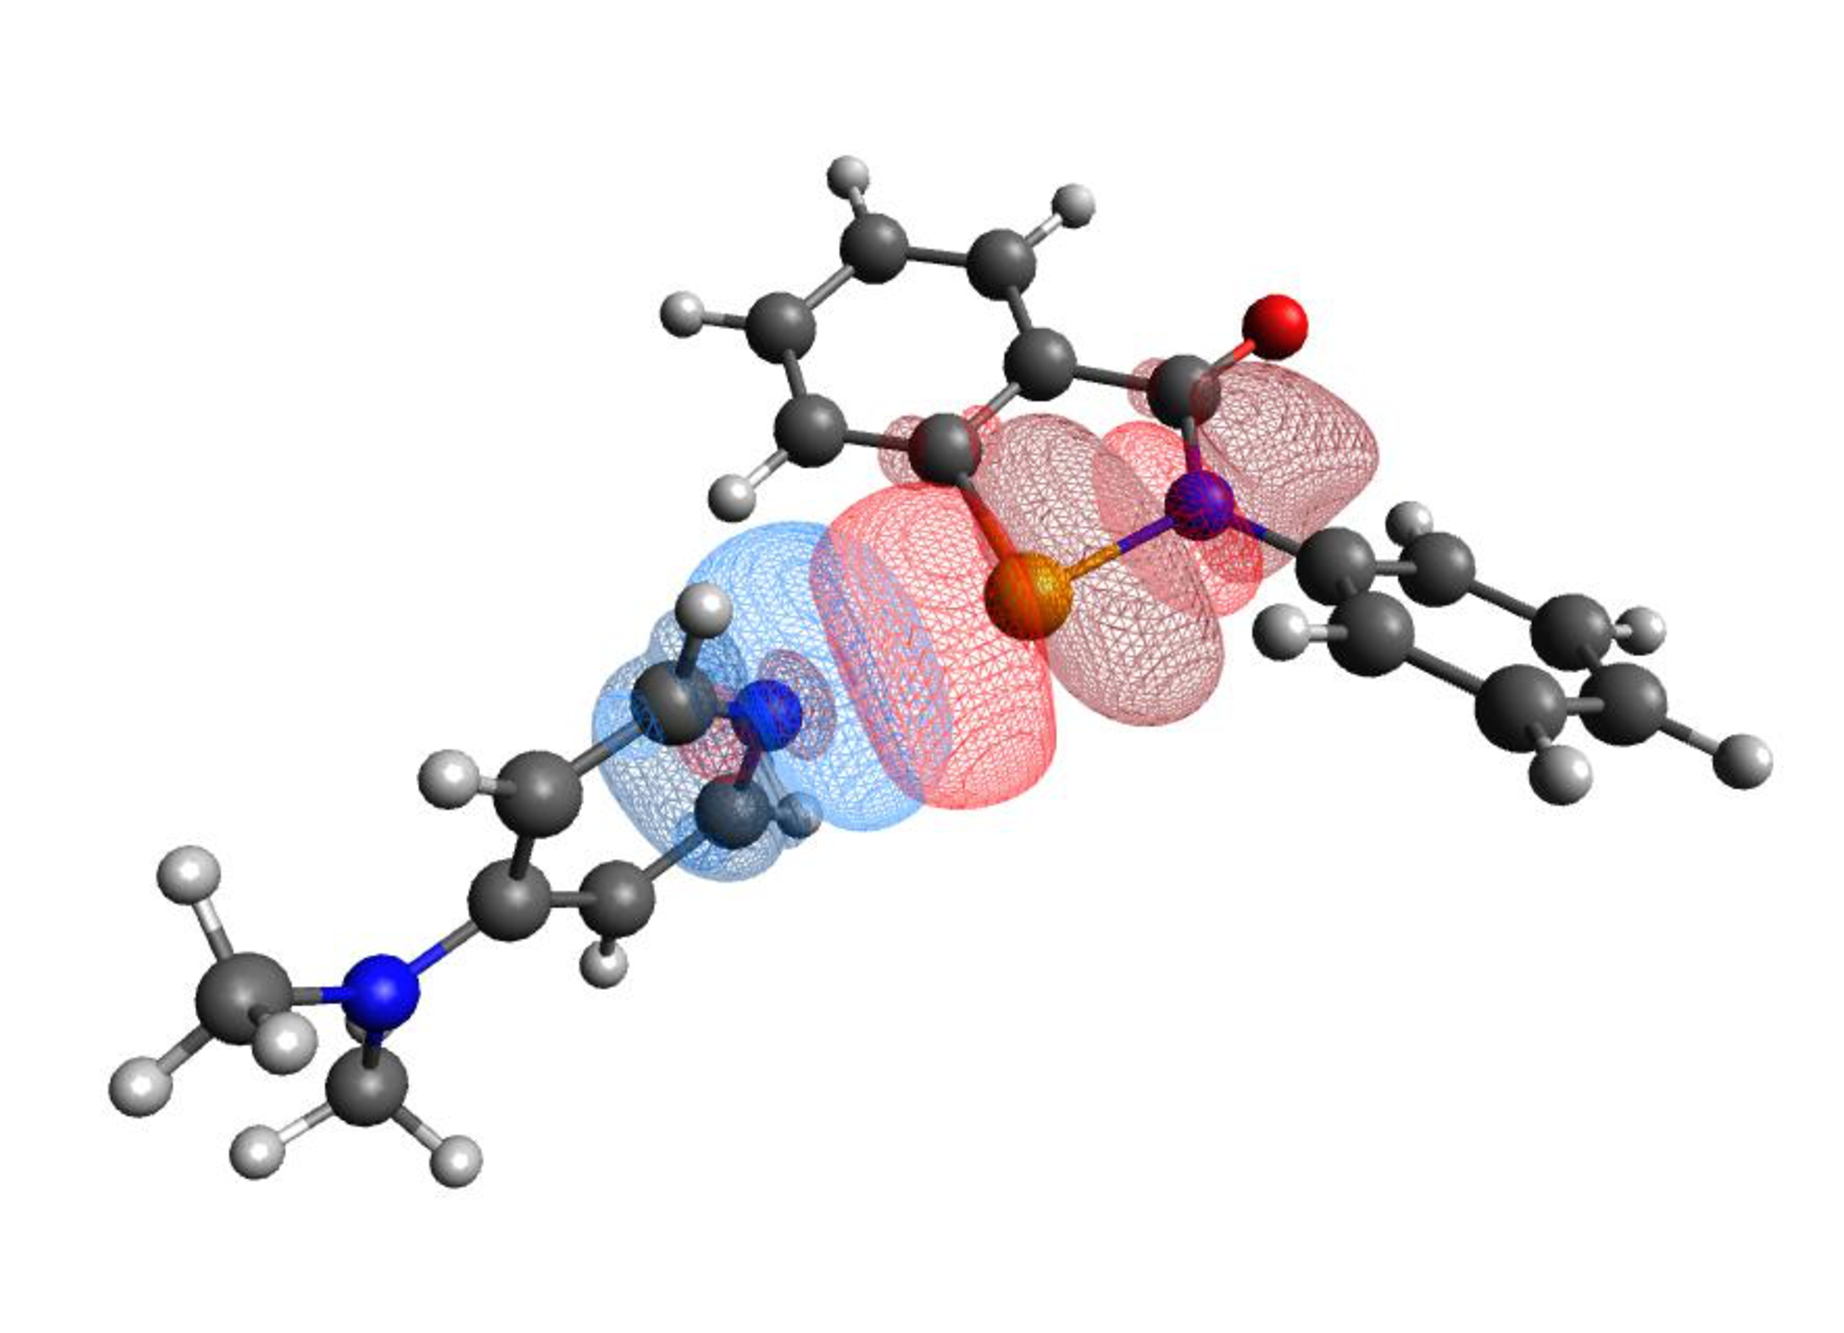
\includegraphics[width=0.6\linewidth]{Figures/phenyl-dmap-overlap.pdf}
  \caption[Orbital overlap for \refcmpd{ebs.ph}$\cdot$DMAP.]{Overlap of nitrogen lone pair with $\sigma^{\star}$(Se - N) in \refcmpd{ebs.ph}$\cdot$DMAP complex.}
  \label{fig:phenyl-dmap-overlap}
\end{figure}

\section{Conclusion}
In summary, we have demonstrated the importance of Ch-bonding between derivatives of ebselen \cmpd{ebs.ph} and a variety of nitrogen bases.
These selenium-containing heterocycles form close contacts with electron pair donors, well within the Van der Waals radii, with predictable geometries consistent with the Ch-bonding model.
These interactions appear to be primarily due to orbital overlap as opposed to electrostatic or dispersion mediated effects, as evidenced by lengthening of the antipodal Se--N bond, and computational analysis, which is consistent with findings in related systems by Cockroft \emph{et al}.\autocite{Pascoe2017}
We have also found that the strength of a Ch-bond can be enhanced \emph{via} a hydrogen bond to the carbonyl group of the heterocycle.
We hope to exploit the strength and directionality of Ch-bonds in ebselen to target biomolecules such as nucleic acids and proteins using compounds containing the isoselenazolone moiety.

\section{Supplementary materials}

\subsection{Synthetic procedures}

\subsubsection[Preparation of \refcmpd{ebs.ph}.]{Preparation of 2-phenylbenzo[\emph{d}][1,2]selenazol-3(2\emph{H})-one \refcmpd{ebs.ph}.}

Copper iodide (98.4~mg, 0.517~mmol) and 1,10-phenanthroline (83.1~mg, 0.461~mmol) were stirred in anhydrous DMF (3~mL) for 15 mins at r.t., then 2-iodo-N-phenylbenz\-amide (653.2~mg, 2.021~mmol), selenium (196.9~mg, 2.495~mmol) and potassium carbonate (627.3~mg, 4.539~mmol) were added sequentially under a flow of argon. 
The mixture was heated at 110\degree C for 8~h, when TLC showed consumption of starting material. 
The mixture was then tipped into brine (30~mL) and stirred to form a brown precipitate, which was extracted into DCM (40~mL) and washed with water (2 $\times$ 20~mL). 
The DCM solution was filtered through a silica plug, then evaporated, and the residue applied to a SNAP 25~g silica cartridge, eluting with a petroleum ether/ethyl acetate gradient. 
The major peak was evaporated to afford colourless crystals of \cmpd{ebs.ph} (378.8~mg, 69\%, m.p. 179.1--180.3\degree C, lit. mp 180--181\degree C). \textsuperscript{77}Se NMR $\delta$ 959.66.

\subsubsection[Preparation of \refcmpd{ebs.bn}.]{Preparation of 2-benzylbenzo[\emph{d}][1,2]selenazol-3(2\emph{H})-one \refcmpd{ebs.bn}.}

Copper iodide (95.8~mg, 0.503~mmol) and 1,10-phenanthroline (93.8~mg, 0.521~mmol) were stirred in anhydrous DMF (3~mL) for 15 mins at r.t., then N-benzyl-2-iodobenzamide (860.9~mg, 2.553~mmol), selenium (256.6~mg, 3.249~mmol) and potassium carbonate (542.2~mg, 3.923~mmol) were added sequentially under a flow of argon. 
The mixture was heated at 110\degree C for 5~h, when TLC showed consumption of starting material. 
The mixture was then tipped into brine (30~mL) and stirred to form a solid mass, which was dissolved in DCM (40~mL) and washed with water (2 $\times$ 20~mL). 
The DCM solution was filtered through a silica plug, then evaporated, and the residue applied to a SNAP 50~g silica cartridge, eluting with a petroleum ether/ethyl acetate gradient. 
The major peak was evaporated to afford pale yellow crystals of \cmpd{ebs.bn} (396.4~mg, 53\%, m.p. 137.8--138.8\degree C). \textsuperscript{77}Se NMR $\delta$ 884.02.

\subsubsection[Preparation of \refcmpd{tetracycle}.]{Preparation of 5\emph{H}-benzo[4,5][1,2]selenazolo[2,3-\emph{a}]quinazolin-5-one \refcmpd{tetracycle}.}

Copper iodide (96.4~mg, 0.503~mmol) and 1,10-phenanthroline (85.7~mg, 0.476~mmol) were stirred in anhydrous DMF (4~mL) for 10~mins at r.t., then 2-iodobenzamide (510.6~mg, 2.067~mmol), selenium (209.5~mg, 2.653~mmol) and potassium carbonate (506.3~mg, 3.663~mmol) were added sequentially under a flow of argon. 
The mixture was heated at 110\degree C for 12~h, when TLC showed consumption of starting material. 
The mixture was then tipped into brine (30~mL) and stirred to form a solid mass, which was extracted into ethyl acetate (20~mL) and washed with water (2 $\times$ 20~mL).
The DCM solution was filtered through a silica plug, then evaporated, and the residue applied to a SNAP 50~g silica cartridge, eluting with a petroleum ether/ethyl acetate gradient. 
The major peak was evaporated to afford pale yellow crystals of \cmpd{tetracycle} (45.8~mg, 15\%, m.p. 267--268\degree C). \textsuperscript{77}Se NMR $\delta$ 992.48.

\subsection{Crystallographic data}
Intensity data was collected on an Oxford Diffraction SuperNova CCD diffractometer using either Cu-K$\alpha$ or Mo-K$\alpha$ radiation at 130.0(1)~K, or on a Rigaku XtalLAB Synergy at 100.0(1)~K. Compound \cmpd{ebs.bn}$\cdot$DMAP$\cdot$\ce{H2O} underwent a destructive phase change when cooling to 130~K, therefore data were collected at 200~K. Data for \cmpd{tetracycle} was collected on the MX1 beamline at the Australian Synchrotron\autocite{Cowieson2015}. The temperature was maintained using an Oxford Cryostream cooling device. The structures were solved by direct methods and difference Fourier synthesis.\autocite{Sheldrick2015} Thermal ellipsoid plot was generated using the program ORTEP-3\autocite{Farrugia1997} integrated within the WINGX\autocite{Farrugia1999} suite of programs.  

\subsubsection{Crystal data for \texorpdfstring{\refcmpd{ebs.ph}$\cdot$DMAP}{C20H19N3OSe}}
\ce{C20H19N3OSe}, $M=396.34$, $T=130.0$~K, $\lambda=0.71073$~\AA, Triclinic, space group P$\bar{1}$, $a = 8.3674(3)$, $b = 9.8399(5)$, $c =10.6622(5)$~\AA, $\alpha=93.296(4)$\degree, $\beta=93.021(4)$\degree, $\gamma=101.210(4)$\degree, $V=857.86(7)$~\AA$^{3}$, $Z = 2$.
$D_{c}= 1.534$~mg~M$^{-3}$, $\mu$(Mo-K$\alpha$) = 2.201~mm$^{-1}$, F(000) = 404, crystal size $0.52 \times 0.34 \times 0.23$~mm.
11339 reflections measured, $\theta_{\mathrm{max}}=36.66$\degree, 7889 independent reflections, R\textsubscript{int} = 0.0163, the final R was 0.0293 ($I > 2\theta(I)$, 6882 reflections) and \emph{w}R(F\textsuperscript{2}) was 0.0721 (all data), GOF 0.992. 
CCDC 1867205. 
From dichloromethane/pentane (70\%) m.p. 111.3--112.1\degree C.

\subsubsection{Crystal data for \texorpdfstring{\refcmpd{ebs.bn}}{C14H11NOSe}}
\ce{C14H11NOSe}, $M=288.20$, $T=100.0$~K, $\lambda=0.71073$~\AA, Orthorhombic, space group Pca2\textsubscript{1}, $a = 11.7848(3)$, $b = 4.5869(1)$, $c = 21.3572(5)$~\AA, $V = 1154.48(5)$~\AA$^{3}$, $Z = 4$.
$D_{c}= 1.658$~mg~M$^{-3}$, $\mu$(Mo-K$\alpha$) = 3.233~mm$^{-1}$, F(000) = 576, crystal size $0.63 \times 0.54 \times 0.22$~mm.
44918 reflections measured, $\theta_{\mathrm{max}}=45.38$\degree, 9588 independent reflections, R\textsubscript{int} = 0.0481, the final R was 0.0331 ($I > 2\theta(I)$, 7848 reflections) and \emph{w}R(F\textsuperscript{2}) was 0.0792 (all data), GOF 1.063. 
CCDC 1867211. 

\subsubsection{Crystal data for \texorpdfstring{\refcmpd{ebs.bn}$\cdot$DMAP$\cdot$\ce{H2O}}{C21H21N3OSe.(H2O)}}
\ce{C21H21N3OSe.(H2O)}, $M=428.38$, $T=200.0$~K, $\lambda=0.71073$~\AA, Triclinic, space group P$\bar{1}$, $a = 9.6254(2)$, $b = 10.2486(2)$, $c = 10.6505(2)$~\AA, $\alpha = 83.660(2)$\degree, $\beta = 76.398(2)$\degree, $\gamma = 78.423(2)$\degree, $V = 998.19(4)$~\AA$^{3}$, $Z = 2$.
$D_{c}= 125$~mg~M$^{-3}$, $\mu$(Mo-K$\alpha$) = 1.901~mm$^{-1}$, F(000) = 440, crystal size $0.41 \times 0.32 \times 0.23$~mm.
30047 reflections measured, $\theta_{\mathrm{max}} = 41.06$\degree, 12528 independent reflections, R\textsubscript{int} = 0.0267, the final R was 0.0456 ($I > 2\theta(I)$, 6303 reflections) and \emph{w}R(F\textsuperscript{2}) was 0.1219 (all data), GOF 1.000. 
CCDC 1867213. 
From THF in an open flask (90\%) m.p. 96--97\degree C.

\subsubsection{Crystal data for \texorpdfstring{\refcmpd{ebs.bn}$\cdot$DMAP}{C21H21N3OSe}}
\ce{C21H21N3OSe}, $M=410.37$, $T=130.0$~K, $\lambda=0.71073$~\AA, Triclinic, space group P$\bar{1}$, $a = 9.6002(4)$, $b = 10.2109(4)$, $c = 19.8380(7)$~\AA, $\alpha = 78.710(3)$\degree, $\beta = 84.901(3)$\degree, $\gamma = 77.458(4)$\degree, $V = 1859.33(13)$~\AA$^{3}$, $Z = 4$, $Z\prime = 2$.
$D_{c}= 1.466$~mg~M$^{-3}$, $\mu$(Mo-K$\alpha$) = 2.034~mm$^{-1}$, F(000) = 840, crystal size $0.65 \times 0.24 \times 0.37$~mm.
36541 reflections measured, $\theta_{\mathrm{max}} = 40.95$\degree, 23437 independent reflections, R\textsubscript{int} = 0.0264, the final R was 0.0448 ($I > 2\theta(I)$, 15177 reflections) and \emph{w}R(F\textsuperscript{2}) was 0.1120 (all data), GOF 1.044. 
CCDC 1867209. 
From dichloromethane/pentane (60\%) m.p. 86.1--92.5\degree C.

\subsubsection{Crystal data for \texorpdfstring{\refcmpd{ebs.bn}$\cdot$quinuclidine}{C21H24N2OSe}}
\ce{C21H24N2OSe}, $M=399.38$, $T=130.0$~K, $\lambda=1.54184$~\AA, Monoclinic, space group P2\textsubscript{1}/c, $a = 10.1610(2)$, $b = 16.0506(3)$, $c = 11.4300(2)$~\AA, $\beta = 104.622(2)$\degree, $V = 1803.75(6)$~\AA$^{3}$, $Z = 4$.
$D_{c}= 1.471$~mg~M$^{-3}$, $\mu$(Cu-K$\alpha$) = 3.895~mm$^{-1}$, F(000) = 824, crystal size $0.29 \times 0.10 \times 0.03$~mm.
12588 reflections measured, $\theta_{\mathrm{max}} = 77.19$\degree, 3771 independent reflections, R\textsubscript{int} = 0.0379, the final R was 0.0329 ($I > 2\theta(I)$, 3397 reflections) and \emph{w}R(F\textsuperscript{2}) was 0.0849 (all data), GOF 1.028. 
CCDC 1867207. 
From dichloromethane/pentane (50\%) m.p. 135.2--137.4\degree C.

\subsubsection{Crystal data for \texorpdfstring{\refcmpd{ebs.bn}$\cdot$DABCO}{C20H23N3OSe}}
\ce{C20H23N3OSe}, $M=400.37$, $T=130.0$~K, $\lambda=1.54184$~\AA, Monoclinic, space group P2\textsubscript{1}/c, $a = 10.1249(2)$, $b = 15.9246(3)$, $c = 11.4660(2)$~\AA, $\beta = 106.572(2)$\degree, $V = 1771.93(6)$~\AA$^{3}$, $Z = 4$.
$D_{c} = 1.501$~mg~M$^{-3}$, $\mu$(Cu-K$\alpha$) = 2.965~mm$^{-1}$, F(000) = 824, crystal size $0.37 \times 0.17 \times 0.04$~mm.
13121 reflections measured, $\theta_{\mathrm{max}} = 77.12$\degree, 3711 independent reflections, R\textsubscript{int} = 0.0280, the final R was 0.0258 ($I > 2\theta(I)$, 3333 reflections) and \emph{w}R(F\textsuperscript{2}) was 0.0657 (all data), GOF 1.056. 
CCDC 1867206. 
From dichloromethane/pentane (65\%) m.p. 131.4--133.3\degree C.

\subsubsection{Crystal data for \texorpdfstring{\refcmpd{tetracycle}}{C14H8N2OSe}}
\ce{C14H8N2OSe}, $M=299.18$, $T=100.0$~K, $\lambda=0.71092$~\AA, Orthorhombic, space group Pca2\textsubscript{1}, $a = 17.371(4)$, $b = 5.3080(11)$, $c = 11.633(2)$~\AA, $V = 1072.6(4)$~\AA$^{3}$, $Z = 4$.
$D_{c}= 1.853$~mg~M$^{-3}$, $\mu$(Mo-K$\alpha$) = 3.486~mm$^{-1}$, F(000) = 592, crystal size $0.15 \times 0.10 \times 0.02$~mm.
16031 reflections measured, $\theta_{\mathrm{max}}=31.56$\degree, 2967 independent reflections, R\textsubscript{int} = 0.0363, the final R was 0.0271 ($I > 2\theta(I)$, 2061 reflections) and \emph{w}R(F\textsuperscript{2}) was 0.0751 (all data), GOF 1.129. 
CCDC 1867208. 

\subsubsection{Crystal data for \texorpdfstring{\refcmpd{tetracycle}$\cdot$pyridine}{C19H13N3OSe}}
\ce{C19H13N3OSe}, $M=378.28$, $T=130.0$~K, $\lambda=1.54184$~\AA, Monoclinic, space group P2\textsubscript{1}/c, $a = 20.7476(9)$, $b = 4.9407(2)$, $c = 17.6687(7)$~\AA, $\beta = 107.376(4)$\degree, $V = 1156.27(5)$~\AA$^{3}$, $Z = 4$.
$D_{c} = 1.454$~mg~M$^{-3}$, $\mu$(Cu-K$\alpha$) = 3.018~mm$^{-1}$, F(000) = 760, crystal size $0.56 \times 0.05 \times 0.03$~mm.
5766 reflections measured, $\theta_{\mathrm{max}} = 75.76$\degree, 3419 independent reflections, R\textsubscript{int} = 0.0301, the final R was 0.0346 ($I > 2\theta(I)$, 2889 reflections) and \emph{w}R(F\textsuperscript{2}) was 0.0955 (all data), GOF 1.054. 
CCDC 1867211. 
From dichloromethane/pentane (70\%) m.p. 247.5--248.4\degree C.

\subsubsection{Crystal data for \texorpdfstring{\refcmpd{tetracycle}$\cdot$DMAP}{C21H18N4OSe}}
\ce{C21H18N4OSe}, $M = 421.35$, $T=100.0$~K, $\lambda=0.71073$~\AA, Triclinic, space group P$\bar{1}$, $a = 8.8093(2)$, $b = 10.7445(2)$, $c = 10.9812(2)$~\AA, $\alpha = 111.687(2)$\degree, $\beta = 109.283(2)$\degree, $\gamma = 96.631(2)$\degree, $V = 877.57(3)$~\AA$^{3}$, $Z = 2$, $Z\prime = 2$.
$D_{c}= 1.595$~mg~M$^{-3}$, $\mu$(Mo-K$\alpha$) = 2.159~mm$^{-1}$, F(000) = 428, crystal size $0.18 \times 0.11 \times 0.06$~mm.
56053 reflections measured, $\theta_{\mathrm{max}} = 41.07$\degree, 11273 independent reflections, R\textsubscript{int} = 0.0547, the final R was 0.0358 ($I > 2\theta(I)$, 8667 reflections) and \emph{w}R(F\textsuperscript{2}) was 0.0872 (all data), GOF 1.048. 
CCDC 1867212. 
From dichloromethane/pentane (80\%) m.p. 248.8--249.4\degree C.

\printbibliography[heading=subbibliography]
\end{refsection}


\begin{refsection}

\chapter{Further investigations into Ch-bonded complexes}

\section{Introduction}
In the previous chapter, we established that Ch-bonding is not only present in ebselen derivatives, but dominates packing in crystals of the pure compound (through \ce{Se\cdots O} interactions) and in co-crystals with a variety of Lewis bases.
In this chapter, we extend our investigation to a wider range of derivatives with systematically varied electronic properties.

Linear free energy relationships are...

\section{Results and discussion}
Our previous work had shown that electron-rich pyridines (specifically DMAP) formed the strongest Ch-bonds out of all the bases trialled. 
This is roughly consistent with the hydrogen bond basicity (pK\textsubscript{HB}) of the bases (\cref{tab:pkhb}).
Methyl cation affinities?\autocite{Wei2008MethylOrganocatalysts}
The planar geometry and aromatic character of DMAP may also facilitate crystallisation, as opposed to the relatively bulky and flexible aliphatic bases which may not pack as efficiently.
For these reasons, we restricted the bases used in this study to other electron-rich pyridines.
Although DMAP is already a very strong base, the basisicity can be increased by incorporating the aniline nitrogen in another ring.
This reduces the energetic penalty associated with the delocalisation of the lone pair into the pyridine ring, by forcing a more planar geometry upon the nitrogen.\autocite{Berthelot1998,Heinrich2003EnhancingFixation}
Compounds \cmpd{py.pyrrol,py.morph} were therefore synthesised by treating 4-chloropyridine hydrochloride with 2 equivalents of the appropriate base (\cref{sch:base-synthesis}).

\begin{scheme}
\centering
\replacecmpd[sub-only]{py.pyrrol}
\replacecmpd[sub-only]{py.morph}
\replacecmpd{py.{pyrrol,morph}}
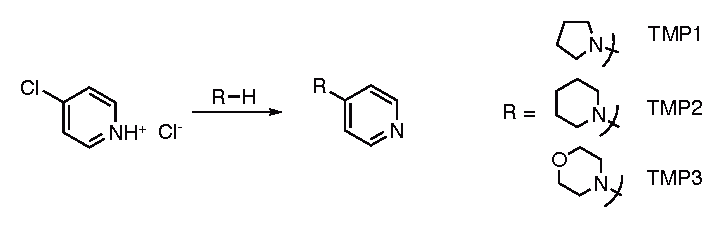
\includegraphics[scale=0.8]{Figures/base-synthesis.eps}
\caption{Synthesis of Lewis bases \refcmpd{py.pyrrol,py.morph}.}
\label{sch:base-synthesis}
\end{scheme}

The benzisoselenazolone derivatives \cmpd{ebs.{ph,4no2,4cn,4cf3,4br,4co2et,4me,4ome,4oet}} were prepared by the reaction of substituted anilines with a selenenyl chloride intermediate \cmpd{diselenide}, ultimately derived from anthranilic acid (\cref{sch:ebs-synthesis}).
The one-pot selenocyclisation reaction used in the previous work often did not tolerate the various functional groups on the aryl ring, affording reduction, cross-coupling, or protodehalogenation byproducts. 
All derivatives except \cmpd{ebs.4no2} were isolated in acceptable yield at room temperature, using acetonitrile as a solvent, and in the presence of a weak base (triethylamine).
Due to the strongly electron-withdrawing nature of the nitro substituent, the parent aniline of \cmpd{ebs.4no2} was not sufficiently nucleophilic to react under the same conditions.
We therefore first deprotonated the aniline using \ce{NaH} (60\% suspension in mineral oil) in anhydrous THF before adding the selenyl chloride, which afforded the benzisoselenazolone in excellent yield.

We also note the solubility trends of the products as the electron demand of the substituent increases.
The electron rich derivatives \cmpd{ebs.4ome,ebs.4oet,ebs.4me} were highly soluble even in relatively poor solvents (\ce{Et2O}, \ce{EtOAc}), while the electron poor derivatives \cmpd{ebs.4no2,ebs.4cn} were insoluble in all but the strongest solvents (DMSO).
This likely reflects the varying strength of the crystal packing due to the \ce{Se\cdots O=C} Ch-bond.

\begin{scheme}
\centering
\replacecmpd{diselenide}
\replacecmpd{ebs.{ph,4no2,4cn,4cf3,4br,4co2et,4me,4ome,4oet}}
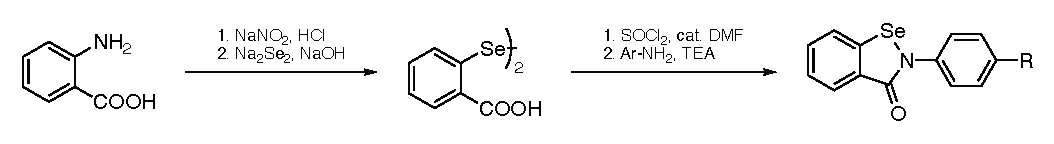
\includegraphics[scale=0.8]{Figures/ebs-synthesis.eps}

\vspace{0.6cm}

\footnotesize{
\begin{tabular}{cccccc}\toprule
    Compound & R = & Compound & R = & Compound & R = \\\midrule
    \cmpd{ebs.ph} & \ce{-H} & \cmpd{ebs.4cf3} & \ce{-CF3} & \cmpd{ebs.4me} & \ce{-CH3}\\
    \cmpd{ebs.4no2} & \ce{-NO2} & \cmpd{ebs.4br} & \ce{-Br} & \cmpd{ebs.4ome} & \ce{-OMe}\\
    \cmpd{ebs.4cn} & \ce{-CN} & \cmpd{ebs.4co2et} & \ce{-CO2Et} & \cmpd{ebs.4oet} & \ce{-OEt} \\\bottomrule
\end{tabular}}
\caption{Synthesis of benzisoselenazolone derivatives \refcmpd{ebs.{ph,4no2,4cn,4cf3,4br,4co2et,4me,4ome,4oet}}.}

\label{sch:ebs-synthesis}
\end{scheme}

Co-crystals of the benzisoselenazolones and pyridines were grown by vapour diffusion from an equimolar solution in dichloromethane/pentane. 
Relevant structural parameters are given in \cref{tab:bondlengths2}.
In addition to the structural parameters, we characterised the various Ch-bonds using Bader's QTAIM framework.
Depending on the quality of the data we were able to obtain for each crystal, we used:

\begin{itemize}
    \item experimental electron density from a multipole refinement with atomic coordinates determined from high angle refinement ($d < 0.8$\AA), 
    \item experimental electron density from a multipole refinement with atomic coordinates determined by refinement using aspherical scattering factors derived from the DFT electron density,
    \item density derived from the DFT calculation.
\end{itemize}

The second ``hybrid'' strategy has the advantage of being able to capture electron density effects not fully described by DFT, while not requiring a large amount of weak high-angle (or neutron) data for the reliable determination of atomic coordinates.
The low-angle data, however, does need to be free from faults, so this strategy may still not be appropriate for all data sets.

\begin{table}
  \centering
  \caption{Selected structural and electron density parameters of Ch-bonded complexes.}
  \small
  \tablefit{\begin{tabular}{lllllllll}
    \toprule
    Complex & r(N$\cdots$Se) & r(Se--N\textsubscript{1}) & r(Se--C\textsubscript{1}) & r(N\textsubscript{1}--C(O)) & $\angle$(N$\cdots$Se--N\textsubscript{1}) & $\angle$(C\textsubscript{para}$\cdots$N$\cdots$Se) & $\rho_{\mathrm{BCP}}$(\ce{Se\cdots N}) & $\nabla^{2}(\rho_{\mathrm{BCP})}$(\ce{Se\cdots N}) \\
      & \AA\ & \AA\ & \AA\ & \AA\ & $^\circ$ & $^\circ$ & e/\AA$^3$ & e/\AA$^5$ \\ \midrule
    \cmpd{ebs.ph}                       & --- & 1.896(3) & 1.892(4) & 1.359(5) & --- & --- & --- & --- \\
    \cmpd{ebs.4no2}                     & --- \\
    \cmpd{ebs.4cn}                      & --- & 1.894(2) & 1.877(2) & 1.372(2) & --- & --- & --- & --- \\
    \cmpd{ebs.4cf3}\footnote{\label{fn:enva}Environment \textit{a}} & --- & 1.880(9) & 1.889(9) & 1.38(1) & --- & --- & --- & --- \\
    \cmpd{ebs.4cf3}\footnote{\label{fn:envb}Environment \textit{b}} & --- & 1.898(8) & 1.901(9) & 1.37(1) & --- & --- & --- & --- \\
    \cmpd{ebs.4br}                      & --- & 1.898(2) & 1.889(2) & 1.371(3) & --- & --- & --- & --- \\
    \cmpd{ebs.4co2et}                   & --- & 1.902(2) & 1.879(2) & 1.371(3) & --- & --- & --- & --- \\
    \cmpd{ebs.4me}                      & --- & 1.904(3) & 1.890(3) & 1.365(4) & --- & --- & --- & --- \\
    \cmpd{ebs.4ome}                     & --- & 1.8741(9) & 1.887(1) & 1.356(1) & --- & --- & --- & --- \\
    \cmpd{ebs.4oet}                     & --- & 1.901(3) & 1.885(4) & 1.357(4) & --- & --- & --- & --- \\\\
    
    \cmpd{ebs.ph}$\cdot$DMAP     & 2.371(1) & 1.968(1) & 1.896(1) & 1.358(2) & 174.18(4) & 173.51(6) & 0.3511 & 2.6960 \footnote{\label{fn:fullmultipole}Fully experimental density used} \\
    \cmpd{ebs.4no2}$\cdot$DMAP   & 2.2424(5) & 2.0200(4) & 1.9086(4) & 1.3592(4) & 173.57(2) & 175.47(2) & 0.5372 & 3.8680 \textsuperscript{\ref{fn:fullmultipole}} \\
    \cmpd{ebs.4cn}$\cdot$DMAP    & 2.301(1) & 1.997(1) & 1.899(2) & 1.368(2) & 174.79(5) & 167.57(6) & 0.4130 & 2.5210 \textsuperscript{\ref{fn:fullmultipole}} \\
    \cmpd{ebs.4cn}$\cdot$DMAP\footnote{\label{fn:solvate}DCM solvate}\textsuperscript{,\ref{fn:enva}}  & 2.254(2) & 2.019(2) & 1.902(1) & 1.366(2) & 174.46(6) & 176.33(7) & 0.4780 & 2.4816 \footnote{\label{fn:dftdens}DFT density used} \\
    \cmpd{ebs.4cn}$\cdot$DMAP\textsuperscript{\ref{fn:solvate},\ref{fn:envb}}  & 2.308(2) & 1.993(1) & 1.901(1) & 1.372(2) & 174.93(5) & 167.85(7) & 0.4284 & 2.4558 \textsuperscript{\ref{fn:dftdens}} \\
    \cmpd{ebs.4cf3}$\cdot$DMAP   & 2.3347(9) & 1.9855(9) & 1.899(1) & 1.372(1) & 175.24(4) & 162.65(5) & 0.4048 & 2.4112 \textsuperscript{\ref{fn:dftdens}}\\
    \cmpd{ebs.4br}$\cdot$DMAP    & 2.3215(7) & 1.9840(7) & 1.9021(8) & 1.362(1) & 173.85(3) & 173.56(4) & 0.4058 & 3.1160 \\
    \cmpd{ebs.4co2et}$\cdot$DMAP\textsuperscript{\ref{fn:solvate}} & 2.322(1) & 1.982(1) & 1.902(1) & 1.367(2) & 174.96(4) & 172.86(6) \\
    \cmpd{ebs.4me}$\cdot$DMAP    & 2.4301(4) & 1.9341(4) & 1.8918(4) & 1.3650(6) & 175.33(1) & 158.64(2) \\
    \cmpd{ebs.4ome}$\cdot$DMAP\footnote{\label{fn:p1}Polymorph 1}\textsuperscript{,\ref{fn:enva}}  & 2.270(1) & 1.9689(9) & 1.899(1) & 1.350(1) & 174.17(3) & 159.44(4) \\
    \cmpd{ebs.4ome}$\cdot$DMAP\textsuperscript{\ref{fn:p1},\ref{fn:envb}}  & 2.4496(9) & 1.9267(9) & 1.895(1) & 1.357(1) & 174.57(3) & 160.53(4) \\
    \cmpd{ebs.4ome}$\cdot$DMAP\footnote{\label{fn:p2}Polymorph 2}\textsuperscript{,\ref{fn:enva}}  & 2.334(1) & 1.965(1) & 1.894(1) & 1.363(1) & 175.95(5) & 155.71(6) \\
    \cmpd{ebs.4ome}$\cdot$DMAP\textsuperscript{\ref{fn:p2},\ref{fn:envb}}  & 2.407(1) & 1.941(1) & 1.894(1) & 1.358(2) & 176.12(5) & 156.60(6) \\
    \cmpd{ebs.4oet}$\cdot$DMAP\textsuperscript{\ref{fn:enva}}   & 2.517(2) & 1.921(1) & 1.895(2) & 1.356(3) & 172.30(6) & 158.37(8) \\
    \cmpd{ebs.4oet}$\cdot$DMAP\textsuperscript{\ref{fn:envb}}   & 2.327(5) & 1.931(2) & 1.894(2) & 1.353(3) & 171.4(1) & 151.2(3) \\\\
    
    \cmpd{ebs.ph}$\cdot$\cmpd{py.pyrrol}     & 2.350(1) & 1.9830(9) & 1.8985(7) & 1.3616(8) & 174.20(3) & 176.46(4) & 0.2419 & 5.4650 \\
    \cmpd{ebs.4no2}$\cdot$\cmpd{py.pyrrol}   & --- \\ 
    \cmpd{ebs.4cn}$\cdot$\cmpd{py.pyrrol}    & 2.289(1) & 2.000(1) & 1.902(1) & 1.363(2) & 174.77(5) & 175.06(7) \\
    \cmpd{ebs.4cf3}$\cdot$\cmpd{py.pyrrol}   & --- \\
    \cmpd{ebs.4br}$\cdot$\cmpd{py.pyrrol}    & 2.319(2) & 1.981(2) & 1.895(1) & 1.362(2) & 174.57(6) & 174.60(8) & 0.3617 & 3.7020 \\
    \cmpd{ebs.4co2et}$\cdot$\cmpd{py.pyrrol} & 2.337(3) & 1.982(3) & 1.906(4) & 1.374(5) & 173.5(1) & 170.1(2) \\
    \cmpd{ebs.4me}$\cdot$\cmpd{py.pyrrol}    & 2.272(1) & 1.986(1) & 1.905(1) & 1.351(2) & 172.66(5) & 173.51(6) \\
    \cmpd{ebs.4ome}$\cdot$\cmpd{py.pyrrol}   & --- \\
    \cmpd{ebs.4oet}$\cdot$\cmpd{py.pyrrol}\textsuperscript{\ref{fn:enva}}   & 2.356(3) & 1.972(3) & 1.898(3) & 1.355(4) & 174.5(1) & 170.2(1) \\
    \cmpd{ebs.4oet}$\cdot$\cmpd{py.pyrrol}\textsuperscript{\ref{fn:envb}}   & 2.371(3) & 1.964(3) & 1.898(3) & 1.360(4) & 174.9(1) & 170.9(1) \\\\
    
    \cmpd{ebs.ph}$\cdot$\cmpd{py.morph}\textsuperscript{\ref{fn:p1}}      & 2.414(2) & 1.960(2) & 1.902(2) & 1.366(2) & 175.46(6) & 166.23(8) \\
    \cmpd{ebs.ph}$\cdot$\cmpd{py.morph}\textsuperscript{\ref{fn:p2}}      & 2.420(2) & 1.967(2) & 1.903(2) & 1.363(2) & 176.7(1) & 174.23(8) \\
    \cmpd{ebs.4no2}$\cdot$\cmpd{py.morph}   & --- \\
    \cmpd{ebs.4cn}$\cdot$\cmpd{py.morph}\textsuperscript{\ref{fn:solvate}}    & 2.301(1) & 1.993(1) & 1.907(1) & 1.368(2) & 173.08(5) & 164.75(6) \\
    \cmpd{ebs.4cf3}$\cdot$\cmpd{py.morph}   & --- \\
    \cmpd{ebs.4br}$\cdot$\cmpd{py.morph}    & 2.381(2) & 1.975(2) & 1.905(2) & 1.367(2) & 173.84(6) & 174.97(8) & 0.3536 & 3.4890 \\
    \cmpd{ebs.4co2et}$\cdot$\cmpd{py.morph} & 2.337(3) & 1.982(3) & 1.906(4) & 1.374(5) & 173.5(1) & 170.1(2) \\
    \cmpd{ebs.4me}$\cdot$\cmpd{py.morph}    & 2.412(5) & 1.977(5) & 1.908(5) & 1.360(7) & 174.4(2) & 178.9(2) \\
    \cmpd{ebs.4ome}$\cdot$\cmpd{py.morph}   & --- \\
    \cmpd{ebs.4oet}$\cdot$\cmpd{py.morph}\textsuperscript{\ref{fn:enva}}    & 2.398(4) & 1.958(4) & 1.894(6) & 1.367(6) & 174.6(2) & 174.1(2) \\
    \cmpd{ebs.4oet}$\cdot$\cmpd{py.morph}\textsuperscript{\ref{fn:envb}}    & 2.448(6) & 1.951(4) & 1.901(5) & 1.367(5) & 175.5(2) & 170.5(3) \\
    \bottomrule
    \end{tabular}}
  \label{tab:bondlengths2}
\end{table}

\subsection{Hammett plots of crystallographic data.}
Evident in this data is a trend of increasing Ch-bond length with increasing electron donating character of the substituent.
There are a number of methods to quantify this property of the substituent, and we will explore a couple of the most common.
The Hammett substituent parameter $\sigma$ for a given substituent is determined from the ionization equilibrium of the parent carboxylic acid.
Although originally used to explain reaction \emph{kinetics} with an associated reaction constant $\rho$, the substituent constant provides a convenient measure of electron donating character for ground state phenomena as well.\autocite{???}
Within the context of Ch-bonding, this can be rationalised by considering the approach of the Lewis base to form the Ch-bond as an incipient nucleophilic substitution at the selenium, and invoking the Hammond postulate to relate the transition state geometry to the ground state.

Closely linked to the substituent constant $\sigma$ are the values of $\sigma^{+}$ and $\sigma^{-}$, which can be used when mesomeric effects have a strong influence on the property being studied.
Hammett substituent parameters are particularly convenient as they have been determined for a wide variety of substituents.

\begin{figure}
    \centering
    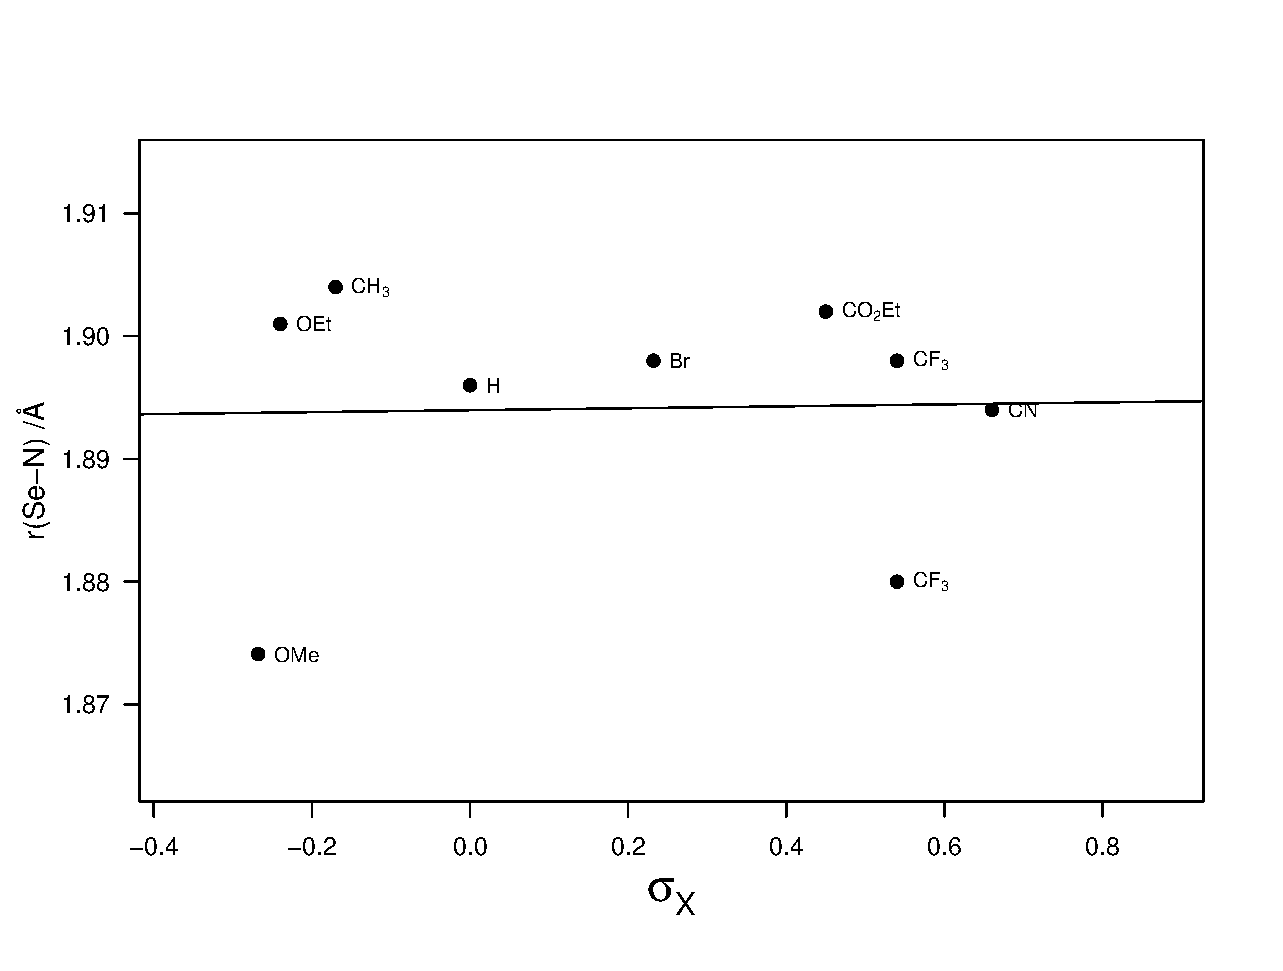
\includegraphics[width=0.9\linewidth]{Figures/hammett-endo-free.eps}
    \caption{Hammett plot of endocyclic \ce{Se-N} bond length of uncomplexed ebselen derivatives.}
    \label{fig:hammett-endo-free}
\end{figure}

The structural effects most relevant to Ch-bonding will manifest themselves in the vicinity of the selenium atom.
Of particular interest is the endocyclic \ce{Se-N} bond length, which serves as a measure of $\sigma^\star$(\ce{Se-N}) orbital occupancy, thus the degree of hyperconjugation and strength of the Ch-bond.

As can be seen in \cref{fig:hammett-endo-free}, there is practically no correlation between the electronic properties of the aryl ring and the endocyclic \ce{Se-N} bond length in crystals of the unbound ebselen derivatives.
This is not unexpected, as in all cases the crystals consist of one dimensional chains of ebselen molecules Ch-bonded to the carbonyl oxygen of the next (\cref{fig:ebs-packing}).
As the magnitude of the $\sigma$-hole (Ch-bond donor ability) is \emph{increased} by an electron withdrawing substituent, the Ch-bond acceptor ability of the carbonyl is \emph{decreased}.
These opposing effects appear to be approximately equal in magnitude, so cancel each other out and give a very flat and featureless Hammett plot.

\begin{figure}
  \centering
  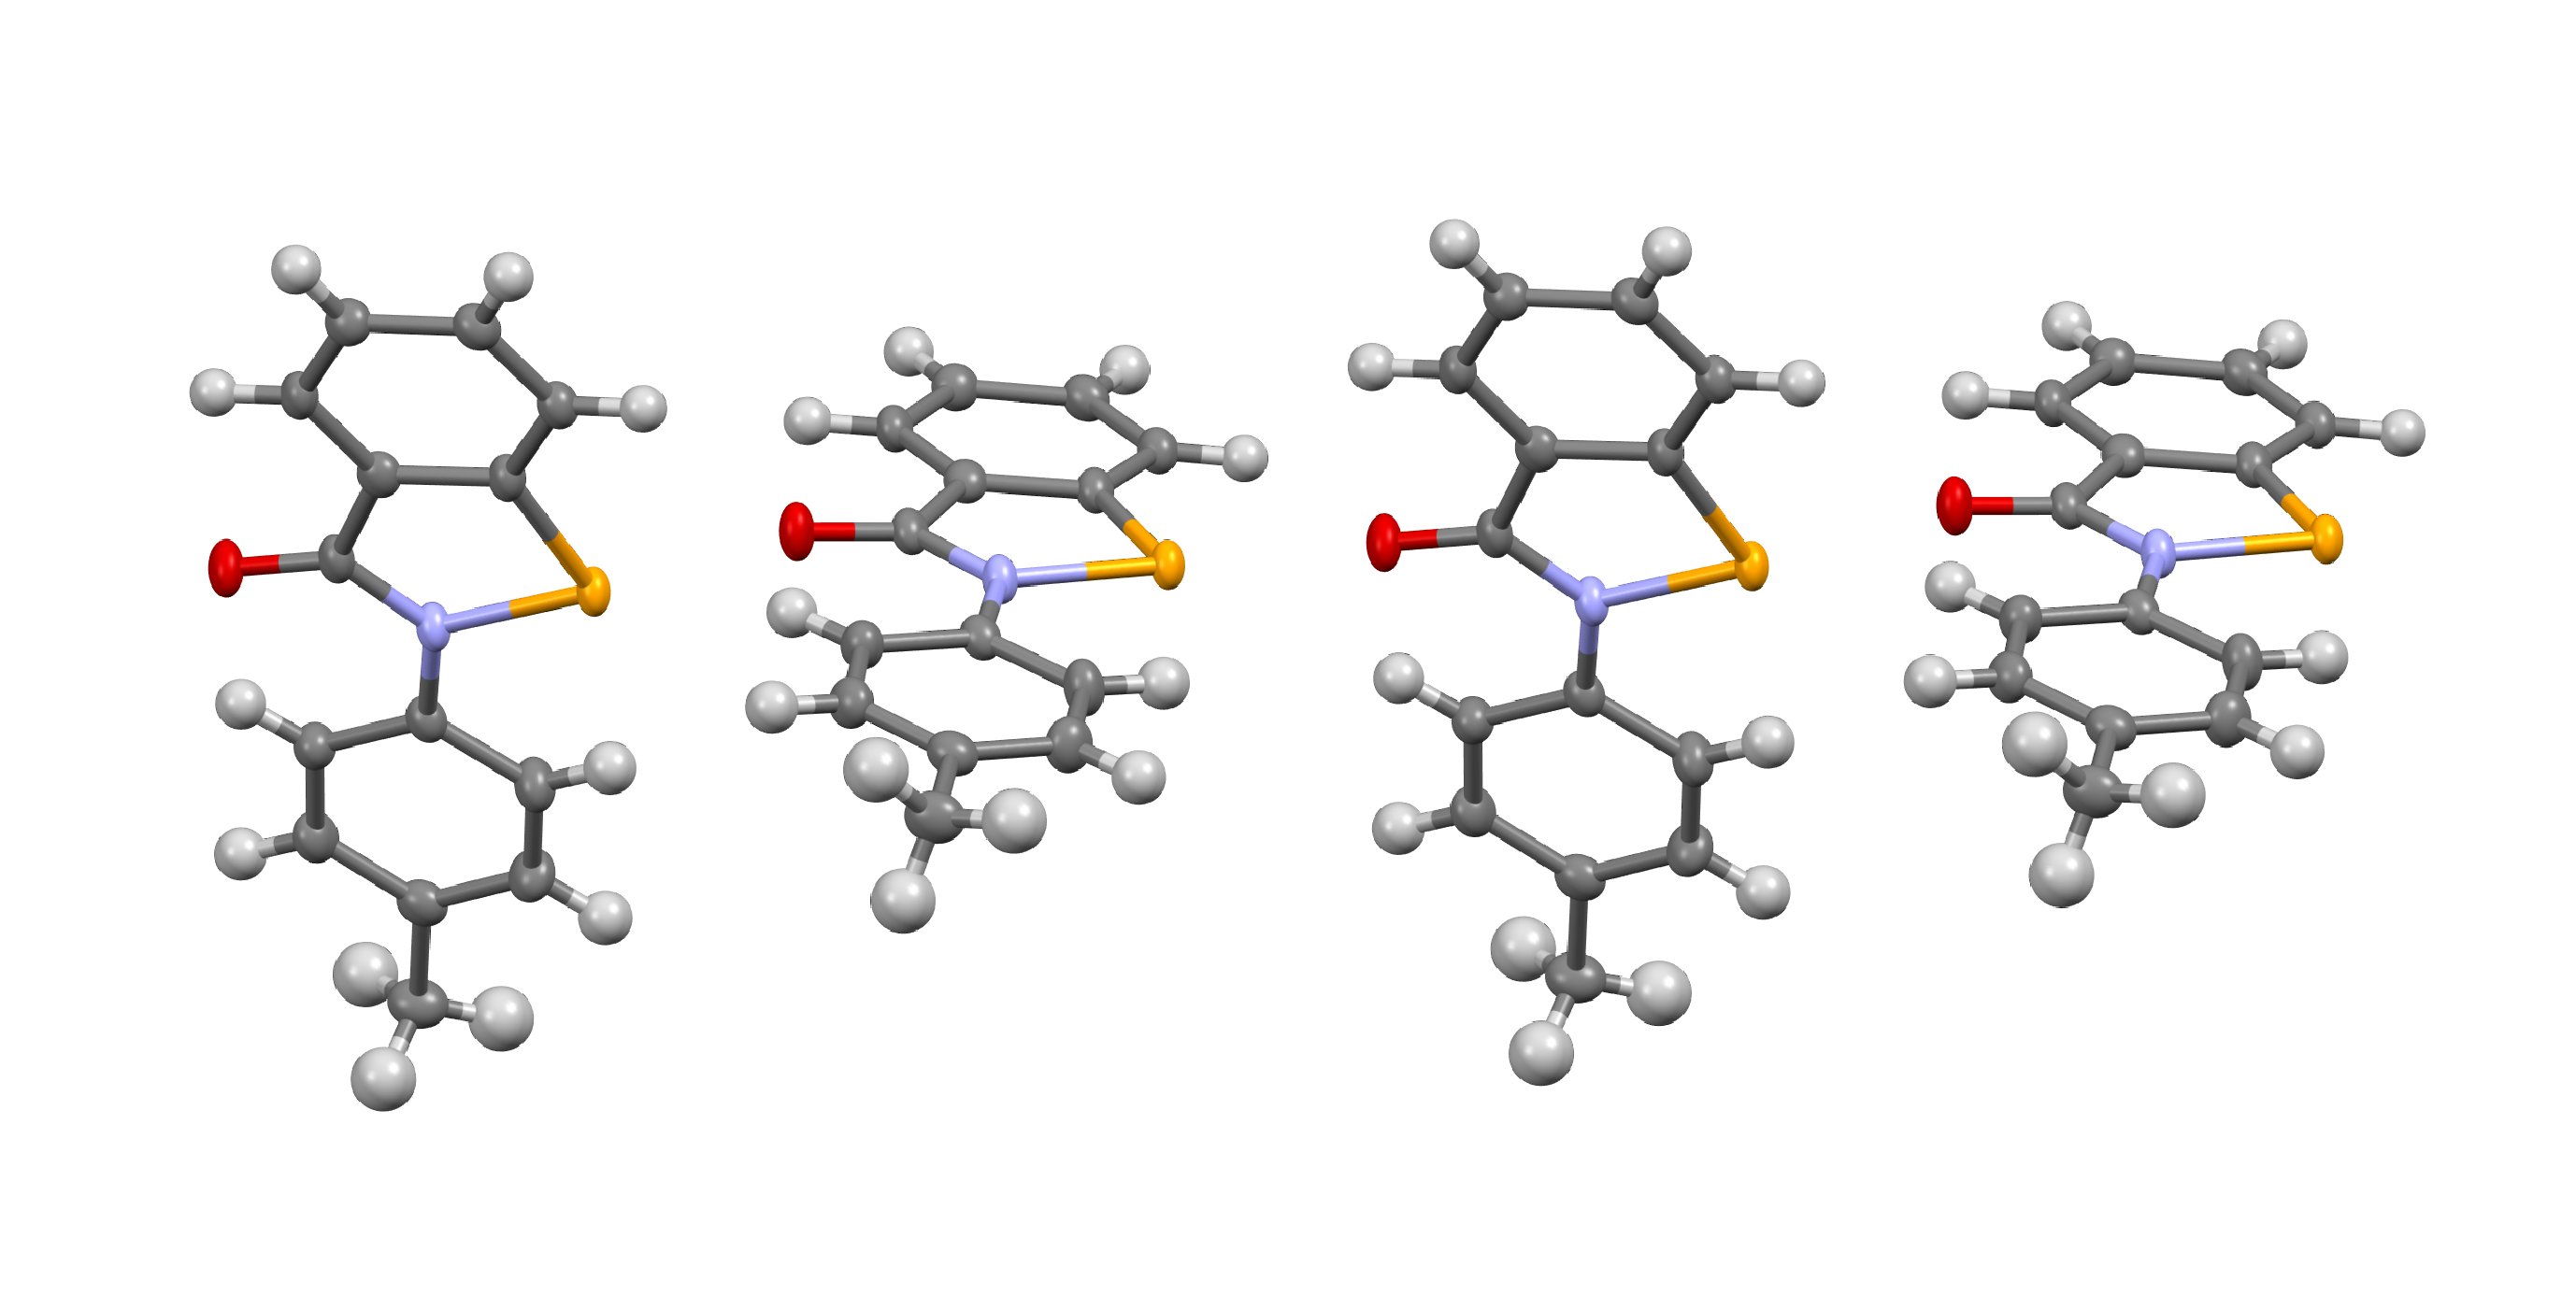
\includegraphics[width=0.6\linewidth]{Figures/ebs.me-packing.pdf}
  \caption{One dimensional chains formed by Ch-bonding between the selenium and carbonyl oxygen in \refcmpd{ebs.4me}. All other ebselen derivatives display a similar packing motif.}
  \label{fig:ebs-packing}
\end{figure}

Fortunately, inspecting the same bond length in co-crystals of ebselen derivatives and a Lewis base gives us a much clearer dependence, as can be seen in \cref{fig:hammett-dmap}, \cref{fig:hammett-pyrrol}, and \cref{fig:hammett-morph}. 
This is because the Ch-bond acceptor ability is now independent of the electronic properties of the Ch-bond donor, so the \ce{Se-N} bond length is determined solely by the latter.
Linear regression analysis affords the relationship $\mathrm{r}(\ce{Se-N}) = (1.957(5) + 0.054(12) \times \sigma_{\mathrm{X}})$~\AA~with a correlation coefficient of 0.6297 for co-crystals with DMAP. 

An inverse correlation can be seen in the \ce{Se\cdots N} Ch-bond length in \cref{fig:hammett-dmap}. 
The gradient of the line is now negative and somewhat steeper, at $-0.15(4)$~\AA.
However the correlation coefficient is decreased to 0.5056.
The reason for this is apparent in the left hand side of the plot.
While the more strongly Ch-bonded systems (with electron withdrawing substituents) are generally very well described by the regression model, the electron rich derivatives \cmpd{ebs.4ome,ebs.4oet} vary significantly in their bond lengths.\footnote{This is also visible, though less apparent, in the plot of endocyclic bond lengths (\cref{fig:hammett-dmap}).}
Indeed, omitting these data points improves the correlation coefficient to 0.8148 while the gradient and intercept are almost unchanged at $-0.156(28)$~\AA~and $2.386(15)$~\AA~respectively, suggesting that the model is appropriate, and that there is some other effect occurring in electron rich systems.

\begin{figure}
    \centering
    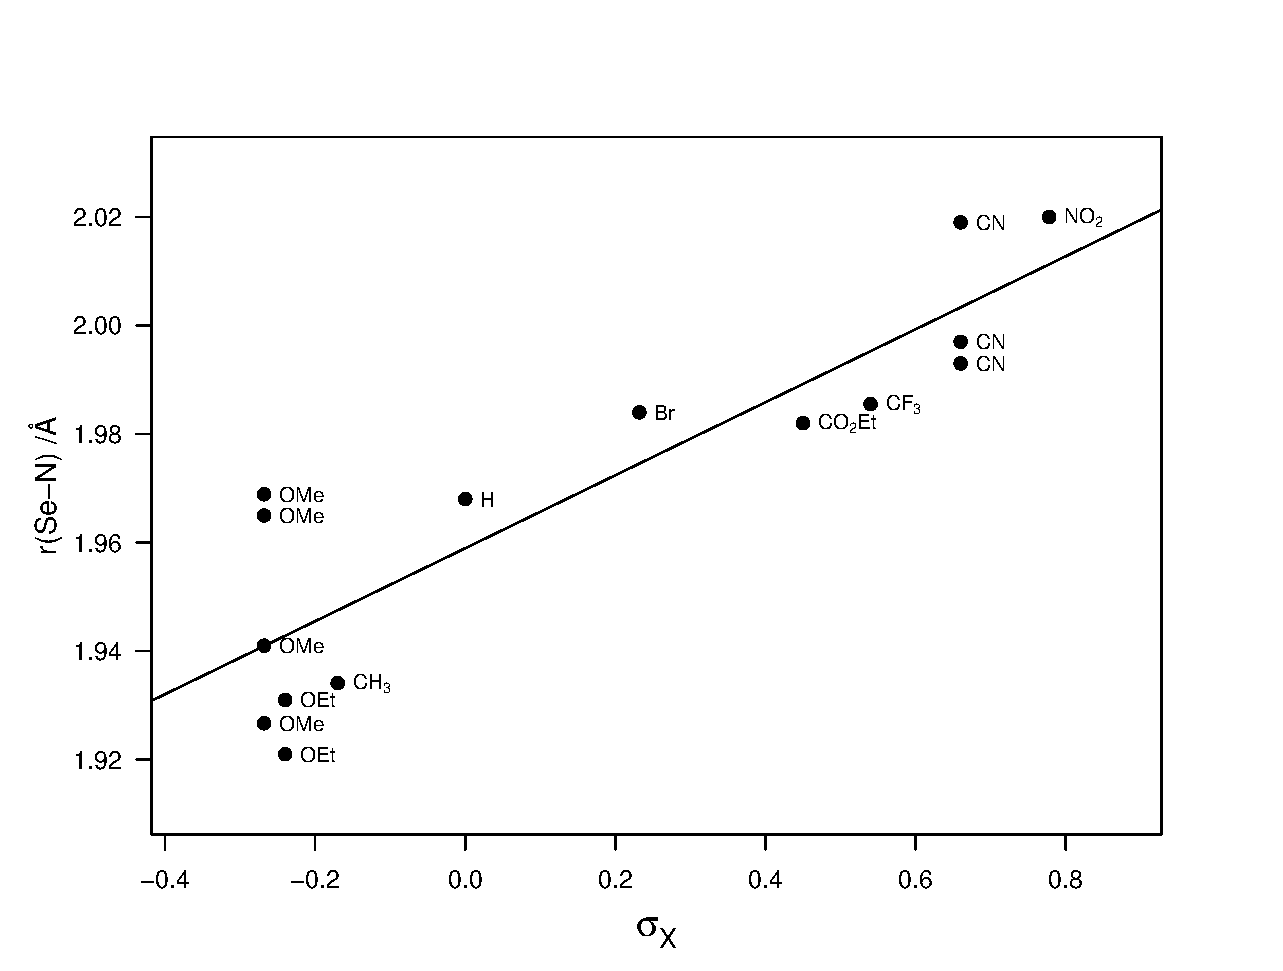
\includegraphics[width=0.45\linewidth]{Figures/hammett-endo-dmap.eps}
    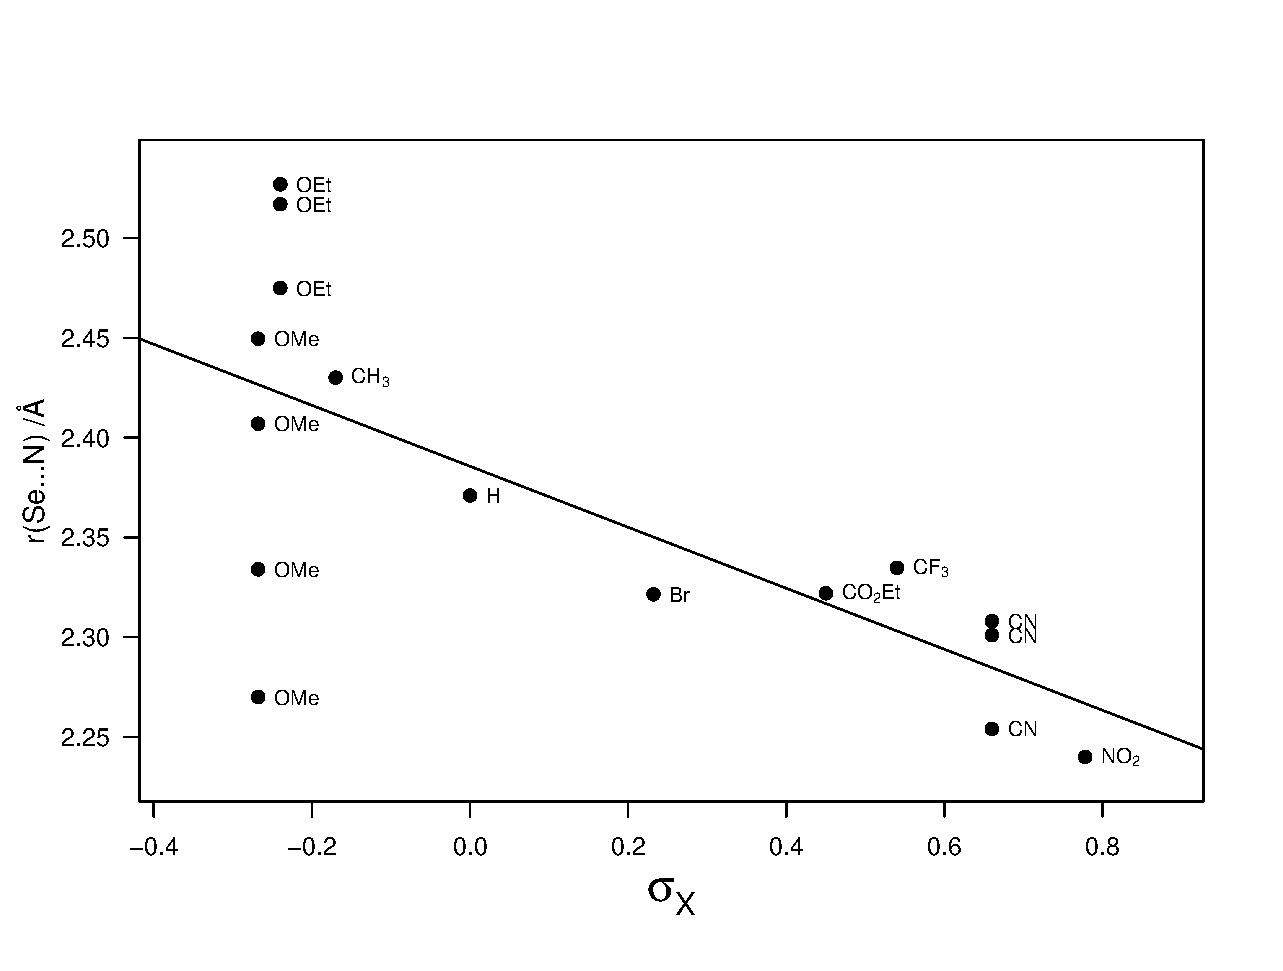
\includegraphics[width=0.45\linewidth]{Figures/hammett-dmap.eps}
    \caption{Hammett plots of endocyclic \ce{Se-N} bond length and \ce{Se\cdots N} Ch-bond length of ebselen derivatives complexed with DMAP. The lines are described by the equations $\mathrm{r}(\ce{Se-N}) = (1.957(5) + 0.054(12) \times \sigma_{\mathrm{X}})$~\AA~ and $\mathrm{r}(\ce{Se\cdots N}) = (2.385(17) - 0.15(4) \times \sigma_{\mathrm{X}})$~\AA.}
    \label{fig:hammett-dmap}
\end{figure}

\begin{figure}
  \centering
  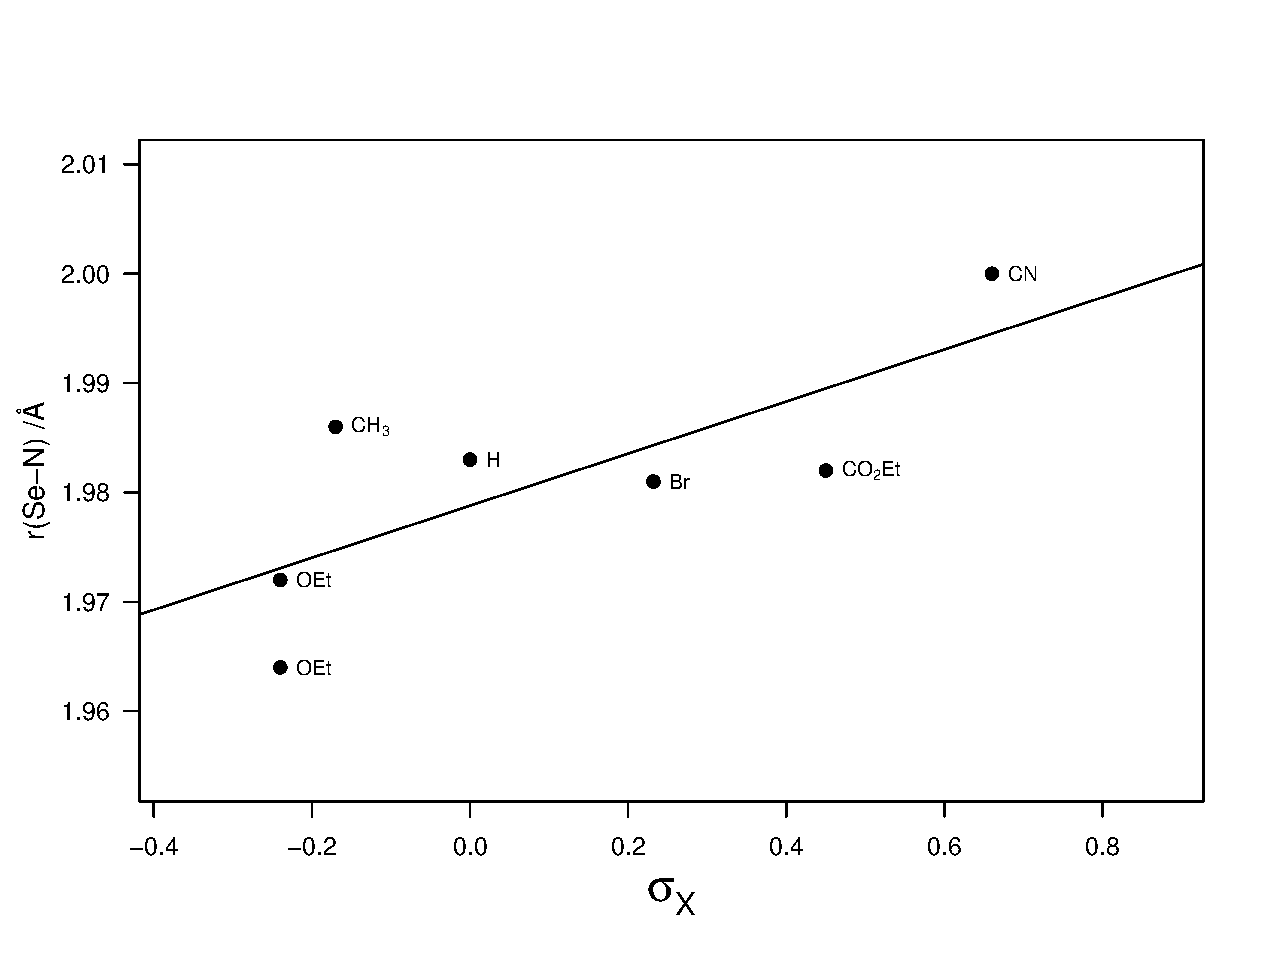
\includegraphics[width=0.45\linewidth]{Figures/hammett-endo-pyrrol.eps}
  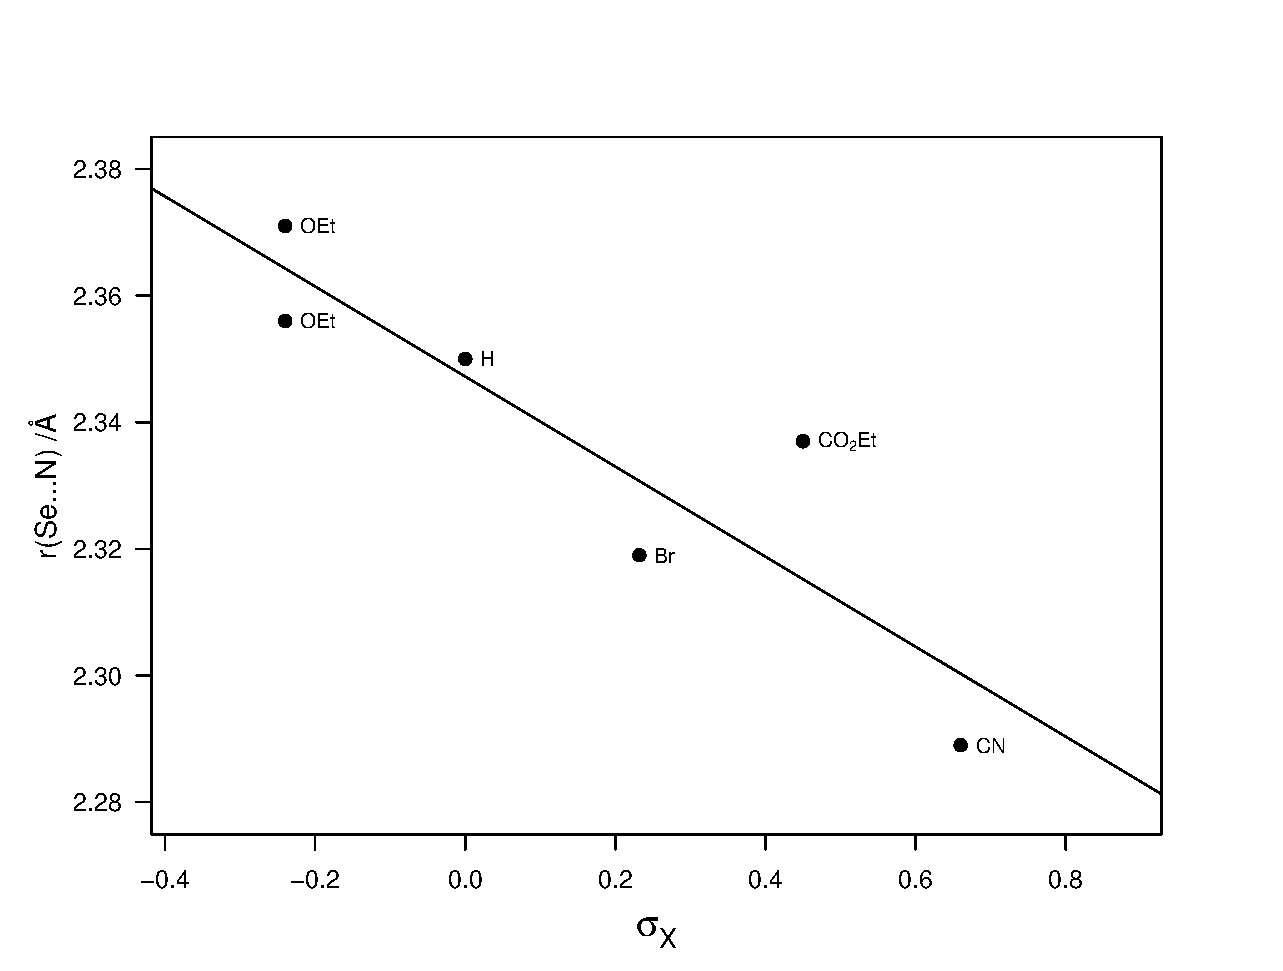
\includegraphics[width=0.45\linewidth]{Figures/hammett-pyrrol.eps}
  \caption{Hammett plots of endocyclic \ce{Se-N} bond length and \ce{Se\cdots N} Ch-bond length of ebselen derivatives complexed with \refcmpd{py.pyrrol}. The lines are described by the equations $\mathrm{r}(\ce{Se-N}) = (1.9788(32) - 0.024(9) \times \sigma_{\mathrm{X}})$~\AA~($R^2=0.5722$) and $\mathrm{r}(\ce{Se-N}) = (2.331(14) - 0.04(4) \times \sigma_{\mathrm{X}})$~\AA~($R^2=0.1588$)}
  \label{fig:hammett-pyrrol}
\end{figure}

\begin{figure}
  \centering
  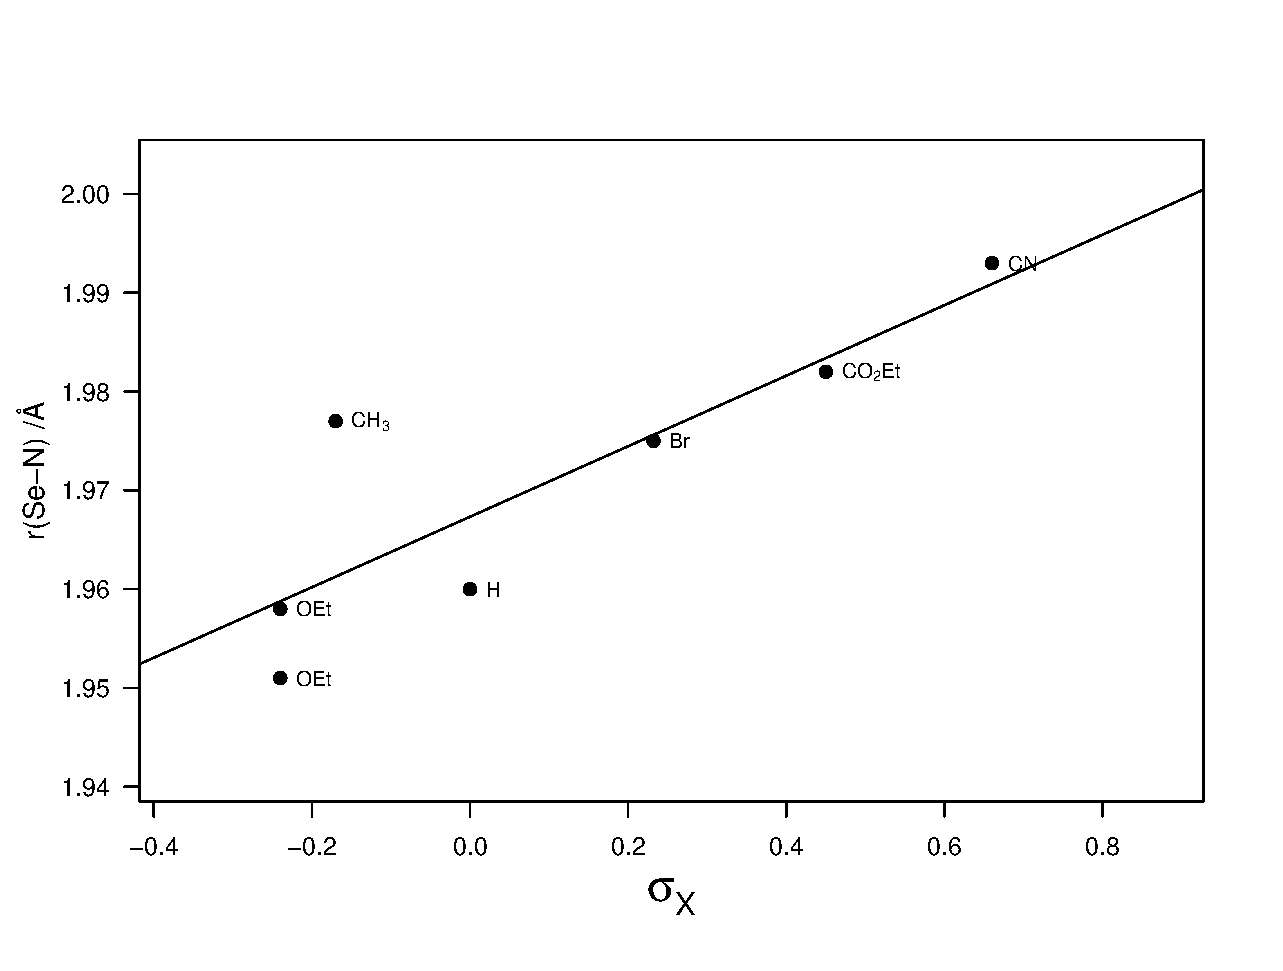
\includegraphics[width=0.45\linewidth]{Figures/hammett-endo-morph.eps}
  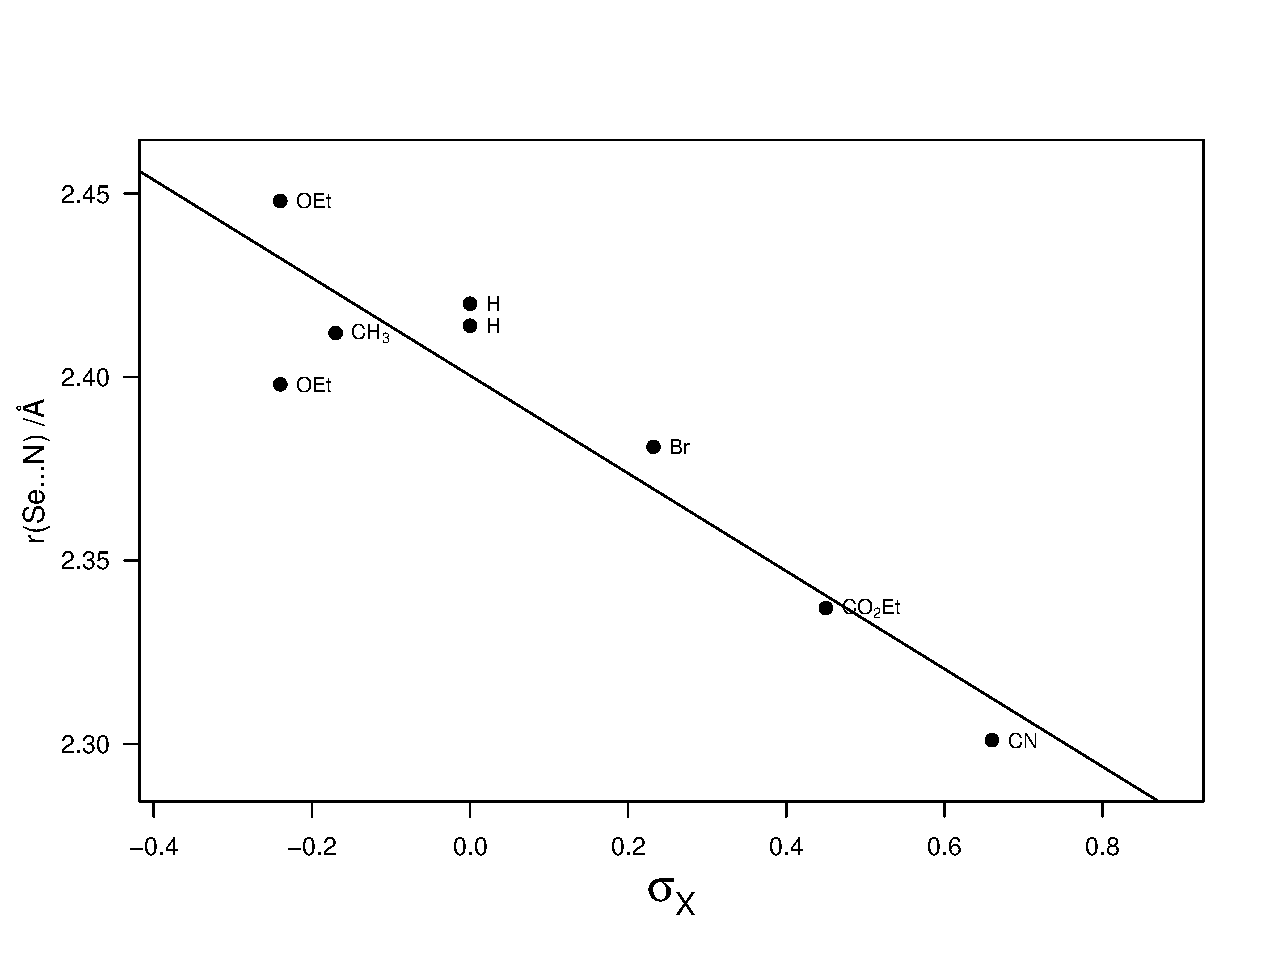
\includegraphics[width=0.45\linewidth]{Figures/hammett-morph.eps}
  \caption{Hammett plots of endocyclic \ce{Se-N} bond length and \ce{Se\cdots N} Ch-bond length of ebselen derivatives complexed with \refcmpd{py.morph}. The line is described by the equation $\mathrm{r}(\ce{Se-N}) = (1.9673(34) - 0.035(10) \times \sigma_{\mathrm{X}})$~\AA~($R^2=0.7260$) and $\mathrm{r}(\ce{Se-N}) = (2.397(77) - 0.13(2) \times \sigma_{\mathrm{X}})$~\AA~($R^2=0.8708$).}
  \label{fig:hammett-morph}
\end{figure}

\subsubsection{Co-crystals where \texorpdfstring{$Z^\prime=2$}{Z'=2}}
DFT calculations show that the vibrational mode associated with Ch-bond stretching is found at very low energy.
The force constant is 5--10~$\mu$dyne$\cdot$\AA$^{-1}$, which means that the energetic penalty associated with a 0.18~\AA~ deformation (the difference between the shortest and longest Ch-bond length) is only 0.02--0.03~kcal$\cdot$mol$^{-1}$.
Crystal packing forces (the sum of weak interactions such as C-H/$\pi$, $\pi /\pi$ and C-H/O interactions) are commonly accepted to be in the range of 1--2~kcal$\cdot$mol$^{-1}$, so it is perhaps not surprising that the Ch-bond is deformed by the crystal environment.\autocite{Dunitz1988}

That said, there are no obvious differences between the two Ch-bond environments in any of the crystals that display this effect.
We performed a solid state IR experiment to probe the crystalline environment surrounding the carbonyl, which is dependent on the Ch-bond environment due to conjugation through the amidic nitrogen (\cref{fig:ebs-4oet-dmap-ir}).

\begin{figure}
    \centering
    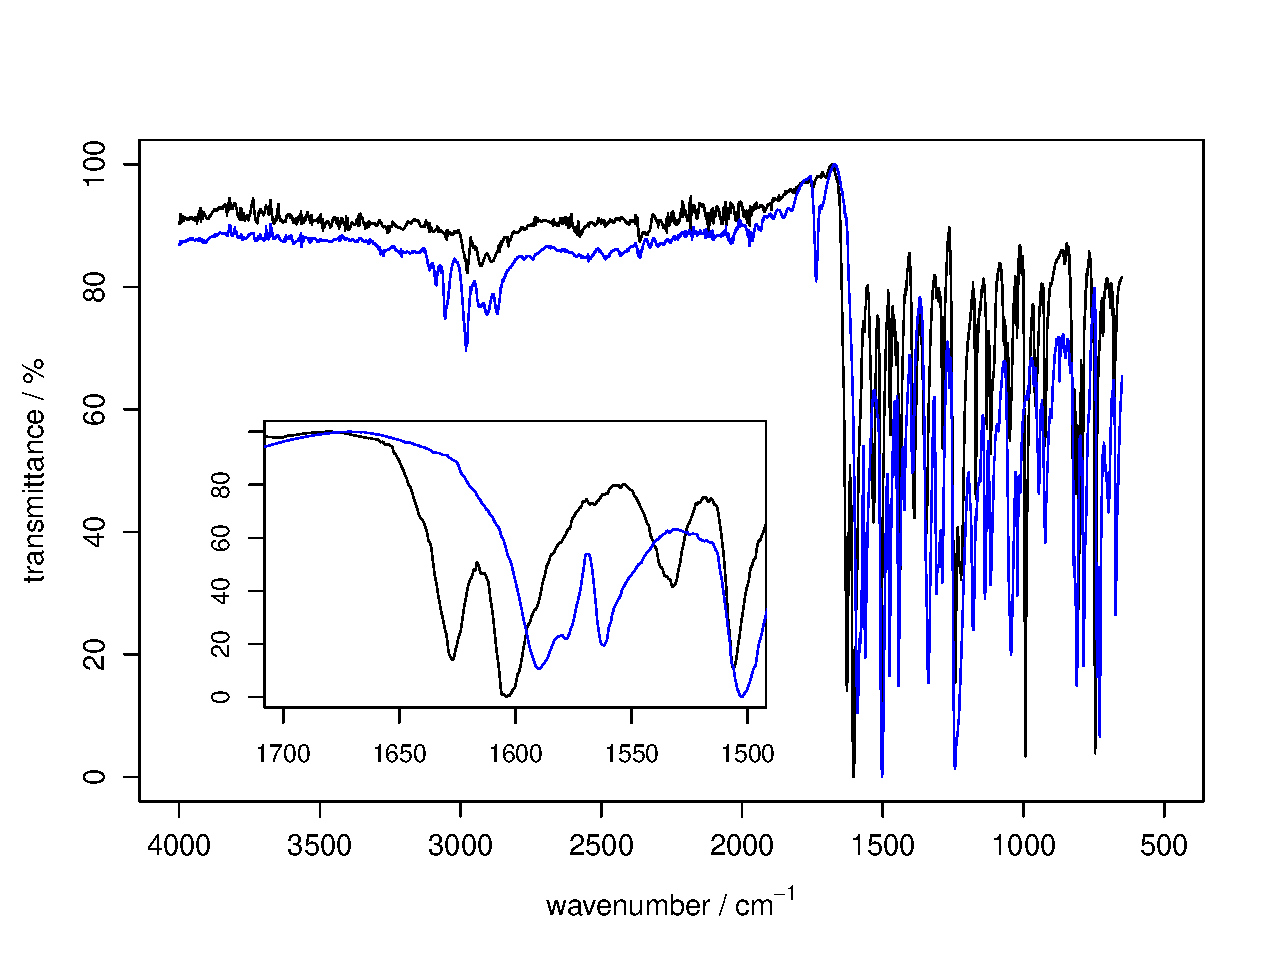
\includegraphics[width=0.9\linewidth]{Figures/ebs-4oet-dmap-ir.eps}
    \caption{Solid state IR spectrum of \refcmpd{ebs.4oet}$\cdot$DMAP. The spectrum of the pure \refcmpd{ebs.4oet} is shown in gray.}
    \label{fig:ebs-4oet-dmap-ir}
\end{figure}

In the pure compound the carbonyl peak is found at approximately 1590~cm$^{-1}$ and is relatively sharp and well defined.
In the co-crystal, we observe the carbonyl peak at higher wavenumber (1610~cm$^{-1}$), due to the increased double bond character, as the $\pi$ system and oxygen lone pair are no longer involved in the Ch-bond.
This effect ostensibly outweighs the \emph{decreased} double bond character caused by the shortened Ch-bond formed between the pyridyl nitrogen and selenium (\cref{fig:ch-bond-deloc}).

\begin{figure}
    \centering
    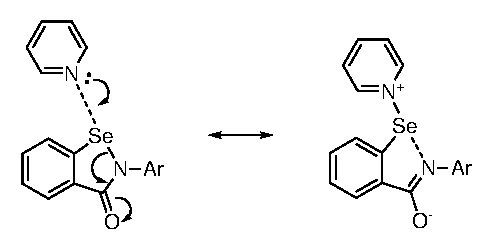
\includegraphics[scale=0.8]{Figures/ch-bond-deloc.eps}
    \caption{Contributing resonance form of a Ch-bonded complex with strong Lewis bases. The double bond character of the carbonyl is decreased.}
    \label{fig:ch-bond-deloc}
\end{figure}

If there are truly two Ch-bonded environments, we would expect to see splitting or at least broadening of the carbonyl signal in the IR spectrum of the co-crystal.
This is not the case, meaning that either the difference is too small to be seen in the spectrum, or the two environments are actually the same, and the measured differences are a crystallographic artefact, either a manifestation of missed symmetry, disorder, or a doubled cell.

However, we do not believe this is likely, for two reasons.
Firstly, the data was of extremely high quality, and no alerts were raised in the ADDSYM routine of PLATON.
Secondly, a refinement was conducted with a tight SADI restraint on the Ch-bonds ($\sigma=0.0001$), which forced them to adopt the same length of approximately 1.949~\AA.
This increased the R-factor by 1.2\%, and significant residual density was visible where the pyridyl nitrogen had been displaced.
Furthermore, removal of the restraint recovered the original model, ruling out the possibility of a false minimum.

Solid state NMR of the co-crystal was also used to investigate the crystalline environment.
A sample of \cmpd{ebs.4ome}$\cdot$DMAP was first characterised by single crystal x-ray diffraction, which confirmed the polymorph and structural parameters (\cref{fig:ebs-4ome-dmap-xray}).

\begin{figure}
  \centering
  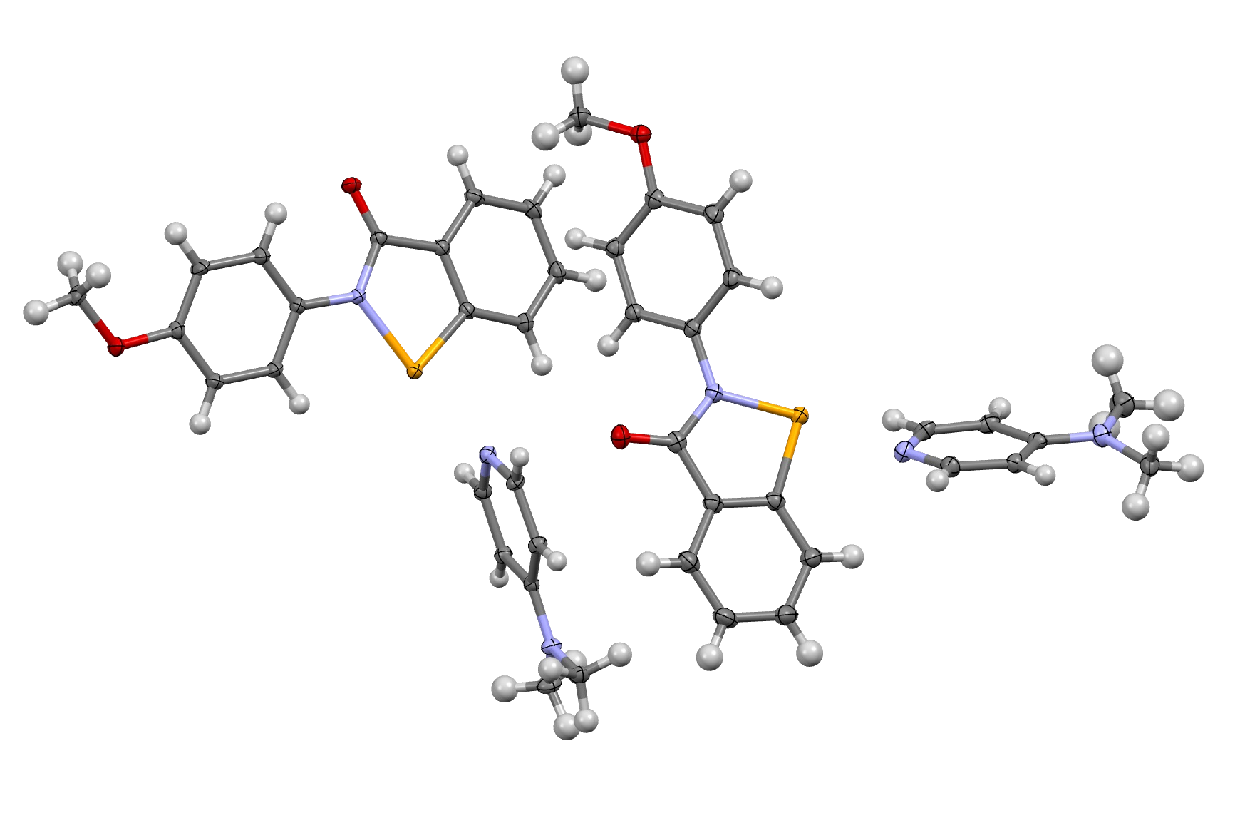
\includegraphics[width=0.8\linewidth]{Figures/ebs-4ome-dmap-xray.pdf}
  \caption{Single crystal x-ray structure of \refcmpd{ebs.4ome}$\cdot$DMAP, displaying the two systems in the asymmetric unit.}
  \label{fig:ebs-4ome-dmap-xray}
\end{figure}

The bulk material was then crushed and homogenised, and characterised by powder x-ray diffraction.
The measured powder pattern was in excellent agreement with the pattern calculated from the single crystal data (\cref{fig:ebs-4ome-dmap-pdx}), indicating good phase purity.

\begin{figure}
    \centering
    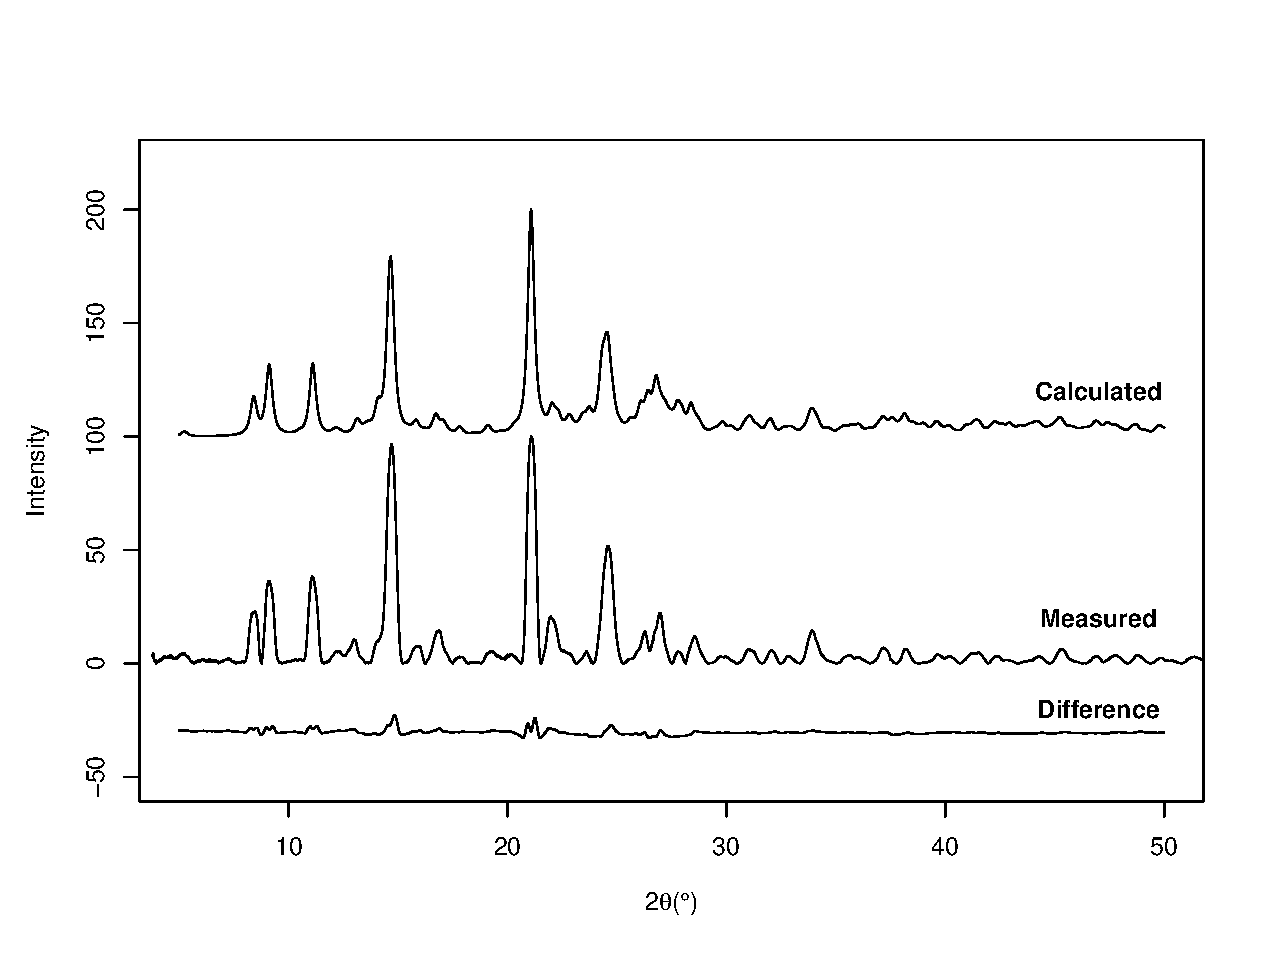
\includegraphics[width=0.9\linewidth]{Figures/ebs-4ome-dmap-pdx.eps}
    \caption{Calculated vs measured powder diffraction pattern for \refcmpd{ebs.4ome}$\cdot$DMAP.}
    \label{fig:ebs-4ome-dmap-pdx}
\end{figure}

Spectra were then acquired using a 400~MHz instrument and triple resonance MAS room temperature probe tuned to \ce{^1H}, \ce{^{13}C} and  \ce{^{77}Se}.
\ce{^1H}--\ce{^{13}C} or \ce{^1H}--\ce{^{77}Se} cross polarisation was used for signal enhancement, and a spin frequency of 10~kHz was used in most cases.

\ce{CDCl3} solution spectra of the complex were also obtained on a 500~MHz instrument.
The \ce{^1H} and \ce{^1H}--\ce{^{13}C} HSQC spectra (\cref{fig:ebs-4ome-dmap-sol}) were used to unambiguously assign the \ce{^{13}C} spectrum.

\begin{figure}
    \centering
    \begin{subfigure}[t]{\linewidth}
    \centering
    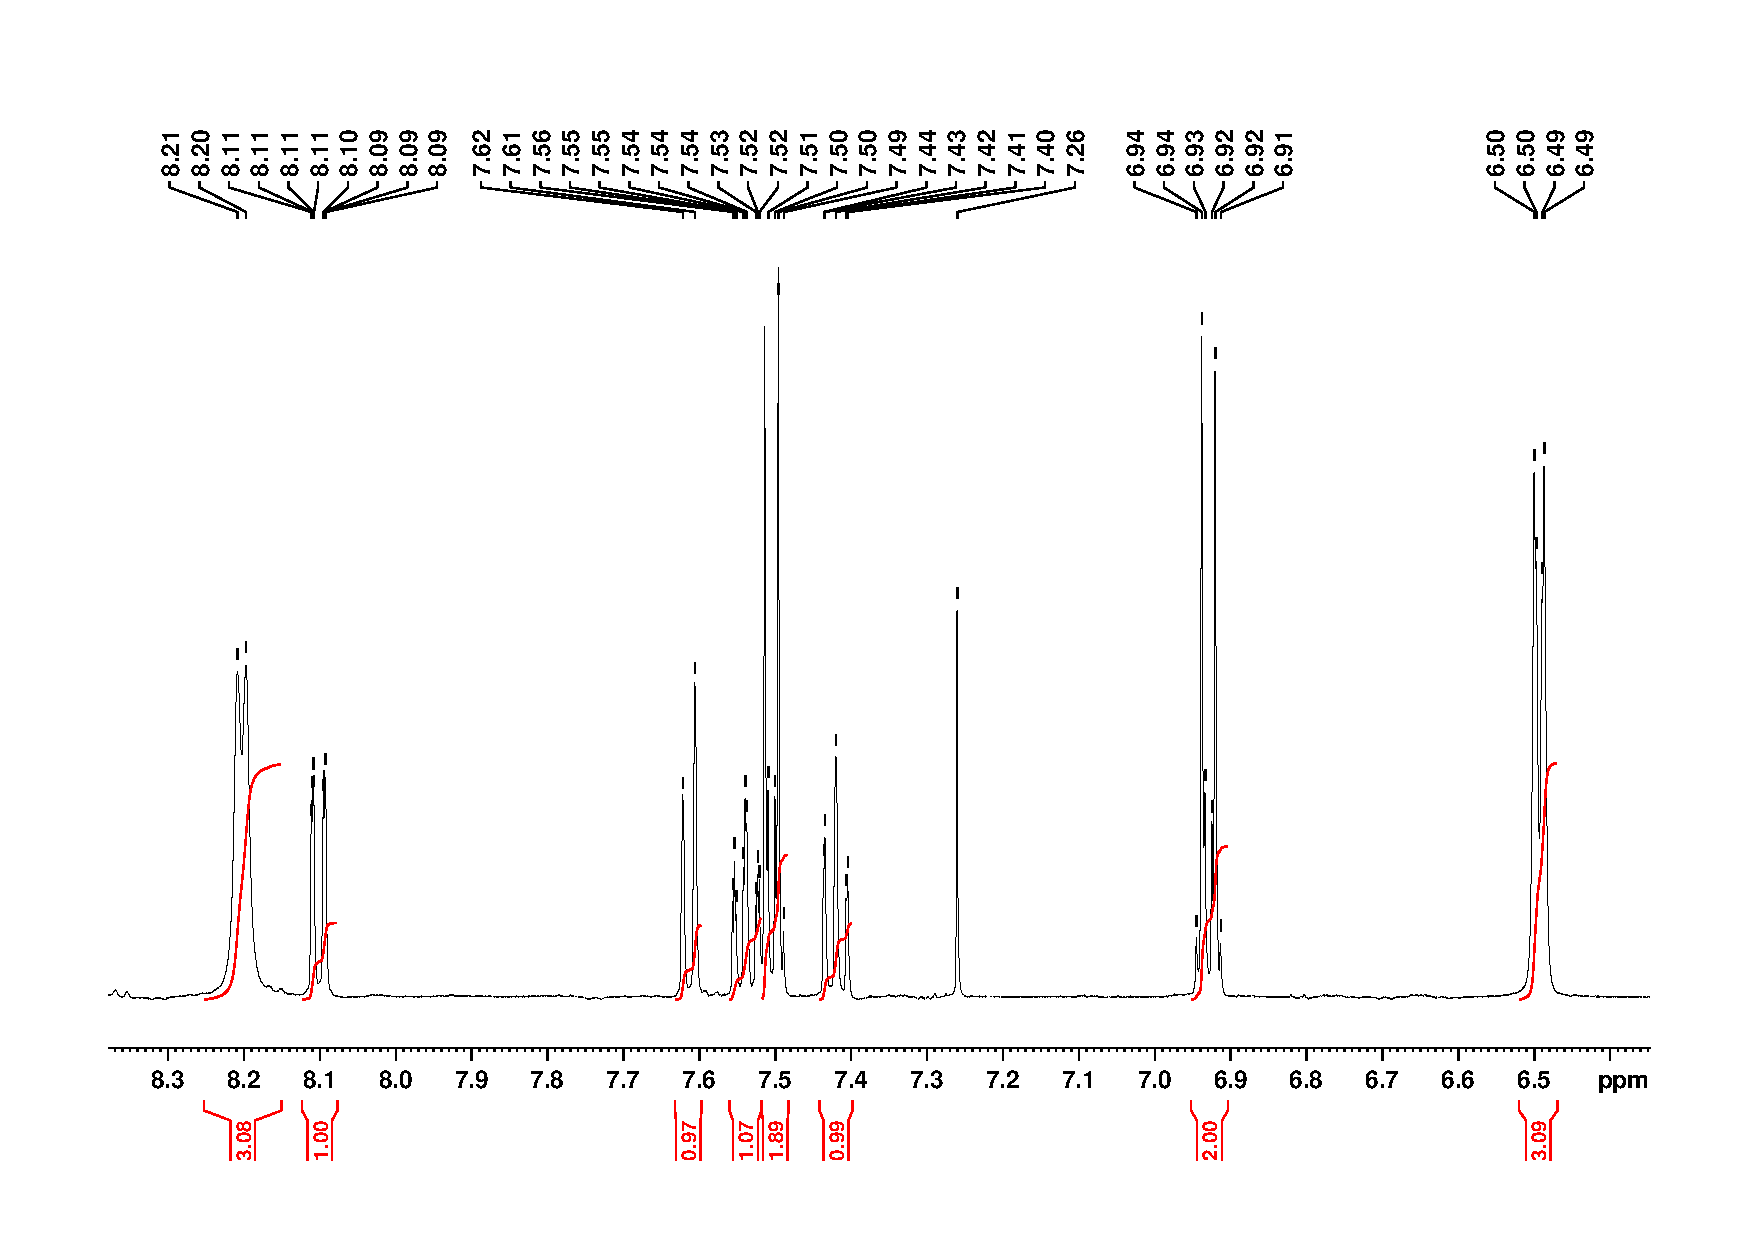
\includegraphics[width=\linewidth]{Figures/ebs-4ome-dmap-sol-1h.pdf}
    \caption{Solution \ce{^1H} spectrum of \refcmpd{ebs.4ome}$\cdot$DMAP}
    \label{fig:ebs-4ome-dmap-sol-1h}
    \end{subfigure}
    
    \begin{subfigure}[t]{\linewidth}
    \centering
    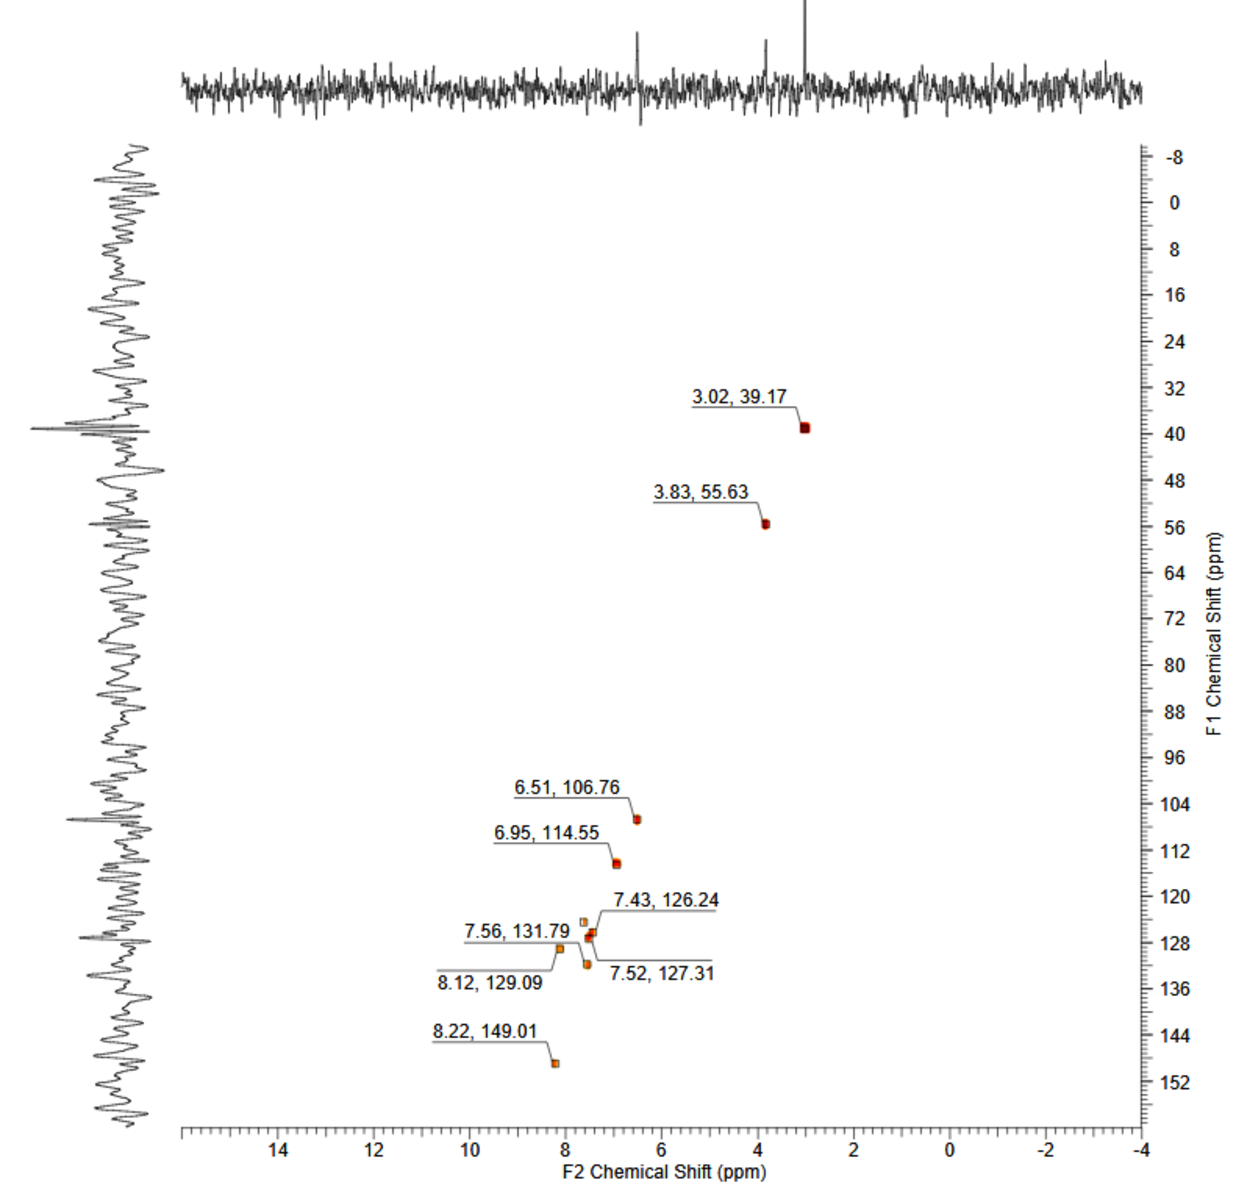
\includegraphics[width=0.8\linewidth]{Figures/ebs-4ome-dmap-sol-hsqc.pdf}
    \caption{Solution \ce{^1H}-\ce{^{13}C} HSQC spectrum of \refcmpd{ebs.4ome}$\cdot$DMAP}
    \label{fig:ebs-4ome-dmap-sol-hsqc}
    \end{subfigure}
    \caption{}
    \label{fig:ebs-4ome-dmap-sol}
\end{figure}

The aromatic region of the solid state \ce{^{13}C} spectrum is shown in \cref{fig:cpmas-sol-13c}, overlaid with the corresponding solution spectrum\footnote{The \ce{^{13}C} spectrum was referenced to adamantane.}.
Good agreement is observed for all signals, with some interesting phenomena visible in the solid state spectrum.
Firstly, the signal at 138.62~ppm corresponding to C8 is split into a 1:1:1 triplet, possibly due to coupling to the spin 1 \ce{^{14}N} nucleus adjacent.
However this is not observed for the C7 signal, nor any signals in the pyridyl ring.
Secondly, shoulders can be seen on the C15/C19 and C16/C18 signals.
This indicates that the crystalline environment surrouding each DMAP is different, which provides further evidence that there are indeed two systems in the asymmetric unit.
The relatively poor resolution of the solid state \ce{^{13}C} NMR spectrum limits further analysis, particularly of the C1 signal which is obscured by several other signals.

\begin{figure}
    \centering
    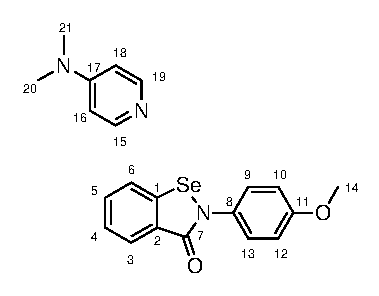
\includegraphics[scale=0.8]{Figures/numbering.eps}
    
    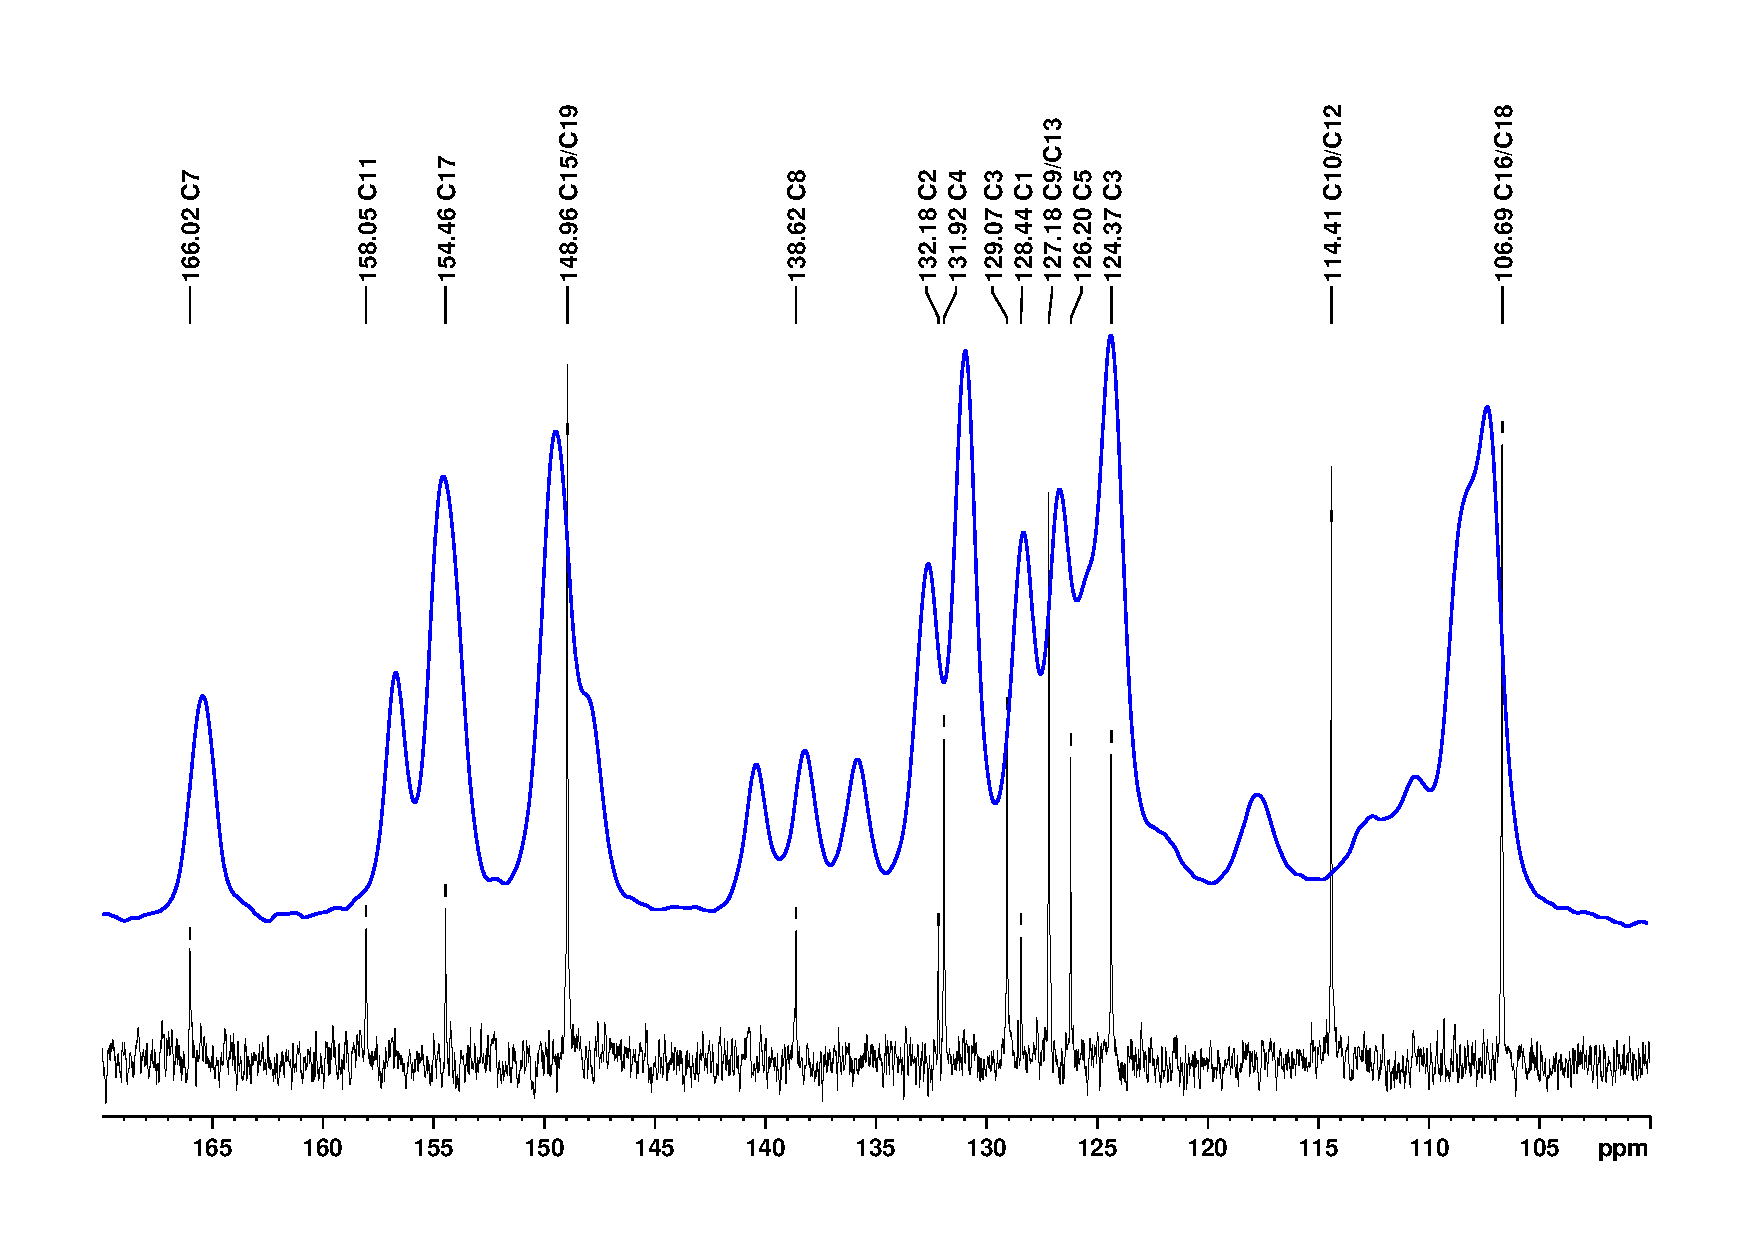
\includegraphics[width=\linewidth]{Figures/ebs-4ome-dmap-cpmas-sol-13c.pdf}
    \caption{Solid state \ce{^{13}C}-NMR spectrum of \refcmpd{ebs.4ome}$\cdot$DMAP (blue) overlaid on solution spectrum of the same (black). Signals are assigned according to the numbering scheme above.}
    \label{fig:cpmas-sol-13c}
\end{figure}

To conclusively demonstrate that there are two systems in the asymmetric unit we conducted a solid state \ce{^{77}Se} NMR experiment, which is shown in \cref{fig:cpmas-sol-77se}.\footnote{The \ce{^{77}Se} spectrum was referenced to diphenyl diselenide.}
In solution, the \ce{^{77}Se} resonance is found around 900~ppm relative to dimethylselenide ($\delta=$0~ppm), and appears as one singlet due to the averaging of all environments.
In the solid phase, the spectrum is significantly more complex, primarily due to chemical shift anisotropy which manifests as spinning sidebands.
The true anisotropic chemical shifts can only be discerned by varying the MAS spinning speed, which changes the spacing of the sidebands while leaving the parent signals in the same place.
Spinning at 12~kHz instead of 10~kHz showed that the signals at 834.69 and 867.02~ppm are the true isotropic chemical shifts, and the fact that there are two signals show that there are indeed two Ch-bonded systems in the asymmetric unit.

\begin{figure}
    \centering
    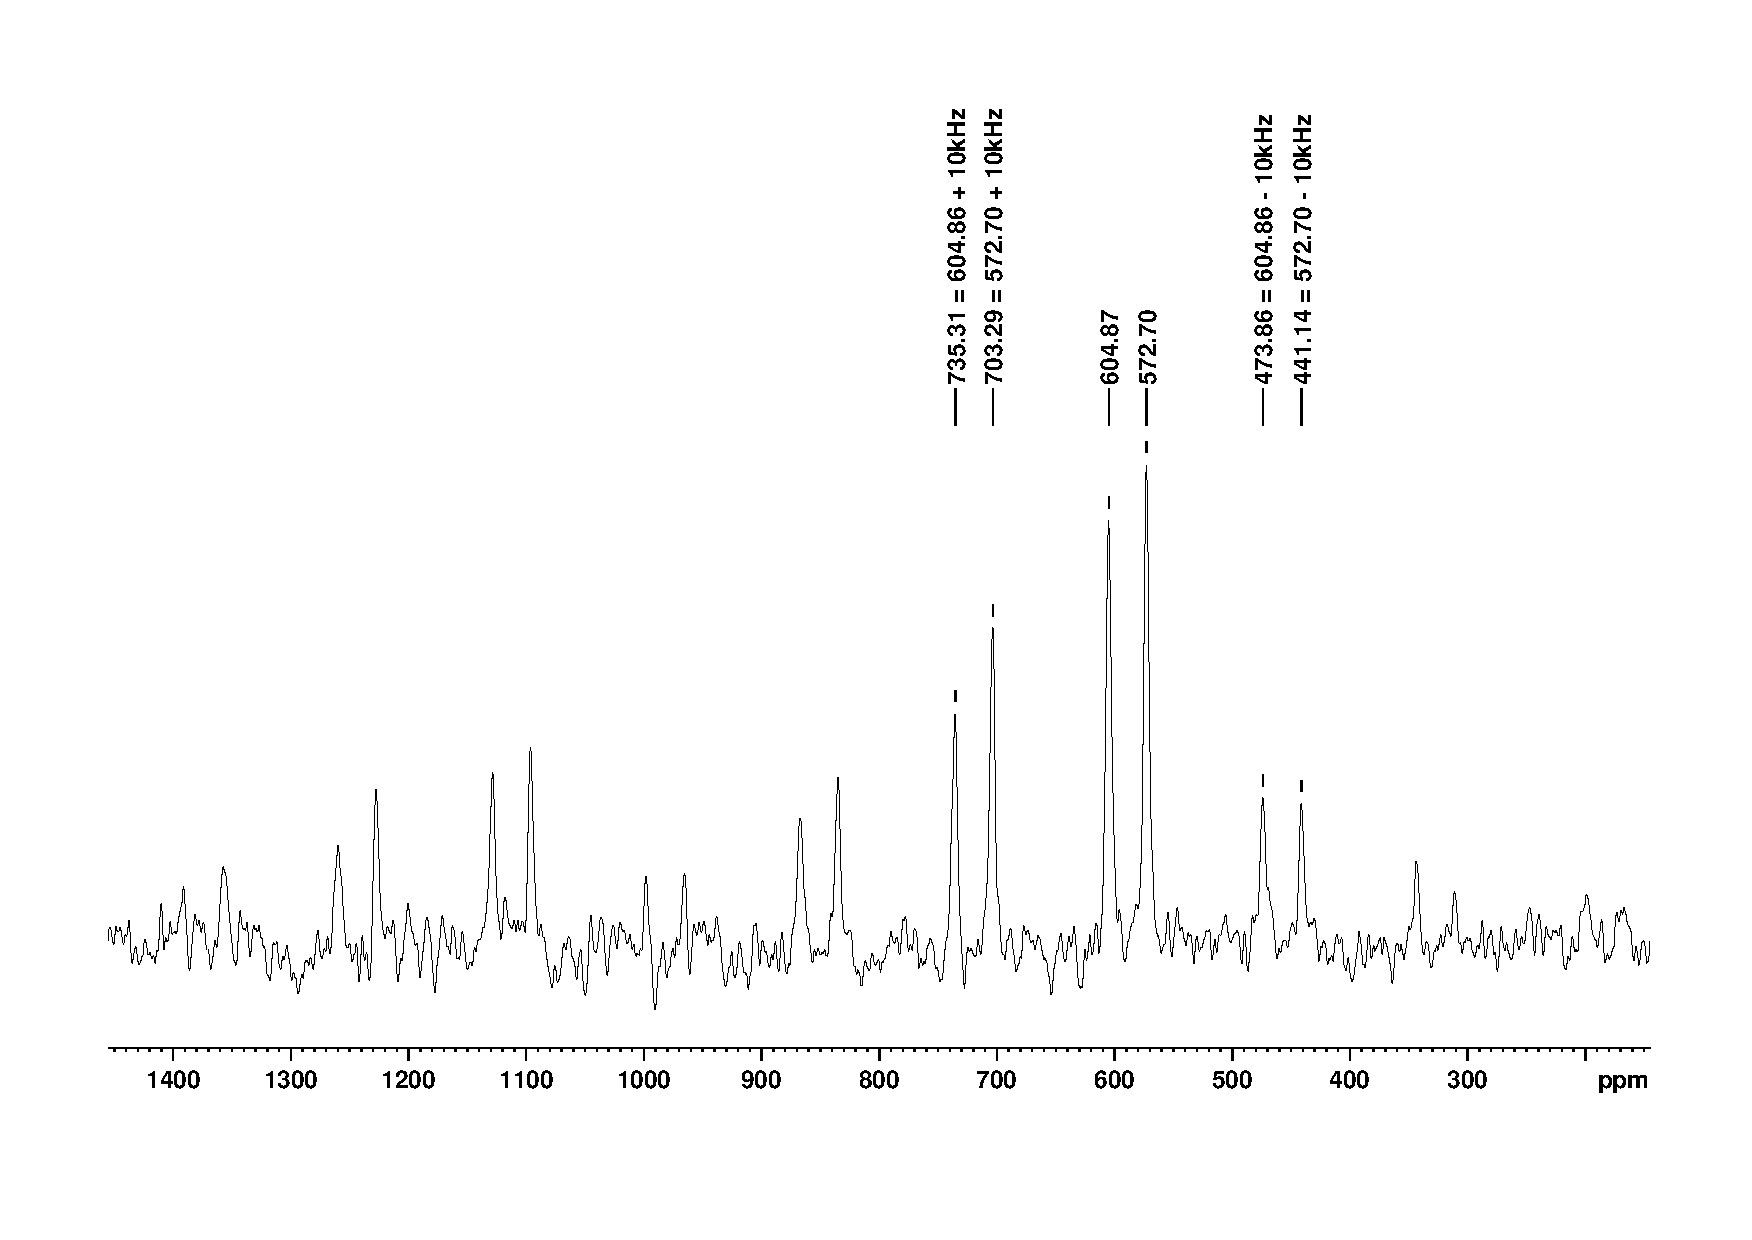
\includegraphics[width=0.7\linewidth]{Figures/ebs-4ome-dmap-cpmas-77se.pdf}
    \caption{Solid state \ce{^{77}Se}-NMR spectrum of \refcmpd{ebs.4ome}$\cdot$DMAP. The primary resonances are visible at 834.69 and 867.02~ppm. The remaining peaks are spinning sidebands, and are separated from the parent signals by multiples of 10~kHz (the magic angle spinning frequency).}
    \label{fig:cpmas-sol-77se}
\end{figure}

\subsubsection{SOME MORE ABOUT HAMMETT STUFF}

\subsection{Measurement of chemical shift anisotropy}
The chemical shift of a nucleus is not a simple scalar quantity, as solution phase NMR experiments might suggest.
The shielding, and hence the effective magnetic field felt by the nucleus depends on the electronic environment around the nucleus, which is decidedly \emph{an}isotropic, therefore incapable of being expressed as a scalar.
Depending on the orientation of the electron cloud (and other shielding/deshielding influences) around the nucleus with respect to the magnetic field, different chemical shifts will be observed for the same nucleus.
This phenomenon is the chemical shift anisotropy of a nucleus, and it is described mathematically by a second rank tensor, which is geometrically depicted as an ellipsoid.

In a solution phase NMR experiment, rapid and random tumbling of the molecules averages out the anisotropy of each signal, affording a sharp peak at the isotropic chemical shift.
This can be simulated to some degree by magic angle spinning in solids experiments, but it is often the case that the chemical shift anisotropy is more interesting that the isotropic shift, so a solid phase NMR experiment is the only way to examine it.

The shape of the chemical shift tensor can provide insight into the electronic environment of a nucleus, with large shielding components often being aligned with electronic features such as bonds or lone pairs.
It is often convenient to define a principal axis system (PAS) for the tensor, consisting of two components which describe the longest and shortest axes of the ellipsoid, and the axis perpendicular to both.
The PAS of the chemical shielding tensor is denoted by the lowercase $x$, $y$ and $z$, and the components of the tensor which are aligned with these axes are labelled $\sigma_{xx}$, $\sigma_{yy}$ and $\sigma_{zz}$.
The laboratory reference frame is denoted by the uppercase $X$, $Y$ and $Z$, with the magnetic field $B_0$ being aligned with the $Z$ axis.
A common method for transforming one coordinate system to another is through the use of Euler angles $\alpha$, $\beta$ and $\gamma$, which define sequential right-handed rotations about the axes of the rotating frame.
As the chemical shielding is necessarily invariant to rotation about $Z$, we can dispense with the first of these angles $\alpha$, and simply refer to the latter two as the polar angles $\beta = \theta$ and $\gamma = \phi$.
The chemical shielding tensor is thus depicted in \cref{fig:chemical-shielding-tensor}, and this will be the convention used in this work.

\begin{figure}
  \centering
  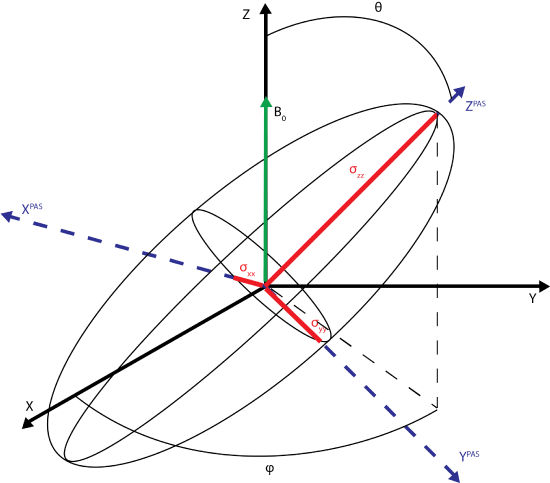
\includegraphics[width=0.4\linewidth]{Figures/Chemical_Shift_Tensor.png}
  \caption{Representation of the principal axis system (PAS, blue dotted lines) with respect to the laboratory reference frame (black solid lines). The polar angles $\theta$ and $\phi$ relate the former to the latter. The principal components of the tensor are shown in red, and the overall shape is shown by the black ellipses.}
  \label{fig:chemical-shielding-tensor}
\end{figure}

In almost all experiments, the chemical shielding tensor $\sigma$ is only indirected measured, \emph{via} the chemical shift $\delta$, which is defined with respect to a reference nucleus such that $\delta = \sigma_{\textrm{ref}} - \sigma_{\textrm{sample}}$.
As the coordinate system as described above is somewhat arbitrary, the IUPAC convention defines the three principal components of the chemical shift tensor $\delta_{11}$, $\delta_{22}$ and $\delta_{33}$ such that $\delta_{11} \geq \delta_{22} \geq \delta_{33}$. 
The isotropic chemical shift is given by the average $\delta_{\textrm{iso}} = \frac{(\delta_{11} + \delta_{22} + \delta_{33})}{3}$.
There are two other conventions for describing chemical shift anisotropy, which are useful in different contexts.
The Herzfeld Berger convention represents the chemical shift in terms of the span of the signal $\Omega = \delta_{11} - \delta_{33}$ and the skew $\kappa = \frac{3(\delta_{22} - \delta_{\textrm{iso}})}{\Omega}$ where $\delta_{\textrm{iso}}$ is the same as in the IUPAC convention.
This is particularly useful for intuitively describing the powder lineshape formed by a given signal.
The other convention is the Haeberlen convention, which defines the three principal components as $|\delta_{zz} - \delta_{\textrm{iso}}| \geq |\delta_{xx} - \delta_{\textrm{iso}}| \geq |\delta_{yy} - \delta_{\textrm{iso}}|$, and the parameters $\delta = \delta_{zz} -\delta_{\textrm{iso}}$ and $\eta = \frac{\delta_{xx} - \delta_{yy}}{\delta_{zz} -\delta_{\textrm{iso}}}$.
This convention is most useful for describing the angular dependence of a chemical shift on the polar angles $\theta$ and $\phi$, which is given by the relationship\autocite{HAEBERLEN1976}
\begin{equation}
  \delta_{\textrm{obs}} = \delta_{\textrm{iso}} + \delta \left(\frac{3 \cos^2 \theta - 1 + \eta \sin^2 \theta \cos 2 \phi}{2} \right)
  \label{eqn:orientation-csa}
\end{equation}

In a non-spinning polycrystalline or amorphous powder, the above expression can be integrated over the range of chemical shifts to give the characterisitc powder lineshape see in \cref{fig:ssnmr-tensor}, reproduced from the work of Facelli, Grant, and Michl.\autocite{Facelli1987Carbon-13Determination}
The sample consists of randomly oriented tensors, all of which contribute to the signal.
The principal values of the tensor $\delta_{11}$, $\delta_{22}$ and $\delta_{33}$ correspond to the two extrema of the line, and the central peak.

\begin{figure}
  \centering
  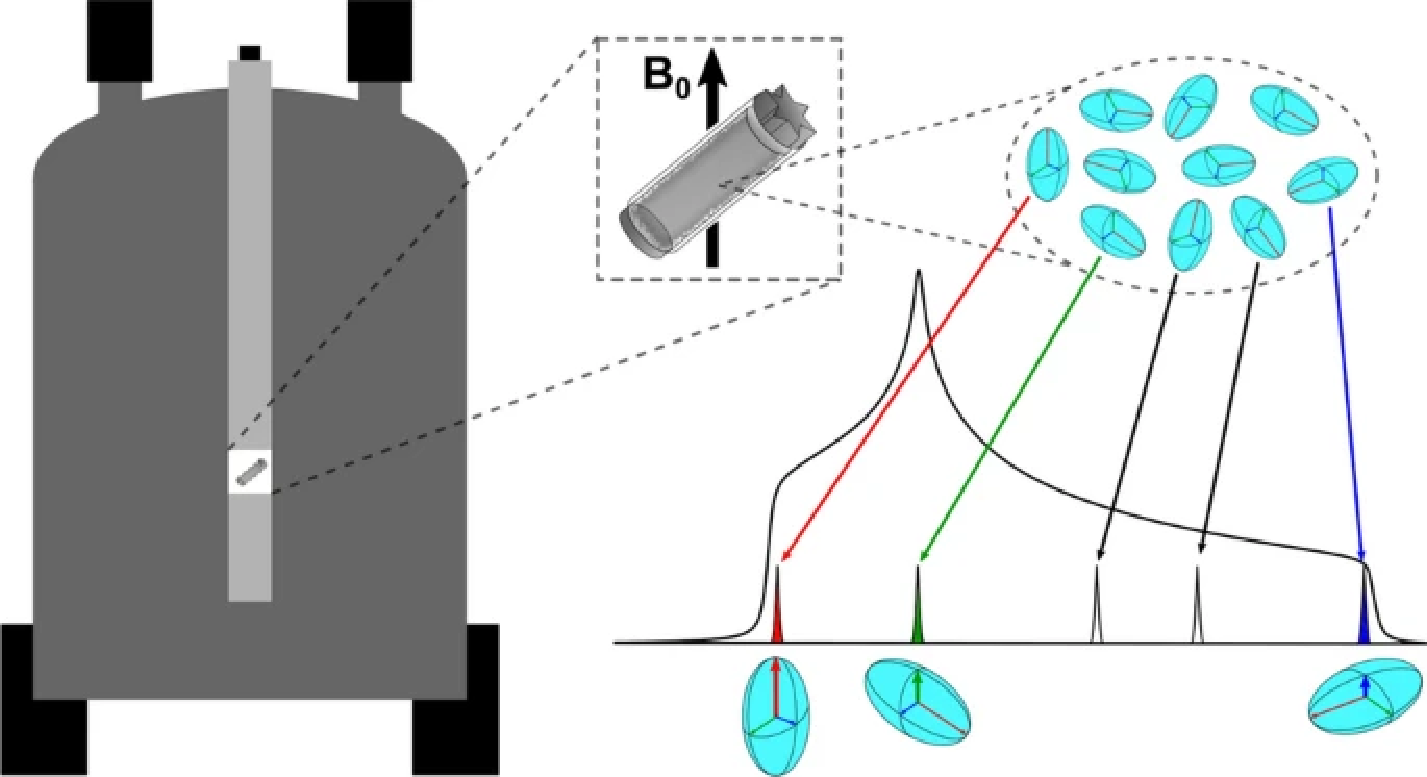
\includegraphics[width=0.45\linewidth]{Figures/ssnmr-tensor.pdf}
  \caption{Characteristic solid-state NMR powder lineshape for an asymmetric tensor e.g. in an alkene. The positions of the three principal values are shown.}
  \label{fig:ssnmr-tensor}
\end{figure}

The extremely poor S/N ratio (especially for a relatively insensitive nucleus like \ce{^{77}Se}) limits the utility of this method, as the radiated signal from the nuclei is spread out over a large bandwidth.
Spinning at the magic angle can improve the S/N ratio by partially averaging out the chemical shift anisotropy and dipolar relaxation.
Instead of the powder pattern, we instead observe a sharp isotropic chemical shift and a series of spinning sidebands which are separated from the isotropic peak by multiples of the spinning frequency.
The radiated power is thus concentrated in narrower bands, leading to a much improved S/N ratio.

An example is presented in \cref{fig:31P-ssnmr} of proton decoupled solid state \ce{^{31}P} spectra of barium diethyl phosphate, reproduced from the work of Herzfeld and Berger\autocite{Herzfeld1980SidebandAngle}.
In the first spectrum, no magic angle spinning was used, and the lineshape is characteristically broadened into an asymmetric peak (the powder lineshape).
Note the poor S/N ratio due to the broad peak.
The S/N ratio can be seen to improve as the spinning speed increases, and the sidebands become more sparse, affording a stronger signal overall.

\begin{figure}
    \centering
    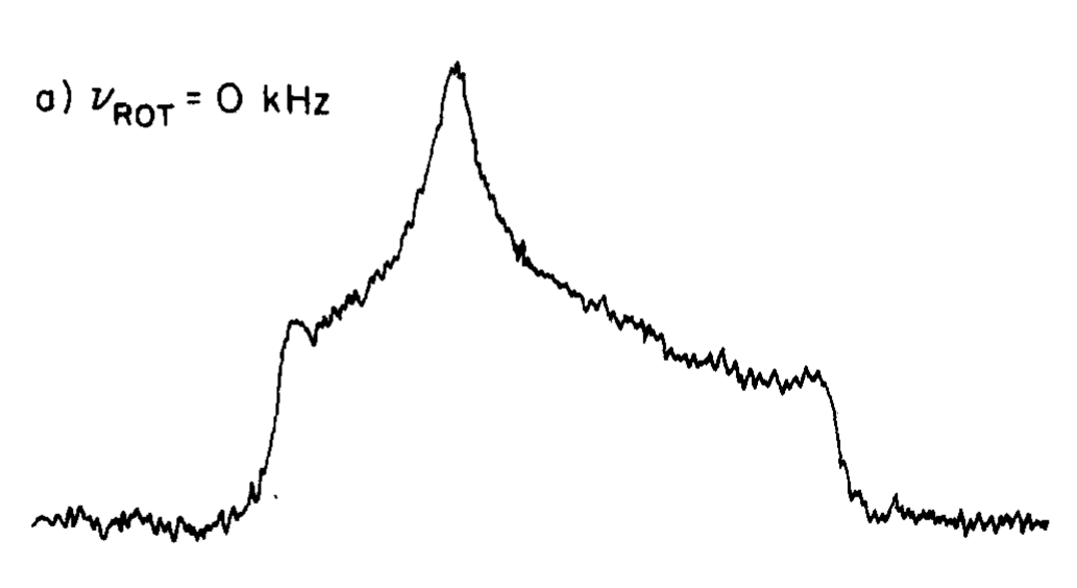
\includegraphics[width=0.45\linewidth]{Figures/31P-ssnmr-0khz.pdf}
    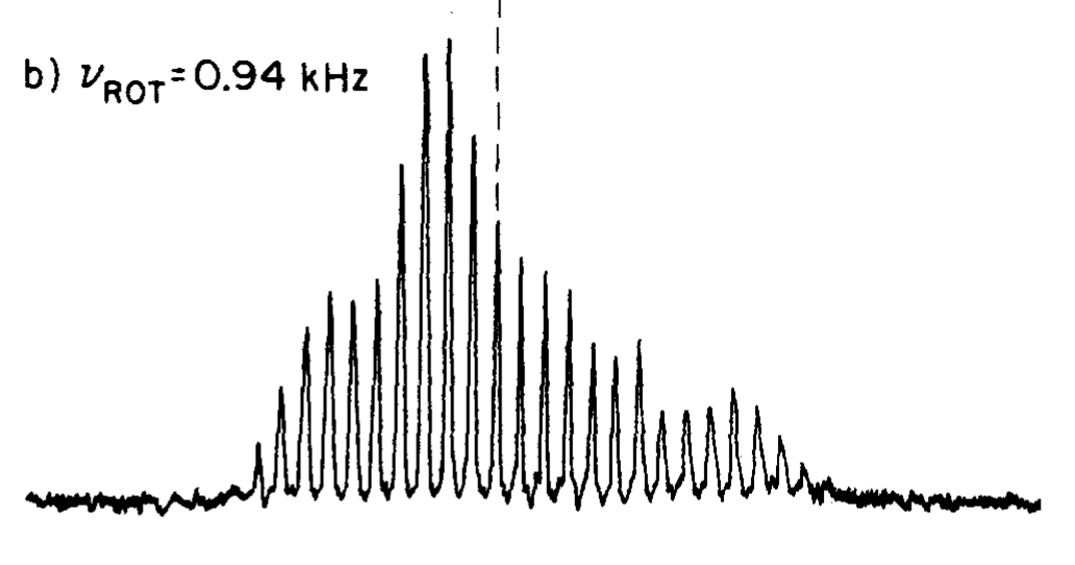
\includegraphics[width=0.45\linewidth]{Figures/31P-ssnmr-0.94khz.pdf}
    
    \includegraphics[width=0.45\linewidth]{Figures/31P-ssnmr-2.06khz.pdf}
    \includegraphics[width=0.45\linewidth]{Figures/31P-ssnmr-2.92khz.pdf}
    \caption{Proton decoupled solid state \ce{^{31}P} spectra of barium diethyl phosphate spinning at the magic angle, at the speed specified. The isotropic chemical shift is shown by the vertical dotted line.}
    \label{fig:31P-ssnmr}
\end{figure}

The principal values of the tensor are clearly easily obtained from a non-spinning sample, as they can practically be read off the spectrum.
However, the extremely poor S/N ratio (especially for a relatively insensitive nucleus like \ce{^{77}Se}) limits the utility of this method.
Spinning at the magic angle is clearly necessary to improve the S/N ratio, however this obscures the true locations of the extrema of the signal, therefore the values of $\delta_{11}$ and $\delta_{33}$, as well as modifying the position of the maximum ($\delta_{22}$).

There exist programs (such as SOLA, integrated within TopSpin by Bruker BioSpin) which can fit an experimental lineshape or sideband manifold affording the principal values of the tensor, however there is clearly a trade-off between obtaining a good S/N ratio and having enough sidebands within the limits of the signal for a meaningful fit.
Another issue is encountered with preferred orientation of crystallites, as in powder diffraction, which is not modelled in the fitting routine, leading to a poorer fit.
Perhaps the most fundamental issue stems from the fact that the sample is a powder of randomly oriented particles.
This means that the absolute orientation of the tensor with respect to the molecule cannot be determined from this kind of experiment.
Nonetheless, the \emph{shape} of the tensor is still valuable information that may be able to shed light on Ch-bonding in the solid phase.

To this end, we acquired solid state spectra of three complexes spanning the range of electron demand, \cmpd{ebs.4ome}$\cdot$DMAP, \cmpd{ebs.ph}$\cdot$DMAP, and \cmpd{ebs.4no2}$\cdot$DMAP.
\footnote{\cmpd{ebs.4ome}$\cdot$DMAP differs from the other structures, in that it crystallises in the space group $P2_1/c$, whereas \cmpd{ebs.ph}$\cdot$DMAP and \cmpd{ebs.4no2}$\cdot$DMAP both crystallise in $P\bar{1}$.
The $2_1$ screw axis in the former crystal is oriented such that it generates a symmetry equivalent molecule which is rotated by an angle of about 45\degree.
This means that the observed chemical shift tensor is the average of these two symmetry related orientations, further complicating the analysis.
Fundamentally this is due to the fact that an ellipsoid does not have twofold rotational symmetry, except about its principal axes.
The triclinic complexes \cmpd{ebs.ph}$\cdot$DMAP and \cmpd{ebs.4no2}$\cdot$DMAP do not suffer from this issue, as the inversion symmetry operation preserves the shape of the tensor.
This can be seen in the latter two principal values of the chemical shift tensor in \cref{tab:77se-ssnmr-ebs-csa}, which have the same value (within experimental error), describing a cigar-shaped tensor.}
The resulting spectra are presented in \cref{fig:77se-ssnmr-ebs}, and the extracted principal values of the chemical shift tensor are presented in \cref{tab:77se-ssnmr-ebs-csa}.

\begin{figure}
  \centering
  \begin{subfigure}{\linewidth}
    \centering
    \includegraphics[height=0.28\textheight]{Figures/ebs-4ome-dmap-cpmas-77se.pdf}
    \caption{\ce{^{77}Se} CPMAS NMR spectrum of \refcmpd{ebs.4ome}$\cdot$DMAP.}
  \end{subfigure}
  \begin{subfigure}{\linewidth}
    \centering
    \includegraphics[height=0.28\textheight]{Figures/ebs-ph-dmap-cpmas-77se.pdf}
    \caption{\ce{^{77}Se} CPMAS NMR spectrum of \refcmpd{ebs.ph}$\cdot$DMAP.}
  \end{subfigure}
  \begin{subfigure}{\linewidth}
    \centering
    \includegraphics[height=0.28\textheight]{Figures/ebs-4no2-dmap-cpmas-77se.pdf}
    \caption{\ce{^{77}Se} CPMAS NMR spectrum of \refcmpd{ebs.4no2}$\cdot$DMAP.}
  \end{subfigure}
  \caption{}
  \label{fig:77se-ssnmr-ebs}
\end{figure}

\begin{table}
  \caption{Principal values of the chemical shift tensor extracted from powder spectra in \cref{fig:77se-ssnmr-ebs}.}
  \begin{tabular}{lllll}
    \toprule
    Complex                                    & $\delta_{\textrm{iso}}$ & $\delta_{11}$  & $\delta_{22}$  & $\delta_{33}$   \\\midrule
   \cmpd{ebs.4ome}$\cdot$DMAP\tablefootnote{Site a}   & 835.2                   & 1572.58        & 466.52         & 466.50          \\
   \cmpd{ebs.4ome}$\cdot$DMAP\tablefootnote{Site b}   & 866.9                   & 1628.91        & 485.95         & 485.92          \\
   \cmpd{ebs.ph}$\cdot$DMAP                           & 864.5                   & 1616.74        & 596.21         & 380.64          \\
   \cmpd{ebs.4no2}$\cdot$DMAP                         & 860.8                   & 1596.92        & 547.82         & 437.66          \\\bottomrule
  \end{tabular}
  \label{tab:77se-ssnmr-ebs-csa}
\end{table}
  

\subsection{Calculation of chemical shift anisotropy}
In order to verify our results, we also \emph{calculated} the chemical shielding tensors in order to compare the principal values, and also determine the likely orientation of the tensors with respect to the rest of the molecule (\cref{fig:77se-tensor-ebs-dmap}).
These calculations were conducted at the $\omega$B97X-D/def2tzvp level, using the GIAO method of calculating shielding tensors.\autocite{Schreckenbach1995CalculationTheory,Schreckenbach1996TheApproximation}
In order to convert these chemical shielding tensors $\sigma$ into chemical shifts $\delta$, we must reference them to a standard $\sigma_{\textrm{ref}}$.
\begin{equation}
  \delta = \sigma_{\textrm{ref}} - \sigma_{\textrm{sample}}
  \label{eqn:shieldingtoshift}
\end{equation}
Convention dictates that for \ce{^{77}Se}, dimethylselenide is assigned a chemical shift of 0~ppm.
The structure of dimethylselenide was therefore optimised and shielding tensors calculated at the same level.

The tensors (in the computation reference frame) were found to be
\begin{align*}    
  \sigma_{\textrm{\ce{Me2Se}}} = &\begin{bmatrix} 2276.3834 & -0.0073 & -0.0175 \\ -0.0159 & 1579.1094 & 0.0349 \\ -0.0622 & -0.0041 & 1583.4669 \end{bmatrix}\\
  \sigma_{\textrm{\cmpd{ebs.ph}}} = &\begin{bmatrix} 1086.4346 & 929.1822 & 929.1822 \\ 862.9168 & 514.6826 & -87.328 \\ 105.4202 & -92.4104 & 1101.0194 \end{bmatrix}\\
  \sigma_{\textrm{\cmpd{ebs.4ome}}\cdot\textrm{DMAP}} = &\begin{bmatrix} 1686.2267 & 105.2547 & -3.2274 \\ 31.1129 & 187.9487 & 48.4737 \\ -19.1247 & 50.3984 & 1081.5651 \end{bmatrix}\\
  \sigma_{\textrm{\cmpd{ebs.ph}}\cdot\textrm{DMAP}} = &\begin{bmatrix} 1595.7999 & 367.4957 & 6.7322 \\ 322.6389 & 291.3611 & 10.8588 \\ -19.9165 & -35.8017 & 1069.2648 \end{bmatrix}\\
  \sigma_{\textrm{\cmpd{ebs.4no2}}\cdot\textrm{DMAP}} = &\begin{bmatrix} 1671.4068 & -76.2797 & 20.6203 \\ -100.0242 & 221.8577 & -17.9295 \\ -44.1025 & -120.0346 & 1055.0806 \end{bmatrix}\\
  \sigma_{\textrm{\cmpd{ebs.ph}}\cdot\textrm{DMF}} = &\begin{bmatrix} 1642.3856 & -138.5717 & -175.547 \\ -111.063 & 175.617 & -253.364 \\ -215.991 & -275.178 & 1028.493 \end{bmatrix}
\end{align*}

affording reference frame independent principal values in \cref{tab:77se-calc-ebs-shielding-csa}.

\begin{table}
  \caption{Principal values of the chemical shielding tensor calculated from optimised structures.}
  \begin{tabular}{lllll}
    \toprule
    Complex                                           & $\sigma_{\textrm{iso}}$ & $\sigma_{11}$  & $\sigma_{22}$  & $\sigma_{33}$   \\\midrule
    \ce{Me2Se}                                        & 1812.9866           & 1579.1093& 1583.4670 & 2276.3834  \\
    \cmpd{ebs.ph}                                     & 900.7122            & -156.9566& 1114.4138 & 1744.6794  \\
    \cmpd{ebs.4ome}$\cdot$DMAP                        & 985.2468            & 182.0846 & 1084.2014 & 1689.4545  \\
    \cmpd{ebs.ph}$\cdot$DMAP                          & 985.4753            & 205.5761 & 1069.2485 & 1681.6013  \\
    \cmpd{ebs.4no2}$\cdot$DMAP                        & 982.7817            & 210.7844 & 1060.7206 & 1676.8400  \\
    \cmpd{ebs.ph}$\cdot$DMF                           & 948.8319            & 80.7668  & 1064.7403 & 1700.9887  \\
    \bottomrule
  \end{tabular}
  \label{tab:77se-calc-ebs-shielding-csa}
\end{table}

These were converted to chemical shifts using \cref{eqn:shieldingtoshift}, which are presented in \cref{tab:77se-calc-ebs-shift-csa}.

\begin{table}
  \caption{Principal values of the chemical shift tensor calculated from optimised structures.}
  \begin{tabular}{lllll}
    \toprule
    Complex                                           & $\delta_{\textrm{iso}}$ & $\delta_{11}$  & $\delta_{22}$  & $\delta_{33}$   \\\midrule
    \cmpd{ebs.ph}                                     & 912.2744            & 1969.9432& 698.5728  & 68.3072    \\
    \cmpd{ebs.4ome}$\cdot$DMAP                        & 827.7398            & 1630.9020& 728.7852  & 123.5321   \\
    \cmpd{ebs.ph}$\cdot$DMAP                          & 827.5113            & 1607.4105& 743.7381  & 131.3853   \\
    \cmpd{ebs.4no2}$\cdot$DMAP                        & 830.2049            & 1602.2022& 752.2660  & 136.1466   \\
    \cmpd{ebs.ph}$\cdot$DMF                           & 864.1547            & 1732.2198& 748.2463  & 111.9979   \\ \bottomrule
  \end{tabular}
  \label{tab:77se-calc-ebs-shift-csa}
\end{table}

These values are encouragingly close to those derived from the fitting of the experimental MAS line shape, with the exception of \cmpd{ebs.4ome}$\cdot$DMAP, for reasons explained above.

Plotting the resulting tensors as ellipsoids reveals aspects of the electron density and hence shielding around the selenium (\cref{fig:77se-tensor-ebs-dmap}).
A major contributor to the tensor is of course the aromatic ring current, which leads to deshielding perpendicular to the plane of the ring.
There is also a ring current in the pyridine ring, which deshields the selenium roughly in the direction of the \ce{Se-C} bond (perpendicular to the plane of the pyridine ring).
This accounts for the large $\delta_{11}$ and $\delta_{22}$ components of the chemical shift.
The remainder is presumably due to diamagnetic shielding from the electron density.
In this we are able to see deformation of the electron cloud due to the lone pairs and the Ch-bond.
The  $\delta_{33}$ component is substantially smaller than $\delta_{11}$ and $\delta_{22}$, and is aligned with the Ch-bond, reflecting a very strong shielding in this direction.
This clearly shows the contribution of the lone pair of the pyridyl nitrogen to the electron density around the selenium, and hence the strength of the Ch-bond.

\begin{figure}
  \centering
  \begin{subfigure}{0.3\linewidth}
    \centering
    \includegraphics[height=3.5cm]{Figures/77se-tensor-ebs-dmap.png}
    \caption{Calculated chemical shift tensor for \refcmpd{ebs.ph}$\cdot$DMAP.}
    \label{fig:77se-tensor-ebs-dmap}
  \end{subfigure}
  \begin{subfigure}{0.3\linewidth}
    \centering
    \includegraphics[height=3.5cm]{Figures/77se-tensor-ebs-dmf.png}
    \caption{Calculated chemical shift tensor for \refcmpd{ebs.ph}$\cdot$DMF.}
    \label{fig:77se-tensor-ebs-dmf}
  \end{subfigure}
  \begin{subfigure}{0.3\linewidth}
    \centering
    \includegraphics[height=3.5cm]{Figures/77se-tensor-ebs.png}
    \caption{Calculated chemical shift tensor for \refcmpd{ebs.ph}.}
    \label{fig:77se-tensor-ebs}
  \end{subfigure}
\end{figure}

This can be contrasted to the chemical shift of the non-complexed selenium (\cref{fig:77se-tensor-ebs}).
In the absence of the lone pair of the pyridyl nitrogen, the $\sigma$-hole strongly deshields the selenium, therefore the large $\delta_{11}$ component is roughly aligned with it. 
There is also no deshielding ring current from the pyridine, so the $\delta_{33}$ (which is aligned with the \ce{Se-C} bond) is very small.
The $\delta_{22}$ component perpendicular to the plane of the benzisoselenazolinone ring is roughly the same, as there is no significant change in either electron density or ring currents in this direction.

To demonstrate that the $\delta_{11}$ component in the \cmpd{ebs.ph}$\cdot$DMAP complex is not entirely due to the pyridine ring current, a \cmpd{ebs.ph}$\cdot$DMF complex was optimised and the chemical shift tensor calculated.
This is shown in \cref{fig:77se-tensor-ebs-dmf}.
The largest component of the tensor is still approximately aligned with the \ce{Se-C} bond, even in the absence of the aromatic base.

These results must be taken with a grain of salt, as the chemical shifts are calculated in the gas phase (i.e. in the absence of crystal packing).
This is particularly important for the chemical shift of the non-complexed heterocycle, as such a ``free'' $\sigma$-hole would not be observed in any condensed phase (it is always filled by solvent in solution, or the carbonyl of an adjacent molecule in the solid).
Nonetheless we may draw comparisons with this caveat in mind.

\subsubsection{Measurement of CSA in a single crystal}
The calculated chemical shift tensors were useful in the absence of experimental data, and the fact that the principal values of the tensors matched the powder data so well was encouraging.
However, we wished to verify the orientation of the tensor by an experimental method.

We were fortunate to obtain a single crystal of \cmpd{ebs.ph}$\cdot$DMAP of sufficient size (approx $10\times3\times1$~mm, \cref{fig:ebs-ph-dmap-picture}) for a single crystal SS-NMR experiment, allowing us to measure the orientation of the tensor in that crystal for comparison with our computational results.\footnote{Unfortunately no other derivatives formed crystals of sufficient size or morphology for the SS-NMR experiment.}

\begin{figure}
  \centering
  \includegraphics[width=0.4\linewidth]{Figures/ebs-ph-dmap-picture.jpg}
  \caption{Single crystal of \cmpd{ebs.ph}$\cdot$DMAP used for SS-NMR.}
  \label{fig:ebs-ph-dmap-picture}
\end{figure}

In order to do this, the faces of the crystal had to be indexed to the internal structure, which was done by x-ray diffraction.
As the crystal was far too big to mount on the diffractometer, two faces were marked with different coloured pens to preserve the relation to the large crystal, then a small fragment was removed from the crystal.
This was mounted, and a short data collection afforded an indexable pattern.
The resulting planes are shown in \cref{fig:ebs-ph-dmap-index}.

\begin{comment}
\begin{figure}
  \centering
  \includegraphics[width=0.4\linewidth]{Figures/xtal-b.jpg}
  \includegraphics[width=0.4\linewidth]{Figures/xtal-c.jpg}
  \caption{Indexed faces of \cmpd{ebs.ph}$\cdot$DMAP.}
  \label{fig:ebs-ph-dmap-index}
\end{figure}
\end{comment}


\begin{figure}
  \centering
  \includegraphics[width=0.7\linewidth]{Figures/indices.png}
  \caption{Internal structure of crystal with indexed faces. The plane normal to the Ch-bond is indicated in yellow.}
  \label{fig:ebs-ph-dmap-index}
\end{figure}

The large crystal was then mounted in a goniometer probe, and spectra were acquired on a 600~MHz instrument using a Hahn echo pulse sequence.
This was necessary to preseve the extremely weak signal by isolating it from the excitation pulse in the time domain.
The spectra were referenced to a saturated solution of diphenyldiselenide in \ce{CDCl3} at 463~ppm, which was contained in a zirconia MAS rotor.\autocite{Duddeck1995}

The crystal orientation with respect to the magnetic field is depicted in \cref{fig:ebs-ph-dmap-magfield-index}, and the resulting spectrum is shown in \cref{fig:ebs-dmap-hahnecho-77se}.
The selenium nucleus in this orientation resonates at 437~ppm.

\begin{figure}
  \centering
  \includegraphics[width=0.3\linewidth]{Figures/ebs-ph-dmap-magfield-index.pdf}
  \caption{Orientation of the magnetic field with respect to the crystal. $B_{0}$ is aligned with the $(0 0 1)$ crystal direction.}
  \label{fig:ebs-ph-dmap-magfield-index}
\end{figure}

\begin{figure}
  \centering
  \includegraphics[width=0.8\linewidth]{Figures/ebs-dmap-hahnecho-77se.pdf}
  \caption{\ce{^{77}Se} NMR spectrum of a single crystal of \refcmpd{ebs.ph}$\cdot$DMAP in the orientation depicted in \cref{fig:ebs-ph-dmap-magfield-index}.}
  \label{fig:ebs-dmap-hahnecho-77se}
\end{figure}

Using the relationship in \cref{eqn:orientation-csa}, we are able to derive the polar angles which relate the principal axis system of the chemical shift tensor to the laboratory coordinate system.
In this case, as can be seen in \cref{fig:ebs-ph-dmap-magfield-index}, the laboratory reference frame (or at least the $z$-axis) is coincicent with the $c$-axis of the crystal, which greatly simplifies analysis by obviating the need for a further transformation between the crystal axes and laboratory reference.

DO THIS

We can calculate the chemical shift tensor using the diagonal components from the powder experiment and the rotation matrix from the polar angles:
\begin{equation}\resizebox{.9\hsize}{!}{$
  \delta = \begin{bmatrix} \cos\theta & \sin\theta\sin\phi & \sin\theta\cos\phi \\ 0 & \cos\phi & -\sin\phi \\ -\sin\theta & \cos\theta\sin\phi & \cos\theta\cos\phi \end{bmatrix}
  \begin{bmatrix} 1616.74 & 0 & 0 \\ 0 & 596.21 & 0 \\ 0 & 0 & 380.64 \end{bmatrix}
  \begin{bmatrix} \cos\theta & \sin\theta\sin\phi & \sin\theta\cos\phi \\ 0 & \cos\phi & -\sin\phi \\ -\sin\theta & \cos\theta\sin\phi & \cos\theta\cos\phi \end{bmatrix}^{-1}$}
\end{equation}
which affords
\begin{equation}
  \delta = \begin{bmatrix} 0 & 0 & 0 \\ 0 & 0 & 0 \\ 0 & 0 & 0 \end{bmatrix}
\end{equation}
and hence\begin{equation}
  \sigma = \begin{bmatrix} 0 & 0 & 0 \\ 0 & 0 & 0 \\ 0 & 0 & 0 \end{bmatrix}
\end{equation}

This agrees very well with the calculated tensor, and strongly supports our assertion that the chemical shift anisotropy is influenced by the $\sigma$-hole.

To briefly summarise, Ch-bonding induces enormous chemical shift anisotropy at the selenium, which is highly sensitive to the approach of the Lewis base and can be measured using both powder and single crystal SSNMR.
While the technique is perhaps not as sensitive as diffraction based methods, the great advantage lies in the fact that SSNMR does not require crystallinity, even at the nano scale.
This means that amorphous species such as polymers may be studies, as long as they contain an NMR active nucleus.

\subsection{Solution-phase studies}
While the above crystallographic analysis gives a useful qualitative understanding of the strength of the Ch-bond, we sought an experimental method that could accurately determine bond energies, so that we could easily compare our Ch-bonded complexes with those dominated by other interactions.

\subsubsection{NMR titration experiments}
NMR titrations are a useful tool for the determination of binding affinities in supramolecular and host-guest chemistry.
\ce{^{1}H} and \ce{^{19}F} NMR have both been used to study halogen bonded systems, however we decided to take advantage of the unique NMR characteristics of the \ce{^{77}Se} nucleus to probe the Ch-bond in our systems for the following reasons:

\begin{itemize}
    \item the nucleus has an extremely wide chemical shift range (-1000--2000~ppm),
    \item the chemical shift is very sensitive to the electronic environment around the selenium,
    \item the selenium is at the heart of the interaction, so any electronic changes should manifest clearly,
    \item the spectrum (for our compounds) is extremely simple, featuring only one singlet,
    \item the experiment is moderately sensitive (slightly more sensitive than \ce{^{13}C}).
\end{itemize}

We devised a titration experiment, where a solution of a Lewis base is gradually added to a solution of the Ch-bond donor, and the chemical shift of the selenium is measured at the various concentrations of base.
As the concentration of base increases, a greater proportion of the selenium species will be in a Ch-bonded environment, with an associated increase in electron density at the selenium due to the coordinated base.
This will lead to an upfield shift of the selenium resonance.

It is important to note that even in the absence of a Lewis base, the organoselenium species will still likely feature a Ch-bond to the carbonyl oxygen of another molecule.
This interaction can be seen to dominate the crystal packing of ebselen derivatives in the absence of any other coordinating species.
This is substantially weaker than a \ce{Se\dots N} interaction, but non-negligible.
We must therefore view these as \emph{competition} experiments, rather than an absolute measure of binding energy.

For single site binding (a valid approximation for these systems, as the single $\sigma$-hole is likely to out-compete all other interactions), the dissociation constant can be expressed as

\begin{equation}
    \label{eqn:equilibrium}
    \mathrm{K_d} = \frac{[\mathrm{ebs}][\mathrm{base}]}{[\mathrm{ebs\cdot base}]}
\end{equation}

If the Ch-bond formation/breaking is slow on the NMR timescale, two distinct resonances will be observed that correspond to the ``free'' (Ch-bonded to a carbonyl oxygen) and ``bound'' (Ch-bonded to the Lewis base) selenium species, and their relative concentrations can be determined by integration of the signals.
As it happens, this is not the case, and the process is fast relative to the NMR timescale.
The observed chemical shift is therefore the mole fraction ($f_\mathrm{ebs} = [\mathrm{ebs}]/[\mathrm{ebs}]_0$ and $f_\mathrm{ebs\cdot base} = [\mathrm{ebs\cdot base}]/[\mathrm{ebs}]_0$) weighted average of the chemical shifts of the two species:
\begin{equation}
    \delta_{\mathrm{observed}} = \delta_{\mathrm{ebs}} f_\mathrm{ebs} + \delta_{\mathrm{ebs\cdot base}} f_{\mathrm{ebs\cdot base}}
\end{equation}

If we consider only the \emph{change} in chemical shift from the free species, this becomes simply:
\begin{align}
    \Delta(\delta_{\mathrm{observed}}) & = \Delta(\delta_{\mathrm{ebs\cdot base}}) f_{\mathrm{ebs\cdot base}} \\
    & = \Delta(\delta_{\mathrm{ebs\cdot base}}) \left(\frac{[\mathrm{ebs\cdot base}]}{[\mathrm{ebs}]_0}\right)
\end{align}

From here we can rearrange the equilibrium expression (\cref{eqn:equilibrium}) and mass balance equation ($[\mathrm{ebs}]_0 = [\mathrm{ebs}] + [\mathrm{ebs\cdot base}]$), and substitute them in to arrive at the generic binding isotherm equation:
\begin{equation}
    \Delta(\delta) = \frac{\Delta(\delta_{\mathrm{ebs\cdot base}})  \times [\mathrm{base}]}{\mathrm{K_{d}} + [\mathrm{base}]}
\end{equation}

This assumes that there is insignificant depletion of the base concentration due to complexation.\autocite{Thordarson2011}
Such an assumption may not be entirely valid for this situation, which may explain the imperfect fitting.
However, the analysis is considerably simplified, and adequate standard deviations are obtained using this method.

The resulting K\textsubscript{d} values can be converted to free energies:
\begin{equation}
    \Delta G = -RT \ln{\mathrm{K_d}}
\end{equation}

A saturated solution of the organoselenium derivative in chloroform was used, due to the high solubility (to reduce acquisition time) and non-coordinating nature (to minimise Ch-bonding to the solvent).
This was spiked with a small amount of deuterochloroform for the lock signal.
Spectra were acquired on a 500~MHz instrument, using a 60\degree~pulse and 1~s relaxation delay, until an unambiguous \ce{^{77}Se} resonance was observed.
The resulting chemical shifts were then tabulated and plotted against the concentration of the Lewis base.
These are shown in \cref{fig:nmr-titrations}.

\begin{figure}
    \centering
    \includegraphics[width=0.45\linewidth]{Figures/nmr-titration/bn-ebs-dmap.eps}
    \includegraphics[width=0.45\linewidth]{Figures/nmr-titration/4oet-ebs-dmap.eps}
    
    \includegraphics[width=0.45\linewidth]{Figures/nmr-titration/ebs-dmap.eps}
    \includegraphics[width=0.45\linewidth]{Figures/nmr-titration/4br-ebs-dmap.eps}
    
    \includegraphics[width=0.45\linewidth]{Figures/nmr-titration/4cn-ebs-dmap.eps}
    \caption[NMR titration binding isotherms]{Binding isotherms for ebselen derivatives \refcmpd{ebs.bn,ebs.4oet,ebs.ph,ebs.4br,ebs.4cn} with DMAP. Scatchard plots are inset.}
    \label{fig:nmr-titrations}
\end{figure}

Non-linear regression analysis was performed with the \texttt{nls} function in the R software package using the relationship derived above, and the calculated values are given in \cref{tab:nmr-titrations}.\autocite{R}

\begin{table}
    \centering
    \begin{tabular}{lll}\toprule
        Complex & Binding energy (kcal/mol) & $\Delta(\delta_{\mathrm{ebs\cdot base}})$ (ppm) \\\midrule
        \cmpd{ebs.bn}$\cdot$DMAP & 0.17(6) & 41.6 \\
        \cmpd{ebs.4oet}$\cdot$DMAP & 0.47(3) & 102.8 \\
        \cmpd{ebs.4br}$\cdot$DMAP & 0.87(5) & 104.2 \\
        \cmpd{ebs.ph}$\cdot$DMAP & 1.12(4) & 70.05 \\
        \cmpd{ebs.4cn}$\cdot$DMAP & 2.28(5) & 82.62 \\\bottomrule
    \end{tabular}
    \caption[NMR titration binding energies]{Binding energies for complexes of \refcmpd{ebs.bn,ebs.4oet,ebs.4br,ebs.ph,ebs.4cn} with DMAP, derived from \ce{^{77}Se}-NMR titration experiments.}
    \label{tab:nmr-titrations}
\end{table}

Although there is insufficient data to derive clear trends from a Hammett relationship, we can nevertheless visualise the data in a plot, which shows that the Ch-bond gets appreciably stronger with more electron withdrawing substituents (\cref{fig:hammett-dmap-nmr}).

\begin{figure}
    \centering
    \includegraphics[width=0.75\linewidth]{Figures/hammett-dmap-nmr.eps}
    \caption{Hammett plot of binding energies between ebselen derivatives and DMAP, determined by \ce{^{77}Se}-NMR titration. The line is described by the equation $\Delta\mathrm{G} = (0.88(21) + 1.86(57) \times \sigma_{\mathrm{X}})$~kcal$\cdot$mol$^{-1}$ ($\mathrm{R}^2 = 0.8437$).}
    \label{fig:hammett-dmap-nmr}
\end{figure}


\subsubsection{UV-Vis titration experiment}
Although extremely useful, the NMR titration technique had a number of drawbacks.
Firstly, relatively large amounts ($\sim$100~mg) of the Ch-bond donor were required.
For simple systems such as these, this was not an issue, however we hoped to apply the technique to less synthetically accessible molecules, which may not be available in such quantities.
Secondly, the experiment is quite time consuming, with tens of minutes required per spectrum.

UV-Vis spectroscopy presented a possible solution to both of these issues, with spectra collected in seconds even with extremely dilute solutions.
Interactions which have a charge-transfer component (such as Ch-bonding) can give rise to strong absorbances attributable to the n $\rightarrow \sigma^{\star}$ transition.\autocite{Blackstock1987}
However, we were unable to observe any evidence of such absorbances in our systems.
This may be due to the fact that these Ch-bonds are primarily electrostatic in origin, or because the aromatic systems are already strongly absorbing, thus obscuring the charge-transfer band.

\subsection{Ch-bonding in the gas phase}
To complete our trifecta of experiments, we sought evidence that supports Ch-bonding in the gas phase.
Broadly, we intended to isolate an ion corresponding to the complex by mass spectrometer, and subsequently fragment it by CID to regain the original species.
Naturally, this requires that one (or both) of the components of the complex have a charge, so that it can be detected by the mass spectrometer.
We initally injected an equimolar mixture of DMAP and ebselen \cmpd{ebs.ph} in methanol, and isolated an ion of m/z 398.08 a.m.u.
However, this could be assigned to either the desired Ch-bonded complex, protonated at the carbonyl oxygen, or to a H-bonded complex.
CID of this ion exclusively gave an ion of m/z 123.09 a.m.u., corresponding to protonated DMAP (\cref{fig:pos-esi-ms}).
We interpreted this as evidence that we had formed the H-bonded complex, as migration of the proton on the timescale of a collision is unlikely, and the proton is most likely to remain with the more basic species in the H-bond.
Furthermore, a \ce{N+ -H\cdots O} hydrogen bonds are very strong (in excess of 15~kcal/mol)\autocite{Emsley1980}, which is likely to out compete Ch-bonding, with estimated bond enthalpies of <~10~kcal/mol in the gas phase.

\begin{figure}
    \centering
    \includegraphics[scale=0.8]{Figures/pos-esi-ms.eps}
    \caption[Positive mode ESI of \refcmpd{ebs.ph}$\cdot$DMAP$\cdot$\ce{H+}]{Dissociation of the complex \refcmpd{ebs.ph}$\cdot$DMAP$\cdot$\ce{H+} under CID.}
    \label{fig:pos-esi-ms}
\end{figure}

To circumvent this preferential formation of an H-bonded complex, we devised a system with no possibility of H-bonding.
The isonicotinate ion was used as the Lewis base, and the complex isolated in the negative ion mode with m/z 397.01 a.m.u.
CID of this ion exclusively gave a species of m/z 122.02 a.m.u., corresponding to isonicotinate (\cref{fig:neg-esi-ms}).
This provides strong evidence that a Ch-bonded complex is able to be formed in the gas phase.

\begin{figure}
    \centering
    \includegraphics[scale=0.8]{Figures/neg-esi-ms.eps}
    \caption[Negative mode ESI of \refcmpd{ebs.ph}$\cdot$isonicotinate]{Dissociation of the complex \refcmpd{ebs.ph}$\cdot$isonicotinate under CID.}
    \label{fig:neg-esi-ms}
\end{figure}

Using the technique of CID, one could imagine an experiment where such a Ch-bonded complex is fragmented with gradually increasing energy, and the yield of the product ion measured.
This could theoretically be correlated with the gas phase bond energy.
Indeed, this is the basis of the technique of Threshold CID (TCID) developed by Armentrout.\autocite{Armentrout2003,Rodgers2000,Narancic2007}
Although the experiment is simple, the data analysis is not.
This is due to the often poorly characterised energy distribution of the reactant ions, and vibrational energy redistribution in the products.
These barriers are not insurmountable for simple systems (the technique has been successfully applied to metal complexes, and small non-covalent complexes), but in our moderately complex molecules with many vibrational modes, errors are likely to dominate any values extracted from the experiment.
However, we present here a proof of concept experiment, which shows the decrease in reactant ion intensity and increase in product ion as CID energy is increased (\cref{fig:ebs-tcid}).

\begin{figure}
    \centering
    TODO
    %\includegraphics{Figures/ebs-tcid.pdf}
    \caption[TCID experiment of \refcmpd{ebs.ph}$\cdot$isonicotinate]{Rudimentary TCID experiment of \refcmpd{ebs.ph}$\cdot$isonicotinate.}
    \label{fig:ebs-tcid}
\end{figure}

\section{Supplementary materials}

\subsection{Synthetic procedures}

\subsubsection[Preparation of \refcmpd{diselenide}]{Preparation of bis(2-carboxyphenyl)diselenide \refcmpd{diselenide}}
\label{sec:diselenide_prep}
%TF-7-3
%KNOWN
Anthranilic acid (3.460~g, 25.33~mmol) was dissolved in 1~\textsc{M} hydrochloric acid (80~mL) and cooled to 0\degree C.
Sodium nitrite (1.751~g, 25.37~mmol) in water (40~mL) was then added drop-wise with stirring.
The mixture was kept at 0\degree C.

Selenium (2.080~g, 26.34~mmol) was suspended in 1~\textsc{M} sodium hydroxide (120~mL) and degassed by repeatedly evacuating the flask until the solvent began to boil, then backfilling with \ce{N2}.
One grain of sodium borohydride was added under \ce{N2} counter flow, followed by hydrazine hydrate (1.3~mL, 26~mmol).
The mixture was heated until a red colour appeared, then cooled to 0\degree C.

The diazonium solution was neutralised with a solution of sodium hydroxide (4.320~g, 108.0~mmol) in water (20~mL), then added slowly to the cooled diselenide solution.
Upon completion, the mixture was warmed to room temperature and stirred for 1~h, then neutralised with concentrated hydrochloric acid.
The dense precipitate was separated by centrifuging, the supernatant decanted off, and the residue resuspended in hot methanol (300~mL).
The methanol solution was subjected to hot filtration, and the orange filtrate concentrated to a volume of $\sim$100~mL.
This was cooled to -20\degree C, and the resulting crystals filtered off and dried.
Recrystallisation from methanol gave \cmpd{diselenide} as a pale brown powder (1.8718~g, 37\%).

\ce{^{1}H} NMR (400~MHz, \ce{\emph{d}6}-DMSO) $\delta$ ppm
7.29--7.38 (m, 1 H),
7.47 (t, \emph{J}=7.43~Hz, 1 H),
7.66 (d, \emph{J}=8.22~Hz, 1 H),
8.02 (d, \emph{J}=7.43~Hz, 1 H)
13.70 (br. s., 1 H).

MS (ESI +ve) m/z 424.8806 (\ce{MNa+}) \ce{C14H11O4Se2+} requires 424.8802 ($\Delta$=0.941~ppm).

\subsubsection[Preparation of \refcmpd{dichloride}]{Preparation of 2-(chlorocarbonyl)phenylselenyl chloride \refcmpd{dichloride}}
Diselenide \refcmpd{diselenide} (1.4758~g, 3.6881~mmol) was dissolved in thionyl chloride (10~ml) with 2 drops DMF, and heated to reflux for 90~minutes.
The excess thionyl chloride was distilled off under reduced pressure, and the solid residue extracted into dry hexane (30~mL).
Evaporation of the solvent afforded \cmpd{dichloride} as yellow crystals (1.870~g, 100\%), which were used without further purification or characterisation.

\subsubsection[General procedure for the preparation of benzisoselenazolinone derivatives (procedure A)]{General procedure for the preparation of benzisoselenazolinone derivatives \refcmpd{ebs.ph,ebs.4cn,ebs.4cf3,ebs.4br,ebs.4co2et,ebs.4ome,ebs.4oet} (procedure A)}
The appropriate amine (2.5~mmol) was dissolved in anhydrous acetonitrile (5~mL) and cooled to 0\degree C.
To this was added triethylamine (1~mL, distilled from \ce{CaH2}), followed by \cmpd{dichloride} (2.5~mmol) in a further 5~mL anhydrous acetonitrile.
The mixture was stirred at room temperature for 2~h, then the solvent was removed under vacuum.
The solid residue was triturated with water (5~mL) and 1~\textsc{M} hydrochloric acid to afford a friable solid, which was purified by recrystallisation from ethyl acetate at -20\degree~C to afford the pure benzisoselenazolinone derivative.

\subsubsection[Procedure for the preparation of benzisoselenazolinone derivatives (procedure B)]{Procedure for the preparation of benzisoselenazolinone derivative \refcmpd{ebs.4no2} (procedure B).}
Sodium hydride (60\% suspension in mineral oil, 125.0~mg, 3.125~mmol) was suspended in anhydrous THF (5~mL) and cooled to 0\degree C.
4-Nitroaniline (treated with charcoal and crystallised from aqueous ethanol, 277~mg, 2.01~mmol) was then added and the resulting dark red suspension stirred for 5 minutes at 0\degree C.
DMAP (16.3~mg, 0.133~mmol) was then added, followed by a solution of the dichloride \cmpd{dichloride} (2.00~mmol) in a further 5~mL anhydrous THF.
The mixture was then warmed to room temperature, and stirred for 18~h to give a light yellow suspension, which was quenched with methanol (5~mL), then suspended in water (50~mL).
The resulting solid was filtered off, washed with 1~\textsc{M} \ce{HCl} and water, then dried to give a light yellow powder (336.0~mg, 52\%).


\paragraph{Ebselen \refcmpd{ebs.ph}}
Colourless crystals, m.p. 182.1--182.3\degree C ($\alpha$ polymorph), 173.4-174.6\degree C ($\beta$ and $\gamma$ polymorph), xx\%.

\ce{^{1}H} NMR (499~MHz, \ce{\emph{d}6}-DMSO) $\delta$ ppm 8.07 (1H, d, \emph{J} = 8.02~Hz), 7.90 (1H, d, \emph{J} = 7.45~Hz), 7.68 (1H, t, \emph{J} = 7.25~Hz), 7.61 (2H, d, \emph{J} = 7.68~Hz), 7.52--7.42 (3H, m), 7.26 (1H, t, \emph{J} = 7.39~Hz).

\paragraph{4-Nitro ebselen \refcmpd{ebs.4no2}}
Pale yellow crystals, 52\%.

\ce{^{1}H} NMR (400~MHz, \ce{CDCl3}) $\delta$ ppm 8.30 (2H, d, \emph{J} = 9.07~Hz), 8.14 (1H, d, \emph{J} = 7.82~Hz), 7.92 (2H, d, \emph{J} = 9.07~Hz), 7.75--7.66 (2H, m), 7.52 (1H, t, \emph{J} = 6.8~Hz).

\ce{^{1}H} NMR (499~MHz, \ce{\emph{d}6}-DMSO) $\delta$ ppm 8.30 (2H, d, \emph{J} = 9.15~Hz), 8.18 (1H, d, \emph{J} = 8.08~Hz), 8.05 (2H, d, \emph{J} = 9.16~Hz), 7.94 (1H, d, \emph{J} = 7.72~Hz), 7.71 (1H, t, \emph{J} = 7.02~Hz), 7.5 (1H, t, \emph{J} = 7.45~Hz).

MS (ESI +ve) m/z 400.0005 (\ce{MNa+} + acetone) \ce{C16H14N2NaO4Se+} requires 401.00110 ($\Delta$=1.52~ppm).

\paragraph{4-Cyano ebselen \refcmpd{ebs.4cn}}
%TF-7-1C
Colourless crystals, m.p. 191\degree C (dec.), 61\%.

\ce{^{1}H} NMR (600~MHz, \ce{\emph{d}6}-DMSO) $\delta$ ppm 8.20 (1H, d, \emph{J} = 8.08~Hz), 7.94--7.83 (5H, m), 7.65 (1H, t, \emph{J} = 7.61~Hz), 7.45 (1H, t, \emph{J} = 7.42~Hz).

\ce{^{13}C} NMR (151~MHz, \ce{\emph{d}6}-DMSO) $\delta$ ppm 166.03, 145.18, 139.4, 133.88, 133.81, 133.03, 129.37, 128.47, 126.78, 126.74, 124.28, 119.20, 114.08, 107.18.

\ce{^{77}Se} NMR (95~MHz, \ce{\emph{d}6}-DMSO) $\delta$ ppm 897.93.

\cmpd{ebs.4cn}$\cdot$DMAP m.p. 157.6--160.2\degree C (DCM solvate, P$2_1/c$).

\cmpd{ebs.4cn}$\cdot$DMAP m.p. 176.0--178.8\degree C (non-solvate, P$bca$).

\paragraph{4-Trifluoromethyl ebselen \refcmpd{ebs.4cf3}}
Colourless crystals, m.p. 184.6--186.4\degree C, 14\%.

\ce{^{1}H} NMR (499~MHz, \ce{\emph{d}6}-DMSO) $\delta$ ppm 8.27 (1H, d, \emph{J} = 7.41~Hz), 8.01--7.96 (1H, m), 7.95--7.89 (1H, m), 7.88--7.81 (3H, m), 7.76 (2H, d, \emph{J} = 8.41~Hz).

\cmpd{ebs.4cf3}$\cdot$DMAP m.p. 178.3--179.6\degree C.

\paragraph{4-Bromo ebselen \refcmpd{ebs.4br}}
Colourless crystals, m.p. 189.7--190.7\degree C,, 18\%.

\cmpd{ebs.4br}$\cdot$DMAP m.p. 162.3--164.4\degree C.

\paragraph{4-Carboxyethyl ebselen \refcmpd{ebs.4co2et}}
Colourless crystals, m.p. 173.1--174.5\degree C 13\%.

\ce{^1H} NMR (500~MHz, DMSO-\emph{d6}) $\delta$ 8.08 (d, \emph{J} = 7.8~Hz, 1H), 8.02 (d, \emph{J} = 8.7~Hz, 2H), 7.92 (dd, \emph{J} = 0.4, 8.0~Hz, 1H), 7.88 (d, \emph{J} = 8.6~Hz, 2H), 7.71 (t, \emph{J} = 7.0~Hz, 1H), 7.50 (t, \emph{J} = 7.3~Hz, 1H), 4.32 (q, \emph{J} = 7.2~Hz, 2H), 1.33 (t, \emph{J} = 7.1~Hz, 3H). 

\cmpd{ebs.4co2et}$\cdot$DMAP m.p. 136.0-138.7\degree C.

\paragraph{4-Methyl ebselen \refcmpd{ebs.4me}}
Light brown crystals, 58\%.

\ce{^1H} NMR (400~MHz, DMSO-\emph{d6}) $\delta$ 8.06 (d, J = 8.0 Hz, 1H), 7.87 (d, J = 7.3 Hz, 1H), 7.66 (dt, J = 0.3, 7.4 Hz, 1H), 7.48 (d, J = 8.3 Hz, 2H), 7.46 (t, J = 7.3 Hz, 1H), 7.24 (d, J = 8.2 Hz, 2H), 2.31 (s, 3H). 

\paragraph{4-Methoxy ebselen \refcmpd{ebs.4ome}}
Light brown crystals, 67\%.

\ce{^1H} NMR (500~MHz, DMSO-\emph{d6}) $\delta$ 8.07 (d, J = 7.9 Hz, 1H), 7.88 (d, J = 7.6 Hz, 1H), 7.67 (t, J = 7.1 Hz, 1H), 7.49 (d, J = 8.4 Hz, 2H), 7.47 (t, J = 6.9 Hz, 1H), 7.01 (d, J = 8.6 Hz, 2H), 3.78 (s, 3H). 

\paragraph{4-Ethoxy ebselen \refcmpd{ebs.4oet}}
Light brown crystals, 67\%.

\ce{^1H} NMR (500~MHz, DMSO-\emph{d6}) $\delta$ 8.06 (d, J = 8.0 Hz, 1H), 7.87 (d, J = 7.5 Hz, 1H), 7.67 (t, J = 7.2 Hz, 1H), 7.48 (t, J = 3.2 Hz, 1H), 7.47 (d, J = 8.8 Hz, 2H), 6.99 (d, J = 8.8 Hz, 2H), 4.05 (q, J = 7.0 Hz, 2H), 1.34 (t, J = 6.9 Hz, 3H). 

\normalsize

\subsection{Crystallisation methods}
Crystals of sufficient quality for x-ray diffraction analysis were grown by vapour diffusion of pentane into a dichloromethane solution ($\sim$50~mg/mL) of either the pure Ch-bond donor, or a 1:1 mixture of the donor and the appropriate Lewis base, with the following exceptions:
\begin{itemize}
    \item the non-solvate of \cmpd{ebs.4cn}$\cdot$DMAP was grown by slow evaporation from THF,
    \item second polymorphs of \cmpd{ebs.4oet}$\cdot$DMAP and \cmpd{ebs.4ome}$\cdot$DMAP were grown from diffusion of pentane into diethyl ether.
\end{itemize}

\subsection{Crystallographic data}



\printbibliography[heading=subbibliography]
\end{refsection}

%\part{Chalcogen bonding at oxygen}
\begin{refsection}

\chapter{Experimental evidence of Chalcogen bonding at oxygen.}

This chapter was published in Chem. Commun., 13 Feb 2020\autocite{Fellowes2020}. \footnote{Compound numbering, section titles, and terminology have been updated to fit this thesis.}
Further experiments are detailed in \cref{app:o-ch-bonding}.

\section{Abstract}
An \emph{o}-nitro-O-aryl oxime was observed to exhibit a short O$\cdots$O contact, which exhibited characteristics consistent with a chalcogen bond.
The \ce{O-N} bond length of the oxime was appreciably longer than the expected value, and
NBO calculations indicated the presence of a n(O)$\rightarrow \sigma^{\star}$(\ce{O-N}) orbital delocalisation.
Topological analysis of the experimental electron density of two analogues shows the presence of a bond path between the two oxygen atoms, with $\rho(r)$ and $\nabla^{2}\rho(r)$ values consistent with an electrostatic interaction.
Finally, electrostatic potential calculations indicate the presence of a $\sigma$-hole, the ``smoking gun'' indicating a Ch-bond.
These results are unusual as oxygen is not typically considered to be a Ch-bond donor, especially in unactivated systems such as oximes.

\section{Introduction}
Chalcogen bonding (Ch-bonding) is a weak interaction of the broader family of $\sigma$-hole interactions, in which a chalcogen atom adopts some electrophilic character, allowing it to form a stabilised complex with a Lewis base.
Much work has been directed towards applying Ch-bonding principles to fields such as supramolecular engineering, catalysis, and anion sensing.\autocite{Riwar2018,Mahmudov2017,Wonner2019,Ho2016,Kremer2016,Benz2017a}
Typically only the heavier chalcogen atoms form Ch-bonds (tellurium, selenium or sulfur, the latter having particular relevance to protein folding).\autocite{Iwaoka2012}
The reason for this is that the electron cloud of the chalcogen must be distorted by an electron withdrawing substituent in order to form the electrophilic $\sigma$-hole.
The larger and more polarisable the chalcogen atom, the more electrophilic the $\sigma$-hole, and the stronger the Ch-bond.\autocite{Murray2008}

Oxygen, as the second most electronegative element with its extremely low polarisability, is not considered to be a strong Ch-bond donor, although recent theoretical studies indicate that it can form a $\sigma$-hole in species such as \ce{OF2} and \ce{FNO3}.\autocite{Varadwaj2019a,Varadwaj2019}
We report here a compound which appears to contain an intramolecular O$\cdots$O Ch-bond, which was synthesised and crystallised as part of an investigation into the Beckmann rearrangement.\autocite{Yeoh2012}

\begin{figure}
\centering
\includegraphics[width=3cm]{Figures/dimethylcyclohexanone-oxime-dnp-xray.pdf}
\hspace{0.5cm}
\replacecmpd{dimethylcyclohexanone-oxime-dnp}
\includegraphics[scale=0.74]{Figures/dimethylcyclohexanone-oxime-dnp.eps}
\caption[Oxime \refcmpd{dimethylcyclohexanone-oxime-dnp} displays a close O$\cdots$O contact.]{Oxime \refcmpd{dimethylcyclohexanone-oxime-dnp} displays a close O$\cdots$O contact, which has characteristics consistent with a Ch-bond.}
\label{fig:dimethylcyclohexanone-oxime-dn}
\end{figure}

\section{Results and Discussion}
The compound \cmpd{dimethylcyclohexanone-oxime-dnp} is an \emph{o}-nitro-O-aryl oxime, in which the nitro group constitutes the Ch-bond acceptor, and the oxime is the Ch-bond donor.
Although the coplanar geometry of the oxime and nitro groups is expected on the grounds of favourable conjugation of these groups into the aromatic ring, there are a number of signs that suggest that there is an additional stabilising interaction between the groups, namely, the Ch-bond.

\subsection{Structural effects attributable to the Ch-bond}
\begin{table}
\centering
\caption[Selected geometric parameters of oximes \refcmpd{dimethylcyclohexanone-oxime-dnp}, \refcmpd{cyclohexanone-oxime-dnp} and \refcmpd{acetone-oxime-dnp}.]{Selected geometric parameters of oximes \refcmpd{dimethylcyclohexanone-oxime-dnp}, \refcmpd{cyclohexanone-oxime-dnp} and \refcmpd{acetone-oxime-dnp}. The two geometries in the asymmetric unit of \refcmpd{cyclohexanone-oxime-dnp} are indicated as \refcmpd{cyclohexanone-oxime-dnp}a and \refcmpd{cyclohexanone-oxime-dnp}b.}
\small
\begin{tabular}{llllll}\toprule
	Compound & r(\ce{O1}$\cdots$\ce{O2}) & r(\ce{N1O1}) & r(\ce{N2O2}) & $\angle$(\ce{O2}$\cdots$\ce{O1N1}) & $\angle$(\ce{C1C2N2O2})\\
	& \AA & \AA & \AA & $^\circ$ & $^\circ$ \\\midrule
	\cmpd{dimethylcyclohexanone-oxime-dnp} 	& 2.619(2)	& 1.489(2)	& 1.208(2)	& 161.80(8)	& -3.5(2)	\\
	\cmpd{cyclohexanone-oxime-dnp}a & 2.5423(8) & 1.4556(7) & 1.2264(9) & 160.56(5) & -0.7(1)	\\
	\cmpd{cyclohexanone-oxime-dnp}b & 2.5522(8) & 1.4522(7) & 1.223(1) 	& 160.29(4) & -0.2(1)	\\
	\cmpd{acetone-oxime-dnp} 	& 2.6390(8) & 1.4480(7) & 1.2266(8) & 148.60(4) & -30.94(8)	\\\bottomrule
\end{tabular}
\end{table}

Firstly, bond lengths measured from the crystal structure deviate somewhat from expected values.
The O$\cdots$O Ch-bond distance was measured to be 2.619(2)~\AA, which is well within the van der Waals radii of two oxygen atoms (3.04~\AA).\autocite{Bondi1964}
The \ce{O-N} bond of the oxime is also lengthened appreciably.
Comparisons with other O-aryl oximes are convoluted by the significant effect of the electronic properties of the phenyl ring on the oxime bond length.
However, an expected value can be calculated using the acidity of the corresponding 2,4-dinitro phenol (p$K_{\mathrm{a}}$ = 5.91) and the structural correlation given in \cref{eqn:scp}.\autocite{Yeoh2012,Socrates1970}

\begin{equation}
	r_{\mathrm{N-OR}} (\text{\AA}) = 1.467 - (3.20\times10^{-3}) \times \mathrm{p}K_{\mathrm{a}}(\mathrm{ROH})
	\label{eqn:scp}
\end{equation}

This gives an expected bond length of 1.448~\AA~versus the measured bond length 1.489(2)~\AA\ ($\Delta = 0.041$~\AA~$= 13.7\sigma$).

This is consistent with the charge transfer model of Ch-bonding, as the lone pair of the nitro oxygen donor is delocalised into the $\sigma^{\star}$\ce{(O-N)} antibonding orbital, leading to a weakening and lengthening of this bond.\autocite{Reed1988}

\subsection{NBO calculations}
Secondly, DFT calculations were carried out on the solid phase geometry of \cmpd{dimethylcyclohexanone-oxime-dnp} in order to ascertain the nature of the O$\cdots$O close contact within the NBO (Natural Bond Orbital) and QTAIM (Quantum Theory of Atoms In Molecules) frameworks.\autocite{Bader1991,NBO7}
The two frameworks are complementary descriptions of bonding within molecules.
The calculations were performed at the M06-2X/aug-cc-pVQZ level as implemented in the Gaussian16 suite.\autocite{gaussian16,Zhao2008,Woon1995}
This has been shown to give accurate densities for Ch-bonded complexes.\autocite{Kim2019}

It is customary to optimise structures so they are at a gas-phase minimum, ensuring that any derived energies, vibrational modes, and other quantities are reliable.
In this case, however, we were unable to locate a minimum corresponding to the crystal geometry; the nitro group was forced out of the plane of the aryl ring, disrupting the requisite Ch-bond geometry.
We note that the potential energy surface of this torsion is quite shallow, so the lack of a satisfactory minimum is likely due to the absence of crystal packing.
Regardless, a thorough investigation was considered to be outside of the scope of this preliminary study, therefore solid phase geometries were used instead, with the caveat that certain quantities are likely to be unreliable.

The NBO calculations revealed the presence of a n(O)$\rightarrow \sigma^{\star}$(\ce{O-N}) orbital delocalisation, which is one criterion by which a Ch-bond can be defined.\autocite{Pascoe2017}
As the geometry at which the NBO analysis was performed was not a gas phase minimum, orbital energies are inaccurate, and so the usual estimate of the strength of a delocalisation ($E^2$) should not be used.
We instead measure the magnitude of the delocalisation using the off-diagonal element of the Fock matrix $F(i,j)$, from which the energy $E^2$ is calculated using \cref{eqn:fock}.

\begin{equation}
	E^2 = q_i \frac{F(i,j)^2}{\epsilon_j - \epsilon_i}
	\label{eqn:fock}
\end{equation}

The value of $F(i,j)$ for the n(O)$\rightarrow \sigma^{\star}$(\ce{O-N}) orbital delocalisation in \cmpd{dimethylcyclohexanone-oxime-dnp} is 0.023~a.u., indicating a small delocalisation.

\subsection{QTAIM analysis of electron density}
Bader's Quantum Theory of Atoms In Molecules (QTAIM) describes bonding in terms of the observable quantity of electron density and its topology.
We analysed the DFT density of oxime \cmpd{dimethylcyclohexanone-oxime-dnp}, which revealed the presence of a bond path between the two oxygen atoms.
Bond paths are associated with bond critical points (bcps), where the gradient vector of the electron density is zero.

The values of both the electron density $\rho(r)$ and the Laplacian of the electron density $\nabla^{2}\rho(r)$ at the bcp are diagnostic of certain types of bonds.
Bcps with a small $\rho(r)$ and positive $\nabla^{2}\rho(r)$ (indicating local depletion of electron density at the bcp) are characteristic of ionic bonds or purely electrostatic interactions.
The values of $\rho(r)$ and $\nabla^{2}\rho(r)$ respectively are 0.0161 and +0.0790 (in a.u.), suggesting this is primarily a closed shell electrostatic interaction, and that the NBO delocalisation, although present, is secondary.

These observations piqued our interest in the potential for Ch-bonding at oxygen, so we decided to extend our investigation to verify that this interaction was not simply a quirk of the initial oxime.

\subsection{CSD search for similar structures}
\begin{figure}
\centering
	\includegraphics[scale=0.74]{Figures/csd-search-1.eps}
	\caption{Structures of CSD matches for the \emph{o}-nitro-O-aryl oxime motif.}
	\label{fig:csd}
\end{figure}

\begin{table}
\centering
\caption{Selected geometric parameters of structures \textbf{HEPMEV}, \textbf{HUGSUX}, \textbf{QOLXOE}, and \textbf{IQADOT}.}
\label{tab:csd}
\small
\begin{tabular}{llllll}\toprule
	Compound & r(\ce{O1}$\cdots$\ce{O2}) & r(\ce{N1-O1}) & r(\ce{N2-O2}) & $\angle$(\ce{O2}$\cdots$\ce{O1-N1}) & $\angle$(\ce{C1-C2-N2-O2})\\
	& \AA & \AA & \AA & $^\circ$ & $^\circ$ \\\midrule
	\textbf{HEPMEV} & 2.554(5)	& 1.426(4)& 1.222(4)	& 161.2(2)	& -15.4(6)	\\
	\textbf{HUGSUX} & 2.563(2) 	& 1.461(2) & 1.220(2) 	& 158.4(1) 	& 20.8(2)	\\
	\textbf{QOLXOE}	& 2.557(4) 	& 1.419(4) & 1.216(5) 	& 158.7(2) 	& -10.9(6) 	\\
	\textbf{IQADOT}a& 2.532(2) 	& 1.445(2) & 1.207(3) 	& 154.4(1) 	& -9.2(3) 	\\
	\textbf{IQADOT}b& ---	 	& 1.433(2) & ---		& ---		& ---	 	\\\bottomrule
\end{tabular}
\end{table}

A search of the Cambridge Structural Database for \emph{o}-nitro-O-aryl oximes afforded several results.\autocite{CSD}
Structures HEPMEV, HUGSUX, and QOLXOE all contained similar motifs to \cmpd{dimethylcyclohexanone-oxime-dnp}, with a nitro group approximately coplanar with an \emph{ortho} oxime or oxime-like group.\autocite{Saavedra2001,Kostyanovsky2002,Saavedra2006a}
Structure IQADOT was particularly interesting, as it contains two electronically similar oximes, only one of which has an \emph{ortho} nitro group.\autocite{Renaudet2003}
The difference in bond lengths between them is significant (1.445(2)~\AA~versus 1.433(2)~\AA, $\Delta = 0.012$~\AA~$= 6\sigma$), and the same trend is observed as in \cmpd{dimethylcyclohexanone-oxime-dnp}.
Relevant structural parameters are given in \cref{tab:csd}.

\subsection{Analysis of analogues and determination of experimental electron density}
Two analogues of oxime \cmpd{dimethylcyclohexanone-oxime-dnp} (\cmpd{cyclohexanone-oxime-dnp} and \cmpd{acetone-oxime-dnp}, \cref{fig:analogues}) were prepared, forming crystals which gave data of sufficient quality for multipole refinement, allowing us to analyse the experimental electron density as opposed to the calculated DFT density.\autocite{Hansen1978}
This refinement was performed using the MoProSuite software package.\autocite{Jelsch2005}
\cmpd{cyclohexanone-oxime-dnp} crystallised in a similar coplanar geometry to \cmpd{dimethylcyclohexanone-oxime-dnp}, exhibiting a Ch-bond\footnote{The asymmetric unit contained two molecules, however both had similar geometries, and in the interests of simplicity values for only one molecule are presented.}, while \cmpd{acetone-oxime-dnp} displayed a torsion of the nitro group, disrupting the requisite geometry.
This torsion can be attributed to crystal packing forces (taken to be worth 0.5--2~kcal/mol) disrupting this extremely weak interaction.\autocite{Dunitz2009}

\begin{figure}
	\centering
	\includegraphics[width=2cm]{Figures/cyclohexanone-oxime-dnp-xray.pdf}
	\replacecmpd{cyclohexanone-oxime-dnp}
	\replacecmpd{acetone-oxime-dnp}
	\includegraphics[scale=0.74]{Figures/oximes.eps}
	\includegraphics[width=2cm]{Figures/acetone-oxime-dnp-xray.pdf}
	\caption[Oxime \refcmpd{cyclohexanone-oxime-dnp} adopts a similar conformation to \refcmpd{dimethylcyclohexanone-oxime-dnp}.]{Oxime \refcmpd{cyclohexanone-oxime-dnp} adopts a similar conformation to \refcmpd{dimethylcyclohexanone-oxime-dnp}, while the nitro group of \refcmpd{acetone-oxime-dnp} is twisted, leading to poor alignment with the oxime.}
	\label{fig:analogues}
\end{figure}

The oxime bond lengths differ significantly between \cmpd{cyclohexanone-oxime-dnp} and \cmpd{acetone-oxime-dnp} (1.4556(7)--1.4522(7) versus 1.4480(7)~\AA, $\Delta = 0.0042~\text{\AA} = 6\sigma$), supporting the suggestion that the n(O)$\rightarrow \sigma^{\star}$(\ce{O-N}) orbital delocalisation plays a role in these Ch-bonds.
NBO analysis of these geometries confirmed this, with $F(i,j)$ values of 0.026~a.u. for \cmpd{cyclohexanone-oxime-dnp}, and an absence of any delocalisation in \cmpd{acetone-oxime-dnp}.

QTAIM analysis of the experimental density revealed the presence of a bond path and bcp in \cmpd{cyclohexanone-oxime-dnp} but not in \cmpd{acetone-oxime-dnp}, showing that there is indeed an interaction present when the geometry allows.
In \cmpd{cyclohexanone-oxime-dnp}, the values of $\rho(r)$ and $\nabla^{2}\rho(r)$ respectively are 0.018 and +0.094 (in a.u.), which agree well with the DFT values calculated for \cmpd{dimethylcyclohexanone-oxime-dnp}, and are consistent with a closed-shell origin for the interaction (\cref{fig:lapl}).

\begin{figure}
	\centering
	\includegraphics[width=0.3\columnwidth]{Figures/cyclohexanone-oxime-dnp-bcp.pdf}

	\includegraphics[width=0.45\columnwidth]{Figures/cyclohexanone-oxime-dnp-defdens.pdf}
	\includegraphics[width=0.45\columnwidth]{Figures/cyclohexanone-oxime-dnp-lapl.pdf}
	\caption[Deformation and Laplacian maps of the electron density for \refcmpd{cyclohexanone-oxime-dnp}.]{Deformation and Laplacian maps of the experimental electron density for \refcmpd{cyclohexanone-oxime-dnp}. Negative values depicted by red contours, and positive by blue. Above is shown the bond path and bcp in orange.}
	\label{fig:lapl}
\end{figure}

The NCI (non-covalent interaction) index is an extension of QTAIM, which characterises interactions based on the reduced density gradient and the second eigenvalue of the electron density Hessian.\autocite{Johnson2010a}
This can be used to construct informative maps, showing surfaces where non-covalent interactions appear to be occurring.
NCI maps were computed for \cmpd{cyclohexanone-oxime-dnp} and \cmpd{acetone-oxime-dnp} based on the experimental electron density, and these are shown in \cref{fig:NCI}.

\begin{figure}
	\centering
	\includegraphics[angle=90,width=0.35\columnwidth]{Figures/cyclohexanone-oxime-dnp-nci.pdf}
	\includegraphics[angle=90,width=0.35\columnwidth]{Figures/acetone-oxime-dnp-nci.pdf}
	\caption[NCI maps for \refcmpd{cyclohexanone-oxime-dnp} and \refcmpd{acetone-oxime-dnp}.]{NCI maps for \refcmpd{cyclohexanone-oxime-dnp} and \refcmpd{acetone-oxime-dnp}. Positive values (non-bonding) are shown in red, and negative values (attractive) are shown in blue.}
	\label{fig:NCI}
\end{figure}

To provide further evidence for the interaction, we took advantage of the fact that derivative \cmpd{acetone-oxime-dnp} does not display a Ch-bond, and searched for a $\sigma$-hole in the experimental electron density.
Due to the crowded surroundings of the oxime group, we were unable to visualise the 0.001~a.u. isosurface as would be typical for ESP analysis.
The extension of the oxime bond (therefore, the $\sigma$-hole) was simply not visible.
We instead mapped the electrostatic potential onto intersecting planes through the oxime bond, which clearly showed an positive region along the extension of this bond consistent with a $\sigma$-hole (\cref{fig:acetone-esp}).

\begin{figure}
	\centering
	\includegraphics[width=0.6\columnwidth]{Figures/acetone-oxime-dnp-esp.pdf}
	\caption[Electrostatic potential mapped onto a plane through the oxime bond.]{Electrostatic potential mapped onto a plane through the oxime bond. The $\sigma$-hole is visible as a green (positive ESP) elongation of the nuclear potential towards the nitro group to the right. Note that the oxime nitrogen also displays a $\sigma$-hole to the left.}
	\label{fig:acetone-esp}
\end{figure}

When investigating such weak interactions as these, it is important to consider the limitations of each method of analysis.
For example, the presence of a topological bond path within the QTAIM framework does not necessarily imply the presence of an attractive bonding interaction.
It may simply represent the inevitable consequence of placing two electron clouds in close proximity.\autocite{Spackman1999,Gatti2005,Bader2009,Cerpa2008,Cerpa2009}
However, in this case, the NBO calculations, QTAIM and electrostatic potential analysis of the experimental electron densities are all consistent with the statistically significant lengthening of the oxime \ce{N-O} bond, and all signs point toward a true $\sigma$-hole interaction.

We believe this is the first documented experimental evidence of a $\sigma$-hole interaction at oxygen, and it is remarkable that it occurs in such air- and water-stable molecules as these oximes.
We therefore challenge the consensus that Ch-bonding can only occur at highly activated oxygen atoms, and suggest that there may be implications when considering the reactivity of trace molecules such as peroxides, and nitric and nitrous oxides in biological systems.

\section{Supplementary material}

\subsection{Synthesis}

\subsubsection[Preparation of \refcmpd{cyclohexanone-oxime-dnp,acetone-oxime-dnp}]{Preparation of \emph{O}-(2,4-dinitrophenyl) oximes \refcmpd{cyclohexanone-oxime-dnp,acetone-oxime-dnp}}
Cyclohexanone oxime (556.8~mg, 4.920~mmol) and sodium hydride (60\% in mineral oil, 249.5~mg, 6.237~mmol) were dissolved in anhydrous THF (10~mL) and stirred for 5 minutes. This was then added to a solution of 2,4-dinitro-1-fluorobenzene (950.6~mg, 5.108~mmol) in a further 10~mL anhydrous THF. This was stirred for 1~h at room temperature, then diluted with water (100~mL) and extracted with ethyl acetate (2$\times$30~mL). The combined organic phases were washed with brine (30~mL), dried (\ce{MgSO4}) and evaporated to afford \cmpd{cyclohexanone-oxime-dnp} as a waxy pale yellow solid (895.1~mg, 65\%, m.p. 100.2--100.9\degree~C).

Acetone oxime \cmpd{acetone-oxime-dnp} was isolated as a pale yellow powder, yield 72\%, m.p. 88.5--88.9\degree~C.

Crystals suitable for x-ray diffraction analysis were grown by slow diffusion of pentane into a saturated solution of the compound in dichloromethane.

\subsection{Crystallographic data}

\subsubsection{Crystal data for \texorpdfstring{\refcmpd{dimethylcyclohexanone-oxime-dnp}}{C14H17N3O5}}
\ce{C14H17N3O5} (\emph{M} = 307.30 g/mol): monoclinic, space group P2\textsubscript{1}/c (no. 14), \emph{a} = 7.17630(10)~\AA , \emph{b} = 28.9373(4)~\AA , \emph{c} = 7.06700(10)\AA , $\beta$ = 92.1860(10)\degree, V = 1466.48(4)~\AA$^3$, \emph{Z} = 4, \emph{T} = 130.15~K, $\mu$(Cu K$\alpha$) = 0.902~mm$^{-1}$, \emph{Dcalc} = 1.392~g/cm$^3$, 10358 reflections measured (12.234\degree $\leq 2\theta \leq$ 158.922\degree), 2902 unique (R\textsubscript{int} = 0.0231, R\textsubscript{sigma} = 0.0149) which were used in all calculations. The final R\textsubscript{1} was 0.0472 (I $> 2\sigma$(I)) and wR\textsubscript{2} was 0.1242 (all data).

\subsubsection{Crystal data for \texorpdfstring{\refcmpd{cyclohexanone-oxime-dnp}}{C12H13N3O5}}
\ce{C12H13N3O5} (\emph{M} = 279.25 g/mol): monoclinic, space group P2\textsubscript{1} (no. 4), \emph{a} = 6.66740(10) \AA, \emph{b} = 16.3925(3)~\AA, \emph{c} = 11.6108(2)~\AA, $\beta$ = 101.0310(10)\degree, V = 1245.56(4)~\AA$^3$, \emph{Z} = 4.00, \emph{Z'} = 2.00, \emph{T} = 100(1) K, $\mu$(Mo K$\alpha$) = 0.118~mm$^{-1}$, \emph{Dcalc} = 1.489~g/cm$^3$, 51580 reflections measured (7.016\degree $\leq 2\theta \leq$ 102.638\degree), 25111 unique (R\textsubscript{int} = 0.0214, R\textsubscript{sigma} = 0.0317) which were used in all calculations. The final R\textsubscript{1} was 0.0409 (I $> 2\sigma$(I)) and wR\textsubscript{2} was 0.1153 (all data). Flack parameter = $0.32(14)$.

\subsubsection{Crystal data for \texorpdfstring{\refcmpd{acetone-oxime-dnp}}{C9H9N3O5}}
\ce{C9H9N3O5} (\emph{M} = 239.175 g/mol): orthorhombic, space group P2\textsubscript{1}2\textsubscript{1}2\textsubscript{1} (no. 19), \emph{a} = 5.49110(10)~\AA, \emph{b} = 10.5173(2)~\AA, \emph{c} = 18.2619(3)~\AA, \emph{V} = 1054.65(3)~\AA$^3$, \emph{Z} = 4, \emph{T} = 100.00(10)~K, $\mu$(Mo K$\alpha$) = 0.125~mm$^{-1}$, \emph{Dcalc} = 1.506~g/cm$^3$, 24292 reflections measured (5.908\degree $\leq 2\theta \leq$ 102.41\degree), 10696 unique (R\textsubscript{int} = 0.0224, R\textsubscript{sigma} = 0.0326) which were used in all calculations. The final R\textsubscript{1} was 0.0378 (I $> 2\sigma$(I)) and wR\textsubscript{2} was 0.1032 (all data). Flack parameter = $-0.02(19)$.

\printbibliography
\end{refsection}



%\part{Applications of Ch-bonding}
\cmpd*{m2pb}
\cmpd*{ebs-rhs-2py}
\cmpd*{ebs-ebs-2py}

\begin{refsection}

\chapter{Thermal rearrangement of a Ch-bonded solvate}
\label{sec:thermal-conversion}

This chapter was published in Cryst. Eng. Comm., 26 May 2020, and was originally titled \emph{Thermal conversion of a pyridine solvate to a de-solvate facilitated by rearrangement of chalcogen bonds. The solvate and non-solvate structures of N-(2-nitro-4-(3-oxobenzo[\emph{d}][1,2]selenazol-2(3\emph{H})-yl)phenyl)picolinamide.}\autocite{Fellowes2020a}. \footnote{Compound numbering, section titles, and terminology have been updated to fit this thesis.}

\section{Abstract}
The pyridine solvate of benzisoselenazolinone \cmpd{ebs-nitroamide-2py}$\cdot$pyridine is characterised by planar sheets of the benzisoselenazolinone \cmpd{ebs-nitroamide-2py} pierced by channels of pyridine molecules at an angle of 133\degree, the pyridine molecules are held in place by \ce{N\cdots Se} chalcogen bonding to the isoselenazolinone moiety.
These channels, which extend through the structure to the surface of the crystal, provide a means for escape of pyridine from the lattice when the crystal is heated to ca. 100\degree C.
Upon loss of the pyridine from these channels the remaining molecules undergo rearrangement to fill the space and in doing so the \ce{N\cdots Se} chalcogen bond in \cmpd{ebs-nitroamide-2py}$\cdot$pyridine is replaced by a \ce{C=O\cdots Se} chalcogen bond to give the non solvate \cmpd{ebs-nitroamide-2py}(ex.DMF).
The geometry of the chalcogen bond requires that the two benzisoselenazolinone ring systems which are essentially coplanar in \cmpd{ebs-nitroamide-2py}$\cdot$pyridine twist by an angle of 138\degree~resulting in the formation of highly corrugated sheets in the non solvate.

\section{Introduction}
Chalcogen bonding (Ch-bonding) is an attractive non-covalent interaction between a Lewis base and a chalcogen atom bearing an electron withdrawing substituent (X) (\cref{fig:ch-bonding});\autocite{Vogel2019,Bleiholder2006,Garrett2015a} it is directional and has a strength similar to hydrogen bonding.
Chalcogen bonding has applications in fields as diverse as medicinal chemistry,\autocite{Beno2015,Clark2007,Hudson2016,Iwaoka2002,Reid2014} anion sensing,\autocite{Lim2017,Garrett2016,Borissov2019} materials chemistry,\autocite{Biot2018} supramolecular chemistry,\autocite{Chen2018,Ho2016,Gleiter2018,Bleiholder2006,Huynh2017,Gleiter2003} and catalysis.\autocite{Wang2020}
In medicinal chemistry the chalcogen bond is considered as an isostere to \ce{N-H\cdots A} hydrogen bonding (\cref{fig:ch-bonding}), this property is currently being exploited in the development of new pharmaceuticals.

\begin{figure}
    \centering
    \includegraphics[width=0.8\linewidth]{Figures/ch-bonding.pdf}
    \caption{Chalcogen bonding model, and similarity to H-bonding.}
    \label{fig:ch-bonding}
\end{figure}

The mechanism of chalcogen bonding is believed to involve both electrostatic and orbital interaction components with dispersion being a lesser contributor.
The electrostatic component involves attraction between the Lewis base and a positively charged $\sigma$-hole which is generated along the extension of the \ce{Ch-X} bond due to polarisation of the bonding orbital, while the orbital  interaction component involves mixing between the occupied lone pair orbital of the Lewis base and the vacant $\sigma^{\star}_{\mathrm{Ch-X}}$ bond on the chalcogen, both these interactions account for the directionality of this interaction to different extents.
Whereas the electrostatic $\sigma$-hole interaction is believed to be the main contributor to the closely related halogen bonding interactions,\autocite{Prasang2009,Sarwar2010,Beale2013,Aakeroy2013,Goud2016,Stone2013} significant lengthening of the \ce{Ch-X} bond observed in the crystal structures of a number of chalcogen bonded systems is suggestive of a significant charge-transfer component to this interaction.\autocite{Fellowes2019,Pascoe2017}

\section{Results and discussion}
As part of our efforts towards a chalcogen-bonding based DNA minor-groove binding agent we required the benzisoselenazolinone \cmpd{ebs-nitroamide-2py}, which we proposed to cyclise to the benzimidazole-substituted  benzisoselenazolinone \cmpd{ebs-rhs-2py}, an analog to the Hoechst-type DNA-binding bisbenzimadazoles.\autocite{Loewe1974,Pjura1987,Martin2004}

\subsection{Synthesis}
The benzisoselenazolinone \cmpd{ebs-nitroamide-2py} was prepared from the diselenide \cmpd{diselenide} by conversion to the bis-electrophilic selenium reagent \cmpd{dichloride},\autocite{Lesser1924} followed by condensation with 2-nitro-1,4-benzenediamine to give the benzisoselenazolinone \cmpd{ebs-nitroaniline}, which was then coupled to picolinic acid via a Yamaguchi intermediate (\cref{sch:ebs-synthesis2}).

\begin{scheme}
\replacecmpd{diselenide}
\replacecmpd{dichloride}
\replacecmpd{ebs-nitroaniline}
\replacecmpd{ebs-nitroamide-2py}
\replacecmpd{ebs-rhs-2py}
\includegraphics[scale=0.74]{Figures/ebs-synthesis3.eps}
\caption[Synthesis of precursor \refcmpd{ebs-nitroamide-2py}.]{Synthesis of precursor \refcmpd{ebs-nitroamide-2py}. a) \ce{SOCl2}, b) 2-nitro-1,4-benzenediamine, \ce{Et3N}, THF, c) Picolinic acid, TCBC/DMAP, \ce{Et3N}, d) [H], \ce{H+}.}
\label{sch:ebs-synthesis2}
\end{scheme}

\subsection{Structural characterisation}
Benzisoselenazoline \cmpd{ebs-nitroamide-2py} was found to be of low solubility in most organic solvents, but very small orange needles were obtained from slow evaporation from dimethylformamide.
The crystal structure obtained using data collected at the Australian Synchrotron was that of a non-solvate form, referred to herein as \cmpd{ebs-nitroamide-2py}(ex.DMF) in the orthorhombic space group Pbca.
A thermal ellipsoid plot for \cmpd{ebs-nitroamide-2py}(ex.DMF) is presented in \cref{fig:ebs-nitroamide-2py-dmf-xtal}.

\begin{figure}
    \centering
    \includegraphics[width=0.8\linewidth]{Figures/ebs-nitroamide-2py-dmf-xtal.pdf}
    \caption[Thermal ellipsoid plot of \refcmpd{ebs-nitroamide-2py}(ex.DMF).]{Thermal ellipsoid plot of \refcmpd{ebs-nitroamide-2py}(ex.DMF). Ellipsoids are at the 50\% probability level.}
    \label{fig:ebs-nitroamide-2py-dmf-xtal}
\end{figure}

The crystal packing in \cmpd{ebs-nitroamide-2py}(ex.DMF) is characterised a number of non-covalent interactions including $\pi$-stacking which forms columns extending down the \emph{b} axis between molecules of \cmpd{ebs-nitroamide-2py} related by the \emph{b} glide plane (\cref{fig:ebs-nitroamide-2py-packing}).
The planes defined by the central aromatic ring C8-C13 are inclined at an angle 10.3(2)\degree~to the adjacent $\pi$-stacked molecule, with a centroid (C8-C13) plane distance of 3.414(4)~\AA~and a centroid–centroid distance of 3.786(4)~\AA~representing a slip distance of 1.636~\AA.

\begin{figure}
    \centering
    \includegraphics[width=0.8\linewidth]{Figures/ebs-nitroamide-2py-packing.pdf}
    \caption[Offset $\pi$-stacking of \refcmpd{ebs-nitroamide-2py}(ex.DMF) extending down the \emph{b}-axis.]{Offset $\pi$-stacking of \refcmpd{ebs-nitroamide-2py}(ex.DMF) extending down the \emph{b}-axis. The centroid-centroid distance is 3.786(4)~\AA.}
    \label{fig:ebs-nitroamide-2py-packing}
\end{figure}

Adjacent $\pi$-stacked columns are held together by chalcogen bonding interactions between the isoselenazolinone amide carbonyl oxygen and the selenium atom in the heterocyclic ring forming chains generated by the \emph{a}-glide plane extending down the \emph{a}-axis.
The \ce{O\cdots Se} distance is 2.659(3)~\AA~and the \ce{O\cdots Se-N} angle is 173.6(2)\degree.
The angle between the planes defined by the benzisoselenazolinone rings in the chalcogen bonded pairs is 138.8\degree~a coplanar arrangement is presumably disfavoured as this would result in severe steric clashes with the C5 of the benzisoselenazolinone ring.
Similar \ce{O\cdots Se} chalcogen bonding interactions have been observed in other benzisoselenazolinone derivatives related to the drug ebselen with comparable geometries.\autocite{Fellowes2019,Thomas2015,Bhabak2007,Piatek1995}
The \ce{N{3}-H{3}} group which is flanked by the pyridine nitrogen and the nitro group engages in intramolecular \ce{N-H\cdots N} and \ce{N-H\cdots O} hydrogen bonds, but is not involved in any significant intermolecular interactions (\cref{fig:ebs-nitroamide-2py-o-se}, \cref{fig:ebs-nitroamide-2py-pi-stacking}, \cref{fig:ebs-nitroamide-2py-3d}).

\begin{figure}
    \centering
    \includegraphics[width=0.8\linewidth]{Figures/ebs-nitroamide-2py-o-se.pdf}
    \caption{\ce{O\cdots Se} chalcogen bonding interactions in \refcmpd{ebs-nitroamide-2py}(ex.DMF).}
    \label{fig:ebs-nitroamide-2py-o-se}
\end{figure}

\begin{figure}
    \centering
    \includegraphics[width=0.8\linewidth]{Figures/ebs-nitroamide-2py-pi-stacking.pdf}
    \caption[2-D layers of \refcmpd{ebs-nitroamide-2py}(ex.DMF).]{2-D layers of \refcmpd{ebs-nitroamide-2py}(ex.DMF) $\pi$-stacking extends along the \emph{b}-axis while the \ce{Se\cdots O} chalcogen bond interactions extend down the \emph{a}-axis.}
    \label{fig:ebs-nitroamide-2py-pi-stacking}
\end{figure}

\begin{figure}
    \centering
    \includegraphics[width=0.8\linewidth]{Figures/ebs-nitroamide-2py-3d.pdf}
    \caption{Extension of the 2-D layers of \refcmpd{ebs-nitroamide-2py}(ex.DMF) into 3-D by van der Waals interactions.}
    \label{fig:ebs-nitroamide-2py-3d}
\end{figure}

The combination of the $\pi$-stacking and chalcogen bonding generates a 2-dimensional network lying parallel to the \emph{ab} plane.
These layers are extended into 3-dimensions by weaker Van-der Waals contacts between molecules related by the \emph{c} glide.

Crystallisation of benzisoselenazolinone \cmpd{ebs-nitroamide-2py} from pyridine gave rise to orange needles which were found to diffract well on the home-source diffractometer.
The structure solved in the monoclinic space group Pc and was found to be a pyridine solvate, herein labelled \cmpd{ebs-nitroamide-2py}$\cdot$pyridine.
The structure of \cmpd{ebs-nitroamide-2py}$\cdot$pyridine is presented in \cref{fig:ebs-nitroamide-2py-py-xtal} and shows that the pyridine solvate forms a \ce{N\cdots Se} chalcogen bond between the pyridine solvent molecule and the isoselenazolinone moiety.
The \ce{N{5}\cdots Se{1}} distance is 2.466(5)~\AA, the \ce{N{5}\cdots Se{1}-N{1}} angle is 173.2(2)\degree, and the angle between the plane of the coordinated pyridine ring and the benzisoselenazolinone ring is 89.2(1)\degree.
This geometry compares with previously reported chalcogen bonded adducts involving dimethylaminopyridine with simple benzisoselenazolinones.\autocite{Fellowes2019}
It is interesting to notethat upon formation of the chalcogen bond to pyridine, there is a significant lengthening of the \ce{Se{1}-N{1}} bond distance from 1.910(3)~\AA~in \cmpd{ebs-nitroamide-2py}(ex.DMF) to 1.945(5)~\AA~in \cmpd{ebs-nitroamide-2py}$\cdot$pyridine, which is consistent with the expected structural effects arising from the charge-transfer component of chalcogen-bonding.\autocite{Fellowes2019,Pascoe2017}

\begin{figure}
    \centering
    \includegraphics[width=0.8\linewidth]{Figures/ebs-nitroamide-2py-py-xtal.pdf}
    \caption[Thermal ellipsoid plot of \refcmpd{ebs-nitroamide-2py}$\cdot$pyridine.]{Thermal ellipsoid plot of \refcmpd{ebs-nitroamide-2py}$\cdot$pyridine. Ellipsoids are at the 50\% probability level.}
    \label{fig:ebs-nitroamide-2py-py-xtal}
\end{figure}

Molecules of \cmpd{ebs-nitroamide-2py} assemble into planar sheets lying parallel to the ($\bar{1} 0 4$) plane, the distance between these sheets as defined by the distance between the centroid of the atoms \ce{C{8}-C{13}} and the adjacent plane is 3.336~\AA~while the centroid-centroid distance is 4.973~\AA~representing a slippage of 3.688~\AA~(\cref{fig:ebs-nitroamide-2py-sheets-1}, \cref{fig:ebs-nitroamide-2py-sheets-2}).
The parallel sheets of molecules of \cmpd{ebs-nitroamide-2py} are pierced by channels of chalcogen bonded pyridine molecules which run parallel to the \emph{a}-axis at an angle of approximately 133\degree~to the plane.

\begin{figure}
    \centering
    \includegraphics[width=0.8\linewidth]{Figures/ebs-nitroamide-2py-sheets-1.pdf}
    \caption[Sheets of compound \refcmpd{ebs-nitroamide-2py} viewed from orthogonal and parallel directions.]{Sheets of compound \refcmpd{ebs-nitroamide-2py} viewed from orthogonal and parallel directions. Pyridine solvate has been excluded.}
    \label{fig:ebs-nitroamide-2py-sheets-1}
\end{figure}

\begin{figure}
    \centering
    \includegraphics[width=0.8\linewidth]{Figures/ebs-nitroamide-2py-sheets-2.pdf}
    \caption[Two orthogonal views of parallel sheets of compound \refcmpd{ebs-nitroamide-2py}.]{Two orthogonal views of parallel sheets of compound \refcmpd{ebs-nitroamide-2py}, pierced by channels of pyridine molecules running parallel to the \emph{a}-axis.}
    \label{fig:ebs-nitroamide-2py-sheets-2}
\end{figure}

\subsection{Variable temperature studies}
Thermal gravimetric analysis of the pyridine solvate \cmpd{ebs-nitroamide-2py}$\cdot$pyridine was conducted on a Mettler TGA/SDTA851 apparatus in 40~$\mu$L aluminium crucibles.
A mass loss of 15.04\% occurred between 90--110\degree C corresponding to the loss of the pyridine solvate (calc. 15.26\%) followed by a second loss of 24.73\% between 300--360\degree C which is consistent with the loss of 121 a.m.u. very likely associated with the Pyr-C(O)NH moiety (\cref{fig:tga}).

\begin{figure}
    \centering
    \includegraphics[width=0.8\linewidth]{Figures/tga.pdf}
    \caption{TGA analysis of \refcmpd{ebs-nitroamide-2py}$\cdot$pyridine.}
    \label{fig:tga}
\end{figure}

The observation that both the non-solvate \cmpd{ebs-nitroamide-2py}(ex.DMF) and \cmpd{ebs-nitroamide-2py}$\cdot$pyridine had the same melting point (experimental section below) intrigued us to establish whether desolvation of \cmpd{ebs-nitroamide-2py}$\cdot$pyridine which occurs between 90--120\degree C results in conversion to non-solvate \cmpd{ebs-nitroamide-2py}(ex.DMF).
Thus we carried out variable temperature powder X-ray diffraction measurements on \cmpd{ebs-nitroamide-2py}$\cdot$pyridine from -173\degree C to 117\degree C.
The resulting diffractograms are shown in \cref{fig:vt-pdx}.

\begin{figure}
    \centering
    \includegraphics[width=\linewidth]{Figures/vt-pdx.pdf}
    \caption[Variable temperature powder XRD patterns from \refcmpd{ebs-nitroamide-2py}$\cdot$pyridine.]{Variable temperature powder XRD patterns from \refcmpd{ebs-nitroamide-2py}$\cdot$pyridine, calculated powder pattern for \refcmpd{ebs-nitroamide-2py}$\cdot$pyridine and \refcmpd{ebs-nitroamide-2py}(ex.DMF) are the dotted lines in the top and bottom traces respectively.}
    \label{fig:vt-pdx}
\end{figure}

From 87\degree C to 117\degree C when pyridine is known to be lost from the sample from the TGA analysis, there is a smooth change from one crystalline phase to another.
Furthermore comparison of the final diffractogram obtained after being kept at 117\degree C for 10 minutes very closely matches the calculated powder pattern for the non-solvate \cmpd{ebs-nitroamide-2py}(ex.DMF) suggesting the transformation from \cmpd{ebs-nitroamide-2py}$\cdot$pyridine into \cmpd{ebs-nitroamide-2py}(ex.DMF).
The same experiment was applied to a single crystal of \cmpd{ebs-nitroamide-2py}$\cdot$pyridine glued on a glass fibre to establish whether this transformation occurs from a single crystal of \cmpd{ebs-nitroamide-2py}$\cdot$pyridine to a single crystal of \cmpd{ebs-nitroamide-2py}(ex.DMF).
The crystal was heated to 90\degree C and heated at a rate of 0.5\degree C per minute to 120\degree C.
While there was a steady decrease in the intensity of the reflections for \cmpd{ebs-nitroamide-2py}$\cdot$pyridine, individual reflections consistent with a single crystal of \cmpd{ebs-nitroamide-2py}(ex.DMF) were not observed, but rather, there was the development of the powder pattern for \cmpd{ebs-nitroamide-2py}(ex.DMF).
Interestingly, throughout this transformation the crystal morphology did not appear to change significantly, but the final diffraction pattern was clearly that of a powder.
It is likely that the transformation (which must begin at the surface of the crystal) results in fragmentation of daughter crystals of the non-solvate, thus eroding away at the mother crystal.
We believe that a single crystal to single crystal transformation is very unlikely as collapsing of the channels containing the pyridine solvate would prevent complete desolvation.
A plausible mechanism for this interconversion likely involves replacement of the \ce{N\cdots Se} chalcogen bond in \cmpd{ebs-nitroamide-2py}$\cdot$pyridine, with a \ce{O\cdots Se} chalcogen bond involving the isoselenazolinone carbonyl group from a molecule in an adjacent layer which is at a distance of 12.051~\AA~(\cref{fig:ebs-nitroamide-2py-transformation}).

\begin{figure}
    \centering
    \includegraphics[width=0.8\linewidth]{Figures/ebs-nitroamide-2py-transformation.pdf}
    \caption[Rearrangement of Ch-bonds upon desolvation.]{Interlayer benzisoselenazolinones \refcmpd{ebs-nitroamide-2py} believed to form a \ce{O\cdots Se} chalcogen bond upon desolvation of \refcmpd{ebs-nitroamide-2py}$\cdot$pyridine.}
    \label{fig:ebs-nitroamide-2py-transformation}
\end{figure}

\section{Conclusion}
The structure of \cmpd{ebs-nitroamide-2py}$\cdot$pyridine is characterised by planar sheets of the benzisoselenazolinone \cmpd{ebs-nitroamide-2py} pierced by channels of pyridine molecules at an angle 133\degree, the pyridine molecules are held in place by \ce{N\cdots Se} chalcogen bonding to the isoselenazolinone moiety.
These channels which extend throughthe structure to the surface of the crystal provide a means for escape of pyridine from the lattice when the crystal is heated to ca. 100\degree C.
Upon loss of the pyridine from these channels the remaining molecules undergo rearrangement to fill the space and in doing so the \ce{N\cdots Se} chalcogen bond in \cmpd{ebs-nitroamide-2py}$\cdot$pyridine is replaced by a \ce{C=O\cdots Se} chalcogen bond to give the non solvate \cmpd{ebs-nitroamide-2py}(ex.DMF).
The geometry of the chalcogen bond requires that the two benzisoselenazolinone ring systems which are essentially coplanar in \cmpd{ebs-nitroamide-2py}$\cdot$pyridine twist by an angle of 138\degree~resulting in the formation of highly corrugated sheets in the non solvate.

\section{Experimental}
\subsection{Synthesis}
\subsubsection[Preparation of \refcmpd{ebs-nitroaniline}]{Preparation of 2-(4-amino-3-nitrophenyl)benzo[\emph{d}][1,2]-selenazol-3(2\emph{H})-one \refcmpd{ebs-nitroaniline}.}

Diselenide \cmpd{diselenide} (1.2025~g, 3.005~mmol) was dissolved in thionyl chloride (20~mL) and refluxed for 30~min, and the colour changed from purple to light yellow.
Excess thionyl chloride was removed \emph{in vacuo}, and the residue dissolved in anhydrous THF (50~mL).
To this was added a solution of 2-nitro-1,4-phenylenediamine (991.9~mg, 6.477~mmol) and triethylamine (dist. from \ce{CaH2}, 3~mL) in anhydrous THF (50~mL).
This mixture was stirred at room temperature for 18~h, then filtered, washing the precipitate with water, to afford 2-(4-amino-3-nitro-phenyl)benzo[\emph{d}][1,2]-selenazol-3(2\emph{H})-one \cmpd{ebs-nitroaniline} as a brick red solid (940~mg, 61\%, m.p. 300.8--302.0\degree C (DMF)).

{\footnotesize

\ce{^{1}H} NMR (400~MHz, \ce{\emph{d}6}-DMSO) $\delta$ ppm
7.08 (d, \emph{J} = 9.00~Hz, 1~H), 7.46 (t, \emph{J} = 7.43~Hz, 1~H), 7.55 (s, 2~H), 7.59--7.70 (m, 2~H), 7.86 (d, \emph{J} = 7.43~Hz, 1~H), 8.06 (d, \emph{J} = 7.83~Hz, 1~H), 8.12 (d, \emph{J} = 1.96~Hz, 1~H).

\ce{^{13}C} NMR (100~MHz, \ce{\emph{d}6}-DMSO) $\delta$ ppm
120.29, 121.49, 126.32, 126.71, 127.77, 128.31,128.45, 129.68, 132.66, 134.13, 139.33, 145.03, 165.70.

MS (ESI +ve) m/z 335.9882 (\ce{MH+}) \ce{C13H10N3O3Se+} requires 335.9881 ($\Delta$=0.3~ppm).
}

\subsubsection[Preparation of \refcmpd{ebs-nitroamide-2py}]{Preparation of N-(2-nitro-4-(3-oxobenzo[\emph{d}][1,2]selenazol-2(3\emph{H})-yl)\-phen\-yl) picolinamide \refcmpd{ebs-nitroamide-2py}.}

Picolinic acid (256.6~mg, 2.084~mmol) was dissolved in anhydrous THF (5~mL) and triethylamine (dist. from \ce{CaH2}, 1~mL), then trichlorobenzoylchloride (325~$\mu$L) was added and the mixture stirred for 10~min.
The above nitroaniline \cmpd{ebs-nitroaniline} (242.8~mg, 0.956~mmol) was then added, and the mixture stirred under argon for 24~h, during which time the dark red colour faded to give a yellow solution.
The mixture was tipped into water (100~mL) and filtered to afford a yellow precipitate, which was recrystallised from pyridine (50~mL) to give  N-(2-nitro-4-(3-oxobenzo[\emph{d}][1,2]selenazol-2(3\emph{H})-yl)phenyl)picolinamide \cmpd{ebs-nitroamide-2py} as yellow needles (93.2~mg, 20\%), m.p. 342.7--343.7\degree C (\emph{d}).
While recrystallization by slow evaporation from DMF gave small yellow needles m.p. 342--344\degree C (\emph{d}).

{\footnotesize

\ce{^{1}H} NMR (500~MHz, \ce{\emph{d}6}-DMSO) $\delta$ ppm
7.51 (t, \emph{J} = 7.40~Hz, 1~H) 7.66--7.83 (m, 1~H) 7.94 (d, \emph{J} = 7.63~Hz, 1~H) 8.04 (dd, \emph{J} = 7.8, 2.4~Hz, 1~H) 8.09--8.17 (m, 2~H) 8.23 (d, \emph{J} = 7.78~Hz, 1~H) 8.68 (d, \emph{J} = 2.44~Hz, 1~H) 8.73 (d, \emph{J} = 9.00~Hz, 1~H) 8.81 (d, \emph{J} = 4.43~Hz, 1~H) 12.22 (s, 1~H).

MS (ESI +ve) m/z 441.010 (\ce{MH+}) \ce{C19H13N4O4Se+} requires 441.0096 ($\Delta$=0.9~ppm).
}

\subsection{Crystallography}
Intensity data for \cmpd{ebs-nitroamide-2py}$\cdot$pyridine was collected on a Rigaku XtalLAB Synergy at 100.0(1)~K.
Data for \cmpd{ebs-nitroamide-2py}(ex.DMF) was collected on the MX1 beamline\autocite{Cowieson2015} at the Australian Synchrotron.
The temperature was maintained using an Oxford Cryostream cooling device.
The structures were solved by direct methods and difference Fourier synthesis.\autocite{Sheldrick2015}
Thermal ellipsoid plots were generated using the program Mercury\autocite{Macrae2008} integrated within the WINGX\autocite{Farrugia1999} suite of programs.
Other figures were obtained with both Mercury software and Crystal Maker software.

\subsubsection{Crystal data for \texorpdfstring{\refcmpd{ebs-nitroamide-2py}(ex.DMF)}{C19H12N4O4Se}}
\ce{C19H12N4O4Se}, \emph{M} = 439.29, \emph{T} = 100.0~K, $\lambda$ = 0.82656~\AA, orthorhombic, space group Pbca, \emph{a} = 12.652(3), \emph{b} = 7.5250(15), \emph{c} = 34.367(7)~\AA, \emph{V} = 3272.0(11)~\AA$^3$, \emph{Z} = 8, $D_c$ = 1.784~mg~M$^{-3}$, $\mu$ = 3.383~mm$^{-1}$, \emph{F}(000) = 1760, crystal size $0.05 \times 0.005 \times 0.005$~mm$^3$, 35758 reflections measured, $\theta_{\mathrm{max}}$ = 32.28\degree , 3282 independent reflections [R(int) = 0.0803], the final \emph{R} was 0.0601 [$I > 2\sigma(I)$, 2513 reflections] and $wR(F^2)$ was 0.1802 (all data), GOF 1.037.

\subsubsection{Crystal data for \texorpdfstring{\refcmpd{ebs-nitroamide-2py}$\cdot$pyridine}{C19H12N4O4Se.C5H5N}}
\ce{C19H12N4O4Se\cdot C5H5N}, \emph{M} = 518.39, \emph{T} = 100.0~K, $\lambda$ = 1.54184~\AA, monoclinic, space group Pc, \emph{a} = 4.9726(2), \emph{b} = 14.6836(5), \emph{c} = 14.4255(5)~\AA, $\beta$ = 98.154(4)\degree, \emph{V} = 1042.64(7) \AA$^3$, \emph{Z} = 2, $Dc$ = 1.651~mg~M$^{-3}$, $\mu$(Cu-K$\alpha$) = 2.829~mm$^{-1}$, \emph{F}(000) = 524, crystal size $0.12 \times 0.033 \times 0.026$~mm$^3$, 6794 reflections measured, $\theta_{\mathrm{max}}$ = 76.79\degree, 3132 independent reflections [R(int) = 0.0558], the final R was 0.0422 [$I > 2\sigma(I)$, 2977 data] and $wR(F^2)$ was 0.1107 (all data), GOF 1.098.

\section{Acknowledgements}
We gratefully acknowledge Sirtex Medical for funding and the Australian Synchrotron for beamtime via the Collaborative Access Program (proposal 13618b).
The Australian Research Council for Post Graduate Scholarships (TF and MPVK).

\printbibliography[heading=subbibliography]
\end{refsection}
%--------------------------------------------------------------------------------------------------%
\begin{refsection}

\chapter{Development of a Ch-bonding DNA binder}
\label{ch:dna-binder}

\section{Introduction}

\subsection{Cancer and treatment}
In Australia, cancer consistently ranks as one of the leading causes of death among all age groups. In 2015, lung cancer alone accounted for 8,466 deaths, which ranked only behind ischaemic heart disease (19,777), dementia (12,625), and cerebrovascular diseases (10,869).
If other cancers are included, the total number of deaths attributable to cancer is 1.5 times those caused by heart disease\autocite{abs2015}.

It has clear and serious consequences among families and communities, and also a wider economic price, costing Australia \$2 billion each year, of which the majority is spent on treatment\autocite{Mathers1998}.
Developing treatments for cancer has therefore attracted significant interest from the pharmaceutical industry, government, and the general public\autocite{Rankin2015}.

Cancer is not a single disease, but an umbrella term which encompasses many different types of malignancies.
The uniting theme among them is the uncontrolled and damaging division of cells.
Because of the diversity of diseases broadly termed ``cancer'', treatments are often difficult to develop and highly specific to one particular class\autocite{Hanahan2011}.

Some more general treatments for cancer exist.
These include surgery and radiation therapy.
While these treatments do have limitations (e.g. surgery is only viable for solid tumours), they are usually very effective, and are often combined with more specific therapies where appropriate.


\subsection{Radiation therapy}
Radiation therapy is one such general treatment for cancer.
A course of radiation therapy consists of a series of exposures to radiation (x-rays, generated electrically; $\gamma$-rays, generated by radioactive decay; or, less commonly, fermionic particles such as protons, neutrons or electrons), with the intention of damaging the DNA of the cancer cells beyond the cells' ability to repair, resulting in death of the cells and remission of the cancer\autocite{Ward1994}.
The mechanism of this damage is either direct, where a photon ejects an electron from the DNA polymer itself (via Compton scattering); or indirect, where other molecules (usually water) are ionised by the radiation, generating reactive oxygen species (ROS) such as \ce{^{$\cdot$}OH} and \ce{O_{2}^{-}}\autocite{Ward1988}.

If generated in the vicinity of the nucleus, these ROS may diffuse short distances and abstract electrons from DNA, causing damage to the DNA\autocite{Evans2004}.
Due to the minuscule volume occupied by DNA within the cell, indirect damage is the dominant mechanism in external beam radiotherapy\autocite{Ward1988}.

Damage to DNA can occur at the sugar-phosphate backbone or within the bases themselves, resulting in a range of fragmentation products or cross-linked adducts\autocite{Evans2004}.
Such products are not effective substrates for cellular processes such as DNA replication, so cell death usually occurs at the time of mitosis, if not before\autocite{Withers1992}.

Radiation therapy is targeted to inflict the greatest damage on cancer cells, while leaving healthy cells untouched.
In other words, the aim is to maximise therapeutic value while minimising side effects.
This is achieved by a number of means, including physically shaping the beam, using orthogonal beams focussed on the tumour, and fractionating the dosage.
Compounds which can differentially alter the sensitivities of cancer cells and healthy cells (\emph{radiomodifiers}) represent another way of achieving this.
This project is concerned with the subset of radiomodifiers which reduce the damage done to healthy tissue (\emph{radioprotectors}).

\subsection{Radioprotection}

\begin{figure}
\centering
\includegraphics[scale=0.74]{Figures/amifostine.eps}
\caption{Amifostine, and its active metabolite.}
\label{fig:amifostine}
\end{figure}

Despite the clear and serious side effects of radiotherapy, there is currently only one radioprotective pharmaceutical licensed by the FDA for use as such.
Amifostine (\cref{fig:amifostine}) is administered as a prodrug, which is dephosphorylated \emph{in vivo} by alkaline phosphatase to form the free thiol which is able to scavenge radicals formed by irradiation.
Selectivity for healthy cells ultimately stems from the hypoxic nature of cancer cells, which inhibits dephosphorylation to the active compound\autocite{Kouvaris2007}.
However, due to the need for it to be present in relatively high concentration in the cytosol to effectively scavenge radicals, large doses are required, and this magnifies issues of cytotoxicity.
A more targeted approach is therefore required for effective radioprotection and a larger therapeutic window.

\subsection{Minor groove binding}
DNA is known to exist in many different structures (A-, B-, C-DNA etc.), depending on factors such as solvation and the presence of metal ions.
B-DNA, however, is by far the most prevalent in cells\autocite{Miyahara2012}.
The familiar double helix of B-DNA forms a major and a minor groove on either side of the sugar-phosphate backbone, where the nitrogenous bases are exposed.
There exists a class of small molecules which bind to this minor groove, and impart some property to the bound DNA.

The Hoechst stains, first synthesised in the early 1970s by the company \emph{Hoechst Aktiengesellschaft} as anthelmintic agents, are prototypical minor groove binders.
As can be seen in scheme \cref{fig:hoechst}, the gentle curvature of the molecule allows it to follow the DNA helix.
The benzimidazole moieties provide H-bond donors, which interact with acceptors in adenine and thymine.
At physiological pH, the molecule is positively charged, allowing further stabilisation of the DNA-Hoechst complex via electrostatic interactions with the electron rich sugar-phosphate backbone\autocite{Teng1988}.
The conjugated aromatic system imparts a strong UV absorbance at around \SI{350}{\nm}. Fluorescence in the visible spectrum is also observed, giving Hoechst compounds utility as DNA stains.

\begin{figure}
\centering
\includegraphics[scale=0.74]{Figures/hoechst.eps}
\caption{Hoechst stains, featuring the characteristic bis-benzimidaozle motif.}
\label{fig:hoechst}
\end{figure}

\subsection{Bis-benzimidazole derived radioprotectors}

In collaboration with the Peter MacCallum Cancer Centre, the White group has investigated a range of minor groove binders inspired by the Hoechst stains.
Methylproamine is a lead compound evaluated for radioprotection.
It was found to effectively protect cells from $\gamma$ and x-ray radiation, based on a clonogenic survival assay.
Pulse radiolysis studies suggested that the mechanism (for directly targeted cells) is based on direct repair of oxidative lesions, as opposed to scavenging ROS like amifostine.
When a DNA base (usually guanine) is ionised, a ``hole'' in the DNA is created.
This can be effectively transported along the length of the DNA molecule\autocite{Giese2002}.
The bound ligand (methylproamine) can then act as a reducing agent and neutralise the hole.

\begin{figure}
\includegraphics[scale=0.74]{Figures/methylproamine.eps}
\caption{Methylproamine, a lead compound identified for radioprotection.}
\label{fig:methylproamine}
\end{figure}

\begin{figure}
\includegraphics[width=0.3\textwidth]{Figures/mpa-dna-crystal.png}
\caption{Single crystal structure of methylproamine complexed with an AT rich DNA dodecamer.}
\label{fig:mpa-dna-crystal}
\end{figure}

\subsection{Proton-coupled electron transfer (PCET)}
The reduction mechanism of methylproamine and other bis-benzimidazole compounds is thought to be a proton-coupled electron transfer, in which an electron and proton are transferred from the ligand to the DNA in a stepwise process.
This was based on QSAR studies of a wide range of derivatives\autocite{Kakkar2005}.
It was found that the radioprotective potential was proportional to the acidity of the first benzimidazole proton.
This observation led to a new generation of radioprotectors with a 2-pyridyl group capping the first benzimidazole.
The lone pair of the pyridine nitrogen is able to donate into the $\sigma^{\star}$(N--H) antibonding orbital and weaken the bond, allowing the proton to be more easily abstracted.

Substituting the N-methyl piperazinyl group for a N-morpholino group further improved the radioprotective ability of the bis-benzimidazole.
\emph{Ab initio} modelling showed the HOMO was centred around the lone pair of the morpholine nitrogen, and x-ray crystallography indicated that, when complexed with DNA, this lone pair pointed into the minor groove in an acceptable geometry for direct electron transfer.
The lead compound M2PB \cmpd{m2pb} was therefore synthesised, and showed very promising radioprotective ability, albeit with a relatively small therapeutic window.

\begin{figure}
\replacecmpd{m2pb}
\includegraphics[scale=0.74]{Figures/m2pb.eps}
\caption{M2PB \refcmpd{m2pb}, an optimised lead compound for radioprotection.}
\label{fig:m2pb}
\end{figure}


\subsection{Chalcogens as nitrogen bioisosteres}
Heavier group VI elements such as sulfur and selenium have been observed to behave similarly to nitrogen in biological systems.
A range of drugs have been developed that display this bioisosteric behaviour\autocite{Beno2015}.
The similarity between these elements is postulated to be due to the $\sigma$-hole that heavy main group elements exhibit, and their resulting propensity for Ch-bonding.

The fundamental aspects of Ch-bonding have been throroughly discussed elsewhere in this thesis, suffice it to say that derivatives of the drug ebselen \cmpd{ebs} were identified early on as likely bioisosteres for a benzimidaozle moiety.


\subsection{Ebselen as an antioxidant}
Ebselen itself, of course, displays antioxidant properties.
These are believed to be the basis for its neuroprotective, anti-helmenthic, and anti-inflammatory behaviour.
The mechanism, however, appears to be completely different.
Ebselen behaves as a glutathione peroxidase mimic, that is to say, a catalyst that increases the rate at which glutathione reduces reactive oxygen species.

\label{sec:simplification}
For this reason, we did not constrain ourselves to 2-pyridyl analogues (as the mechanism may not involve PCET), nor did we incorporate the morpholino substituent (as the HOMO is likely to be centred on the selenium).

\section{Synthesis of analogues}
\cmpd*{m2pb}
Initial targets \cmpd{ebs-rhs-2py,ebs-ebs-2py} were identified as likely minor groove binders, based on their similarity to the bis-benzimidaozles previously studied in the group.
Due to the difficulty of functionalising the benzisoselenazolinone system and the rationailsation in \cref{sec:simplification}, we simplified our targets to exclude the morpholino group.
Among our targets, bis-benzisoselenazolinone \cmpd{ebs-ebs-2py} was particularly interesting, as it has the potential to be a completely H-bond free minor groove binder.
However, we first focussed on the synthesis of benzisoselenazolinone-benzimidaozle \cmpd{ebs-rhs-2py}, as this appeared to be the most synthetically accessible using the chemistry developed in the group.

\begin{figure}
    \centering
    \replacecmpd{m2pb}
    \replacecmpd{ebs-rhs-2py}
    \replacecmpd{ebs-ebs-2py}
    \includegraphics[scale=0.74]{Figures/targets.eps}
    \caption{Lead bis-benzimidaozle \refcmpd{m2pb} and initial target compounds \refcmpd{ebs-rhs-2py,ebs-ebs-2py}.}
    \label{fig:targets}
\end{figure}

\subsection{Preparation of benzisoselenazolinone-benzimidazole \refcmpd{ebs-rhs-2py}.}

\subsubsection{Ullman coupling}
A number of routes to this compound were envisaged, via various intermediates.
Firstly, we were inspired by the Ullman-type chemistry exploited by \citeauthor{Bhabak2010} in their selenocyclisation, and by the observation that the amidic proton in \cmpd{ebs.h} goes on to react further to furnish the tetracyclic compound \cmpd{tetracycle} (see \cref{sec:crystengcomm1})\autocite{Bhabak2010,Fellowes2019}.
We supposed that the intermediate \cmpd{ebs.h}, which can be prepared by reaction of the dichloride \cmpd{dichloride} with aqueous ammonia (\cref{sch:ebs-h-synthesis}) would be a suitable substrate for an Ullman coupling with an aryl halide.
A number of test reactions were performed using the benzisothiazolinone \cmpd{ebs.h}$\cdot$\textbf{S}, which is commercially available and inexpensive.
Typical Ullman conditions were used (high temperature, DMF solvent, high \ce{CuI} catalyst loading) to initally couple \cmpd{ebs.h}$\cdot$\textbf{S} with bromobenzene to afford \cmpd{ebs}$\cdot$\textbf{S} in moderate yield (\cref{sch:ebs-thio-ph-synthesis}).
We were also able to prepare ebselen \cmpd{ebs} via this route in similar yield.
Optimisation of the reaction was considered to be outside the scope of this work, so we proceeded with the synthesis of the bromo-benzimidazole coupling partner \cmpd{rhs-bromo-2py}.

\begin{scheme}
    \replacecmpd{dichloride}
    \replacecmpd{ebs.h}
    \includegraphics[scale=0.74]{Figures/ebs-h-synthesis.eps}
    \caption{Synthesis of \refcmpd{ebs.h}.}
    \label{sch:ebs-h-synthesis}
\end{scheme}

\begin{scheme}
    \replacecmpd{ebs.h}
    \replacecmpd{ebs}
    \includegraphics[scale=0.74]{Figures/ebs-thio-ph-synthesis.eps}
    \caption{Synthesis of \refcmpd{ebs}.}
    \label{sch:ebs-thio-ph-synthesis}
\end{scheme}
\label{sec:carboximidate}

4-bromo-2-nitroaniline was reduced to the diamine \cmpd{bromodiamine} using tin (II) chloride, then reacted with 2-pyridyl carboximidate hydrochloride \cmpd{2py-carboximidate} (prepared from 2-pyridyl carbonitrile) to afford the benzimidazole \cmpd{rhs-bromo-2py} in excellent yield.
Unfortunately this gave no detectable product in the coupling reaction.
We suspected that the benzimidazole proton may be competing with the amidic proton in the benzisothiazolinone ring, as it is substantially more acidic (pKa 16.4 vs $>20$), so we protected it using \emph{p}-methoxy benzyl chloride to give \cmpd[sub-counter-format=pg]{rhs-bromo-2py.pmb} (\cref{sch:rhs-protection}).
This afforded two distinct isomers from the two freely interconverting tautomers of \cmpd{rhs-bromo-2py}.
Although these were resolved by chromatography for subsequent reactions, this was likely not necessary, as deprotection would afford both tautomers.
Both isomers are therefore treated as a single compound here.

\begin{scheme}
    \replacecmpd{2py-carboximidate}
    \replacecmpd{bromodiamine}
    \replacecmpd{rhs-bromo-2py}
    \replacecmpd{rhs-bromo-2py.pmb}
    \includegraphics[scale=0.74]{Figures/rhs-protection.eps}
    \caption{Synthesis of \refcmpd{rhs-bromo-2py} and protection to form \refcmpd{rhs-bromo-2py.pmb}. a) \ce{SnCl2.2H2O}, ethanol, reflux; b) \ce{NaOMe}, methanol, acetic acid; c) Methanol, reflux; d) \ce{NaH}, PMBCl, DMF, 0\degree C $\rightarrow$ r.t.}
    \label{sch:rhs-protection}
\end{scheme}

The PMB-protected benzimidazoles also gave no detectable coupling product, so we turned our attention to the catalyst/ligand system.
Ullman couplings require a bidentate nitrogen-based ligand to coordinate the copper (I) species.
We used dimethylethylenediamine (DMEDA), although salicylates, 1,10-phenanthroline, 2,2\textprime-bipyridyl, tetramethylethylenediamine, and proline have also been used sucessfully in similar reactions.\autocite{Klapars2002,Altman2007,Sherborne2017}
The 2-(2-pyridyl)benzimidazole, even protected, resembles these ligands, and could reasonably be anticipated to coordinate the copper in competition with the ligand.
Although this does not necessarily preclude the coupling reaction, it does remove our ability to modify the coordination environment of the copper, to which the Ullman reaction is very sensitive.
We attempted a ligand-free reaction to no avail, and thus concluded that the coordination environment of the copper is inappropriate for the reaction, and we would have to use another substrate.

We therefore prepared the phenyl derivative \cmpd{rhs-bromo-ph} via a metabisulfite coupling with benzaldehyde, and protected it similarly to give both isomers of \cmpd[sub-counter-format=pg]{rhs-bromo-ph.pmb}.
This gave the desired coupling product \cmpd[sub-counter-format=pg]{ebs-rhs-ph.pmb}$\cdot$\textbf{S} as a mixture of isomers, from one of which we obtained a single crystal structure (\cref{sch:ebs-thio-rhs-synthesis} and \cref{fig:ebs-thio-rhs-pmb-xray}).
We were also able to prepare the benzisoselenazolinone derivative \cmpd[sub-counter-format=pg]{ebs-rhs-ph.pmb} as a pair of isomers.
Unfortunately, all efforts to deprotect the benzimidazole nitrogen failed.
A number of other protecting groups were trialled, including trityl, triphenylsilyl, \emph{t}-butyl and ethyl carbamates, however all either failed to give any protected product, or were too labile to survive the Ullman reaction conditions.
We therefore abandoned this synthetic route.

\begin{scheme}
    \replacecmpd{ebs.h}
    \replacecmpd{rhs-bromo-ph.pmb}
    \replacecmpd{ebs-rhs-ph.pmb}
    \includegraphics[scale=0.74]{Figures/ebs-thio-rhs-synthesis.eps}
    \caption{Synthesis of \refcmpd{ebs-rhs-ph.pmb}.}
    \label{sch:ebs-thio-rhs-synthesis}
\end{scheme}

\begin{figure}
    \includegraphics[width = 0.8\linewidth]{Figures/ebs-thio-rhs-pmb-xray.pdf}
    \caption{X-ray crystal structure of one isomer of \refcmpd{ebs-rhs-ph.pmb}$\cdot$\textbf{S}.}
    \label{fig:ebs-thio-rhs-pmb-xray}
\end{figure}

\subsubsection{Benzisoselenazolinone-first route}

\begin{scheme}
    \replacecmpd{diselenide}
    \replacecmpd{dichloride}
    \replacecmpd{ebs-nitroaniline}
    \replacecmpd{ebs-nitroamide-2py}
    \replacecmpd{ebs-rhs-2py}
    \includegraphics[scale=0.74]{Figures/ebs-synthesis3.eps}
    \caption[Proposed synthesis of \refcmpd{ebs-rhs-2py}]{Proposed synthesis of \refcmpd{ebs-rhs-2py}. a) \ce{SOCl2}, b) 2-nitro-1,4-benzenediamine, \ce{Et3N}, THF, c) Picolinic acid, TCBC/DMAP, \ce{Et3N}, d) [H], \ce{H+}.}
    \label{sch:ebs-rhs-synthesis-1}
\end{scheme}

A revised route to this molecule is shown in \cref{sch:ebs-rhs-synthesis-1}, which involved first synthesising the benzisoselenazolinone moiety, then constucting the benzimidazole in a condensation and reductive dehydrocyclisation.
The results of this, specifically the interesting crystal packing of the late stage intermediate \cmpd{ebs-nitroamide-2py} spurred the investigation detailed in \cref{sec:thermal-conversion}.
As this pathway did not involve copper catalysis, we reintroduced the 2-pyridyl group on the benzimidazole.
However, this route was not able to furnish the desired product, as the benzisoselenazolinone moiety did not tolerate the reduction conditions trialled.
Among the conditions trialled were:
\begin{itemize}
    \item palladium catalysed hydrogenation, from which we only recovered starting material presumably due to the catalyst being poisoned by the divalent selenium,
    \item tin (II) chloride/HCl reduction, which afforded a diselenide \cmpd{ebs-rhs-2py-diselenide} (\cref{fig:diselenide-benzimidazole-2py-xray}),
    \item dithionite reduction, which afforded a complex mixture of products.
    \label{sec:reduction}
\end{itemize}

\begin{figure}
    \centering
    \replacecmpd{ebs-rhs-2py-diselenide}
    \includegraphics[scale=0.74]{Figures/ebs-rhs-diselenide.eps}

    \includegraphics[width=0.8\linewidth]{Figures/diselenide-benzimidazole-2py-xray.pdf}
    \caption[X-ray crystal structure of \refcmpd{ebs-rhs-2py-diselenide}.]{X-ray crystal structure of \refcmpd{ebs-rhs-2py-diselenide} with a disordered water molecule.}
    \label{fig:diselenide-benzimidazole-2py-xray}
\end{figure}

\subsubsection{Benzisoselenazoline-last route}

\begin{scheme}
    \replacecmpd{rhs-nitro-amide}
    \replacecmpd{rhs-nitro}
    \replacecmpd{rhs-amine}
    \replacecmpd{ebs-rhs-ph}
    \caption{Synthesis of benzisoselenazolinone-benzimidazole Hoechst analogue \refcmpd{ebs-rhs-ph}.}
    \includegraphics[scale=0.74]{Figures/ebs-rhs-synthesis.eps}
    \label{sch:ebs-rhs-synthesis-2}
\end{scheme}

We therefore devised another scheme in which the benzisoselenazolinone ring is formed last, as the delicate nature of this group appeared to be hindering our efforts (\cref{sch:ebs-rhs-synthesis-2}).
This initially involved formation of an amide \cmpd{rhs-nitro-amide} by treating 3,4-diamino-1-nitrobenzene with an acid chloride.
It was found that the acid chloride of picolinic acid (which would ultimately afford the 2-(2-pyridyl) benzimidazole) was not stable, decomposing almost as soon as it was formed.
We investigated using the carboximidate as in \cref{sec:carboximidate}, however the nitro group on the diamine proved to be too deactivating; the aniline nitrogens were not sufficiently nucleophilic to react with the carboximidate.
Rather than investigate other pathways to this compound (such as the use of coupling agents), we again decided to simplify the system to a phenyl ring (to ultimately give \cmpd{ebs-rhs-ph}).
We therefore formed \cmpd{rhs-nitro-amide} using benzoyl chloride in excellent yield, which underwent a dehydrocyclisation in the presence of the strong Lewis acid \ce{BF3\cdot OEt2} to form \cmpd{rhs-nitro}.
Tin (II) chloride reduction of the nitroarene \cmpd{rhs-nitro} afforded the aniline \cmpd{rhs-amine} as the hexachlorostannate salt.
This was coupled to the bis-electrophile \cmpd{dichloride} to afford the desired benzisoselenazolinone-benzimidaozle \cmpd{ebs-rhs-ph}, which formed single crystals suitable for x-ray diffraction by slow evaporation from DMSO (\cref{fig:ebs-rhs-xray}).

\begin{figure}[ht]
    \centering
    \includegraphics[width=0.8\linewidth]{Figures/ebs-rhs-xray.pdf}
    \caption[X-ray crystal structure of \refcmpd{ebs-rhs-ph}.]{X-ray crystal structure of \refcmpd{ebs-rhs-ph}. The water is disordered over 3 sites, with each proton having an occupancy of 2/3.}
    \label{fig:ebs-rhs-xray}
\end{figure}

\begin{comment}
\subsection{Preparation of bis-benzisoselenazolinone \refcmpd{ebs-ebs-2py}.}

The fused ring system of the benzisoselenazolinone proved to be difficult to functionalise.
The only reproducible method that we trialled was the selenocyclisation of \citeauthor{Bhabak2010}, using functionalised \emph{o}-halo benzamides as the substrate.\autocite{Bhabak2010}
This method was signifcantly simpler than preparing functionalised diselenides for subsequent chlorination to give analogs of the dichloride \cmpd{dichloride}, due to the solubility and safety issues encountered in the diazotisation reaction.

\begin{scheme}
    \replacecmpd{2cl-4no2-amide}
    \replacecmpd{ebs-3no2}
    \replacecmpd{ebs-3nh2}
    \replacecmpd{dichloride}
    \replacecmpd{ebs-ebs-2py}
    \caption{Synthesis of bis-benzisoselenazolinone Hoechst analogue \refcmpd{ebs-ebs-2py}.}
    \includegraphics[scale=0.74]{Figures/ebs-ebs-synthesis.eps}
    \label{sch:ebs-ebs-synthesis}
\end{scheme}

To this end, we first targeted the amino-benzisoselenazolinone \cmpd{ebs-3nh2}, envisaging that we could then couple it to the dichloride \cmpd{dichloride} as we had done in the previous section.
Starting from 2-chloro-4-nitrobenzoic acid, we prepared the amide \cmpd{2cl-4no2-amide} from the corresponding acid chloride and aniline in quantitative yield.
This was then subjected to the selenocyclisation reaction, affording the functionalised benzisoselenazolinone \cmpd{ebs-3no2} in modest yield.
The details of this synthesis are shown in \cref{sch:ebs-ebs-synthesis}.
Reduction of the nitro group proved challenging, as the same issues were encountered as in \cref{sec:reduction}.
We therefore required a method to avoid any reduction of the nitro group in the presence of the benzisoselenazolinone.

Instead, the nitro group of \cmpd{2cl-4no2-amide} was reduced to the aniline \cmpd{2cl-4nh2-amide} using tin (II) chloride dihydrate, which was protected as the phthalimide \cmpd{2cl-4nh2-phthal-amide} to prevent side reactions in the subsequent selenocyclisation.

\begin{scheme}
    \replacecmpd{2cl-4no2-amide}
    \replacecmpd{2cl-4nh2-amide}
    \replacecmpd{2cl-4nh2-phthal-amide}
    \replacecmpd{ebs-3nh2-phthal}
    \replacecmpd{ebs-3nh2}
    \replacecmpd{dichloride}
    \replacecmpd{ebs-ebs-2py}
    \caption{Revised synthesis of bis-benzisoselenazolinone Hoechst analogue \refcmpd{ebs-ebs-2py}.}
    \includegraphics[scale=0.74]{Figures/ebs-ebs-synthesis-2.eps}
    \label{sch:ebs-ebs-synthesis-2}
\end{scheme}
\end{comment}

\section{Cell imaging}

BOH

Owyong/Alex do

The Hoechst compounds (upon which the group's radioprotectors are based) were originally designed and used as stains, due to their high affinity for DNA and their favourable photophysical properties.
The free compounds absorb strongly at around 350~nm (for Hoechst 33258), which is modulated slightly upon binding to the minor groove of DNA (see \cref{sec:absorbance} for a more detailed discussion).
Furthermore, the fluorescence quantum yield is extremely high, with fluorescence visible under ambient light at around 450~nm (\cref{fig:hoechst-fluorescence}).

\begin{figure}
    \centering
    OWYONG TO FIND BETTER PICTURE???
    \includegraphics[width=0.6\linewidth]{Figures/hoechst-cells.pdf}
    \caption{Cells stained with Hoechst 33342 showing nuclear localisation. The central cell is undergoing mitosis.}
    \label{fig:hoechst-cells}
\end{figure}

\begin{figure}
    \centering
    \includegraphics[width=0.6\linewidth]{Figures/hoechst-fluoresence.jpg}
    \caption{Visible fluoresence of methylproamine (left) and benzisoselenazolinone \refcmpd{ebs-rhs-ph}.}
    \label{fig:hoechst-fluorescence}
\end{figure}

Fortunately, the benzisoselenazolinone-benzimidazole \cmpd{ebs-rhs-ph} shows similar photophysical properties.
Absorption and fluorescence spectra are presented in \cref{fig:ebs-rhs-spectra}.
The absorption peak is blueshifted slightly to around 315~nm, and the emission is slightly redder at around 460~nm,
The fluorescence is noticably quenched in chloroform and, to a lesser extent, DMSO.
The reason for this is not clear???.

\begin{figure} 
    \centering
    \includegraphics[width=0.95\linewidth]{Figures/ebs-rhs-abs.pdf}

    \includegraphics[width=0.95\linewidth]{Figures/ebs-rhs-fl.pdf}
    \caption{Absorbance and emission spectra of \refcmpd{ebs-rhs-ph} in various solvents.}
    \label{fig:ebs-rhs-spectra}
\end{figure}

To demonstrate that the benzisoselenazolinone \cmpd{ebs-rhs-ph} may also be used as a stain, we DID SOME STUFF???



\section{DNA binding studies}
Previous studies of Hoechst derivatives have shown that radioprotective ability is strongly correlated with a high affinity for the minor groove of DNA.
Although it is conceivable that ROS may be reduced in the cytoplasm by radioprotector molecules, this does not appear to be the major method of radioprotection for these compounds.

\subsection{Background}
DNA binding studies are a relatively fast and simple preliminary method to determine radioprotective potential, which is invalulable for providing rapid feedback into the molecular design and synthesis steps.
Without a fast screening assay, radioprotection would have to be assessed directly using either pulse radiolysis or clonogenic survival assays, both of which require specialised facilities with an associated cost.

\subsubsection{UV-Vis titration}
\label{sec:absorbance}
Two major techniques have been used in this project to determine DNA binding affinity.
The first is a UV-vis titration of a DNA oligomer into a solution of the ligand.
Briefly, this works by measuring the degree of conjugation between the two benzimidazole (or benzimidazole-like) systems.
Free bis-benzimidazoles have a significant torsion about the central bond, partially due to the push-pull character of these compounds.
This leads to relatively poor orbital overlap and conjugation between the benzimidazoles, and an associated blue shift in the absorbance spectrum as compared to a completely planar molecule.
As the bis-benzimidazole binds to the minor groove of a DNA molecule, a more planar geometry is imposed, so the orbital overlap is improved and the absorbance peak moves towards the red.
By the application of a simple binding model, a dissociation constant can be derived.

Also visible in these titration experiments are spectroscopic signatures of different types of binding, including intercalation and major groove binding.
Both of these are referred to as non-specific binding, as they do not rely on the presence of four consecutive A-T pairs to expose H-bond acceptors in the minor groove.
These types of binding are not associated with a bathychromic shift in the absorbance spectrum, but instead with a quenching of the signal.
It is important to note that non-specific binding occurs simultaneously with specific minor groove binding, but the latter, when present, dominates the changes in the absorbance spectrum.

\subsection{Co-crystallisation}
The second main technique used is co-crystallisation of the ligand with DNA oligomers.
Unlike the co-crystallisation experiments used earlier in this thesis, this experiment bears more similarity to the techniques employed in macromolecular crystallisation, simply due to the delicate nature of the DNA oligomers.
Vapour diffusion from hanging drops was the method used to grow the crystals, which were analysed using synchrotron radiation.
Hanging drop crystallisation relies on the equilibration of water between a reservoir of certain osmotic potential, and a droplet just above it containing the components of the crystal.
The main benefit is the slow rate of diffusion of water between the droplet and the reservoir, which leads to the formation of high quality crystals.
The technique is also quite efficient, in that only small amounts of compound are used.

The components of the drops were as follows:
\begin{itemize}
    \item DNA oligomer, the A2T2 self-complimentary 16mer was used for all experiments (CGCGCGAATTCGCGCG);
    \item ligand molecule;
    \item spermine hydrochloride, a polycationic tetramine which helps to stabilise the negative charge on the phosphate backbone of the DNA;
    \item \ce{MgCl2}, a source of \ce{Mg^{2+}} cations to further stabilise the negative DNA;
    \item sodium cacodylate, a buffer to ensure constant pH, and to inhibit microbial growth;
    \item water, the solvent;
    \item 2-methyl-2,4-pentanediol, the antisolvent.
\end{itemize}

The solvent reservoir contained only water and 2-methyl-2,4-pentanediol.

Co-crystallisation allows us to definitively demonstrate the ability for the ligand to bind in the minor groove, as residual electron density is visible.

\subsection{Titration results}

The extinction coefficient at $\lambda_{\text{max}} = 309$~nm for \cmpd{ebs-rhs-ph} in 0.1\% TFA/45\% MeOH was determined to be 21062~\textsc{m}\textsuperscript{-1}cm\textsuperscript{-1} (\cref{fig:ebs-rhs-ph-calcurve}).

\begin{figure}
    \includegraphics[width=0.5\linewidth]{Figures/ebshoe-calibration.png}
    \caption{Calibration curve for \refcmpd{ebs-rhs-ph}.}
    \label{fig:ebs-rhs-ph-calcurve}
\end{figure}

\subsection{Co-crystal structures}

\section{Conclusions}

\section{Experimental procedures}

\subsection{DNA titration procedure}
The following solutions were prepared:
\begin{itemize}
    \item Tris stock -- 1~\textsc{M}, pH 7.2
    \begin{itemize}
        \item 1.214~g tris(hydroxymethyl)aminomethane freebase
        \item 9~mL 1~\textsc{M} HCl
        \item dilute to 10~mL with water
    \end{itemize}
    \item EDTA$\cdot$\ce{2Na+} stock -- 0.1~\textsc{M}
    \begin{itemize}
        \item 372~mg EDTA$\cdot$\ce{2Na+}$\cdot$\ce{2H_2O}
        \item dilute to 10~mL with water
    \end{itemize}
    \item NaCl stock -- 1~\textsc{M}
    \begin{itemize}
        \item 584~mg NaCl
        \item dilute to 10~mL with water
    \end{itemize}
    \item T/E/N$\times$2 buffer
    \begin{itemize}
        \item 400~$\mu$L Tris stock -- final concentration 40~m\textsc{m}, pH 7.2
        \item 200~$\mu$L EDTA stock -- final concentration 2~m\textsc{m}
        \item 2~mL NaCl stock -- final concentration 200~m\textsc{m}
        \item 2~mL DMSO -- final concentration 20\% v/v
        \item dilute to 10~mL with water
    \end{itemize}
    \item T/E buffer
    \begin{itemize}
        \item 500~$\mu$L Tris stock -- final concentration 10~m\textsc{m}, pH 7.2
        \item 500~$\mu$L EDTA stock -- final concentration 2~m\textsc{m}
        \item dilute to 50~mL with water
    \end{itemize}
    \item TFA/M/W
    \begin{itemize}
        \item 10~$\mu$L TFA
        \item 4.5~mL methanol
        \item dilute to 10~mL with water
    \end{itemize}
    \item ct-DNA stock
    \begin{itemize}
        \item 30~mg ct-DNA
        \item 10~mL T/E buffer\footnote{The DNA can be cut into pieces using clean scissors, then magnetically stirred overnight to dissolve in the buffer. MW and viscosity can be reduced by drawing up rapidly through a 22G needle, then sonicating for up to 30~minutes. It is critical that the temperature remains below 30\degree C. The final concentration can be checked by diluting the stock solution fiftyfold and measuring the absorbance at 260~nm. An absorbance of 1.0 corresponds to a concentration of 75~$\mu$\textsc{m}bp.}
        % fiftyfold dilution 1.0898 at 260nm, 81.735uMbp
        % stock 4086.75uMbp
    \end{itemize}
    \item Ligand stock
\end{itemize}

\subsection{Synthetic methods}

Selenium was purified by refluxing in 32\% hydrochloric acid for 2~h, then washing with deionised water, methanol, then ether.

\subsubsection{Preparation of \refcmpd{ebs.h}.}
%TF-7-1B
Aqueous ammonia (30\% w/w, 637~$\mu$L, 10~mmol) was dissolved in anhydrous acetonitrile (5~mL), and to this was added a solution of dichloride \cmpd{dichloride} in acetonitrile (10~mL, 0.5~mmol/mL).
The solution was stirred at room temperature for 10~min, then the solvent was evaporated to give a cream powder which was used without further purification (858.4~mg, 87\%).

\ce{^{1}H} NMR (499~MHz, \ce{\emph{d}6}-DMSO) $\delta$ ppm 9.15 (1H, s), 8.05 (1H, d, \emph{J} = 8.04~Hz), 7.81 (1H, d, \emph{J} = 7.73~Hz), 7.66--7.55 (1H, m), 7.42 (1H, t, \emph{J} = 7.42~Hz).

MS (ESI +ve) m/z 199.9609 (\ce{MH+}) \ce{C7H6NOSe+} requires 199.9609 ($\Delta$=0~ppm).

\begin{figure}
    \includegraphics[width=0.8\linewidth]{Figures/ebs-h-xtal.pdf}
    \caption{X-ray crystal structure of \refcmpd{ebs.h}.}
\end{figure}

\subsubsection{Preparation of \refcmpd{ebs}\texorpdfstring{$\cdot$\textbf{S}}{.S}.}
%TF-7-12
To a sealed tube containing 4~\AA\ molecular sieves (740.7~mg) was added copper (I) iodide (34.3~mg, 0.180~mmol), DMEDA (27.6~mg, 31.3~mmol), potassium carbonate (305.3~mg, 2.209~mmol), benzisothiazolinone \cmpd{ebs}$\cdot$\textbf{S}, bromobenzene (190.6~mg, 1.213~mmol), and dioxane (3~mL).
The tube was capped and heated to 120\degree C for 18~h, then cooled and the mixture tipped into water (30~mL). The resulting blue suspension was centrifuged, and the blue supernatant discarded. The residue was dissolved in 1:1 DCM/methanol, and decanted off from the sieves.
The solvent was evaporated to afford a greenish solid, which was chromatographed to give the product as colourless needles (105.0~mg, 45\%).

\ce{^{1}H} NMR (400~MHz, \ce{\emph{d}6}-DMSO) $\delta$ ppm 8.05 (1H, d, \emph{J} = 8.2~Hz), 7.94 (1H, d, \emph{J} = 7.75~Hz), 7.75 (1H, t, \emph{J} = 7.69~Hz), 7.69 (2H, d, \emph{J} = 8.13~Hz), 7.56--7.46 (3H, m), 7.36 (1H, t, \emph{J} = 7.39~Hz).

MS (ESI +ve) m/z 228.0476 (\ce{MH+}) \ce{C13H10NOS+} requires 228.0478 ($\Delta$=0.88~ppm).

\subsubsection{Preparation of \refcmpd{bromodiamine}.}
The nitrobenzene (4.9982~g, 23.031~mmol) was dissolved in ethanol (35~mL), and to this was added tin (II) chloride dihydrate (26.022~g, 115.25~mmol, 5~eq).
The mixture was refluxed for 8~h, then cooled, concentrated, and diluted with water to a volume of 300~mL.
The thick white suspension was basified to pH 12, cooled again, and extracted with diethyl ether ($2\times200$~mL).
The combined organic layers were washed with brine (150~mL), dried (\ce{MgSO4}), and evaporated to give a brownish oil, which was triturated with petroleum ether to give a light yellow solid which was used without further purification (3.9759~g, 92\%).

\ce{^{1}H} NMR (400~MHz, \ce{\emph{d}6}-DMSO) $\delta$ ppm 6.6 (1H, d, \emph{J} = 2.17~Hz), 6.47--6.42 (1H, dd, \emph{J} = 2.17, 8.2~Hz), 6.39 (1H, d, \emph{J} = 8.2~Hz), 4.61 (4H, br. s).

\subsubsection{Preparation of \refcmpd{rhs-bromo-2py}.}
A 0.1~\textsc{m} solution of sodium methoxide was prepared by dissolving sodium metal (137~mg) in anhydrous methanol (50~mL).
Of this, 6.8~mL was added to 2-pyridine carbonitrile (714.0~mg, 6.858~mmol) and the mixture heated to 80\degree C under an argon atmosphere for 1~h to afford the carboximidate \cmpd{2py-carboximidate}.
To this was then added a solution of the diamine \cmpd{bromodiamine} (1.0226~g, 5.467~mmol) in a further 20~mL anhydrous methanol, followed by glacial acetic acid (650~$\mu$L, 11.5~mmol), and the mixture gently refluxed for 18~h.
Upon cooling, the mixture was concentrated to give a yellow oil which was triturated with 1~\textsc{m} aqueous ammonia to give a friable pale yellow solid, which was washed with water to give the product (1.3595~g, 91\%).

\ce{^{1}H} NMR (400~MHz, \ce{\emph{d}6}-DMSO + \textit{d}-TFA vapour) $\delta$ ppm 8.72 (1H, d, \emph{J} = 4.21~Hz), 8.31 (1H, d, \emph{J} = 7.85~Hz), 8.01 (1H, t, \emph{J} = 7.7~Hz), 7.79 (1H, s), 7.63--7.49 (2H, m), 7.37 (1H, d, \emph{J} = 8.53~Hz).

MS (ESI +ve) m/z 273.9975 (\ce{MH+}) \ce{C12H9BrN3+} requires 273.9974 ($\Delta$=0.36~ppm).

\subsubsection{Preparation of \refcmpd{rhs-bromo-2py.pmb}.}
The benzimidazole \cmpd{rhs-bromo-2py} (1034.1~mg, 3.797~mmol) and sodium hydride (60\% in oil, 298.2~mg, 7.450~mmol, 2.5~eq) were dissolved in anhydrous DMF (6~mL) at 0\degree C, and to this was added \textit{p}-methoxybenzyl chloride (600~$\mu$L, 4.42~mmol, 1.2~eq).
The mixture was warmed to room temperature and stirred for 18~h, then diluted with water (50~mL) and extracted with DCM ($2\times80$~mL).
The combined organic phases were washed with brine, dried (\ce{MgSO4}) and evaporated to give a yellow oil, which was chromatographed to afford two major fractions:
\begin{enumerate}
    \item 633~mg
    \item 591~mg
\end{enumerate}
which when combined gave a 82\% overall yield.

\ce{^{1}H} NMR (499~MHz, \ce{CDCl3}) $\delta$ ppm 8.67 (1H, d, \emph{J} = 4.12~Hz), 8.4 (1H, d, \emph{J} = 7.95~Hz), 7.98 (1H, d, \emph{J} = 1.52~Hz), 7.86 (1H, dt, \emph{J}\textsubscript{1} = 1.65~Hz, \emph{J}\textsubscript{2} = 7.78~Hz), 7.38--7.34 (2H, m), 7.23 (1H, d, \emph{J} = 8.63~Hz), 7.11 (2H, d, \emph{J} = 8.65~Hz), 6.78 (2H, d, \emph{J} = 8.65~Hz), 6.08 (2H, s), 3.73 (3H, s).

MS (ESI +ve) m/z 394.0555 (\ce{MH+}) \ce{C20H17BrN3O+} requires 394.0550 ($\Delta$=1.27~ppm).

\begin{figure}
    \includegraphics[width=0.8\linewidth]{Figures/rhs-bromo-2py-pmb-xtal.pdf}
    \caption{X-ray crystal structure of \refcmpd{rhs-bromo-2py.pmb}.}
\end{figure}

\subsubsection{Preparation of \refcmpd{rhs-bromo-ph}.}
Sodium metabisulfite (9.670~g, 50.85~mmol) was dissolved in 50~mL water and added to 200~mL ethanol, then benzaldehyde (5.444~g, 51.30~mmol) was added.
This was stirred at room temperature for 1~h, then a solution of the diamine \cmpd{bromodiamine} (4.0437~g, 21.6~mmol) in ethanol (40~mL) was added, and the mixture refluxed under nitrogen for 24~, then cooled and left to stand for 60~h.
The solvent was removed by rotary evaporator, and the residue triturated with 1~\textsc{m} aqueous ammonia (50~mL). 
The resulting precipitate was filtered off, washed with water ($2\times25$~mL), cold diethyl ether (5~mL), and dried affording the benzimidazole \cmpd{rhs-bromo-ph} (5.1646~g, 79\%).

\ce{^{1}H} NMR (499~MHz, \ce{\emph{d}6}-DMSO + \textit{d}-TFA) $\delta$ ppm 8.18 (2H, d, \emph{J} = 6.89~Hz), 7.83 (1H, s), 7.64--7.52 (4H, m), 7.41 (1H, dd, \emph{J}\textsubscript{1} = 1.51~Hz, \emph{J}\textsubscript{2} = 8.52~Hz).

\subsubsection{Preparation of \texorpdfstring{\refcmpd{ebs-rhs-ph.pmb}$\cdot$\textbf{S}}{\refcmpd{ebs-rhs-ph.pmb}.S}.}
Benzisothiazolinone \cmpd{ebs.h}$\cdot$\textbf{S} (173.1~mg, 1.142~mmol), aryl bromide \cmpd{rhs-bromo-ph.pmb} (401.9~mg, 1.022~mmol), 4~\AA\ molecular sieves (607.1~mg), DMEDA (32.7~mg, 0.371~mmol), potassium carbonate (283.8~mg, 2.053~mmol), and dioxane (3~mL) were combined in a sealed tube under a nitrogen atmosphere, and heated at 120\degree C for 24~h.
The mixture was then cooled to room temperature and tipped into water (40~mL).
The suspension was centrifuged, and the supernatant discarded, then the residue redissolved in methanol ($2\times40$~mL).
This was filtered, and the filtrate evaporated to give a light brown oil, which was applied to a SNAP 25~g silica cartridge and eluted with an ethyl acetate/petroleum ether gradient to give two fractions:
\begin{enumerate}
    \item 160.9~mg, aryl bromide \cmpd{rhs-bromo-ph.pmb},
    \item 231.2~mg, 48\%, benzisothiazolinone-benzimidazole \cmpd{ebs-rhs-ph.pmb}$\cdot$\textbf{S}.
\end{enumerate}

\cmpd{ebs-rhs-ph.pmb}$\cdot$\textbf{S} crystallised in two distinct polymorphs:
\begin{enumerate}
    \item P$\bar{1}$, m.p. 101.0--104.2\degree C
    \item P$2_1$/n, m.p. 134.1--138.4\degree C
\end{enumerate}

\ce{^{1}H} NMR (600~MHz, \ce{\emph{d}6}-DMSO) $\delta$ ppm 8.03 (1H, d, \emph{J} = 8.08~Hz), 7.92 (1H, d, \emph{J} = 7.67~Hz), 7.86--7.79 (2H, m), 7.73 (3H, d, \emph{J} = 4.68~Hz), 7.55 (3H, d, \emph{J} = 3.42~Hz), 7.51--7.44 (2H, m), 6.93 (2H, d, \emph{J} = 8.38~Hz), 6.82 (2H, d, \emph{J} = 8.46~Hz), 5.52 (2H, s), 3.66 (3H, s).

MS (ESI +ve) m/z 464.1431 (\ce{MH+}) \ce{C28H22N3O2S+} requires 464.1427 ($\Delta$=0.86~ppm).

\subsubsection[Preparation of \refcmpd{rhs-nitro-amide}]{Preparation of N-(2-amino-5-nitrophenyl)benzamide \refcmpd{rhs-nitro-amide}}
4-Nitro-1,2-benzenediamine (3.0797~g, 20.110~mmol) and TEA (3~mL, distilled from \ce{CaH2}) were dissolved in anhydrous THF (150~mL).
Benzoyl chloride (1.5~mL, 1.8~g, 13~mmol) was then added at $-10$\degree C and the mixture slowly warmed to room temperature while stirring for 18~h.
The mixture was then tipped into water (400~mL), and extracted with ethyl acetate ($3\times100$~mL).
The combined organic layers were washed with water ($2\times200$~mL), brine (200~mL), then dried (\ce{MgSO4}) and evaporated to give a reddish solid.
This was recrystallised from ethyl acetate to give the amide \cmpd{rhs-nitro-amide} as yellow crystals (2.5027~g, 75\%).

\ce{^1H} NMR (400~MHz, DMSO-\emph{d6}) $\delta$ 9.66 (s, 1H), 8.04 (s, 1H), 7.92 (d, J = 7.4 Hz, 2H), 7.83 (d, J = 9.2 Hz, 1H), 7.50 (d, J = 6.8 Hz, 1H), 7.44 (t, J = 7.3 Hz, 2H), 6.71 (d, J = 9.0 Hz, 1H), 6.52 (s, 2H).

\subsubsection[Preparation of \refcmpd{rhs-nitro}]{Preparation of 6-nitro-2-phenyl-1\emph{H}-benzo[\emph{d}]imidazole \refcmpd{rhs-nitro}}
%TF-7-94-CP
Amide \cmpd{rhs-nitro-amide} (1.2283~g, 4.7749~mmol) was refluxed in a solution of \ce{BF3\cdot OEt2} (0.75~mL) and dioxane (75~mL) for 1.5~h.
The mixture was then cooled to room temperature, stirred for 18~h, then heated to reflux again for 2~h.
The yellow solution was diluted with water (300~mL) and extracted with ethyl acetate ($3\times75$~mL),
The combined organic layers were washed with water and brine (100~mL each), then dried (\ce{Na2SO4}), and evaporated to give a brown oil.
Trituration with petroleum spirit/dichloromethane afforded \cmpd{rhs-nitro} as a light brown friable solid (1.0606~g, 93\%).

\ce{^1H} NMR (400~MHz, DMSO-\emph{d6} + \textit{d}-TFA) $\delta$ 8.47 (s, 1H), 8.21 (q, J = 3.2 Hz, 2H), 8.13 (q, J = 3.7 Hz, 1H), 7.76 (d, J = 8.9 Hz, 1H), 7.54--7.62 (m, 3H).

MS (ESI +ve) m/z 240.0768 (\ce{MH+}) \ce{C13H10N3O2+} requires 240.0768 ($\Delta$=0~ppm).

\begin{figure}[ht]
    \centering
    \includegraphics[width=0.8\linewidth]{Figures/rhs-nitro-xray.pdf}
    \caption{X-ray crystal structure of \refcmpd{rhs-nitro} as the tetrafluoroborate salt.}
    \label{fig:rhs-nitro-xray}
\end{figure}

\subsubsection[Preparation of \refcmpd{rhs-amine}]{Preparation of 2-phenyl-1\emph{H}-benzo[\emph{d}]imidazol-6-amine \refcmpd{rhs-amine}}
%TF-7-117-CP
A solution of the nitrobenzene \cmpd{rhs-nitro} (893.6~mg, 3.735~mmol) and tin (II) chloride dihydrate (4.410~g, 19.54~mmol) in concentrated hydrochloric acid (20~mL) was refluxed for 2~h.
The solution was then cooled, and basified to pH 10 using 5~M aqueous sodium hydroxide.
This was then extracted with ethyl acetate ($2\times30$~mL), washing with water and brine (30~mL each).
The combined organic layers were dried (\ce{Na2SO4}) then evaporated to give \cmpd{rhs-amine} as a brownish solid (677.2~mg, 87\%).

\ce{^{1}H} NMR (400~MHz, \ce{\emph{d}6}-DMSO + \textit{d}-TFA) $\delta$ ppm 8.2--8.01 (1H, m), 7.64 (1H, d, \emph{J} = 6.54~Hz), 7.53 (1H, d, \emph{J} = 8.66~Hz), 7.07 (0H, s), 6.94 (0H, d, \emph{J} = 8.59~Hz).

MS (ESI +ve) m/z 210.1026 (\ce{MH+}) \ce{C13H12N3+} requires 210.1026 ($\Delta$=0~ppm).

\begin{figure}[ht]
    \centering
    \includegraphics[width=0.8\linewidth]{Figures/rhs-amine-xray.pdf}
    \caption{X-ray crystal structure of \refcmpd{rhs-amine} as the hexachlorostannate salt.}
    \label{fig:rhs-amine-xray}
\end{figure}

\subsubsection[Preparation of \refcmpd{ebs-rhs-ph}]{Preparation of 2-(2-phenyl-1\emph{H}-benzo[\emph{d}]imidazol-6-yl)benzo[\emph{d}][1,2]\-selenazol-3(2\emph{H})-one \refcmpd{ebs-rhs-ph}}
%TF-7-188-C1F1
Diselenide \cmpd{diselenide} (440.1~mg, 1.100~mmol) was refluxed in thionyl chloride with 2 drops DMF for 2~h.
The excess reagent was removed by vacuum distillation, and the residue was dissolved in anhydrous acetonitrile (10~mL).
This was added dropwise to a solution of the aniline \cmpd{rhs-amine} (440.4~mg, 2.105~mmol) and TEA (2~mL) in a further 10~mL anhydrous acetonitrile.
The mixture was stirred at room temperature for 18~h, then briefly brought to reflux.
It was then cooled, diluted with water (30~mL) and extracted into ethyl acetate ($3\times50$~mL).
The combined organic layers were washed with water and brine (50~mL each), then dried (\ce{MgSO4}), then evaporated onto celite.
This was chromatographed on a SNAP 25~g silica cartridge using an ethyl acetate/methanol gradient, affording 2 major fractions:
\begin{enumerate}
    \item orange solid, 67.7~mg, 8\%, \cmpd{ebs-rhs-ph}, m.p. 170\degree C (dec.)
    \item yellow solid, 166.0~mg, 38\%, starting material \cmpd{rhs-amine}
\end{enumerate}

\ce{^{1}H} NMR (499~MHz, \ce{\emph{d}6}-DMSO) $\delta$ ppm 8.23--8.17 (2H, m), 8.12 (1H, d, \emph{J} = 8.08~Hz), 8.07 (1H, s), 7.94 (1H, d, \emph{J} = 7.64~Hz), 7.83 (1H, d, \emph{J} = 8.66~Hz), 7.76--7.67 (4H, m), 7.63 (1H, d, \emph{J} = 8.63~Hz), 7.51 (1H, t, \emph{J} = 7.34~Hz).

MS (ESI +ve) m/z 392.0298 (\ce{MH+}) \ce{C20H14N3OSe+} requires 392.0297 ($\Delta$=0.26~ppm).

\begin{comment}
\subsubsection{Preparation of 2-chloro-4-nitro-\emph{N}-phenylbenzamide \refcmpd{2cl-4no2-amide}}
%TF-7-128-recryst
2-Chloro-4-nitrobenzoic acid (10.3144~g, 51.173~mmol) was refluxed in thionyl chloride (20~mL) with 3 drops DMF for 2~h.
The excess reagent was then removed by vacuum distillation and the residue was dissolved in anhydrous DCM (100~mL).
This was added slowly to a solution of aniline (4.756~g, 51.07~mmol) and TEA (10~mL, distilled from \ce{CaH2}) in a further 100~mL of anhydrous DCM.
The mixture was stirred for 18~h at room temperature, then the solvent was removed \emph{in vacuo}.
The residue was washed with water ($3\times$50~mL), then recrystallised from ethanol to afford \cmpd{2cl-4no2-amide} as colourless plates (10.5134~g, 75\%).

\ce{^{1}H} NMR (500~MHz, \ce{CDCl3}) $\delta$ ppm
7.23 (t, J=7.48 Hz, 1 H),
7.42 (t, J=7.78 Hz, 2 H),
7.64 (d, J=7.93 Hz, 2 H),
7.81 (br. s., 1 H),
7.93 (d, J=8.39 Hz, 1 H),
8.24 (d, J=8.39 Hz, 1 H),
8.35 (d, J=1.07 Hz, 1 H).

\subsubsection[Preparation of \refcmpd{ebs-3no2}]{Preparation of 6-nitro-2-phenylbenzo[\emph{d}][1,2]selenazol-3(2\emph{H})-one \refcmpd{ebs-3no2}}
Copper (I) iodide (127.2~mg, 0.6679~mmol) and 1,10-phenanthroline (121.5~mg, 0.6743~mmol) were dissolved in anhydrous DMF (4~mL).
To this was added selenium (1035.1~mg, 13.109~mmol) and potasssium carbonate (755.9~mg, 5.469~mmol), and the mixture heated to 120\degree C under a nitrogen atomsphere for 5~min.
The mixture was then cooled, the amide \cmpd{2cl-4no2-amide} (968.4~mg, 3.500~mmol) added, and the mixture was again heated at 120\degree C under nitrogen for 18~h.
Upon cooling, the mixture was tipped into brine (200~mL) and stirred in the air for 3~h, then extracted into ethyl acetate ($4\times50$~mL).
The combined organic phases were washed with water then brine (100~mL each), then dried (\ce{MgSO4}) and evaporated to give a dark orange solid.
This was redissolved in ethanol (70~mL) and cooled to $-20$\degree C for 72~h, affording \cmpd{ebs-3no2} as an orange precipitate, which was filtered and dried (119.1~mg, 11\%, m.p. 256.2--258.2\degree C (dec.)).
The mother liquor was loaded onto silica and chromatographed using a SNAP 50~g silica cartridge, affording 3 major fractions which were not further characterised.

{\footnotesize
\ce{^{1}H} NMR (400~MHz, \ce{\emph{d}6}-DMSO) $\delta$ ppm
.

\ce{^{13}C} NMR (100~MHz, \ce{\emph{d}6}-DMSO) $\delta$ ppm
.

\ce{^{77}Se} NMR (0~MHz, \ce{\emph{d}6}-DMSO) $\delta$ ppm
.

MS (ESI +ve) m/z 320.97720 (\ce{MH+}) \ce{C13H9N2O3Se+} requires 320.97729 ($\Delta$=-0.09~mmu).
}

\begin{figure}[ht]
    \centering
    \includegraphics[width=0.8\linewidth]{Figures/ebs-3no2-xray.pdf}
    \caption{X-ray crystal structure of \refcmpd{ebs-3no2}.}
    \label{fig:ebs-3no2-xray}
\end{figure}
\end{comment}

\subsubsection[Preparation of \refcmpd{ebs-3no2-4nh2}]{Preparation of 2-(4-amino-3-nitrophenyl)benzo[\emph{d}][1,2]selenazol-3(2\emph{H})-one \refcmpd{ebs-3no2-4nh2}}
Diselenide \cmpd{diselenide} (1.2025~g, 3.005~mmol) was dissolved in thionyl chloride (20~mL) and refluxed for 30~minutes, and the colour changed from purple to light yellow.
Excess thionyl chloride was removed \emph{in vacuo}, and the residue dissolved in anhydrous THF (50~mL).
To this was added a solution of 2-nitro-1,4-phenylenediamine (991.9~mg, 6.477~mmol) and triethylamine (3~mL, dist. from \ce{CaH2}) in anhydrous THF (50~mL).
This mixture was stirred at room temperature for 18~h, then filtered, washing the precipitate with water, to afford 2-(4-amino-3-nitrophenyl)benzo[\emph{d}][1,2]selenazol-3(2\emph{H})-one \cmpd{ebs-3no2-4nh2} as a brick red solid (940~mg, 61\%, m.p. (DMF) 300.8--302.0~\degree~C).


\ce{^{1}H} NMR (400~MHz, \ce{\emph{d}6}-DMSO) $\delta$ ppm
7.08 (d, \emph{J}=9.00~Hz, 1 H),
7.46 (t, \emph{J}=7.43~Hz, 1 H),
7.55 (s, 2 H),
7.59--7.70 (m, 2 H),
7.86 (d, \emph{J}=7.43~Hz, 1 H),
8.06 (d, \emph{J}=7.83~Hz, 1 H),
8.12 (d, \emph{J}=1.96~Hz, 1 H).

\ce{^{13}C} NMR (100~MHz, \ce{\emph{d}6}-DMSO) $\delta$ ppm
120.29 (s),
121.49 (s),
126.32 (s),
126.71 (s),
127.77 (s),
128.31 (s),
128.45 (s),
129.68 (s),
132.66 (s),
134.13 (s),
139.33 (s),
145.03 (s),
165.70 (s).

MS (ESI +ve) m/z 335.9882 (\ce{MH+}) \ce{C13H10N3O3Se+} requires 335.9881 ($\Delta$=0.298~ppm).

\subsubsection[Preparation of \refcmpd{ebs-3no2-4nh-2py}]{Preparation of \emph{N}-(2-nitro-4-(3-oxobenzo[\emph{d}][1,2]selenazol-2(3\emph{H})-yl)phenyl) picolinamide \refcmpd{ebs-3no2-4nh-2py}}
Picolinic acid (256.6~mg, 2.084~mmol) was dissolved in anhydrous THF (5~mL) and triethylamine (1~mL, dist. from \ce{CaH2}), then trichlorobenzoyl chloride (325~uL) was added and the mixture stirred for 10~minutes.
The nitroaniline \cmpd{ebs-3no2-4nh2} (242.8~mg, 0.956~mmol) was then added, and the mixture stirred under argon for 24~h, during which time the dark red colour faded to give a yellow solution.
The mixture was tipped into water (100~mL) and filtered to afford a yellow precipitate, which was recrystallised from pyridine (50~mL) to give 2-(4-amino-3-nitrophenyl)benzo[\emph{d}][1,2]selenazol-3(2\emph{H})-one \cmpd{ebs-3no2-4nh-2py} as a yellow solid (93.2~mg, 20\%, m.p. 342.7--343.7~\degree~C).

\ce{^{1}H} NMR (500~MHz, \ce{\emph{d}6}-DMSO) $\delta$ ppm
7.51 (t, \emph{J}=7.40~Hz, 1 H)
7.66--7.83 (m, 1 H)
7.94 (d, \emph{J}=7.63~Hz, 1 H)
8.04 (dd, \emph{J}=9.00, 2.40~Hz, 1 H)
8.09--8.17 (m, 2 H)
8.23 (d, \emph{J}=7.78~Hz, 1 H)
8.68 (d, \emph{J}=2.44~Hz, 1 H)
8.73 (d, \emph{J}=9.00~Hz, 1 H)
8.81 (d, \emph{J}=4.43~Hz, 1 H)
12.22 (s, 1 H)

MS (ESI +ve) m/z 441.0100 (\ce{MH+}) \ce{C19H13N4O4Se+} requires 441.0096 ($\Delta$=0.907~ppm).

\begin{comment}
\subsubsection{Preparation of 2-iodobenzoic anhydride \refcmpd{2-iodobenzoicanhydride}}
2-Iodobenzoic acid (1.9957~g, 8.045~mmol) and DCC (0.8457~g, 4.098~mmol) were stirred in anhydrous diethyl ether (10~mL) for 18~h. The white precipitate was filtered off, washing with cold anhydrous ether ($2\times$10~mL). The filtrate was concentrated \emph{in vacuo} to afford 2-iodobenzoic anhydride \cmpd{2-iodobenzoicanhydride} as an off-white solid (1.9623~g, 100\%).

\subsubsection{Preparation of \emph{N}-(3,4-dinitrophenyl)-2-iodobenzamide \refcmpd{iodoamide-3no2-4no2}}
A neat mixture 2-iodobenzoic anhydride \cmpd{2-iodobenzoicanhydride} (1.9226~g, 4.022~mmol), 3,4-dinitroaniline (0.7290~g, 3.981~mmol) and zinc iodide (0.2140~g, 0.673~mmol) was stirred at 80~\degree~C under an argon atmosphere.
The melt was cooled to room temperature, dissolved in diethyl ether (40~mL), and the solution washed with 1~\textsc{m} \ce{HCl} (20~mL), 0.8~\textsc{m} sodium bicarbonate solution (50~mL), then brine (50~mL).
The organic phase was dried (\ce{MgSO4}), then evaporated to afford a yellow oil.
This was triturated with petroleum ether (5~mL) with a few drops of dichloromethane to afford \emph{N}-(3,4-dinitrophenyl)-2-iodobenzamide \cmpd{iodoamide-3no2-4no2} as an off white solid (0.926~g, 56\%, m.p. XXX--XXX).\autocite{Shivani2007}

\ce{^{1}H} NMR (400~MHz, \ce{\emph{d}6}-DMSO) $\delta$ ppm
7.28 (td, \emph{J}=7.20, 1.96~Hz, 1 H),
7.48--7.61 (m, 2 H),
7.97 (d, \emph{J}=7.83~Hz, 1 H),
8.07 (dd, \emph{J}=8.80, 1.37~Hz, 1 H),
8.30 (d, \emph{J}=8.61~Hz, 1 H),
8.47 (d, \emph{J}=1.17~Hz, 1 H),
11.40 (s, 1 H).

\ce{^{13}C} NMR (100~MHz, \ce{\emph{d}6}-DMSO) $\delta$ ppm
93.91 (s),
115.06 (s),
122.90 (s),
127.96 (s),
128.72 (s),
128.76 (s),
132.28 (s),
136.30 (s),
139.69 (s),
142.03 (s),
144.21 (s),
144.76 (s),
168.92 (s).

MS (ESI +ve) m/z ??? (\ce{MH+}) \ce{C13H9IN3O5+} requires 413.9581 ($\Delta$=0~ppm).

\subsubsection{Preparation of 6-bromo-2-phenyl-1\textbf{H}-benzo[\emph{d}]imidazole}
\end{comment}

\printbibliography[heading=subbibliography]
\end{refsection}


%% ----------------------------------------------------------------
% Now begin the Appendices, including them as separate files

\addtocontents{toc}{\vspace{2em}} % Add a gap in the Contents, for aesthetics

\appendix % Cue to tell LaTeX that the following 'chapters' are Appendices

%\begin{comment}


\begin{refsection}

    \chapter{Engineering supramolecular networks using Ch-bonding}
    
    \section{Introduction}
    
    \begin{figure}
        \replacecmpd{ebs.3py}
        \replacecmpd{ebs.3pyme}
        \replacecmpd{ebs.3pyhcl}
        \replacecmpd{selenylchloride-3py}
        \centering
        \includegraphics[scale=0.74]{Figures/ebs-3py-scheme.eps}
        \caption{Reactions of 3-pyridyl ebselen \refcmpd{ebs.3py}.}
        \label{sch:selenylchloride-mechanism}
    \end{figure}
    
    We prepared a 3-pyridyl ebselen derivative \cmpd{ebs.3py} in the hope that it would form a one-dimensional network consisting of linear Ch-bonded chains, and we were pleased to find that this was indeed the case.\autocite{???}
    
    In the crystal packing of \cmpd{ebs.3py}, each molecule is Ch-bonded through the pyridyl nitrogen to an adjacent molecule generated by the \textit{n}-glide, with a \ce{Se\dots N} distance of 2.386(1)~\AA.
    There is an additional Ch-bond to the carbonyl oxygen of the molecule generated by the \textit{n}-glide plus a translation along the \textit{a} axis (\cref{fig:3py-ebs-chbonds}).
    The \ce{Se\dots O} distance is 3.336(1)~\AA.
    The bond angles in both cases are consistent with a Ch-bonding interaction, with the nitrogen and oxygen atoms sitting almost perfectly opposite to the electron withdrawing group (174.43(5)\degree~and 165.89(4)\degree~respectively.)
    The $sp^2$ lone pairs of the nitrogen and oxygen atoms are also well aligned, at angles of 120.60(9)\degree~and 113.93(9)\degree~respectively.
    
    \begin{figure}
        \centering
        \includegraphics[width=\linewidth]{Figures/3py-ebs-chbonds.pdf}
        \caption[Ch-bonds formed by 3-pyridyl ebselen \refcmpd{ebs.3py} in the crystal packing.]{Ch-bonds formed by 3-pyridyl ebselen \refcmpd{ebs.3py} in the crystal packing. The stronger of the two is defined by the \ce{N-Se\cdots N_{pyr}} angle, and the weaker is defined by the \ce{C-Se\cdots O} angle.}
        \label{fig:3py-ebs-chbonds}
    \end{figure}
    
    \begin{figure}
        \centering
        \includegraphics[width=\linewidth]{Figures/3py-ebs-chain.pdf}
        \caption[One-dimensional network formed by strong \ce{N-Se\dots N} Ch-bonds.]{One-dimensional network formed by strong \ce{N-Se\dots N} Ch-bonds. This is extended into 3 dimensions by the weaker \ce{C-Se\dots O} Ch-bonds, and $\pi$-stacking.}
        \label{fig:3py-ebs-chain}
    \end{figure}
    
    We have previously reported an instance of H-bond assisted Ch-bonding, in which a H-bond to the carbonyl of ebselen strengthens the resulting Ch-bond.
    We were interested to see if the introduction of a full positive charge in the molecule would have a similar effect, by analogy with charge-assisted H- and X-bonding.
    We therefore alkylated \cmpd{ebs.3py} using methyl iodide to form \cmpd{ebs.3pyme}, and were pleased to see yellow needles form in the reaction mixture almost immediately upon cooling.
    The structure of these crystals is shown in \cref{fig:3py-ebs-mei}.
    The pyridyl nitrogen is alkylated as expected, and the charge is balanced by the iodide Ch-bonded to the selenium, at a distance of 2.9904(4)~\AA~and an angle of 178.7(1)\degree~to the antipodal nitrogen.
    
    \begin{figure}
        \centering
        \includegraphics[width=\linewidth]{Figures/3py-ebs-mei.pdf}
        \caption{Structure of the methylated derivative \refcmpd{ebs.3pyme}.}
        \label{fig:3py-ebs-mei}
    \end{figure}
    
    In order to assess the effect of the positive charge on the Ch-bond, we required a system which lacked the charge on the ebselen molecule.
    We attempted to co-crystallise \cmpd{ebs.3py} with a variety of halide salts, but none gave the desired co-crystal.
    This is not entirely unsurprising, as most cations would not be easily incorporated in the lattice, disfavouring the formation of a co-crystal.
    However, when \cmpd{ebs.3py} was heated in aqueous \ce{HCl}, then slowly cooled, crystals of \cmpd{selenylchloride-3py} precipitated out of the solution (\cref{fig:3py-ebs-hcl}).
    The product \cmpd{selenylchloride-3py} corresponds to an extreme case of charge assisted Ch-bonding, where the endocyclic \ce{Se-N} bond is formally broken, and a new bond is established with the Ch-bond donor.
    We propose a mechanism for this transformation which involves protonation of the carbonyl oxygen by the strong acid, followed by nucleophilic attack by chloride at the selenium.
    The product then tautomerises to the more stable amide form, and an intramolecular Ch-bond is re-established, thus stabilising the selenyl chloride (\cref{sch:selenylchloride-mechanism}).
    The stability of this selenyl chloride is remarkable, as it is resistant to hydrolysis and oxidation, and may be kept in air for several weeks.
    
    \begin{figure}
        \centering
        \includegraphics[width=\linewidth]{Figures/3py-ebs-hcl.pdf}
        \caption{Structure of the ring opened hydrochloride derivative \refcmpd{selenylchloride-3py}.}
        \label{fig:3py-ebs-hcl}
    \end{figure}
    
    \printbibliography[heading=subbibliography]
    
\end{refsection}
\end{comment}	% Appendix Title

%\input{Appendices/AppendixB} % Appendix Title

%\input{Appendices/AppendixC} % Appendix Title

\addtocontents{toc}{\vspace{2em}}  % Add a gap in the Contents, for aesthetics
\backmatter

%% ----------------------------------------------------------------
%\label{Bibliography}
%\lhead{\emph{Bibliography}}  % Change the left side page header to "Bibliography"
%\printbibliography

\end{document}  % The End
%% ----------------------------------------------------------------